%%%%(c)
%%%%(c)  This file is a portion of the source for the textbook
%%%%(c)
%%%%(c)    Abstract Algebra: Theory and Applications
%%%%(c)    Copyright 1997 by Thomas W. Judson
%%%%(c)
%%%%(c)  See the file COPYING.txt for copying conditions
%%%%(c)
%%%%(c)
\title{\textbf{Abstract Algebra: Theory and Applications\\Instructor's Manual}}
 
 
\author{\textbf{Thomas W. Judson }\\
\textbf{University of Portland }}
 
 
\date{\today}
 
 
\documentstyle[11pt,amstex,amssymb,oldlfont,epsf]{book}
 
\makeindex 
 
%*************text dimensions and style parameters************
 
%\setlength{\topmargin}{0.625in}
%\setlength{\headheight}{0.175in}
%\setlength{\headsep}{0.35in}
%\setlength{\textheight}{7.675in}
%\setlength{\footskip}{0.425in}
%\setlength{\evensidemargin}{0.625in}
%\setlength{\oddsidemargin}{0.75in}
\setlength{\fboxrule}{0.5pt}


 
%**********************includeonly files**********************
%\includeonly{preface}
%\includeonly{sets}
%\includeonly{integers}
%\includeonly{groups}
%\includeonly{cyclic}
%\includeonly{permute}
%\includeonly{cosets}
%\includeonly{crypt}
%\includeonly{algcodes}
%\includeonly{isomorph}
%\includeonly{normal}
%\includeonly{matrix}
%\includeonly{struct}
%\includeonly{actions}
%\includeonly{sylow}
%\includeonly{rings}
%\includeonly{poly}
%\includeonly{domains}
%\includeonly{boolean}
%\includeonly{vect}
%\includeonly{fields}
%\includeonly{finite}
%\includeonly{galois}
%\includeonly{notation}
%\includeonly{solution}
 

\includeonly{groups}



%\includeonly{sets,integers,groups,cyclic,permute,crypt,normal,rings,%
%poly,domains,finite}
 
 
 
%************************************************************
 
%%%%(c)
%%%%(c)  This file is a portion of the source for the textbook
%%%%(c)
%%%%(c)    Abstract Algebra: Theory and Applications
%%%%(c)    Copyright 1997 by Thomas W. Judson
%%%%(c)
%%%%(c)  See the file COPYING.txt for copying conditions
%%%%(c)
%%%%(c)
%*************************hyphenations**************************
 

\hyphenation{ho-mo-mor-phism}

\hyphenation{Chi-ca-go}

\hyphenation{Month-ly}

\hyphenation{Leo-nar-do}

\hyphenation{Abe-li-an}






 
 
 
%************************************************************
 
\begin{document}

%%%%%%%%%%%%%%%%%%%%%%%%%%%%%%%%%%%%%%%%%%%%%%%%%%%%%%%%%
%
%  Macros for solutions text
%
%%%%%%%%%%%%%%%%%%%%%%%%%%%%%%%%%%%%%%%%%%%%%%%%%%%%%%%%%


\newcommand{\notmid}{\not\:\mid}

\newcommand{\notsubset}{\not\subset}

\newcommand{\lcm}{\operatorname{lcm}}

 
 
%**********************formatting*****************************
 
\pagenumbering{roman}
 
\maketitle

\setcounter{page}{3}
 
\tableofcontents
 
 
 
 
 
%**********************included files************************ 
 
\setcounter{chapter}{-1}
\pagenumbering{arabic}
\setcounter{page}{1}
 
\include{solvsets} %Set Theory
\include{solvint}  %Integers
\include{solvgro}  %Groups
\include{solvcycl  %Cyclic Groups
\include{permute}  %Permutation Groups
%%%%(c)
%%%%(c)  This file is a portion of the source for the textbook
%%%%(c)
%%%%(c)    Abstract Algebra: Theory and Applications
%%%%(c)    by Thomas W. Judson
%%%%(c)
%%%%(c)    Sage Material
%%%%(c)    Copyright 2011 by Robert A. Beezer
%%%%(c)
%%%%(c)  See the file COPYING.txt for copying conditions
%%%%(c)
%%%%(c)
Sage can create all of the cosets of a subgroup, and all of the subgroups of a group.  While these methods can be somewhat slow, they are in many, many ways much better than experimenting with pencil and paper, and can greatly assist us in understanding the structure of finite groups.\par
%
\sagesubsection{Cosets}
%
Sage will create all the right (or left) cosets of a subgroup.  Written mathematically, cosets are sets, and the order of the elements within the set is irrelevant.  With Sage, lists are more natural, and here it is to our advantage.\par
%
Sage creates the cosets of a subgroup as a list of lists.  Each inner list is a single coset.  The first coset is always the coset that is the subgroup itself, and the first element of this coset is the identity.  Each of the other cosets can be construed to have their first element as their representative, and if you use this element as the representative, the elements of the coset are in the same order they would be created by multiplying this representative by the elements of the first coset (the subgroup).\par
%
The keyword \verb?side? can be \verb?'right'? or \verb?'left'?, and if not given, then the default is right cosets.  The options refer to which side of the product has the representative.  Notice that now Sage's results will be ``backwards'' compared with the text.  Here is Example~\ref{example:cosets:S3_Cosets} reprised, but in a slightly different order.
%
\begin{sageexample}
sage: G = SymmetricGroup(3)
sage: a = G("(1,2)")
sage: H = G.subgroup([a])
sage: rc = G.cosets(H, side='right'); rc
[[(), (1,2)], [(2,3), (1,3,2)], [(1,2,3), (1,3)]]
sage: lc = G.cosets(H, side='left'); lc
[[(), (1,2)], [(2,3), (1,2,3)], [(1,3,2), (1,3)]]
\end{sageexample}
%
So if we work our way through the brackets carefully we can see the difference between the right cosets and the left cosets.  Compare these cosets with the ones in the text and see that left and right are reversed.  Shouldn't be a problem --- just keep it in mind.
%
\begin{sageexample}
sage: G = SymmetricGroup(3)
sage: b = G("(1,2,3)")
sage: H = G.subgroup([b])
sage: rc = G.cosets(H, side='right'); rc
[[(), (1,2,3), (1,3,2)], [(2,3), (1,3), (1,2)]]
sage: lc = G.cosets(H, side='left'); lc
[[(), (1,2,3), (1,3,2)], [(2,3), (1,2), (1,3)]]
\end{sageexample}
%
If we study the backeting, we can see that the left and right cosets are equal.  Let's see what Sage thinks:
%
\begin{sageexample}
sage: rc == lc
False
\end{sageexample}
%
Mathematically, we need sets, but Sage is working with ordered lists, and the order matters.  However, if we know our lists do not have duplicates (the \verb?.cosets()? method will never produce duplicates) then we can sort the lists and a test for equality will perform as expected.  The elements of a permutation group have an ordering defined for them --- it is not so important \emph{what} this is, just that \emph{some} ordering is defined.  The \verb?sorted()? function will take any list and return a sorted version.  So for each list of cosets, we will sort the individual cosets and then sort the list of sorted cosets.  This is a typical maneuver, though a bit complicated with the nested lists.
%
\begin{sageexample}
sage: rc_sorted = sorted([sorted(coset) for coset in rc])
sage: rc_sorted
[[(), (1,2,3), (1,3,2)], [(2,3), (1,2), (1,3)]]
sage: lc_sorted = sorted([sorted(coset) for coset in lc])
sage: lc_sorted
[[(), (1,2,3), (1,3,2)], [(2,3), (1,2), (1,3)]]
sage: rc_sorted == lc_sorted
True
\end{sageexample}
%
The list of all cosets can be quite long (it will include every element of the group) and can take a few seconds to complete, even for small groups.  There are more sophisticated, and faster, ways to study cosets (such as just using their representatives), but to understand these techniques you also need to understand more theory.
%
\sagesubsection{Subgroups}
%
Sage can compute all of the subgroups of a group.  This can produce even more output than the coset method and can sometimes take much longer, depending on the structure of the group.  The list is in order of the size of the subgroups, with smallest first.  As a demonstration we will first compute and list all of the subgroups of a small group, and then extract just one of these subgroups from the list for some futher study.
%
\begin{sageexample}
sage: G = SymmetricGroup(3)
sage: sg = G.subgroups(); sg
[Permutation Group with generators [()],
 Permutation Group with generators [(2,3)],
 Permutation Group with generators [(1,2)],
 Permutation Group with generators [(1,3)],
 Permutation Group with generators [(1,2,3)],
 Permutation Group with generators [(2,3), (1,2,3)]]
sage: H = sg[4]; H
Permutation Group with generators [(1,2,3)]
sage: H.order()
3
sage: H.list()
[(), (1,2,3), (1,3,2)]
sage: H.is_cyclic()
True
\end{sageexample}
%
The output of the \verb?.subgroups()? method can be voluminous, so sometimes we are interested in properties of specific subgroups (as in the previous example) or broader questions of the group's ``subgroup structure.''  Here we expand on Corollary~\ref{cosets_theorem_10}.  Notice that just because Sage does not \emph{compute} a subgroup of order 6 in $A_4$, this is no substitute whatsoever for a \emph{proof} such as given for the corollary.  But the computational result emboldens us to search for the theoretical result with confidence.
%
\begin{sageexample}
sage: G = AlternatingGroup(4)
sage: sg = G.subgroups()
sage: [H.order() for H in sg]
[1, 2, 2, 2, 3, 3, 3, 3, 4, 12]
\end{sageexample}
%
So we see no subgroup of oder 6 in the list of subgroups of $A_4$.  Notice how Lagrange's Theorem (Theorem~\ref{LagrangeTheorem} is in evidence --- all the subgroup orders divide $12$, the order of $A_4$.  Be patient, the next subgroup computation may take a while.
%
\begin{sageexample}
sage: G = SymmetricGroup(4)
sage: sg = G.subgroups()
sage: [H.order() for H in sg]
[1, 2, 2, 2, 2, 2, 2, 2, 2, 2, 3, 3, 3, 3, 4, 4, 4, 4, 4, 4, 4,
 6, 6, 6, 6, 8, 8, 8, 12, 24]
\end{sageexample}
%
Again, note Lagrange's Theorem in action.  But more interestingly, $S_4$ has a subgroup of order 6.  Four of them, to be precise.  these four subgroups of order 6 are similar to each other, can you describe them simply (\emph{before} digging into the \verb?sg? list for more information)?  If you were curious how many subgroups $S_4$ has, you could simply count the number of subgroups in the \verb?sg? list.  The \verb?len()? function does this for \emph{any} list and is often an easy way to count things.
%
\begin{sageexample}
sage: len(sg)
30
\end{sageexample}
%
\sagesubsection{Subgroups of Cyclic Groups}
%
Now that we are more familiar with permutation groups, and know about the \verb?.subgroups()? method, we can revisit an idea from Chapter~\ref{cyclic}.  The subgroups of a cyclic group are always cyclic, but how many are there and what are their orders?
%
\begin{sageexample}
sage: G = CyclicPermutationGroup(20)
sage: [H.order() for H in G.subgroups()]
[1, 2, 4, 5, 10, 20]
\end{sageexample}
%
\begin{sageexample}
sage: G = CyclicPermutationGroup(19)
sage: [H.order() for H in G.subgroups()]
[1, 19]
\end{sageexample}
%
We could do this all day, but you have Sage at your disposal, so vary the order of \verb?G? by changing \verb?n? and study the output across many runs.  Maybe try a cyclic group of order 24 and compare with the symmetric group $S_4$ (above) which also has order 24.  Do you feel a conjecture coming on?
%
\begin{sageexample}
sage: n = 8
sage: G = CyclicPermutationGroup(n)
sage: [H.order() for H in G.subgroups()]
[1, 2, 4, 8]
\end{sageexample}
%
\sagesubsection{Euler Phi Function}
%
To add to our number-theoretic functions from Chapter~\ref{integers}, we note that Sage makes the Euler $\phi$-function available as the function \verb?euler_phi()?.
%
\begin{sageexample}
sage: euler_phi(345)
176
\end{sageexample}
%
Here's an interesting experiment that you can try running several times.
%
\begin{sageverbatim}
sage: m = random_prime(10000)
sage: n = random_prime(10000)
sage: m, n, euler_phi(m*n) == euler_phi(m)*euler_phi(n)  # random
(5881, 1277, True)
\end{sageverbatim}
%
Feel another conjecture coming on?  Can you generalize this result?
%
\begin{sageverbatim}
\end{sageverbatim}
%
   %Cosets and Lagrange's Theorem
%%%%(c)
%%%%(c)  This file is a portion of the source for the textbook
%%%%(c)
%%%%(c)    Abstract Algebra: Theory and Applications
%%%%(c)    by Thomas W. Judson
%%%%(c)
%%%%(c)    Sage Material
%%%%(c)    Copyright 2011 by Robert A. Beezer
%%%%(c)
%%%%(c)  See the file COPYING.txt for copying conditions
%%%%(c)
%%%%(c)
\begin{sageverbatim}\end{sageverbatim}
%
\sageexercise{1}%
Construct a keypair for Alice using the first two primes greater than $10^{12}$.  For your choice of $E$, use a single prime number and use the smallest possible choice.\par
%
Use Sage commands to verify that your encryption and decryption keys are multiplicative inverses.
\begin{sageverbatim}\end{sageverbatim}
%
%
\sageexercise{2}%
Construct a keypair for Bob using the first two primes greater than $2\cdot 10^{12}$.  For your choice of $E$, use a single prime number and use the smallest possible choice.\par
%
Encode the word \verb?Math? using ASCII values in the same manner as described in this section.  Create a signed message of this word for communication from Alice to Bob.
\begin{sageverbatim}\end{sageverbatim}
%
\sageexercise{3}%
Demonstrate how Bob converts the message received from Alice back into the word \verb?Math?.
\begin{sageverbatim}\end{sageverbatim}
%
\sageexercise{4}%
Create a new signed message from Alice to Bob.  Simulate the message being tampered with by adding one to the integer Bob receives, before he decrypts it.  What result does Bob get for the letters of the message when he decrypts and unsigns the tampered message?
\begin{sageverbatim}\end{sageverbatim}
%
\sageexercise{5}%
\textbf{Classroom Exercise}  Organize a class into several small groups.  Have each group construct key pairs with some minimum size (digits in $n$).  Each group should keep their private key to themselves, but make their public key available to everybody in the room.  It could be written on the board (error-prone) or maybe pasted in a public site like \texttt{pastebin.com}.  Then each group can send a signed message to another group, where the groups could be arranged logically in a circular fashion for this purpose.  Of course, messages should be posted publicly as well.  Expect a success rate somewhere between 50\% and 100\%.\par
%
If you do not do this in class, grab a study buddy and send each other messages in the same manner.  Expect a success rate of 0\%, 50\% or 100\%.
\begin{sageverbatim}\end{sageverbatim}
%

    %Cryptography
%%%%(c)
%%%%(c)  This file is a portion of the source for the textbook
%%%%(c)
%%%%(c)    Abstract Algebra: Theory and Applications
%%%%(c)    Copyright 1997 by Thomas W. Judson
%%%%(c)
%%%%(c)  See the file COPYING.txt for copying conditions
%%%%(c)
%%%%(c)
\chap{Algebraic Coding Theory}{algcodes}
 

Coding theory is an application of algebra that has become
increasingly important over the last several decades. When we transmit
data, we are concerned about sending a message over a channel that
could be affected by ``noise.'' We wish to be able to encode and
decode the information in a manner that will allow the detection, and
possibly the correction, of errors caused by noise. This situation
arises in many areas of communications, including radio, telephone,
television, computer communications, and even compact disc player
technology. Probability, combinatorics, group theory, linear algebra,
and polynomial rings over finite fields all play important roles in
coding theory.  
 

\section{Error-Detecting and Correcting Codes}

Let us examine a simple model of a communications system for
transmitting and receiving coded messages (Figure~\ref{encoding}).  

\begin{figure}[htb] %Replaced figure with tikz figure - TWJ 5/10/2010
\begin{center}
\tikzpreface{algcode_encode_decode}
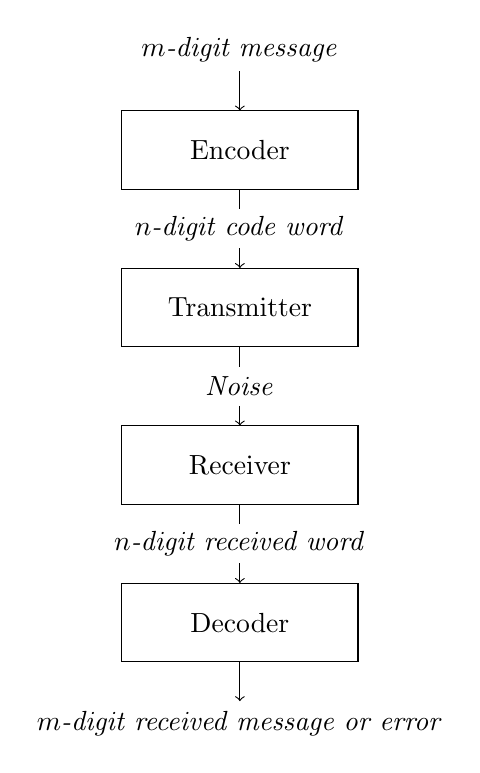
\begin{tikzpicture}[scale=1]

\draw [->] (0,8)  node [above] {\emph{$m$-digit message}} -- (0,7.5);

\node at (0,7) {Encoder};
\draw (-1.5,6.5) rectangle (1.5,7.5);
\draw (0,6.5)  -- (0,6.25);
\draw [->] (0,5.75)  -- (0,5.5);
\node at (0,6) {\emph{$n$-digit code word}};

\node at (0,5) {Transmitter};
\draw (-1.5,4.5) rectangle (1.5,5.5);
\draw (0,4.5)  -- (0,4.25);
\draw [->] (0,3.75)  -- (0,3.5);
\node at (0,4) {\emph{Noise}};

\node at (0,3) {Receiver};
\draw (-1.5,2.5) rectangle (1.5,3.5);
\draw (0,2.5)  -- (0,2.25);
\draw [->] (0,1.75)  -- (0,1.5);
\node at (0,2) {\emph{$n$-digit received word}};

\node at (0,1) {Decoder};
\draw (-1.5,0.5) rectangle (1.5,1.5);
\draw [->] (0,0.5)  -- (0,0) node [below] {\emph{$m$-digit received message or error}};

\end{tikzpicture}

\caption{Encoding and decoding messages}
\end{center}
\label{encoding}
\end{figure}

Uncoded messages may be composed of letters or characters, but
typically they consist of binary $m$-tuples. These messages are
encoded into codewords, consisting of binary $n$-tuples, by a device
called an \boldemph{encoder}. The message is transmitted and then decoded.
We will consider the occurrence of errors during transmission. An
\boldemph{error} occurs if there is a change in one or more bits in the
codeword. A \boldemph{decoding scheme} is a method that either converts
an arbitrarily received $n$-tuple into a meaningful decoded message or
gives an error message for that $n$-tuple. If the received message is
a codeword (one of the special $n$-tuples allowed to be transmitted),
then the decoded message must be the unique message that was encoded
into the codeword. For received non-codewords, the decoding scheme will
give an error indication, or, if we are more clever, will actually try
to correct the error and reconstruct the original message. Our goal is
to transmit error-free messages as cheaply and quickly as possible.
 
 
\begin{example}{repeat}
One possible coding scheme would be to send a message several
times and to compare the received copies with one another. Suppose
that the message to be encoded is a binary $n$-tuple $(x_{1}, x_{2},
\ldots, x_{n})$. The message is encoded into a binary $3n$-tuple by
simply repeating the message three times: 
\[
(x_{1}, x_{2}, \ldots, x_{n})
\mapsto
(x_{1}, x_{2}, \ldots, x_{n}, x_{1}, x_{2}, \ldots, x_{n},
x_{1}, x_{2}, \ldots, x_{n}).
\]
To decode the message, we choose as the $i$th digit the one that
appears in the $i$th place in at least two of the three transmissions.
For example, if the original message is $(0110)$, then the transmitted
message will be \mbox{$(0110\;  0110\;  0110)$}. If there is a transmission error
in the fifth digit, then the received codeword will be
$(0110\;  1110\;  0110)$, which will be correctly decoded as
$(0110)$.\footnote{We will adopt the convention that bits are numbered
left to right in binary $n$-tuples.} 
This triple-repetition method will automatically detect and correct
all single errors, but it is slow and inefficient: to send a message
consisting of $n$ bits, $2n$ extra bits are required, and we can only
detect and correct single errors. We will see that it is possible to
find an encoding scheme that will encode a message of $n$ bits into
$m$ bits with $m$ much smaller than $3n$.
\end{example}
 
 
\begin{example}{even_parity}
\boldemph{Even parity}, a  commonly  used coding scheme, is much
more efficient than the simple repetition scheme. The ASCII (American
Standard Code for Information Interchange) coding system uses binary
8-tuples, yielding $2^{8} = 256$ possible 8-tuples. However, only seven
bits are needed since there are only $2^7 = 128$ ASCII characters.
What can or should be done with the extra bit? Using the full eight
bits, we can detect single transmission errors. For example, the ASCII
codes for A, B, and C are 
\begin{align*}
\mbox{A} & = 65_{10} = 01000001_{2}, \\
\mbox{B} & = 66_{10} = 01000010_{2}, \\
\mbox{C} & = 67_{10} = 01000011_{2}.
\end{align*}
Notice that the leftmost bit is always set to 0; that is, the 128 ASCII
characters have codes 
\begin{align*}
00000000_{2} & = 0_{10}, \\
& \vdots \\
01111111_{2} & = 127_{10}.
\end{align*}
The bit can be used for error checking on the other seven bits. It is
set to either 0 or 1 so that the total number of 1 bits in the
representation of a character is even. Using even parity, the codes
for A, B, and C now become 
\begin{align*}
\mbox{A} & = 01000001_{2}, \\
\mbox{B} & = 01000010_{2}, \\
\mbox{C} & = 11000011_{2}.
\end{align*}
Suppose an A is sent and a transmission error in the sixth
bit is caused by noise over the communication channel so that 
(0100\; 0101) is received. We know an error has occurred since the
received word has an odd number of 1's, and we can now request that the
codeword be transmitted again. When used for error checking, the
leftmost bit is called a \boldemph{parity check bit}.  
 
 
By far the most common error-detecting
codes used in computers are based on the addition of a parity bit.
Typically, a computer stores information in $m$-tuples called \boldemph{
words}. Common word lengths are 8, 16, and 32 bits. One bit in the 
word is set aside as the parity check bit, and is not used to store
information. This bit is set to either 0 or 1, depending on the
number of 1's in the word. 
 
 
Adding a parity check bit allows the detection of all single errors
because changing a single bit either increases or decreases the number
of 1's by one, and in either case the parity has been changed from
even to odd, so the new word is not a codeword. (We could also
construct an error detection scheme based on \boldemph{odd parity}; that
is, we could set the parity check bit so that a codeword always has an
odd number of 1's.)  
\end{example}
 
 
The even parity system is easy to implement, but has two drawbacks.
First, multiple errors are not detectable. Suppose an A is sent and 
the first and seventh bits are changed from 0 to 1. The received word
is a codeword, but will be decoded into a C instead of an A.
Second, we do not have the ability to correct errors.  If the 8-tuple
(1001\; 1000) is received, we know that an error has occurred, but we
have no idea which bit has been changed. We will now investigate a
coding scheme that will not only allow us to detect transmission
errors but will actually correct the errors. 

 
 
\begin{table}[htb]\label{repetition_code}
\begin{center}{\small
\begin{tabular}{|lc|cccccccc|}
\hline
& & \multicolumn{8}{|c|}{Received Word}    \\
            &     & 000 & 001 & 010 & 011 & 100 & 101 & 110
& 111 \\ \hline
Transmitted & 000 & 0   & 1   & 1   & 2   & 1   & 2   & 2
& 3 \\
Codeword   & 111 & 3   &  2  & 2   &  1  &  2  &   1 &  1
&  0 \\ \hline
\end{tabular}
}
\caption{A repetition code}
\end{center}
\end{table}

 
\begin{example}{nearest}
Suppose that our original message is either a 0 or a 1, and that 0
encodes to (000) and 1 encodes to (111). If only a single
error occurs during transmission, we can detect and correct the
error. For example, if a 101 is received, then the second bit must
have been changed from a 1 to a 0.  The originally transmitted
codeword must have been (111). 	This method will detect and correct 
all single errors. 
 
 
In Table~\ref{repetition_code}, we present all possible words that might be received
for the transmitted codewords (000) and (111). Table~\ref{repetition_code} also shows 
the number of bits by which each received 3-tuple differs from each
original codeword. 
\end{example}
 
 
 
\subsection*{Maximum-Likelihood Decoding}

%% Footnote in subsection header undigestable by tex4ht
%%   it can follow just outside the {},
%%   but formats weirdly in both PDF and XHTML
%% \footnote{This section
%% requires a knowledge of probability, but can be
%% skipped without loss of continuity.}

%Label repaired.  Suggested by R. Beezer.
%TWJ - 12/19/2011
The coding scheme presented in Example~\ref{example:algcodes:nearest} is not a complete solution to
the problem because it does not account for the possibility of
multiple errors. For example, either a (000) or a (111) could be sent
and a (001) received. We have no means of deciding from the received
word whether there was a single error in the third bit or two errors,
one in the first bit and one in the second.  No matter what coding 
scheme is used, an incorrect message could
be received: we could transmit a (000), have errors in all three
bits, and receive the codeword (111). It is important to make explicit
assumptions about the likelihood and distribution of transmission
errors so that, in a particular application, it will be known whether
a given
error detection scheme is appropriate. We will assume that
transmission errors are rare, and, that when they do occur, they occur
independently in each bit; that is, if $p$ is the probability of an
error in one bit and $q$ is the probability of an error in a different
bit, then the probability of errors occurring in both of these bits at
the same time is $pq$. We will also assume that a received $n$-tuple 
is
decoded into a codeword that is closest to it; that is, we assume that
the receiver uses \boldemph{maximum-likelihood
decoding}\index{Maximum-likelihood decoding}.
 
 
\begin{figure}[htb]  %Replaced figure with tikz figure - TWJ 5/10/2010
\begin{center}
\tikzpreface{algcode_binary_channel}
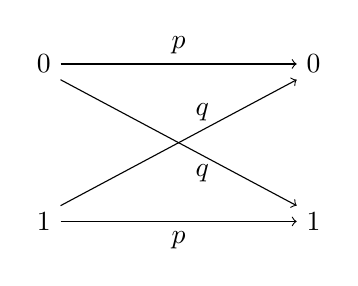
\begin{tikzpicture}[scale=1]

\node at (1.5,0) [below] {$p$};
\draw [->] (0,0)  node [left] {1} -- (3,0) node [right] {1};
\node at (1.5,2) [above] {$p$};
\draw [->] (0,2)  node [left] {0} -- (3,2) node [right] {0};

\draw [->] (0,0.2) -- (3,1.8);
\draw [->] (0,1.8) -- (3,0.2);

\node at (1.8,1.15) [above] {$q$};
\node at (1.8,0.85) [below] {$q$};


\end{tikzpicture}

\end{center}
\caption{Binary symmetric channel}
\label{channel}
\end{figure}
 
 
 
A \boldemph{binary symmetric channel}\index{Binary symmetric channel}
is a model that consists of a transmitter capable of sending a binary 
signal, either a 0 or a 1, together with a receiver. Let $p$ be the 
probability that the signal is correctly
received. Then $q=1-p$ is the probability of an incorrect reception.
If a 1 is sent, then the probability that a 1 is received is $p$ and
the probability that a 0 is received is $q$ (Figure~\ref{channel}).
The probability that no errors occur during the transmission of a binary
codeword of length $n$ is $p^{n}$. For example, if $p=0.999$ and a
message consisting of 10,000 bits is sent, then the probability of a
perfect transmission is 
\[
(0.999)^{10,000} \approx 0.00005.
\]
 
 
\begin{theorem}
If a binary $n$-tuple $(x_{1}, \ldots, x_{n})$ is transmitted across a
binary symmetric channel with probability $p$ that no error will occur
in each coordinate, then the probability that there are errors in
exactly $k$ coordinates~is
\[
\binom{n}{k} q^kp^{n-k}.
\]
\end{theorem}
 
 
\begin{proof}
Fix $k$ different coordinates. We first compute the probability that
an error has occurred in this fixed set of coordinates. The
probability of an error occurring in a particular one of these $k$
coordinates is $q$; the probability that an error will not occur
in any of the remaining $n-k$ coordinates is $p$. The
probability of each of these $n$ independent events is
$q^{k}p^{n-k}$. The number of possible error patterns with exactly $k$
errors occurring is equal to 
\[
\binom{n}{k} 
= \frac{n!}{k!(n-k)!},
\]
the number of combinations of $n$ things taken $k$ at a time. Each of
these error patterns has probability $q^{k}p^{n-k}$ of occurring;
hence, the probability of all of these error patterns is
\[
\binom{n}{k} 
q^{k}p^{n-k}.
\]
\end{proof}
 
 
\begin{example}{probability}
Suppose that $p = 0.995$ and a 500-bit message is sent. The
probability that the message was sent error-free is 
\[
p^{n} = (0.995)^{500} \approx 0.082.
\]
The probability of exactly one error occurring is
\[
\binom{n}{1} 
qp^{n-1}= 500(0.005)(0.995)^{499}
\approx 0.204.
\]
The probability of exactly two errors is
\[
\binom{n}{2} 
q^{2}p^{n-2}=
\frac{500 \cdot 499}{2}(0.005)^{2}(0.995)^{498} \approx
0.257.
\]
The probability of more than two errors is approximately
\[
1-0.082-0.204 -0.257=0.457.
\]
\end{example}
 
 
\subsection*{Block Codes}
 
 
If we are to develop efficient error-detecting and error-correcting
codes, we will need more sophisticated mathematical tools.  Group
theory  will allow faster methods of encoding and decoding messages. A
code is an $(n, m)$-\boldemph{block code} if the information that is to be
coded can be divided into blocks of $m$ binary digits, each of which
can be encoded into $n$ binary digits. More specifically, an $(n,
m)$-block code consists of an \boldemph{encoding function} 
\[
E:{\mathbb Z}^{m}_{2} \rightarrow {\mathbb Z}^{n}_{2}
\]
and a \boldemph{decoding function}
\[
D:{\mathbb Z}^{n}_{2} \rightarrow {\mathbb Z}^{m}_{2}.
\]
A \boldemph{codeword} is any element in the image of $E$. We also require
that $E$ be one-to-one so that two information blocks will not be
encoded into the same codeword. If our code is to be error-correcting,
then $D$ must be onto.
 
 
\begin{example}{BlockCode}
The even-parity coding system developed to detect single errors in
ASCII characters is an $(8,7)$-block code. The encoding function is
\[
E(x_7, x_6, \ldots, x_1) = (x_8, x_7,  \ldots, x_1),
\]
where $x_8 = x_7 + x_6 + \cdots + x_1$ with addition in ${\mathbb Z}_2$. 
\end{example}
 

 
Let ${\mathbf x} = (x_1, \ldots, x_n)$ and ${\mathbf y} = (y_1, \ldots,
y_n)$ be binary $n$-tuples. The \boldemph{Hamming distance}\index{Hamming
distance} or \boldemph{distance}, $d({\mathbf x}, {\mathbf
y})$\label{noteHammingdist}, between ${\mathbf x}$ and ${\mathbf y}$ is
the number of bits in which ${\mathbf x}$ and ${\mathbf y}$ differ. The
distance between two codewords is the minimum number of transmission
errors required to change one codeword into the other. The
\boldemph{minimum distance}\index{Code!minimum distance of} for a code,
$d_{\min}$\label{notemindist}, is the minimum of all distances
$d({\mathbf x}, {\mathbf y})$, where ${\mathbf x}$ and ${\mathbf y}$ are
distinct codewords. The \boldemph{weight}\index{Weight of a codeword},
$w({\mathbf x})$\label{noteweight}, of a binary codeword ${\mathbf x}$ is
the number of 1's in ${\mathbf x}$. Clearly, $w({\mathbf x}) = d({\mathbf
x}, {\mathbf 0})$, where ${\mathbf 0} = (00 \cdots 0)$. 
 
 
\begin{example}{min_distance}
Let ${\mathbf x} = (10101)$, ${\mathbf y} = (11010)$, and ${\mathbf z} =
(00011)$ be all of the codewords in some code $C$. Then we have the
following Hamming distances: 
\[
d({\mathbf x},{\mathbf y}) = 4, \qquad
d({\mathbf x},{\mathbf z}) = 3, \qquad
d({\mathbf y},{\mathbf z}) = 3.
\]
The minimum distance  for this code is 3. We also have the
following weights: 
\[
w({\mathbf x}) = 3, \qquad
w({\mathbf y}) = 3, \qquad
w({\mathbf z}) = 2.
\]
\end{example}
 
 
The following proposition lists some basic properties about the weight
of a codeword and the distance between two codewords. The proof is
left as an exercise.
 
 
\begin{proposition}
Let ${\mathbf x}$, ${\mathbf y}$, and ${\mathbf z}$ be binary $n$-tuples.
Then 
\begin{enumerate}
 
\rm \item \it
$w({\mathbf x}) = d( {\mathbf x}, {\mathbf 0})$; 
 
\rm \item \it
$d( {\mathbf x}, {\mathbf y}) \geq 0$; 
 
\rm \item \it
$d( {\mathbf x}, {\mathbf y}) = 0$ exactly when ${\mathbf x} = {\mathbf y}$; 
 
\rm \item \it
$d( {\mathbf x}, {\mathbf y})= d( {\mathbf y}, {\mathbf x})$; 
 
\rm \item \it
$d( {\mathbf x}, {\mathbf y}) \leq d( {\mathbf x}, {\mathbf z}) + d( {\mathbf
z}, {\mathbf y})$. 
 
\end{enumerate}
\end{proposition}
 
 
The weights in a particular code are usually much easier to compute
than the Hamming distances between all codewords in the code. If a
code is set up carefully, we can use this fact to our advantage.
 
 
Suppose that ${\mathbf x} = (1101)$ and ${\mathbf y} = (1100)$ are
codewords in some code. If we transmit (1101) and an error occurs in
the rightmost bit, then (1100) will be received. Since (1100) is a
codeword, the decoder will decode (1100) as the transmitted message.
This code is clearly not very appropriate for error detection. The
problem is that $d({\mathbf x}, {\mathbf y}) = 1$. If ${\mathbf x} = (1100)$
and ${\mathbf y} = (1010)$ are codewords, then $d({\mathbf x}, {\mathbf y})
= 2$. If ${\mathbf x}$ is transmitted and a single error occurs, then
${\mathbf y}$ can never be received. Table~\ref{4-bit_words} gives the distances
between all 4-bit codewords in which the first three bits carry
information and the fourth is an even parity check bit. We can see
that the minimum distance here is 2; hence, the code is suitable as
a single error-correcting code. 
 
 
\begin{table}[hbt]
{\small
\begin{center}
\begin{tabular}{|c|cccccccc|}
\hline
    & 0000 & 0011 & 0101 & 0110 & 1001 & 1010 & 1100 & 1111
\\ \hline
0000 & 0 & 2 & 2 & 2 & 2 & 2 & 2 & 4 \\
0011 & 2 & 0 & 2 & 2 & 2 & 2 & 4 & 2 \\
0101 & 2 & 2 & 0 & 2 & 2 & 4 & 2 & 2 \\
0110 & 2 & 2 & 2 & 0 & 4 & 2 & 2 & 2 \\
1001 & 2 & 2 & 2 & 4 & 0 & 2 & 2 & 2 \\
1010 & 2 & 2 & 4 & 2 & 2 & 0 & 2 & 2 \\
1100 & 2 & 4 & 2 & 2 & 2 & 2 & 0 & 2 \\
1111 & 4 & 2 & 2 & 2 & 2 & 2 & 2 & 0 \\
\hline
\end{tabular}
\caption{Distances between 4-bit codewords}\label{4-bit_words}
\end{center}
}
\end{table}
 
 
 
To determine exactly what the error-detecting and error-correcting
capabilities for a code are, we need to analyze the minimum distance
for the code. Let ${\mathbf x}$ and ${\mathbf y}$ be codewords. If
$d({\mathbf x}, {\mathbf y}) = 1$ and an error occurs where ${\mathbf x}$
and ${\mathbf y}$ differ, then ${\mathbf x}$ is changed to ${\mathbf y}$.
The received codeword is ${\mathbf y}$ and no error message is given.
Now suppose $d({\mathbf x}, {\mathbf y}) = 2$. Then a single error cannot
change ${\mathbf x}$ to ${\mathbf y}$. Therefore, if $d_{\min} = 2$, we
have the ability to detect single errors. However, suppose that
$d({\mathbf x}, {\mathbf y}) = 2$, ${\mathbf y}$ is sent, and a noncodeword
${\mathbf z}$ is received such that
\[
d({\mathbf x}, {\mathbf z}) = d({\mathbf y}, {\mathbf z}) = 1.
\]
Then the decoder cannot decide between ${\mathbf x}$ and ${\mathbf y}$. Even
though we are aware that an error has occurred, we do not know what
the error is.
 
 
Suppose $d_{\min} \geq 3$. Then the maximum-likelihood decoding scheme
corrects all single errors. Starting with a codeword ${\mathbf x}$, an
error in the transmission of a single bit gives ${\mathbf y}$ with
$d({\mathbf x}, {\mathbf y}) = 1$, but $d({\mathbf z}, {\mathbf y}) \geq 2$
for any other codeword ${\mathbf z} \neq {\mathbf x}$. If we do not
require the correction of errors, then we can detect multiple errors
when a code has a minimum distance that is greater than 3.  
 
 
\begin{theorem}\label{algecodes:min_distance_theorem}
Let $C$ be a code with $d_{\min} = 2n + 1$. Then $C$ can correct any
$n$ or fewer errors.  Furthermore, any $2n$ or fewer errors can be
detected in~$C$. 
\end{theorem}
 
 
\begin{proof}
Suppose that a codeword ${\mathbf x}$ is sent and the word ${\mathbf y}$
is received with at most $n$ errors. Then $d( {\mathbf x}, {\mathbf y})
\leq n$. If ${\mathbf z}$ is any codeword other than ${\mathbf x}$, then
\[
2n+1
\leq
d( {\mathbf x}, {\mathbf z})
\leq
d( {\mathbf x}, {\mathbf y}) + d( {\mathbf y}, {\mathbf z})
\leq
n + d( {\mathbf y}, {\mathbf z}).
\]
Hence, $d({\mathbf y}, {\mathbf z} ) \geq n+1$ and ${\mathbf y}$ will be
correctly decoded as ${\mathbf x}$. Now suppose that ${\mathbf x}$ is
transmitted and ${\mathbf y}$ is received and that at least one error 
has occurred, but not more than $2n$ errors. Then $1 \leq d( {\mathbf x},
{\mathbf y} ) \leq 2n$.  Since the minimum distance between codewords is
$2n +1$, ${\mathbf y}$ cannot be a codeword.  Consequently, the code can
detect between 1 and $2n$ errors. 
\end{proof}
 
 
\begin{example}{single_correct}
In Table~\ref{Hamming_dist}, the codewords ${\mathbf c}_1 = (00000)$, ${\mathbf c}_2 = (00111)$,
${\mathbf c}_3 = (11100)$, and ${\mathbf c}_4 = (11011)$ determine a
single error-correcting code.  
\end{example}
 
 
\begin{table}[htb]

\begin{center}
{\small
\begin{tabular}{|c|cccc|}
\hline
      & 00000 & 00111 & 11100 & 11011 \\ \hline
00000 & 0     & 3     & 3     & 4 \\
00111 & 3     & 0     & 4     & 3 \\
11100 & 3     & 4     & 0     & 3 \\
11011 & 4     & 3     & 3     & 0 \\
\hline
\end{tabular}
}
\caption{ Hamming distances for an error-correcting code}\label{Hamming_dist}
\end{center}
\end{table}
 
 
 
 
 
\histhead
 
 
\noindent{\small \histf
Modern coding theory began in 1948 with C. Shannon's\index{Shannon,
C.} paper, ``A Mathematical Theory of Information'' [7]. This paper offered
an example of an algebraic code, and Shannon's Theorem proclaimed
exactly how good codes could be expected to be. Richard
Hamming\index{Hamming, R.} began working with linear codes at Bell
Labs in the late 1940s and early 1950s after becoming frustrated
because the programs that he was running could not recover from simple
errors generated by noise. Coding theory has grown tremendously in the
past several years. \textit{The Theory of Error-Correcting Codes}, by 
MacWilliams and Sloane [5], published in 1977, already
contained over 1500 references. Linear codes (Reed-Muller $(32,
6)$-block codes) were used on NASA's Mariner space probes.  More recent
space probes such as Voyager have used what are called convolution
codes.  Currently, very active research is being done with Goppa
codes, which are heavily dependent on algebraic geometry.
\histbox
} 
 
 
\section{Linear Codes}
 
 
To gain more knowledge of a particular code and develop more efficient
techniques of encoding, decoding, and error detection, we need to add
additional structure to our codes. One way to accomplish this is to
require that the code also be a group. A \boldemph{group
code}\index{Code!group} is a code that is also a subgroup of ${\mathbb
Z}_2^n$.  
 
 
To check that a code is a group code, we need only verify one thing.
If we add any two elements in the code, the result must be an $n$-tuple
that is again in the code. It is not necessary to check that the
inverse of the $n$-tuple is in the code, since every codeword is its own
inverse, nor is it necessary to check that ${\mathbf 0}$ is a codeword.
For instance,
\[
(11000101) + (11000101) = (00000000).
\]
 
 
\begin{example}{weights}
Suppose that we have a code that consists of the following 7-tuples: 
\[
\begin{array}{cccc}
(0000000) & (0001111) & (0010101) & (0011010) \\
(0100110) & (0101001) & (0110011) & (0111100) \\
(1000011) & (1001100) & (1010110) & (1011001) \\
(1100101) & (1101010) & (1110000) & (1111111).
\end{array}
\]
It is a straightforward though tedious task to verify that this code
is also a subgroup of ${\mathbb Z}_2^7$ and, therefore, a group code.
This code is a single error-detecting and single error-correcting 
code, but
it is a long and tedious process to compute all of the distances
between  pairs of codewords to determine that $d_{\min} = 3$. It is
much easier to see that the minimum weight of all the nonzero
codewords is 3. As we will soon see, this is no coincidence.
However, the relationship between weights and distances in a
particular code is heavily dependent on the fact that the code is a
group. 
\end{example}
 
 
\begin{lemma}
Let ${\mathbf x}$ and ${\mathbf y}$ be  binary $n$-tuples. Then $w({\mathbf
x} + {\mathbf y}) = d({\mathbf x}, {\mathbf y})$. 
\end{lemma}
 
 
\begin{proof}
Suppose that ${\mathbf x}$ and ${\mathbf y}$ are binary $n$-tuples. Then
the distance between ${\mathbf x}$ and ${\mathbf y}$ is exactly the number
of places in which ${\mathbf x}$ and ${\mathbf y}$ differ. But ${\mathbf x}$
and ${\mathbf y}$ differ in a particular coordinate exactly when the sum
in the coordinate is 1, since
\begin{align*}
1 + 1 & = 0 \\
0 + 0 & = 0 \\
1 + 0 & = 1 \\
0 + 1 & = 1.
\end{align*}
Consequently, the weight of the sum must be the distance between the two
codewords.
\end{proof}
 
 
\begin{theorem}
Let $d_{\min}$ be the minimum distance for a group code $C$. Then
$d_{\min}$ is the minimum of all the nonzero weights of the nonzero
codewords in $C$. That is, 
\[
d_{\min} = \min\{ w({\mathbf x}) : { {\mathbf x} \neq {\mathbf 0} } \}.
\]
\end{theorem}
 
 
\begin{proof}
Observe that
\begin{align*}
d_{\min} & =  \min \{ d({\mathbf x},{\mathbf y}) : {\mathbf x}
\neq
{\mathbf y} \} \\
&=  \min \{ d({\mathbf x},{\mathbf y}) : {\mathbf x}+{\mathbf y}
\neq {\mathbf 0} \} \\
&= \min\{ w({\mathbf x} + {\mathbf y}) : {\mathbf x}+{\mathbf y}
\neq {\mathbf 0} \} \\
& =  \min\{ w({\mathbf z}) : {\mathbf z} \neq {\mathbf 0} \}.
\end{align*}
\end{proof}
 
 
\subsection*{Linear Codes}
 
 
From Example~\ref{example:algcodes:weights}, it is now easy to check that the minimum nonzero
weight is 3; hence, the code does indeed detect and correct all
single errors. We have now reduced the problem of finding ``good''
codes to that of generating group codes. One easy way to generate
group codes is to employ a bit of matrix theory. 
 
 
Define the \boldemph{inner product}\index{Inner product} of two binary
$n$-tuples to be 
\[
{\mathbf x} \cdot {\mathbf y} = x_1 y_1 + \cdots + x_n y_n,
\]
where ${\mathbf x} = (x_1, x_2, \ldots, x_n)^{\rm t}$ and ${\mathbf y} =
(y_1, y_2, \ldots, y_n)^{\rm t}$ are column vectors.\footnote{Since we
will be working with matrices, we will write binary $n$-tuples as
column vectors for the remainder of this chapter.} For example, if
${\mathbf x} = (011001)^{\rm t}$ and ${\mathbf y} = (110101)^{\rm t}$,
then ${\mathbf x} \cdot {\mathbf y} = 0$. We can also look at an inner
product as the product of a row matrix with a column matrix; that is, 
\begin{align*}
{\mathbf x} \cdot {\mathbf y} & = {\mathbf x}^{\rm t}  {\mathbf y}
\\
& =
\begin{pmatrix}
x_1 & x_2 & \cdots & x_n
\end{pmatrix}
\begin{pmatrix}
y_1 \\
y_2 \\
\vdots \\
y_n
\end{pmatrix} \\
& =
x_{1}y_{1} + x_{2}y_{2} + \cdots + x_{n}y_{n}.
\end{align*}
 
 
\begin{example}{matrix_codes}
Suppose that the words to be encoded consist of all binary
\mbox{3-tuples}
and that our encoding scheme is even-parity. To encode an arbitrary
3-tuple, we add a fourth bit to obtain an even number of 1's. Notice
that an arbitrary $n$-tuple ${\mathbf x} = (x_1, x_2, \ldots, x_n)^{\rm
t}$ has an even number of 1's exactly when $x_1 + x_2 + \cdots + x_n =
0$; hence, a 4-tuple ${\mathbf x} = (x_1, x_2, x_3, x_4)^{\rm t}$ has an
even number of 1's if $ x_1+ x_2+ x_3+ x_4 = 0$, or 
\[
{\mathbf x} \cdot {\mathbf 1} 
= 
{\mathbf x}^{\rm t} {\mathbf 1} 
=
\begin{pmatrix}
x_1 & x_2 & x_3 & x_4
\end{pmatrix}
\begin{pmatrix}
1 \\ 1 \\ 1 \\ 1
\end{pmatrix} = 0.
\]
This example leads us to hope that there is a connection between
matrices and coding theory. 
\end{example}
 
 
Let ${\mathbb M}_{m \times n}({\mathbb Z}_2)$\label{notembyn} denote the set
of all $m \times n$ matrices with entries in ${\mathbb Z}_2$. We do
matrix operations as usual except that all our addition and multiplication
operations occur in ${\mathbb Z}_2$. Define the \boldemph{null
space}\index{Matrix!null space of}\index{Null space!of a matrix} of 
a matrix $H \in {\mathbb M}_{m \times n}({\mathbb Z}_2)$ to be the set of
all binary $n$-tuples ${\mathbf x}$ such that $H{\mathbf x} = {\mathbf 0}$.
We denote the null space of a matrix $H$ by ${\rm Null}(H)$\label{notenull}.  
 
 
\begin{example}{group_code}
Suppose that
\[
H =
\begin{pmatrix}
0 & 1 & 0 & 1 & 0 \\
1 & 1 & 1 & 1 & 0 \\
0 & 0 & 1 & 1 & 1
\end{pmatrix}.
\]
For a 5-tuple ${\mathbf x} = (x_1, x_2, x_3, x_4, x_5)^{\rm t}$ to be in
the null space of $H$, $H{\mathbf x} = {\mathbf 0}$. Equivalently, the
following system of equations must be satisfied:   
\begin{align*}
  x_2 +  x_4  & =  0 \\
x_1 +  x_2 + x_3  + x_4   & =  0 \\
  x_3  + x_4  +  x_5 & =  0.
\end{align*}
The set of binary 5-tuples satisfying these equations is
\[
(00000) \qquad (11110) \qquad (10101) \qquad (01011).
\]
This code is easily determined to be a group code.
\end{example}
 
 
\begin{theorem}
Let $H$ be in ${\mathbb M}_{m \times n}({\mathbb Z}_2)$. Then the null space of
$H$ is a group~code. 
\end{theorem}
 
 
\begin{proof}
Since each element of ${\mathbb Z}_2^n$ is its own inverse, the only
thing that really needs to be checked here is closure. Let ${\mathbf x},
{\mathbf y} \in {\rm Null}(H)$ for some matrix $H$ in ${\mathbb M}_{m \times
n}({\mathbb Z}_2)$. Then $H{\mathbf x} = {\mathbf 0}$ and $H{\mathbf y} =
{\mathbf 0}$. So 
\[
H({\mathbf x}+{\mathbf y}) 
=
H{\mathbf x} + H{\mathbf y} = {\mathbf 0}
+
{\mathbf 0}
= {\mathbf 0}.
\]
Hence, ${\mathbf x}+{\mathbf y}$ is in the null space of $H$ and
therefore must be a codeword. 
\hspace*{1in}
\end{proof}
 
%typo correction.  Suggested by J. Buller.
%TWJ - 12/20/2011

\medskip
 
 
A code is a \boldemph{linear code}\index{Code!linear} if it is
determined by the null space of some matrix $H \in {\mathbb M}_{m \times
n}({\mathbb Z}_2)$.  
 
 
 
\begin{example}{linear_code}
Let $C$ be the code given by the matrix
\[
H =
\begin{pmatrix}
0 & 0 & 0 & 1 & 1 & 1 \\
0 & 1 & 1 & 0 & 1 & 1 \\
1 & 0 & 1 & 0 & 0 & 1
\end{pmatrix}.
\]
Suppose that the 6-tuple ${\mathbf x} = (010011)^{\rm t}$ is received.
It is a simple matter of matrix multiplication to determine whether or
not ${\mathbf x}$ is a codeword. Since 
\[
H{\mathbf x} =
\begin{pmatrix} 
0 \\ 1 \\ 1
\end{pmatrix},
\]
the received word is not a codeword.  We must either attempt to
correct the word or request that it be transmitted again.
\end{example}

%typo correction.  Suggested by J. Buller.
%TWJ - 12/20/2011
 
 
 
\section{Parity-Check and Generator Matrices}
 
 
We need to find a systematic way of generating linear codes as well as
fast methods of decoding. By examining the properties of a matrix $H$
and by carefully choosing $H$, it is possible to develop very
efficient methods of encoding and decoding messages. To this end, we 
will introduce standard generator and canonical parity-check
matrices.
 
 
Suppose that $H$ is an $m \times n$ matrix with entries in
${\mathbb Z}_2$ and $n > m$. If the last $m$ columns of the
matrix form the $m \times m$ identity matrix, $I_m$, then
the matrix is a \boldemph{canonical parity-check
matrix}\index{Matrix!parity-check}. More specifically, $H= (A \mid I_m
)$, where $A$ is the $m \times (n-m)$ matrix
\[
\begin{pmatrix}
a_{11} & a_{12} & \cdots & a_{1,n-m} \\
a_{21} & a_{22} & \cdots & a_{2,n-m} \\
\vdots & \vdots \ddots & \vdots    \\
a_{m1} & a_{m2} & \cdots & a_{m,n-m}
\end{pmatrix}
\]
and $I_m$ is the $m \times m$ identity matrix
\[
\begin{pmatrix}
1 & 0 & \cdots & 0 \\
0 & 1 & \cdots & 0 \\
\vdots & \vdots \ddots & \vdots \\
0 & 0 & \cdots & 1
\end{pmatrix}.
\]
With each canonical parity-check matrix we can associate an $n \times
(n-m)$ \boldemph{standard generator matrix}\index{Matrix!generator} 
\[
G =
\left(
\frac{I_{n-m}}{A}
\right).
\]
Our goal will be to show that $G {\mathbf x} = {\mathbf y}$ if and only if
$H{\mathbf y} = {\mathbf 0}$.  Given a message block ${\mathbf x}$ to be
encoded, $G$ will allow us to quickly encode it into a linear
codeword ${\mathbf y}$. 
 
 
\begin{example}{ParityCheck}
Suppose that we have the following eight words to be
encoded:
\[
(000), (001), (010), \ldots, (111).
\]
For
\[
A =
\begin{pmatrix}
0 & 1 & 1 \\
1 & 1 & 0 \\
1 & 0 & 1
\end{pmatrix},
\]
the associated standard generator and canonical parity-check matrices
are 
\[
G=
\begin{pmatrix}
1 & 0 & 0 \\
0 & 1 & 0 \\
0 & 0 & 1 \\
0 & 1 & 1 \\
1 & 1 & 0 \\
1 & 0 & 1
\end{pmatrix}
\]
and
\[
H =
\begin{pmatrix}
0 & 1 & 1 & 1 & 0 & 0 \\
1 & 1 & 0 & 0 & 1 & 0 \\
1 & 0 & 1 & 0 & 0 & 1
\end{pmatrix},
\]
respectively.
 
 
Observe that the rows in $H$  represent the parity checks on certain
bit positions in a 6-tuple. The 1's in the identity matrix serve as
parity checks for the 1's in the same row. If ${\mathbf x} = (x_1, x_2,
x_3, x_4, x_5, x_6)$, then 
\[
{\mathbf 0}
=
H{\mathbf x}
=
\begin{pmatrix}
x_2 + x_3 + x_4 \\
x_1 + x_2 + x_5\\
x_1 + x_3 + x_6
\end{pmatrix},
\]
which yields a system of equations:
\begin{align*}
x_2 + x_3 + x_4 & = 0 \\
x_1 + x_2 + x_5 & = 0 \\
x_1 + x_3 + x_6 & = 0.
\end{align*}
Here $x_4$ serves as a check bit for $x_2$ and $x_3$; $x_5$ is a check
bit for $x_1$ and $x_2$; and $x_6$ is a check bit for $x_1$ and $x_3$.
The identity matrix keeps $x_4$, $x_5$, and $x_6$ from having to check
on each other. Hence, $x_1$, $x_2$, and $x_3$ can be arbitrary but
$x_4$, $x_5$, and $x_6$ must be chosen to ensure parity. The null
space of $H$ is easily computed to be
\[
\begin{array}{cccc}
 (000000) & (001101) & (010110) & (011011) \\
 (100011) & (101110) & (110101) & (111000).
\end{array}
\]
An even easier way to compute the null space is with the generator
matrix $G$ (Table~\ref{matrix_gen_code}). 
\end{example}
 
 
\begin{table}[htb]
{\small
\begin{center}
\begin{tabular}{|c|c|}
\hline
Message Word  & Codeword \\
${\mathbf x}$ & $G {\mathbf x}$ \\ \hline
000 & 000000 \\
001 & 001101 \\
010 & 010110 \\
011 & 011011 \\
100 & 100011 \\
101 & 101110 \\
110 & 110101 \\
111 & 111000 \\
\hline
\end{tabular}
\end{center}
}
\caption{A matrix-generated code}\label{matrix_gen_code}
\end{table}
 
 
\begin{theorem}
If $H \in {\mathbb M}_{m \times n}({\mathbb Z}_2)$ is a canonical
parity-check matrix, then ${\rm Null}(H)$ consists of all 
${\mathbf x} \in {\mathbb Z}_2^n$ whose first $n-m$ bits are arbitrary but whose last $m$ bits
are determined by $H{\mathbf x} = {\mathbf 0}$. Each of
the last $m$ bits serves as an even parity check bit for some of the
first $n-m$ bits. Hence, $H$ gives rise to an $(n, n-m)$-block code. 
\end{theorem}


 
 
We leave the proof of this theorem as an exercise. In light of the
theorem, the first $n - m$ bits in ${\mathbf x}$ are called \boldemph{
information bits} and the last $m$ bits are called \boldemph{check bits}.
In Example~\ref{example:algcodes:ParityCheck},  the first three bits are the information bits
and the last three are the check bits.
 
 
\begin{theorem}
Suppose that $G$ is an $n \times k$  standard generator matrix.  Then
$C = \left\{{\mathbf y} : G{\mathbf x} ={\mathbf y}\text{ for }{\mathbf x}\in
{\mathbb  Z}_2^k\right\}$ is an  $(n,k)$-block code. More specifically, $C$
is a group code.  
\end{theorem}
 
 
\begin{proof}
Let $G {\mathbf x}_1 = {\mathbf y}_1$ and $G {\mathbf
x}_2 ={\mathbf y}_2$ be two codewords. Then ${\mathbf y}_1
+ {\mathbf y}_2$ is in $C$ since 
\[
G( {\mathbf x}_1 + {\mathbf x}_2)
=
G {\mathbf x}_1 + G {\mathbf x}_2
=
{\mathbf y}_1 + {\mathbf y}_2.
\]
We must also show that two message blocks cannot be encoded into the
same codeword. That is, we must show that if $G {\mathbf x} = G
{\mathbf y}$, then ${\mathbf x} = {\mathbf y}$.  Suppose that $G
{\mathbf x} = G {\mathbf y}$. Then
\[
G {\mathbf x} - G {\mathbf y}
=
G( {\mathbf x} - {\mathbf y})
=
{\mathbf 0}.
\]
However, the first $k$ coordinates in $G( {\mathbf x} - {\mathbf
y})$ are exactly $x_1 -y_1, \ldots, x_k - y_k$, since they are
determined by the identity matrix, $I_k$, part of $G$. Hence, $G(
{\mathbf x} - {\mathbf y}) = {\mathbf 0}$ exactly when
${\mathbf x} = {\mathbf y}$.
\end{proof}
 
 \medskip
 
 
Before we can prove the relationship between canonical parity-check
matrices and standard generating matrices, we need to prove a lemma.
 
 
\begin{lemma}\label{ParityCheckLemma}
Let $H = (A \mid I_m )$ be an $m \times n$ canonical parity-check
matrix and $G = \left( \frac{I_{n-m} }{A} \right)$ be the
corresponding $n \times (n-m)$ standard generator matrix. Then $HG =
{\mathbf 0}$. 
\end{lemma}
 
 
\begin{proof}
Let $C = HG$.  The $ij$th entry in $C$ is
\begin{align*}
c_{ij}
& = 
\sum_{k=1}^n h_{ik} g_{kj} \\
& =  \sum_{k=1}^{n-m} h_{ik} g_{kj} + \sum_{k=n-m+1}^n h_{ik} g_{kj} \\
& = \sum_{k=1}^{n-m} a_{ik} \delta_{kj} + \sum_{k=n-m+1}^n \delta_{i-(m-n),k} a_{kj} \\
& =  a_{ij} + a_{ij} \\
& = 0,
\end{align*}
where
\[
\delta_{ij}\label{notekron}
=
\begin{cases}
1, & i = j \\
0, & i \neq j
\end{cases}
\]
is the Kronecker delta\index{Kronecker delta}.
\end{proof}
 
 
\begin{theorem}
Let $H = (A \mid I_m )$ be an $m \times n$ canonical parity-check
matrix and let $G = \left( \frac{I_{n-m} }{A} \right) $ be the $n
\times (n-m)$ standard generator matrix associated with $H$. Let $C$
be the code generated by $G$. Then ${\mathbf y}$ is in $C$ if and only
if $H {\mathbf y} = {\mathbf 0}$. In particular, $C$ is a linear code with
canonical parity-check matrix $H$. 
\end{theorem}
 
 
\begin{proof}
First suppose that ${\mathbf y} \in C$. Then $G {\mathbf x} = {\mathbf y}$
for some ${\mathbf x} \in {\mathbb Z}_2^m$. By Lemma~\ref{ParityCheckLemma}, $H {\mathbf y} = HG
{\mathbf x} = {\mathbf 0}$. 
 
 
Conversely, suppose that ${\mathbf y} = (y_1, \ldots, y_n)^{\rm t}$ is
in the null space of $H$.  We need to find an ${\mathbf x}$ in ${\mathbb
Z}_2^{n-m}$ such that $G {\mathbf x}^{\rm t} = {\mathbf y}$. Since $H
{\mathbf y} = {\mathbf 0}$, the following set of equations must be
satisfied:  
\begin{align*}
a_{11} y_1 + a_{12} y_2 + \cdots + a_{1, n-m} y_{n-m} + y_{n-m+1}
& = 0 \\
a_{21} y_1 + a_{22} y_2 + \cdots + a_{2, n-m} y_{n-m} + y_{n-m+1}
& = 0 \\
& \vdots   \\
a_{m1} y_1 + a_{m2} y_2 + \cdots + a_{m, n-m} y_{n-m} + y_{n-m+1}
& = 0.
\end{align*}
Equivalently, $y_{n-m+1}, \ldots, y_n$ are determined by $y_1, \ldots,
y_{n-m}$: 
\begin{align*}
y_{n-m+1}
& = a_{11} y_1 + a_{12} y_2 + \cdots + a_{1, n-m} y_{n-m} \\
y_{n-m+1}
& = a_{21} y_1 + a_{22} y_2 + \cdots + a_{2, n-m} y_{n-m} \\
& \vdots \\
y_{n-m+1}
& = a_{m1} y_1 + a_{m2} y_2 + \cdots + a_{m, n-m} y_{n-m}.
\end{align*}
Consequently, we can let $x_i = y_i$ for $i= 1, \ldots, n - m$.
\end{proof}
 
 
\medskip
 
 
It would be helpful if we could compute the minimum distance of a
linear code directly from its matrix $H$ in order to determine the
error-detecting and error-correcting capabilities of the code. Suppose
that  
\begin{align*}
{\mathbf e}_1 & = (100 \cdots 00)^{\rm t} \\
{\mathbf e}_2 & = (010 \cdots 00)^{\rm t} \\
 & \vdots \\
{\mathbf e}_n & = (000 \cdots 01)^{\rm t}
\end{align*}
are the $n$-tuples in ${\mathbb Z}_2^n$ of weight 1. For an $m \times
n$ binary matrix $H$, $H{\mathbf e}_i$ is exactly the $i$th column of
the matrix $H$. 
 
 
\begin{example}{ith_column}
Observe that
\[
\begin{pmatrix}
1 & 1 & 1 & 0 & 0 \\
1 & 0 & 0 & 1 & 0 \\
1 & 1 & 0 & 0 & 1
\end{pmatrix}
\begin{pmatrix}
 0 \\ 1 \\ 0 \\ 0 \\ 0
\end{pmatrix}
=
\begin{pmatrix}
1 \\ 0 \\ 1
\end{pmatrix}.
\]
\end{example}
 
 
We state this result in the following proposition and leave the proof
as an exercise. 
 
\begin{proposition}\label{ColumnProp}
Let ${\mathbf e}_i$ be the binary $n$-tuple with a $1$ in the $i$th
coordinate and $0$'s elsewhere and suppose that $H \in {\mathbb M}_{m
\times n}({\mathbb Z}_2)$. Then $H{\mathbf e}_i$ is the $i$th column of
the matrix $H$.  
\end{proposition}
 
 
\begin{theorem}\label{SingleErrorTheorem}
Let $H$ be an $m \times n$ binary matrix. Then the null space of $H$
is a single error-detecting code if and only if no column of $H$
consists entirely of zeros. 
\end{theorem}
 
 
\begin{proof}
Suppose that ${\rm Null}(H)$ is a single error-detecting code. Then the minimum
distance of the code must be at least 2. Since the null space is a
group code, it is sufficient to require that the code contain no
codewords of less than weight 2 other than the zero codeword. That
is, ${\mathbf e}_i$ must not be a codeword for $i = 1, \ldots, n$. Since
$H{\mathbf e}_i$ is the $i$th column of $H$, the only way in which
${\mathbf e}_i$ could be in the null space of $H$ would be if the $i$th
column were all zeros, which is impossible; hence, the code must have
the capability to detect at least single errors.
 
 
Conversely, suppose that no column of $H$ is the zero column. By 
Proposition~\ref{ColumnProp}, $H{\mathbf e}_i \neq {\mathbf 0}$.
\end{proof}
 
 
\begin{example}{null_space}
If we consider the matrices
\[
H_1 =
\begin{pmatrix}
1 & 1 & 1 & 0 & 0 \\
1 & 0 & 0 & 1 & 0 \\
1 & 1 & 0 & 0 & 1
\end{pmatrix}
\]
and
\[
H_2 =
\begin{pmatrix}
1 & 1 & 1 & 0 & 0 \\
1 & 0 & 0 & 0 & 0 \\
1 & 1 & 0 & 0 & 1
\end{pmatrix},
\]
then the null space of $H_1$ is a single error-detecting code and the
null space of $H_2$ is not. 
\end{example}
 
 
We can even do better than Theorem~\ref{SingleErrorTheorem}. This theorem gives us
conditions on a matrix $H$ that tell us when the minimum weight of
the code formed by the null space of $H$ is 2.  We can also
determine when the minimum distance of a linear code is 3 by
examining the corresponding matrix.
 
 
\begin{example}{check_matrix}
If we let
\[
H =
\begin{pmatrix}
1 & 1 & 1 & 0 \\
1 & 0 & 0 & 1 \\
1 & 1 & 0 & 0
\end{pmatrix}
\]
and  want to determine whether or not $H$ is the canonical
parity-check matrix for an error-correcting code, it is necessary to
make certain that ${\rm Null}(H)$ does not contain any 4-tuples of weight
2. That is, $(1100)$, $(1010)$, $(1001)$, $(0110)$, $(0101)$, and
$(0011)$ must not be in ${\rm Null}(H)$.  The next theorem states that 
we can
indeed determine that the code generated by $H$ is error-correcting by
examining the columns of $H$. Notice in this example that not only
does $H$ have no zero columns, but also that no two columns are the
same. 
\end{example}
 
 
\begin{theorem}
Let $H$ be a binary matrix. The null space of $H$ is a single
error-correcting code if and only if $H$ does not contain any zero
columns and no two columns of $H$ are identical.
\end{theorem}
 
 
\begin{proof}
The $n$-tuple ${\mathbf e}_{i} +{\mathbf e}_{j}$ has 1's in the $i$th and
$j$th entries and 0's elsewhere, and $w( {\mathbf e}_{i} +{\mathbf
e}_{j}) = 2$ for $i \neq j$. Since
\[
{\mathbf 0}
= H({\mathbf e}_{i} +{\mathbf e}_{j})
= H{\mathbf e}_{i} + H{\mathbf e}_{j}
\]
can only occur if the $i$th and $j$th columns are identical, the
null space of $H$ is a single error-correcting code.
\end{proof}
 
 
\medskip
 
 
Suppose now that we have a canonical parity-check matrix $H$ with
three rows. Then we might ask how many more columns we can add to
the matrix and still have a null space that is a single
error-detecting and single error-correcting code. Since each column
has three entries, there are $2^3 = 8$ possible distinct columns. We
cannot add the columns 
\[
\begin{pmatrix}
 0 \\ 0 \\ 0 
\end{pmatrix},
\begin{pmatrix}
 1 \\ 0 \\ 0 
\end{pmatrix},
\begin{pmatrix}
 0 \\ 1 \\ 0 
 \end{pmatrix},
\begin{pmatrix}
 0 \\ 0 \\ 1 
 \end{pmatrix}.
\]
So we can add as many as four columns and still maintain a minimum
distance of 3. 
 
 
In general, if $H$ is an $m \times n$ canonical parity-check matrix,
then there are $n-m$ information positions in each codeword. Each
column has $m$ bits, so there are $2^m$ possible distinct columns.
It is necessary that the columns ${\mathbf 0}, {\mathbf e}_1, \ldots,
{\mathbf e}_m$ be excluded, leaving $2^m - (1 + m)$ remaining columns for
information if we are still to maintain the ability not only to detect
but also to correct single errors. 
 
%typo correction.  Suggested by G. Cheng.
%TWJ - 10/1/2014
 
 
\section{Efficient Decoding}
 
 
We are now at the stage where we are able to generate linear codes
that detect and correct errors fairly easily, but it is still a 
time-consuming process to decode a received $n$-tuple and determine which
is the closest codeword, because the received $n$-tuple must be compared 
to each possible codeword to determine the proper decoding.
This can be a serious impediment if the code is very large.
 
\begin{example}{syndrome}
Given the binary matrix
\[
H =
\begin{pmatrix}
1 & 1 & 1 & 0 & 0 \\
0 & 1 & 0 & 1 & 0 \\
1 & 0 & 0 & 0 & 1
\end{pmatrix}
\]
and the 5-tuples ${\mathbf x} = (11011)^{\rm t}$ and ${\mathbf y} =
(01011)^{\rm t}$, we can compute
\[
H{\mathbf x} =
\begin{pmatrix}
0 \\ 0 \\ 0 
\end{pmatrix}
\qquad
\text{and}
\qquad
H{\mathbf y} =
\begin{pmatrix}
1 \\ 0 \\ 1 
\end{pmatrix}.
\]
Hence, ${\mathbf x}$ is a codeword and ${\mathbf y}$ is not, since
${\mathbf x}$ is in the null space and ${\mathbf y}$ is not. Notice that
$H{\mathbf y}$ is identical to the first column of $H$. In fact, this is
where the error occurred. If we flip the first bit in ${\mathbf y}$ from
0 to 1, then we obtain ${\mathbf x}$.  
\hspace*{0.5in}
\end{example}


%typo correction.  Suggested by E. Martin.
%TWJ - 1/2/2013
 
 
If $H$ is an $m \times n$ matrix and ${\mathbf x} \in {\mathbb Z}_2^n$,
then we say that the \boldemph{syndrome}\index{Syndrome of a code} of
${\mathbf x}$ is $H{\mathbf x}$. The following proposition allows
the quick detection and correction of errors.
 
 
\begin{proposition}\label{SyndromeProp}
Let the $m \times n$ binary matrix $H$ determine a linear code and let
${\mathbf x}$ be the received $n$-tuple. Write ${\mathbf x}$ as ${\mathbf x}
=  {\mathbf c} +{\mathbf e}$, where ${\mathbf c}$ is the transmitted codeword
and ${\mathbf e}$ is the transmission error. Then the syndrome  $H{\mathbf
x}$ of the received codeword ${\mathbf x}$ is also the syndrome
of the error ${\mathbf e}$.
\end{proposition}
 
 
\begin{proof}
$H{\mathbf x} = H({\mathbf c} +{\mathbf e}) = H{\mathbf c} + H{\mathbf e} =
{\mathbf 0} + H{\mathbf e} = H{\mathbf e}$.  
\end{proof}
 
 
\medskip
 
 
This proposition tells us that the syndrome of a received word depends
solely on the error and not on the transmitted codeword. The proof of the
following theorem follows immediately from Proposition~\ref{SyndromeProp} and from
the fact that $H{\mathbf e}$ is the $i$th column of the matrix $H$.
 
 
\begin{theorem}
Let $H \in {\mathbb M}_{ m \times n} ( {\mathbb Z}_2)$ and suppose that the
linear code corresponding to $H$ is single error-correcting. Let
${\mathbf r}$ be a received $n$-tuple that was transmitted with at most
one error. If the syndrome of ${\mathbf r}$ is ${\mathbf 0}$, then no
error has occurred; otherwise, if the syndrome of ${\mathbf r}$ is equal
to some column of $H$, say the $i$th column, then the error has
occurred in the $i$th bit.  
\end{theorem}
 
 
\begin{example}{detecting_errors}
Consider the matrix
\[
H =
\begin{pmatrix}
1 & 0 & 1 & 1 & 0 & 0 \\
0 & 1 & 1 & 0 & 1 & 0 \\
1 & 1 & 1 & 0 & 0 & 1
\end{pmatrix}
\]
and suppose that the  6-tuples ${\mathbf x} = (111110)^{\rm t}$,
${\mathbf y} = (111111)^{\rm t}$, and ${\mathbf z} = (010111)^{\rm t}$
have been received. Then  
\[
H{\mathbf x} =
\begin{pmatrix}
1 \\ 1 \\ 1 
\end{pmatrix},
H{\mathbf y} =
\begin{pmatrix}
1 \\ 1 \\ 0 
\end{pmatrix},
H{\mathbf z} =
\begin{pmatrix}
1 \\ 0 \\ 0
\end{pmatrix}.
\]
Hence, ${\mathbf x}$ has an error in the third bit and ${\mathbf z}$ has
an error in the fourth bit. The transmitted codewords for ${\mathbf x}$
and ${\mathbf z}$ must have been $(110110)$ and $(010011)$,
respectively. The syndrome of ${\mathbf y}$ does not occur in any of the
columns of the matrix $H$, so multiple
errors must have occurred to produce~${\mathbf y}$.
\end{example}
 
 
\subsection*{Coset Decoding}
 
 
We can use group theory to obtain another way of decoding messages.  A
linear code $C$ is a subgroup of ${\mathbb Z}_2^n$. \boldemph{
Coset}\index{Coset decoding} or \boldemph{standard
decoding}\index{Standard decoding} uses the cosets of $C$ in ${\mathbb
Z}_2^n$ to implement maximum-likelihood decoding. Suppose that $C$ is
an $(n,m)$-linear code. A coset of $C$ in ${\mathbb Z}_2^n$ is written in
the form ${\mathbf x} + C$, where ${\mathbf x} \in {\mathbb Z}_2^n$. By
Lagrange's Theorem (Theorem~\ref{LagrangeTheorem}), there are $2^{n-m}$ distinct cosets of $C$ in 
${\mathbb Z}_2^n$.
 
 
\begin{example}{CosetDecoding}
Let $C$ be the $(5,3)$-linear code given by the parity-check matrix
\[
H =
\begin{pmatrix}
0 & 1 & 1 & 0 & 0 \\
1 & 0 & 0 & 1 & 0 \\
1 & 1 & 0 & 0 & 1
\end{pmatrix}.
\]
The code consists of the codewords
\[
(00000) \quad (01101) \quad (10011) \quad (11110).
\]
There are $2^{5-2} = 2^3$ cosets of $C$ in ${\mathbb Z}_2^5$, each with
order $2^2 =4$.  These cosets are listed in Table~\ref{CosetsofC}. 
\end{example}


\begin{table}
{\small
\begin{center}
\medskip
\begin{tabular}{|c|c|}
\hline
 & Cosets \\
\hline
          $C$ & (00000)  (01101)  (10011)  (11110) \\
(10000) + $C$ & (10000)  (11101)  (00011)  (01110) \\
(01000) + $C$ & (01000)  (00101)  (11011)  (10110) \\
(00100) + $C$ & (00100)  (01001)  (10111)  (11010) \\
(00010) + $C$ & (00010)  (01111)  (10001)  (11100) \\
(00001) + $C$ & (00001)  (01100)  (10010)  (11111) \\
(10100) + $C$ & (00111)  (01010)  (10100)  (11001) \\
(00110) + $C$ & (00110)  (01011)  (10101)  (11000) \\
\hline
\end{tabular}
\end{center}
}
\caption{Cosets of $C$}\label{CosetsofC}
\end{table}
 
 

 
 
Our task is to find out how knowing the cosets might help us to 
decode a
message. Suppose that ${\mathbf x}$ was the original codeword sent and
that ${\mathbf r}$ is the \mbox{$n$-tuple received}. If ${\mathbf e}$ is the
transmission error, then ${\mathbf r} = {\mathbf e} + {\mathbf x}$ or,
equivalently, ${\mathbf x} = {\mathbf e} + {\mathbf r}$. However, this is
exactly the statement that ${\mathbf r}$ is an element in the coset 
${\mathbf e} + C$. In maximum-likelihood decoding we expect the error
${\mathbf e}$ to be as small as possible; that is, ${\mathbf e}$ will have
the least weight. An $n$-tuple of least weight in a coset is called a
\boldemph{coset leader}\index{Coset!leader}. Once we have determined a
coset leader for each coset, the decoding process becomes a task
of calculating ${\mathbf r} + {\mathbf e}$ to obtain ${\mathbf x}$.
 
\begin{example}{representative}
In Table~\ref{CosetsofC}, notice that we have chosen a representative of the least
possible weight for each coset.  These representatives are coset
leaders. Now suppose that ${\mathbf r} = (01111)$ is the received word.
To decode ${\mathbf r}$, we find that it is in the coset $(00010) + C$;
hence, the originally transmitted codeword must have been $(01101) =
(01111) + (00010)$. 
\end{example}
 
 
A potential problem with this method of decoding is that we might have
to examine every coset for the received codeword. The following
proposition gives a method of implementing coset decoding. It states
that we can associate a syndrome with each coset; hence, we can make a
table that designates a coset leader corresponding to each syndrome. Such
a list is called a \boldemph{decoding table}\index{Decoding table}.
 
 
 \begin{table}[htb]
{\small
\begin{center}
\begin{tabular}{|c|c|}
\hline
Syndrome & Coset Leader \\
\hline
(000) & (00000) \\
(001) & (00001) \\
(010) & (00010) \\
(011) & (10000) \\
(100) & (00100) \\
(101) & (01000) \\
(110) & (00110) \\
(111) & (10100) \\
\hline
\end{tabular}
\end{center}
}
\caption{Syndromes for each coset}\label{SyndromeTable}
\end{table}
 
\begin{proposition}
Let $C$ be an $(n,k)$-linear code given by the matrix $H$ and suppose
that ${\mathbf x}$ and ${\mathbf y}$ are in ${\mathbb Z}_2^n$. Then ${\mathbf
x}$ and ${\mathbf y}$ are in the same coset of $C$ if and only if
$H{\mathbf x} = H{\mathbf y}$. That is, two $n$-tuples are in the same
coset if and only if their syndromes are the same.
\end{proposition}
 
 
\begin{proof}
Two $n$-tuples ${\mathbf x}$ and ${\mathbf y}$ are in the same coset of
$C$ exactly when ${\mathbf x} - {\mathbf y} \in C$; however, this is
equivalent to $H({\mathbf x} - {\mathbf y}) = 0$ or $H {\mathbf x} = H
{\mathbf y}$. 
\end{proof}
 
 
\begin{example}{decoding_table}
Table~\ref{SyndromeTable} is a decoding table for the code $C$ given in Example~\ref{example:algcodes:CosetDecoding}. 
If ${\mathbf x} = (01111)$ is received, then its syndrome can be computed to be
\[
H {\mathbf x} =
\begin{pmatrix}
0 \\ 1 \\ 1
\end{pmatrix}.
\]
Examining the decoding table, we determine that the coset leader is
$(00010)$. It is now easy to decode the received codeword. 
\end{example}
 
 
Given an $(n,k)$-block code, the question arises of whether or not
coset decoding is a manageable scheme.  A decoding table requires a
list of cosets and syndromes, one for each of the $2^{n-k}$ cosets of
$C$.  Suppose that we have a $(32, 24)$-block code.  We have a huge
number of codewords, $2^{24}$, yet there are only $2^{32-24} = 2^{8} =
256$ cosets.  
 

 
 
 
 
\markright{EXERCISES}
\section*{Exercises}
\exrule
 
 
 
{\small
\begin{enumerate}
 
 
\item
Why is the following encoding scheme not acceptable?
\begin{center}
\begin{tabular}{lcccccccccc}
\hline
Information: & 0 & 1 & 2 & 3 & 4 & 5 & 6 & 7 & 8 &
\\ \hline
Codeword: & 000 & 001 & 010 & 011 & 101 & 110
& 111 & 000 & 001 \\ \hline
\end{tabular}
\end{center}
 
 
\item
Without doing any addition, explain why the following set of 4-tuples in
${\mathbb Z}_2^4$ cannot be a group code. 
\[
(0110) \quad (1001) \quad (1010) \quad (1100)
\]
 
 
\item    %%%%%%%%%%%%%%%%
Compute the Hamming distances between the following pairs of
$n$-tuples. 
\begin{multicols}{2}
\begin{enumerate}

\item
$(011010), (011100)$

\item
$(11110101), (01010100)$

\item
$(00110), (01111)$

\item
$(1001), (0111)$

\end{enumerate}
\end{multicols}


 
\item
Compute the weights of the following $n$-tuples.
\begin{multicols}{2}
\begin{enumerate}

\item
$(011010)$

\item
$(11110101)$

\item
$(01111)$

\item
$(1011)$

\end{enumerate}
\end{multicols}

 
 
 
\item  %%%%%%%%%%%%%%%%%%%%%%%%%%%
Suppose that a linear code $C$ has a minimum weight of 7. What are the
error-detection and error-correction capabilities of $C$?
 
 
\item
In each of the following codes, what is the minimum distance for the
code? What is the best situation we might hope for in connection with
error detection and error correction? 
\begin{enumerate}
 
 \item
$(011010) \; (011100) \; (110111) \; (110000)$
 
 \item
$(011100) \; (011011) \; (111011) \; (100011)$ \\
$(000000) \; (010101) \; (110100) \; (110011)$
 
 \item
$(000000) \; (011100) \; (110101) \; (110001)$
 
 \item
$(0110110) \; (0111100) \; (1110000) \; (1111111)$ \\
$(1001001) \; (1000011) \; (0001111) \; (0000000)$
 
\end{enumerate}
 

 
\item
Compute the null space of each of the following matrices.  What type
of $(n,k)$-block codes are the null spaces? Can you find a matrix (not
necessarily a standard generator matrix) that generates each code?
Are your generator matrices unique?
\begin{multicols}{2}
\begin{enumerate}

\item
\[
\begin{pmatrix}
0 & 1 & 0 & 0 & 0 \\
1 & 0 & 1 & 0 & 1 \\
1 & 0 & 0 & 1 & 0
\end{pmatrix}
\]

\item
\[
\begin{pmatrix}
1 & 0 & 1 & 0 & 0 & 0 \\
1 & 1 & 0 & 1 & 0 & 0 \\
0 & 1 & 0 & 0 & 1 & 0 \\
1 & 1 & 0 & 0 & 0 & 1
\end{pmatrix}
\]

\item
\[
\begin{pmatrix}
1 & 0 & 0 & 1 & 1 \\
0 & 1 & 0 & 1 & 1
\end{pmatrix}
\]

\item
\[
\begin{pmatrix}
0 & 0 & 0 & 1 & 1 & 1 & 1 \\
0 & 1 & 1 & 0 & 0 & 1 & 1 \\
1 & 0 & 1 & 0 & 1 & 0 & 1 \\
0 & 1 & 1 & 0 & 0 & 1 & 1
\end{pmatrix}
\]


\end{enumerate}
\end{multicols}

 
\item %%%%%%%%%%%%%%%%%%%%%%%%%%%
Construct a $(5,2)$-block code. Discuss both the error-detection and
error-correction capabilities of your code.
 
 
\item
Let $C$ be the code obtained from the null space of the matrix
\[
H =
\begin{pmatrix}
0 & 1 & 0 & 0 & 1 \\
1 & 0 & 1 & 0 & 1 \\
0 & 0 & 1 & 1 & 1
\end{pmatrix}.
\]
Decode the message
\[
01111 \quad 10101 \quad 01110 \quad 00011  \\
\]
if possible.
 
 
\item
Suppose that a 1000-bit binary message is transmitted. Assume that the
probability of a single error is $p$ and that the errors occurring in
different bits are independent of one another. If $p = 0.01$, what is
the probability of more than one error occurring? What is the
probability of exactly two errors occurring?  Repeat this problem for
$p = 0.0001$.
 
 
 \item
Which matrices are canonical parity-check matrices? For those matrices
that are canonical parity-check matrices, what are the corresponding
standard generator matrices? What are the error-detection and
error-correction capabilities of the code generated by each of these
matrices? 
\begin{multicols}{2}
\begin{enumerate}

\item
\[
\begin{pmatrix}
1 & 1 & 0 & 0 & 0 \\
0 & 0 & 1 & 0 & 0 \\
0 & 0 & 0 & 1 & 0 \\
1 & 0 & 0 & 0 & 1
\end{pmatrix}
\]

\item
\[
\begin{pmatrix}
0 & 1 & 1 & 0 & 0 & 0 \\
1 & 1 & 0 & 1 & 0 & 0 \\
0 & 1 & 0 & 0 & 1 & 0 \\
1 & 1 & 0 & 0 & 0 & 1
\end{pmatrix}
\]

\item
\[
\begin{pmatrix}
1 & 1 & 1 & 0 \\
1 & 0 & 0 & 1
\end{pmatrix}
\]

\item
\[
\begin{pmatrix}
0 & 0 & 0 & 1 & 0 & 0 & 0 \\
0 & 1 & 1 & 0 & 1 & 0 & 0 \\
1 & 0 & 1 & 0 & 0 & 1 & 0 \\
0 & 1 & 1 & 0 & 0 & 0 & 1
\end{pmatrix}
\]

\end{enumerate}
\end{multicols}
 

\item %%%%%%%%%%%%%%%%%%%%%%%%%
List all possible syndromes for the codes generated by each of the
matrices in the previous exercise. 
 
 
\item
Let
\[
H =
\begin{pmatrix}
0 & 1 & 1 & 1 & 1 \\
0 & 0 & 0 & 1 & 1 \\
1 & 0 & 1 & 0 & 1
\end{pmatrix}.
\]
Compute the syndrome caused by each of the following transmission
errors. 
\begin{enumerate}
 
 \item 
An error in the first bit
 
 \item 
An error in the third bit
 
 \item 
An error in the last bit
 
 \item 
Errors in the third and fourth bits
 
\end{enumerate}
 
 
\item
Let $C$ be the group code in ${\mathbb Z}_2^3$ defined by the codewords
$(000)$ and $(111)$. Compute the cosets of $H$ in ${\mathbb Z}_2^3$. Why
was there no need to specify right or left cosets? Give the
single transmission error, if any, to which each coset corresponds.
 

 
\item
For each of the following matrices, find the cosets of the
corresponding code $C$. Give a decoding table for each code if
possible. 
\begin{multicols}{2}
\begin{enumerate}

\item
\[
\begin{pmatrix}
0 & 1 & 0 & 0 & 0 \\
1 & 0 & 1 & 0 & 1 \\
1 & 0 & 0 & 1 & 0
\end{pmatrix}
\]

\item
\[
\begin{pmatrix}
0 & 0 & 1 & 0 & 0  \\
1 & 1 & 0 & 1 & 0 \\
0 & 1 & 0 & 1 & 0 \\
1 & 1 & 0 & 0 & 1
\end{pmatrix}
\]

\item
\[
\begin{pmatrix}
1 & 0 & 0 & 1 & 1 \\
0 & 1 & 0 & 1 & 1
\end{pmatrix}
\]

\item
\[
\begin{pmatrix}
1 & 0 & 0 & 1 & 1 & 1 & 1 \\
1 & 1 & 1 & 0 & 0 & 1 & 1 \\
1 & 0 & 1 & 0 & 1 & 0 & 1 \\
1 & 1 & 1 & 0 & 0 & 1 & 0
\end{pmatrix}
\]

\end{enumerate}
\end{multicols}
 
 

 
%**********************Theory
 
 
\item
Let ${\mathbf x}$, ${\mathbf y}$, and ${\mathbf z}$ be binary $n$-tuples.
Prove each of the following statements. 
\begin{enumerate}
 
 \item
$w({\mathbf x}) = d( {\mathbf x}, {\mathbf 0})$
 
 \item
$d( {\mathbf x}, {\mathbf y}) = d( {\mathbf x} + {\mathbf z}, {\mathbf
y} + {\mathbf z} )$
 
 \item
$d({\mathbf x}, {\mathbf y}) = w({\mathbf x}- {\mathbf y})$
 
\end{enumerate}
 
 
\item
A \boldemph{metric}\index{Metric} on a set $X$ is a map $d: X \times X
\rightarrow {\mathbb R}$ satisfying the following conditions. 
\begin{enumerate}
 
 \item
$d( {\mathbf x}, {\mathbf y}) \geq 0$ for all ${\mathbf x}, {\mathbf y} \in
X$; 
 
 \item
$d( {\mathbf x}, {\mathbf y}) = 0$ exactly when ${\mathbf x} = {\mathbf y}$; 
 
 \item
$d( {\mathbf x}, {\mathbf y})= d( {\mathbf y}, {\mathbf x})$;
 
 \item
$d( {\mathbf x}, {\mathbf y}) \leq d( {\mathbf x}, {\mathbf z}) + d( {\mathbf
z}, {\mathbf y})$. 
 
\end{enumerate}
In other words, a metric is simply a generalization of the notion of
distance. Prove that Hamming distance is a metric on ${\mathbb Z}_2^n$.
Decoding a message actually reduces to deciding which is the closest
codeword in terms of distance.
 
 
\item
Let $C$ be a linear code. Show that either the $i$th coordinates in the
codewords of $C$ are all zeros or exactly half of them are zeros. 
 
 
\item
Let $C$ be a linear code. Show that either every codeword has even
weight or exactly half of the codewords have even weight.
 
 
\item
Show that the codewords of even weight in a linear code $C$ are also a
linear code. 
 
 
%***************Calculations--parity-check matrices
 
 
\item
If we are to use an error-correcting linear code to transmit the 128
ASCII characters, what size matrix must be used? What size matrix must
be used to transmit the extended ASCII character set of 256
characters?  What if we require only error detection in both cases?
 
 
\item
Find the canonical parity-check matrix that gives the even
parity check bit code with three information positions. What is the
matrix for seven information positions?  What are the corresponding
standard generator matrices? 
 
 
\item
How many check positions are needed for a single error-correcting code
with 20 information positions? With 32 information positions?
 
 
%***************Theory
 
\item
Let ${\mathbf e}_i$ be the binary $n$-tuple with a 1 in the $i$th
coordinate and $0$'s elsewhere and suppose that $H \in {\mathbb M}_{m
\times n}({\mathbb Z}_2)$. Show that $H{\mathbf e}_i$ is the $i$th
column of the matrix $H$. 
 
 
\item
Let $C$ be an $(n,k)$-linear code. Define the \boldemph{
dual}\index{Code!dual} or \boldemph{orthogonal code} of $C$  to be 
\[
C^\perp = \{ {\mathbf x} \in {\mathbb Z}_2^n :  {\mathbf x} \cdot {\mathbf y} =
0 \mbox{ for all } {\mathbf y} \in C \}. 
\]
\begin{enumerate}
 
 \item
Find the dual code of the linear code $C$ where $C$ is given by the
matrix 
\[
\begin{pmatrix}
1 & 1 & 1 & 0 & 0 \\
0 & 0 & 1 & 0 & 1 \\
1 & 0 & 0 & 1 & 0
\end{pmatrix}.
\]
 
 \item
Show that $C^\perp$ is an $(n, n-k)$-linear code.
 
 \item
Find the standard generator and parity-check matrices of $C$ and
$C^\perp$. What happens in general? Prove your conjecture. 
 
\end{enumerate}
 
 
\item
Let $H$ be an $m \times n$ matrix over ${\mathbb Z}_2$, where the $i$th
column is the number $i$ written in binary with $m$ bits. The null
space of such a matrix is called a \boldemph{Hamming
code}\index{Code!Hamming!definition of}. 
\begin{enumerate}
 
 \item
Show  that the matrix
\[
H =
\begin{pmatrix}
0 & 0 & 0 & 1 & 1 & 1 \\
0 & 1 & 1 & 0 & 0 & 1 \\
1 & 0 & 1 & 0 & 1 & 0
\end{pmatrix}
\]
generates a Hamming code. What are the error-correcting properties of
a Hamming code? 
 
 \item
The column corresponding to the syndrome also marks the bit that was
in error; that is, the $i$th column of the matrix is $i$ written as a
binary number, and the syndrome 
immediately tells us which bit is in error. If the received word is 
$(101011)$, compute the syndrome.  In
which bit did the error occur in this case, and what codeword was
originally transmitted?
 
 \item
Give a binary matrix $H$ for the Hamming code with six information
positions and four check positions. What are the check positions and
what are the information positions? Encode the messages $(101101)$ and
$(001001)$. Decode the received words $(0010000101)$ and
$(0000101100)$.  What are the possible syndromes for this code?
 
 \item
What is the number of check bits and the number of information bits in an
$(m,n)$-block Hamming code? Give both an upper and a lower bound on the
number of information bits in terms of the number of check bits.
Hamming codes having the maximum possible number of information bits
with $k$ check bits are called \boldemph{
perfect}\index{Code!Hamming!perfect}. Every possible syndrome except
${\mathbf 0}$ occurs as a column. If the number of information bits is
less than the maximum, then the code is called \boldemph{
shortened}\index{Code!Hamming!shortened}. In this case, give an example
showing that some syndromes can represent multiple errors.  
 
\end{enumerate}
 
 
\end{enumerate}
}
 
 
\subsection*{Programming Exercises}
 
 
{\small
Write a program to implement a $(16, 12)$-linear code.  Your program
should be able to encode and decode messages using coset decoding.
Once your program is written, write a program to simulate a binary
symmetric channel with transmission noise.  Compare the results of
your simulation with the theoretically predicted error probability. 
}
 
 
\subsection*{References and Suggested Readings}
 
{\small
\begin{itemize}
 
\item[\textbf{[1]}]
Blake, I. F. ``Codes and Designs,'' \textit{Mathematics Magazine} \textbf{
52} (1979), 81--95. 
 
\item[\textbf{[2]}] %Reference updated - TWJ 6/1/2010
Hill, R. \textit{A First Course in Coding Theory}. Oxford University
Press, Oxford, 1990. 
 
\item[\textbf{[3]}]
Levinson, N. ``Coding Theory: A Counterexample to G. H. Hardy's
Conception of Applied Mathematics,'' \textit{American Mathematical
Monthly} \textbf{77} (1970), 249--58. 
 
\item[\textbf{[4]}]  %Reference updated - TWJ 6/1/2010
Lidl, R. and Pilz, G. 
\textit{Applied Abstract Algebra}. 2nd ed. Springer,
New York, 1998. 
 
\item[\textbf{[5]}] %Reference updated - TWJ 6/1/2010
MacWilliams, F. J. and Sloane, N. J. A. 
\textit{The Theory of Error-Correcting Codes}. 
North-Holland Mathematical Library, 16,
Elsevier, Amsterdam, 1983. 
 
 
\item[\textbf{[6]}]
Roman, S. \textit{Coding and Information Theory}. Springer-Verlag,
New York, 1992. 
 
 
\item[\textbf{[7]}]
Shannon, C. E. ``A Mathematical Theory of Communication,'' \textit{Bell
System Technical Journal} \textbf{27} (1948), 379--423, 623--56.
 
\item[\textbf{[8]}]
Thompson, T. M. \textit{From Error-Correcting Codes through Sphere
Packing to Simple Groups}. Carus Monograph Series, No. 21. Mathematical
Association of America, Washington, DC, 1983. 
 
\item[\textbf{[9]}] %Reference updated - TWJ 6/1/2010
van Lint, J. H. \textit{Introduction to Coding Theory}. Springer,
New York, 1999. 
 
\end{itemize}
}
 
 
 
 
 
 
 %Coding Theory
%%%%(c)
%%%%(c)  This file is a portion of the source for the textbook
%%%%(c)
%%%%(c)    Abstract Algebra: Theory and Applications
%%%%(c)    Copyright 1997 by Thomas W. Judson
%%%%(c)
%%%%(c)  See the file COPYING.txt for copying conditions
%%%%(c)
%%%%(c)
\chap{Isomorphisms}{isomorph}

Many groups may appear to be different at first glance, but can be shown to be the same by a simple renaming of the group elements.  For example, ${\mathbb Z}_4$ and  the subgroup of the circle group ${\mathbb T}$ generated by $i$ can be shown to be the same by demonstrating a one-to-one correspondence between the elements of the two groups and between the group operations. In such a case we say that the groups are isomorphic.  


\section{Definition and Examples}\label{isomorph_section_1}

Two groups $(G, \cdot)$ and $(H, \circ)$ are \boldemph{isomorphic}\index{Group!isomorphic} if there exists a one-to-one and onto map $\phi : G \rightarrow H$ such that the group operation is preserved;  that~is, 
\[
\phi( a \cdot b) = \phi( a) \circ \phi( b)
\]
for all $a$ and $b$ in $G$. If $G$ is isomorphic to $H$, we write $G \cong H$\label{noteisomorph}. The map $\phi$ is called an \boldemph{isomorphism}\index{Group!isomorphism of}\index{Isomorphism!of groups}. 

\begin{example}{Z4_isomorph}
To show that ${\mathbb Z}_4 \cong \langle i \rangle$, define a map $\phi: {\mathbb Z}_4 \rightarrow \langle i \rangle$ by $\phi(n) = i^n$.  We must show that $\phi$ is bijective and preserves the group operation.  The map $\phi$ is one-to-one and onto because
\begin{align*}
\phi(0) & = 1 \\
\phi(1) & = i \\
\phi(2) & = -1 \\
\phi(3) & = -i.
\end{align*}
Since
\[
\phi(m + n) = i^{m+n} = i^m i^n = \phi(m) \phi( n),
\]
the group operation is preserved.
\end{example}

\begin{example}{RealIsomorph}
We can define an isomorphism $\phi$ from the additive group of real numbers $( {\mathbb R}, + )$ to the multiplicative group of positive real numbers  $( {\mathbb R^+}, \cdot )$  with the exponential map; that is,
\[
\phi( x + y) = e^{x + y} = e^x e^y = \phi( x ) \phi( y).
\]
Of course, we must still show that $\phi$ is one-to-one and onto, but this can be determined using calculus. 
\end{example}

\begin{example}{rational_isomorph}
The integers are isomorphic to the subgroup of ${\mathbb Q}^\ast$ consisting of elements of the form $2^n$.  Define a map $\phi: {\mathbb Z} \rightarrow {\mathbb Q}^\ast$ by $\phi( n ) = 2^n$. Then
\[
\phi( m + n ) = 2^{m + n} = 2^m 2^n = \phi( m ) \phi( n ).
\]
By definition the map $\phi$ is onto the subset $\{2^n :n \in {\mathbb Z} \}$ of  ${\mathbb Q}^\ast$.  To show that the map is injective, assume that $m \neq n$.  If we can show that $\phi(m) \neq \phi(n)$, then we are done.  Suppose that $m > n$ and assume that $\phi(m) = \phi(n)$.  Then $2^m = 2^n$ or $2^{m-n} = 1$, which is impossible since $m-n > 0$. 
\end{example}

\begin{example}{units}
The groups ${\mathbb Z}_8$ and ${\mathbb Z}_{12}$  cannot be isomorphic since they have different orders; however, it is true that $U(8) \cong U(12)$.  We know that
\begin{align*}
U(8) & = \{1, 3, 5, 7 \} \\
U(12) & = \{1, 5, 7, 11 \}.
\end{align*}
An isomorphism $\phi : U(8) \rightarrow U(12)$ is then given by
\begin{align*}
1 & \mapsto  1 \\
3 & \mapsto  5 \\
5 & \mapsto  7 \\
7 & \mapsto  11.
\end{align*}
The map $\phi$ is not the only possible isomorphism between these two groups.  We could define another isomorphism $\psi$ by $\psi(1) = 1$, $\psi(3) = 11$, $\psi(5) = 5$, $\psi(7) = 7$. In fact, both of these groups are isomorphic to ${\mathbb Z}_2 \times {\mathbb Z}_2$ (see Example~\ref{example:groups:Z2xZ2} in Chapter~\ref{groups}). 
\end{example}

\begin{example}{not_isomorph}
Even though $S_3$ and ${\mathbb Z}_6$ possess the same number of elements, we would suspect that they are not isomorphic, because ${\mathbb Z}_6$ is abelian and $S_3$ is nonabelian.  To demonstrate that this is indeed the case, suppose that $\phi : {\mathbb Z}_6 \rightarrow  S_3$ is an isomorphism.  Let $a , b \in S_3$ be two elements such that $ab \neq ba$.  Since $\phi$ is an isomorphism, there exist elements $m$ and $n$ in ${\mathbb Z}_6$ such~that 
\[
\phi( m )  = a \quad \text{and} \quad
\phi( n )  = b.
\]
However,
\[
ab = \phi(m ) \phi(n) = \phi(m + n) = \phi(n + m) = \phi(n )
\phi(m) = ba,
\]
which contradicts the fact that $a$ and $b$ do not commute.
\end{example}

\begin{theorem}\label{isomorph_theorem_1}
Let $\phi : G \rightarrow H$ be an isomorphism of two groups.  Then the following statements are true. 
\begin{enumerate}
 
\rm \item \it
$\phi^{-1} : H \rightarrow G$ is an isomorphism. 

\rm \item \it
$|G| = |H|$. 

\rm \item \it
If $G$ is abelian, then $H$ is abelian. 

\rm \item \it
If $G$ is cyclic, then $H$ is cyclic. 

\rm \item \it
If $G$ has a subgroup of order $n$, then $H$ has a subgroup of order $n$.
 
\end{enumerate}
\end{theorem}

\begin{proof}
Assertions (1) and (2) follow from the fact that $\phi$ is a bijection.  We will prove (3) here and leave the remainder of the theorem to be proved in the exercises.
 
(3)
Suppose that $h_1$ and $h_2$ are elements of $H$.  Since $\phi$ is onto, there exist elements $g_1, g_2 \in G$ such that $\phi(g_1) = h_1$ and $\phi(g_2) = h_2$.  Therefore, 
\[
h_1 h_2 = \phi(g_1) \phi(g_2) =  \phi(g_1 g_2) = \phi(g_2 g_1) = \phi(g_2) \phi(g_1) = h_2 h_1. 
\]
\end{proof}

\medskip

We are now in a position to characterize all cyclic groups.

\begin{theorem}\label{isomorph_theorem_2}
All cyclic groups of infinite order are isomorphic to ${\mathbb Z}$.
\end{theorem}

\begin{proof}
Let $G$ be a cyclic group with infinite order and suppose that $a$ is a generator of $G$.  Define a map $\phi : {\mathbb Z} \rightarrow  G$ by $\phi : n \mapsto a^n$. Then 
\[
\phi( m+n ) = a^{m+n} = a^m a^n = \phi( m ) \phi( n ).
\]
To show that $\phi$ is injective, suppose that $m$ and $n$ are two elements in ${\mathbb Z}$, where $m \neq n$.  We can assume that $m > n$.  We must show that $a^m \neq a^n$. Let us suppose the contrary; that is, $a^m = a^n$. In this case $a^{m - n} = e$, where $m - n > 0$, which contradicts the fact that $a$ has infinite order.  Our map is onto since any element in $G$ can be written as $a^n$ for some integer $n$ and $\phi(n) = a^n$.   
\end{proof}

\begin{theorem}\label{isomorph_theorem_3}
If $G$ is a cyclic group of order $n$, then $G$ is isomorphic to~${\mathbb Z}_n$.  
\end{theorem}
 
\begin{proof}
Let $G$ be a cyclic group of order $n$ generated by $a$ and define a map $\phi : {\mathbb Z}_n \rightarrow  G$ by $\phi : k \mapsto a^k$, where $0 \leq k < n$. The proof that $\phi$ is an isomorphism is one of the end-of-chapter exercises. 
\end{proof}

\begin{corollary}\label{isomorph_theorem_4}
If $G$ is a  group of order $p$, where $p$ is a prime number, then $G$ is isomorphic to ${\mathbb Z}_p$. 
\end{corollary}

\begin{proof}
The proof is a direct result of Corollary~\ref{cosets_theorem_7}.
\end{proof}
 
\medskip
 
The main goal in group theory is to classify all groups; however, it makes sense to consider two groups to be the same if they are isomorphic.  We state this result in the following theorem, whose proof is left as an exercise. 

\begin{theorem}\label{isomorph_theorem_5}
The isomorphism of groups determines an equivalence relation on the class of all groups. 
\end{theorem}
 
Hence, we can modify our goal of classifying all groups to classifying all groups \boldemph{up to isomorphism}; that is, we will consider two groups to be the same if they are isomorphic.

 
\subsection*{Cayley's Theorem}

Cayley proved that if $G$ is a group, it is isomorphic to a group of permutations on some set; hence, every group is a permutation group.  Cayley's Theorem is what  we call a representation theorem.  The aim of representation theory is to find an isomorphism of some group $G$ that we wish to study into a group that we know a great deal about, such as a group of permutations or matrices.

\begin{example}{cayley_isomorph}
Consider the group ${\mathbb Z}_3$.  The Cayley table for ${\mathbb Z}_3$ is as follows. 
\begin{center}
\begin{tabular}{c|ccc}
$+$   & 0 & 1 & 2 \\
\hline
0     & 0 & 1 & 2 \\
1     & 1 & 2 & 0 \\
2     & 2 & 0 & 1
\end{tabular}
\end{center}
The addition table of ${\mathbb Z}_3$ suggests that it is the same as the permutation group $G = \{ (0), (0 1 2), (0 2 1) \}$.  The isomorphism here is 
\begin{align*}
0 & \mapsto
\begin{pmatrix}
0 & 1 & 2 \\
0 & 1 & 2
\end{pmatrix}
= (0) \\
1 & \mapsto
\begin{pmatrix}
0 & 1 & 2 \\
1 & 2 & 0
\end{pmatrix}
= (0 1 2) \\
2 & \mapsto
\begin{pmatrix}
0 & 1 & 2 \\
2 & 0 & 1
\end{pmatrix}
= (0 2 1).
\end{align*}
\end{example}
 
\begin{theorem}[Cayley]\label{isomorph_theorem_6}\index{Cayley's Theorem}
Every group is isomorphic to a group of permutations.
\end{theorem}

\begin{proof}
Let $G$ be a group.  We must find a group of permutations $\overline{G}$ that is isomorphic to $G$.  For any $g \in G$, define a  function $\lambda_g : G \rightarrow G$ by $\lambda_g(a) = ga$.  We claim that $\lambda_g$ is a permutation of $G$.  To show that $\lambda_g$ is one-to-one, suppose that $\lambda_g(a) = \lambda_g(b)$.  Then  
\[
ga =\lambda_g(a) = \lambda_g(b) = gb.
\]
Hence, $a = b$.  To show that $\lambda_g$ is onto, we must prove that for each $a \in G$, there is a $b$ such that $\lambda_g (b) = a$.  Let $b = g^{-1} a$.  

Now we are ready to define our group $\overline{G}$. Let
\[
\overline{G} = \{ \lambda_g : g \in G \}.
\]
We must show that $\overline{G}$ is a group under composition of functions and find an isomorphism between $G$ and $\overline{G}$.  We have closure under composition of functions since 
\[
(\lambda_g \circ \lambda_h )(a) = \lambda_g(ha) = gha = \lambda_{gh} (a).
\]
Also,
\[
\lambda_e (a) = ea = a
\]
and
\[
(\lambda_{g^{-1}} \circ \lambda_g) (a) = \lambda_{g^{-1}} (ga) = g^{-1} g a = a = \lambda_e (a).
\]

We can define an isomorphism from $G$ to $\overline{G}$ by $\phi : g
\mapsto \lambda_g$. The group operation is preserved since
\[
\phi(gh) = \lambda_{gh} = \lambda_g \lambda_h = \phi(g) \phi(h).
\]
It is also one-to-one, because if $\phi(g)(a) = \phi(h)(a)$, then
\[
ga = \lambda_g a = \lambda_h a=  ha.
\]
Hence, $g = h$.  That $\phi$ is onto follows from the fact that $\phi( g ) = \lambda_g$ for any $\lambda_g \in \overline{G}$. 
\end{proof}

\medskip

The isomorphism $g \mapsto \lambda_g$ is known as the \boldemph{left regular representation}\index{Left regular representation} of~$G$. 


\histhead

\noindent{\small \histf
Arthur Cayley\index{Cayley, Arthur} was born in England in 1821, though he spent much of the first part of his life in Russia, where his father was a merchant.  Cayley was educated at Cambridge, where he took the first Smith's Prize in mathematics.  A lawyer for much of his adult life, he wrote several papers in his early twenties before entering the legal profession at the age of 25.  While practicing law he continued his mathematical research, writing more than 300 papers during this period of his life.  These included some of his best work.  In 1863 he left law to become a professor at Cambridge.  Cayley wrote more than 900 papers in fields such as group theory, geometry, and linear algebra. His legal knowledge was very valuable to Cambridge; he participated in the writing of many of the university's statutes.  Cayley was also one of the people responsible for the admission of women to Cambridge. 
\histbox
} 
 

\section{Direct Products}\label{isomorph_section_2}

Given two groups $G$ and $H$, it is possible to construct a new group from the Cartesian product of $G$ and $H$, $G \times H$.  Conversely, given a large group, it is sometimes possible to decompose the group; that is, a group is sometimes isomorphic to the direct product of two smaller groups.  Rather than studying a large group $G$, it is often easier to study the component groups of $G$. 
 
 
\subsection*{External Direct Products}

If $(G,\cdot)$ and $(H, \circ)$ are groups, then we can make the Cartesian product of $G$ and $H$ into a new group.  As a set, our group is just the ordered pairs $(g, h) \in G \times H$ where $g \in G$ and $h \in H$. We can define a binary operation on $G \times H$ by 
\[
(g_1, h_1)(g_2, h_2) = (g_1 \cdot g_2, h_1 \circ h_2);
\]
that is, we just multiply elements in the first coordinate as we do in $G$ and elements in the second coordinate as we do in $H$.  We have specified the particular operations $\cdot$ and $\circ$ in each group here for the sake of clarity; we usually just write $(g_1, h_1)(g_2, h_2) = (g_1  g_2, h_1 h_2)$.  

\begin{proposition}\label{isomorph_theorem_7}
Let $G$ and $H$ be groups. The set $G \times H$ is a group under the operation $(g_1, h_1)(g_2, h_2) = (g_1  g_2, h_1 h_2)$ where $g_1, g_2 \in G$ and $h_1, h_2 \in H$. 
\end{proposition}

\begin{proof}
Clearly the binary operation defined above is closed. If $e_G$ and $e_H$ are the identities of the groups $G$ and $H$ respectively, then $(e_G, e_H)$ is the identity of $G \times H$.  The inverse of $(g, h) \in G \times H$ is $(g^{-1}, h^{-1})$.  The fact that the operation is associative follows directly from the associativity of $G$ and~$H$.
\end{proof}

\begin{example}{R2_prodiuct}
Let ${\mathbb R}$ be the group of real numbers under addition.  The Cartesian product of ${\mathbb R}$ with itself, ${\mathbb R} \times {\mathbb R} = {\mathbb R}^2$, is also a group, in which the group operation is just addition in each coordinate; that is, $(a, b) + (c, d) = (a + c, b + d)$.  The identity is $(0,0)$ and the inverse of $(a, b)$ is $(-a, -b)$.
\end{example}

\begin{example}{Z2xZ2}
Consider
\[
{\mathbb Z}_2 \times {\mathbb Z}_2 = \{ (0, 0), (0, 1), (1, 0),(1, 1) \}.
\]
Although ${\mathbb Z}_2 \times {\mathbb Z}_2$ and ${\mathbb Z}_4$ both contain four elements, it is easy to see that they are not isomorphic since for every element $(a,b)$ in ${\mathbb Z}_2 \times {\mathbb Z}_2$, $(a,b) + (a,b) = (0,0)$, but ${\mathbb Z}_4$ is cyclic.
\end{example}

The group $G \times H$ is called the \boldemph{external direct product}\index{Direct product of groups!external}\index{External direct product} of  $G$ and $H$. Notice that there is nothing special about the fact that we have used only two groups to build a new group. The direct product
\[
\prod_{i = 1}^n G_i = G_1 \times G_2 \times \cdots \times G_n
\]
of the groups $G_1, G_2, \ldots, G_n$ is defined in exactly the same manner. If $G = G_1 = G_2 = \cdots = G_n$, we often write $G^n$ instead of $G_1 \times G_2 \times \cdots \times G_n$.
 
\begin{example}{Z2^n}
The group ${\mathbb Z}_2^n$, considered as a set, is just the set of all
binary $n$-tuples. The group operation is the ``exclusive or'' of two
binary $n$-tuples. For example, 
\[
(01011101) + (01001011) = (00010110).
\]
This group is important in coding theory, in cryptography, and in many
areas of computer science.  
\end{example}

 
\begin{theorem}\label{isomorph:lcm_theorem}
Let $(g, h) \in G \times H$. If $g$ and $h$ have finite orders $r$ and
$s$ respectively, then the order of $(g, h)$ in $G \times H$ is the
least common multiple of $r$ and $s$. 
\end{theorem}

 
\begin{proof}
Suppose that $m$ is the least common multiple of $r$ and $s$ and let
$n = |(g,h)|$. Then 
\begin{gather*}
(g,h)^m  = (g^m, h^m) = (e_G,e_H) \\
(g^n, h^n)  = (g, h)^n = (e_G,e_H).
\end{gather*}
Hence, $n$ must divide $m$, and $n \leq m$.  However, by the second
equation, both $r$ and $s$ must divide $n$; therefore, $n$ is a common
multiple of $r$ and $s$. Since $m$ is the \emph{least common multiple}
of $r$ and $s$, $m \leq n$.  Consequently, $m$ must be equal to~$n$.
\end{proof}
 

\begin{corollary}
Let $(g_1, \ldots, g_n) \in \prod G_i$. If $g_i$ has finite order
$r_i$ in $G_i$, then the order of $(g_1, \ldots, g_n)$ in $\prod G_i$
is the least common multiple of $r_1, \ldots, r_n$.
\end{corollary}
 
 
\begin{example}{Z12xZ60}
Let $(8, 56) \in {\mathbb Z}_{12} \times  {\mathbb Z}_{60}$. Since
$\gcd(8,12) = 4$, the order of 8 is $12/4 = 3$ in ${\mathbb Z}_{12}$.
Similarly, the order of $56$ in ${\mathbb Z}_{60}$ is $15$. The least
common multiple of 3 and 15 is 15; hence, $(8, 56)$ has order 15 in
${\mathbb Z}_{12} \times  {\mathbb Z}_{60}$.
\end{example}

 
\begin{example}{Z2xZ3}
The group ${\mathbb Z}_2 \times {\mathbb Z}_3$ consists of the pairs
\[
\begin{array}{cccccc}
(0,0),& (0, 1),& (0, 2),& (1,0),& (1, 1),& (1, 2).
\end{array}
\]
In this case, unlike that of ${\mathbb Z}_2 \times {\mathbb Z}_2$ and
${\mathbb Z}_4$, it 
is true that ${\mathbb Z}_2  \times {\mathbb Z}_3 \cong {\mathbb Z}_6$. We need
only show that ${\mathbb Z}_2  \times {\mathbb Z}_3$ is cyclic.  It is
easy to see that $(1,1)$ is a generator for ${\mathbb Z}_2  \times {\mathbb
Z}_3$. 
\end{example}

 
The next theorem tells us exactly when the direct product of two
cyclic groups is cyclic. 
 

\begin{theorem}\label{Z_pq_theorem}
The group ${\mathbb Z}_m \times {\mathbb Z}_n$ is isomorphic to ${\mathbb
Z}_{mn}$ if and only if $\gcd(m,n)=1$. 
\end{theorem}
 

\begin{proof}
Assume first that if ${\mathbb Z}_m \times {\mathbb Z}_n \cong {\mathbb
Z}_{mn}$, then $\gcd(m, n) = 1$. To show this, we will prove the
contrapositive; that is, we will show that if $\gcd(m, n) = d >
1$, then ${\mathbb Z}_m \times {\mathbb Z}_n$ cannot be cyclic. Notice that
$mn/d$ is divisible by both $m$ and $n$; hence, for any element $(a,b)
\in {\mathbb Z}_m \times {\mathbb Z}_n$,  
\[
\underbrace{(a,b) + (a,b)+ \cdots + (a,b)}_{mn/d \; {\rm
times}}
= (0, 0).
\]
Therefore, no $(a, b)$ can generate all of ${\mathbb Z}_m \times {\mathbb
Z}_n$. 

 
The converse follows directly from Theorem~\ref{isomorph:lcm_theorem} since
$\lcm(m,n) = mn$ if and only if $\gcd(m,n)=1$. 
\end{proof}
 

\begin{corollary}\label{RelativelyPrime}
Let $n_1, \ldots, n_k$ be positive integers. Then
\[
\prod_{i=1}^k {\mathbb Z}_{n_i} \cong {\mathbb Z}_{n_1 \cdots n_k}
\]
if and only if $\gcd( n_i, n_j) =1$ for $i \neq j$.
\end{corollary}

 
\begin{corollary}
If
\[
m = p_1^{e_1} \cdots  p_k^{e_k},
\]
where the $p_i$s are distinct primes, then
\[
{\mathbb Z}_m \cong {\mathbb Z}_{p_1^{e_1}} \times \cdots \times {\mathbb
Z}_{p_k^{e_k}}.
\]
\end{corollary}
 
 
\begin{proof}
Since the greatest common divisor of $p_i^{e_i}$ and $p_j^{e_j}$ is
1 for $i \neq j$, the proof follows from Corollary~\ref{RelativelyPrime}.
\end{proof}


\medskip


In Chapter~\ref{struct}, we will prove that all finite abelian groups are %This reference needs to be fixed - TWJ 6/2/2010
isomorphic to direct products of
the form
\[
{\mathbb Z}_{p_1^{e_1}} \times \cdots \times {\mathbb
Z}_{p_k^{e_k}}
\]
where $p_1, \ldots, p_k$ are (not necessarily distinct) primes.

 
 
\subsection*{Internal Direct Products}
 

The external direct product of two groups builds a large group out of
two smaller groups.   We would like to be able to reverse this process
and conveniently break down a group into its direct product
components; that is, we would like to be able to say when a group is
isomorphic to the direct product of two of its subgroups.
 

Let $G$ be a group with subgroups $H$ and $K$ satisfying the following
conditions.
\begin{itemize}
 
\item
$G = HK = \{ hk : h \in H, k \in K  \}$;
 
\item
$H \cap K = \{ e \}$;
 
\item
$hk = kh$ for all $k \in K$ and $h \in H$.
 
\end{itemize}
Then $G$ is the \boldemph{internal direct product}\index{Direct product of
groups!internal}\index{Internal direct product} of $H$ and $K$.

 
\begin{example}{U8}
The group $U(8)$ is the internal direct product of
\[
H  = \{1, 3 \} \quad \text{and} \quad K  = \{1, 5 \}.
\]
\end{example}

 
\begin{example}{D6_product}
The dihedral group $D_6$ is an internal direct product of its two
subgroups 
\[
H  = \{id, r^3  \} \quad \text{and} \quad
K  = \{id, r^2, r^4, s, r^2s, r^4 s   \}.
\]
It can easily be shown that $K \cong S_3$; consequently, $D_6 \cong
{\mathbb Z}_2 \times S_3$. 
\end{example}

 
\begin{example}{S3_not_a_product}
Not every group can be written as the internal direct product of two
of its proper subgroups.  If the group $S_3$ were an internal direct
product of its proper subgroups $H$ and $K$, then one of the  subgroups,
say $H$, would have to have order 3. In this case $H$ is the subgroup $\{
(1), (123), (132) \}$. The subgroup $K$ must have order 2, but no
matter which subgroup we choose for $K$, the condition that $hk = kh$
will never be satisfied for $h \in H$ and $k \in K$.
\mbox{\hspace{1in}}
\end{example}

 
\begin{theorem}\label{isomorph:directproducts}
Let $G$ be the internal direct product of  subgroups $H$ and $K$. Then
$G$ is isomorphic to $H \times K$. 
\end{theorem}
 

\begin{proof}
Since $G$ is an internal direct product, we can write any element $g
\in G$ as $g =hk$ for some $h \in H$ and some $k \in K$. Define a map
$\phi : G \rightarrow H \times K$ by $\phi(g) = (h,k)$.

 
The first problem that we must face is to show that $\phi$ is a
well-defined map; that is, we must show that $h$ and $k$ are uniquely
determined by $g$. Suppose that $g = hk=h'k'$. Then $h^{-1} h'= k
(k')^{-1}$ is in both $H$ and $K$, so it must be the identity.
Therefore, $h = h'$ and $k = k'$, which proves that $\phi$ is, indeed,
well-defined. 

 
To show that $\phi$ preserves the group operation, let $g_1 = h_1 k_1$
and $g_2 = h_2 k_2$ and observe that 
\begin{align*}
\phi( g_1 g_2 ) & = \phi( h_1 k_1 h_2 k_2 )\\
& = \phi(h_1  h_2 k_1 k_2) \\
& = (h_1  h_2, k_1 k_2) \\
& = (h_1, k_1)( h_2, k_2) \\
& = \phi( g_1 ) \phi(  g_2 ).
\end{align*}
We will leave the proof that $\phi$ is one-to-one and onto
as an exercise.
\end{proof}

 
\begin{example}{Z6_product}
The group ${\mathbb Z}_6$ is an internal direct product isomorphic to $\{
0, 2, 4\} \times \{ 0, 3 \}$. 
\end{example}

 
We can extend the definition of an internal direct product of $G$ to a
collection of subgroups $H_1, H_2, \ldots, H_n$ of $G$, by requiring
that 
\begin{itemize}
 
\item
$G = H_1 H_2 \cdots H_n = \{ h_1 h_2 \cdots h_n : h_i \in H_i \}$;
 
\item
$H_i \cap \langle \cup_{j \neq i} H_j \rangle = \{ e \}$;
 
\item
$h_i h_j = h_j h_i$ for all $h_i \in H_i$ and $h_j \in H_j$.
 
\end{itemize}
We will leave the proof of the following theorem as an exercise. 
 
\begin{theorem}
Let $G$ be the internal direct product of subgroups $H_i$, where $i =
1, 2, \ldots, n$. Then $G$ is isomorphic to $\prod_i H_i$. 
\end{theorem}

 


 
\markright{EXERCISES}
\section*{Exercises}
\exrule

 
 
{\small
\begin{enumerate}
 
%**********************Computations
 
\item
Prove that ${\mathbb Z} \cong n{\mathbb Z}$ for $n \neq 0$.
 

\item
Prove that ${\mathbb C}^\ast$ is isomorphic to the subgroup of $GL_2(
{\mathbb R} )$ consisting of matrices of the form 
\[
\begin{pmatrix}
a & b \\
-b & a
\end{pmatrix}
\]
 

\item
Prove or disprove: $U(8) \cong {\mathbb Z}_4$.
 

\item
Prove that $U(8)$ is isomorphic to the group of matrices
\[
\begin{pmatrix}
1 & 0 \\
0 & 1
\end{pmatrix},
\begin{pmatrix}
1 & 0 \\
0 & -1
\end{pmatrix},
\begin{pmatrix}
-1 & 0 \\
0 & 1
\end{pmatrix},
\begin{pmatrix}
-1 & 0 \\
0 & -1
\end{pmatrix}.
\]
 

\item
Show that $U(5)$ is isomorphic to $U(10)$, but $U(12)$ is not.
 

\item
Show that the $n$th roots of unity are isomorphic to ${\mathbb Z}_n$. 
 

\item 
Show that any cyclic group of order $n$ is isomorphic to ${\mathbb Z}_n$. 
 

\item
Prove that ${\mathbb Q}$ is not isomorphic to ${\mathbb Z}$.
 

\item
Let $G = {\mathbb R} \setminus \{ -1 \}$ and define a binary operation on
$G$ by 
\[
a \ast b = a + b + ab.
\]
Prove that $G$ is a group under this operation. Show that $(G, *)$ is
isomorphic to the multiplicative group of nonzero real numbers.
 

\item
Show that the matrices
\begin{gather*}
\begin{pmatrix}
1 & 0 & 0 \\
0 & 1 & 0 \\
0 & 0 & 1
\end{pmatrix}
\quad
\begin{pmatrix}
1 & 0 & 0 \\
0 & 0 & 1 \\
0 & 1 & 0
\end{pmatrix}
\quad
\begin{pmatrix}
0 & 1 & 0 \\
1 & 0 & 0 \\
0 & 0 & 1
\end{pmatrix} \\
\begin{pmatrix}
0 & 0 & 1 \\
1 & 0 & 0 \\
0 & 1 & 0
\end{pmatrix}
\quad
\begin{pmatrix}
0 & 0 & 1 \\
0 & 1 & 0 \\
1 & 0 & 0
\end{pmatrix}
\quad
\begin{pmatrix}
0 & 1 & 0 \\
0 & 0 & 1 \\
1 & 0 & 0
\end{pmatrix}
\end{gather*}
form a group. Find an isomorphism of $G$ with a more familiar group of
order~6. 

 
\item
Find five non-isomorphic groups of order 8.
 

\item
Prove $S_4$ is not isomorphic to $D_{12}$.
 
% TWJ, 2010/04/21
% Made correction to exercise at the suggestion of C. Thon

\item
Let $\omega = \cis(2 \pi /n)$ be a primitive $n$th root of
unity.  Prove that the matrices 
\[
A=
\begin{pmatrix}
\omega & 0 \\
0 & \omega^{-1}
\end{pmatrix}
\quad \text{and} \quad
B =
\begin{pmatrix}
0 & 1 \\
1 & 0
\end{pmatrix}
\]
generate a multiplicative group isomorphic to $D_n$.
 

\item
Show that the set of all matrices of the form
\[
\begin{pmatrix}
\pm 1 & k\\
0 & 1
\end{pmatrix},
\]
is a group isomorphic to $D_n$, where all entries in the matrix are in ${\mathbb Z}_n$.

%TWJ 10/21/2012
%Statement of exercise corrected.  Suggested by R. Beezer and B. Whetter.
 

\item
List all of the elements of ${\mathbb Z}_4 \times {\mathbb Z}_2$.
 

\item
Find the order of each of the following elements.

\begin{enumerate}
 
 \item
$(3, 4)$ in ${\mathbb Z}_4 \times {\mathbb Z}_6$

 \item
$(6, 15, 4)$ in ${\mathbb Z}_{30} \times {\mathbb Z}_{45} \times {\mathbb
Z}_{24}$

 \item
$(5, 10, 15)$ in ${\mathbb Z}_{25} \times {\mathbb Z}_{25} \times {\mathbb
Z}_{25}$

 \item
$(8, 8, 8)$ in ${\mathbb Z}_{10} \times {\mathbb Z}_{24} \times {\mathbb
Z}_{80}$
 
\end{enumerate}
 

\item
Prove that $D_4$ cannot be the internal direct product of two of its
proper subgroups. 
 

\item
Prove that the subgroup of ${\mathbb Q}^\ast$ consisting of elements of
the form $2^m 3^n$ for $m,n \in {\mathbb Z}$ is an internal direct
product isomorphic to ${\mathbb Z} \times {\mathbb Z}$.
 

\item
Prove that $S_3 \times {\mathbb Z}_2$ is isomorphic to $D_6$. Can you
make a conjecture about $D_{2n}$? Prove your conjecture. [\emph{Hint:}
Draw the picture.] 
 

\item
Prove or disprove: Every abelian group of order divisible by 3
contains a subgroup of order 3.  


\item
Prove or disprove: Every nonabelian group of order divisible by 6
contains a subgroup of order 6. 
 

\item
Let $G$ be a group of order 20. If $G$ has subgroups $H$ and $K$ of
orders 4 and 5 respectively such that $hk = kh$ for all $h \in H$ and
$k \in K$, prove that $G$ is the internal direct product of $H$ and $K$. 
 

\item
Prove or disprove the following assertion. Let $G$, $H$, and $K$ be
groups. If $G \times K \cong H \times K$, then $G \cong H$. 
 

\item
Prove or disprove: There is a noncyclic abelian group of order 51. 
 

\item
Prove or disprove: There is a noncyclic abelian group of order 52. 
 
%*****************************Theory
 

\item
Let $\phi : G_1 \rightarrow G_2$ be a group isomorphism. Show that
$\phi( x) = e$ if and only if $x=e$. 
 

\item
Let $G \cong H$. Show that if $G$ is cyclic, then so is $H$.
 

\item
Prove that any group $G$ of order $p$, $p$  prime, must be isomorphic
to ${\mathbb Z}_p$. 
 

\item
Show that $S_n$ is isomorphic to a subgroup of $A_{n+2}$.  

\item
Prove that $D_n$ is isomorphic to a subgroup of $S_n$.
 

\item
Let $\phi : G_1 \rightarrow G_2$ and  $\psi : G_2 \rightarrow G_3$  be
isomorphisms. Show that  $\phi^{-1}$ and $\psi \circ \phi$ are both
isomorphisms. Using these results, show that the isomorphism of groups
determines an equivalence relation on the class of all groups.
 

\item
Prove $U(5) \cong {\mathbb Z}_4$. Can you generalize this result to show
that $U(p) \cong {\mathbb Z}_{p-1}$? 
 

\item
Write out the permutations associated with each element of $S_3$ in
the proof of Cayley's Theorem. 
 
%*****************Automorphisms
 

\item
An \boldemph{automorphism}\index{Automorphism!of a
group}\index{Group!automorphism of} of a group $G$ is an isomorphism
with itself. Prove that complex conjugation is an automorphism of the
additive group of complex numbers; that is, show that the map $\phi(
a + bi ) = a - bi$ is an isomorphism from ${\mathbb C}$ to ${\mathbb C}$. 
 

\item
Prove that $a + ib \mapsto a - ib$ is an automorphism of ${\mathbb C}^*$. 
 

\item
Prove that $A \mapsto B^{-1}AB$ is an automorphism of $SL_2({\mathbb R})$
for all $B$ in $GL_2({\mathbb R})$. 
 

\item
We will denote the set of all automorphisms of $G$ by
$\aut(G)$\label{noteauto}.  Prove that  $\aut(G)$ is a subgroup of
$S_G$, the group of permutations of $G$. 
 

\item
Find $\aut( {\mathbb Z}_6)$.
 

\item
Find $\aut( {\mathbb Z})$.
 

\item
Find two nonisomorphic groups $G$ and $H$ such that $\aut(G) \cong \aut(
H)$. 
 

\item
Let $G$ be a group and $g \in G$. Define a map $i_g : G \rightarrow
G$\label{noteinner} 
by $i_g(x) = g x g^{-1}$.  Prove that $i_g$ defines an automorphism of
$G$.  Such an automorphism is called an \boldemph{inner
automorphism}\index{Automorphism!inner}. The set of all inner
automorphisms is denoted by $\inn(G)$\label{noteinneraut}. 
 

\item
Prove that $\inn(G)$ is a subgroup of $\aut(G)$.
 

\item
What are the inner automorphisms of the quaternion group $Q_8$? Is
$\inn(G) = \aut(G)$ in this case? 
 

\item
Let $G$ be a group and $g \in G$.  Define maps $\lambda_g :G
\rightarrow G$ and $\rho_g :G \rightarrow G$\label{noterightreg}
 by $\lambda_g(x) = gx$
and $\rho_g(x) = xg^{-1}$. Show that $i_g = \rho_g \circ \lambda_g$ is
an automorphism of $G$. The isomorphism $g \mapsto \rho_g$ is called
the \boldemph{right regular representation}\index{Right regular
representation} of $G$. 
% Fixed the definition of right regular representation.  Suggested by Z. Teitler.
% TWJ - 12/19/2011
 

\item
Let $G$ be the internal direct product of subgroups $H$ and $K$.  Show
that the map $\phi : G \rightarrow H \times K$ defined by  $\phi(g) =
(h,k)$ for $g =hk$,  where $h \in H$ and  $k \in K$, is one-to-one and
onto. 
 

\item
Let $G$ and $H$ be isomorphic groups. If $G$ has a subgroup of order
$n$, prove that $H$ must also have a subgroup of  order $n$.
 

\item
If $G \cong \overline{G}$ and $H \cong \overline{H}$, show that $G
\times H \cong \overline{G} \times \overline{H}$.
 

\item
Prove that $G \times H$ is isomorphic to $H \times G$.
 

\item
Let $n_1, \ldots, n_k$ be positive integers. Show that
\[
\prod_{i=1}^k {\mathbb Z}_{n_i} \cong {\mathbb Z}_{n_1 \cdots n_k}
\]
if and only if $\gcd( n_i, n_j) =1$ for $i \neq j$.
 

\item
Prove that $A \times B$ is abelian if and only if $A$ and $B$ are
abelian. 
 

\item
If $G$ is the internal direct product of $H_1, H_2, \ldots, H_n$,
prove that $G$ is isomorphic to $\prod_i H_i$. 
 

\item
Let $H_1$ and $H_2$ be subgroups of $G_1$ and $G_2$, respectively. Prove that $H_1 \times H_2$ is a subgroup of $G_1 \times G_2$. 
 

\item % Change from \cong to equality suggested by Z. Teitler - TWJ 12/19/2011
Let $m, n \in {\mathbb Z}$. Prove that $\langle m,n \rangle = \langle d \rangle$ if and only if $d = \gcd(m,n)$.
 

\item  %Correction suggested by K. Brooks. - TWJ 11/21/2011
% Change from \cong to equality suggested by Z. Teitler - TWJ 12/19/2011
Let $m, n \in {\mathbb Z}$. Prove that $\langle m \rangle \cap \langle n \rangle = \langle l \rangle$ if and only if $l = \lcm(m,n)$. 

\item %Exercise suggested by R. Beezer. - TWJ 8/30/2011
\textbf{Groups of order $2p$.}
In this series of exercises we will classify all groups of order $2p$, where $p$ is an odd prime.
\begin{enumerate}

\item
Assume $G$ is a group of order $2p$, where $p$ is an odd prime.  If $a \in G$, show that $A$ must have order 1, 2, $p$, or $2p$.


\item
Suppose that $G$ an element of order $2p$.  Prove that $G$ isomorphic to ${\mathbb Z}_{2p}$.  Hence, $G$ is cyclic.



\item
Suppose that $G$ does not contain an element of order $2p$.  Show that $G$ must contain an element of order $p$.  \emph{Hint}:  Assume that $G$ does not contain an element of order $p$.



\item
Suppose that $G$ does not contain an element of order $2p$.  Show that $G$ must contain an element of order 2. 



\item
Let $P$ be a subgroup of $G$ with order $p$ and $y \in G$ have order 2.  Show that $yP = Py$.



\item
Suppose that $G$ does not contain an element of order $2p$ and $P = \langle z \rangle$ is a subgroup of order $p$ generated by $z$.  If $y$ is an element of order 2, then $yz = z^ky$ for some $2 \leq k < p$.



\item
Suppose that $G$ does not contain an element of order $2p$.  Prove that $G$ is not abelian.



\item
Suppose that $G$ does not contain an element of order $2p$ and $P = \langle z \rangle$ is a subgroup of order $p$ generated by $z$ and $y$ is an element of order 2.
Show that we can list the elements of $G$ as $\{z^iy^j\mid 0\leq i < p, 0\leq j < 2\}$.



\item
Suppose that $G$ does not contain an element of order $2p$ and $P = \langle z \rangle$ is a subgroup of order $p$ generated by $z$ and $y$ is an element of order 2.  Prove that the product
$(z^iy^j)(z^ry^s)$ can be expressed as a uniquely as $z^m y^n$ for some non negative integers $m, n$.  Thus, conclude that there is only one possibility for a non-abelian group of order $2p$, it must therefore be the one we have seen already, the dihedral group.



 
\end{enumerate}

 
\end{enumerate}
}

\sagesection




 %Isomorphisms
%%%%(c)
%%%%(c)  This file is a portion of the source for the textbook
%%%%(c)
%%%%(c)    Abstract Algebra: Theory and Applications
%%%%(c)    Copyright 1997 by Thomas W. Judson
%%%%(c)
%%%%(c)  See the file COPYING.txt for copying conditions
%%%%(c)
%%%%(c)
\chap{Normal Subgroups and Factor Groups}{normal}

%% TWJ, 2010/03/31
%% The chapter HOMOMORPHISMS AND FACTOR GROUPS is now
%% two chapters: (10) NORMAL SUBGROUPS AND FACTOR GROUPS
%% (11) HOMOMORPHISMS

If $H$ is a subgroup of a group $G$, then right cosets are not always the same as left cosets; that is, it is not always the case that $gH = Hg$ for all $g \in G$.  The subgroups for which this property holds play a critical role in group theory: they allow for the construction of a new class of groups, called factor or quotient groups.  Factor groups may be studied by using homomorphisms, a generalization of isomorphisms. 
 

\section{Factor Groups and Normal Subgroups}
 
\subsection*{Normal Subgroups}

A subgroup $H$ of a group $G$ is \boldemph{
normal}\index{Subgroup!normal}\index{Normal subgroup} in G if $gH =
Hg$ for all $g \in G$. That is, a normal subgroup of a group $G$ is
one in which the right and left cosets are precisely the same. 
 
\begin{example}{normal_abelian}
Let $G$ be an abelian group. Every subgroup $H$ of $G$ is a normal
subgroup.  Since $gh = hg$ for all $g \in G$ and $h \in H$, it will
always be the case that $gH = Hg$. 
\end{example}
 
\begin{example}{normal_S3}
Let $H$ be the subgroup of $S_3$ consisting of elements $(1)$ and
$(12)$. Since 
\[
(123) H = \{ (123), (13) \}
\quad
\text{and}
\quad
H (123) = \{ (123), (23) \},
\]
$H$ cannot be a normal subgroup of $S_3$.  However, the subgroup $N$,
consisting of the permutations $(1)$, $(123)$, and $(132)$, is normal
since the cosets of $N$ are 
\[
\begin{array}{c}
N  =   \{ (1), (123), (132) \} \\
(12) N =  N (12)  =  \{ (12), (13), (23) \}.
\end{array}
\]
\end{example}
 
 
The following theorem is fundamental to our understanding of normal
subgroups.
 
 
\begin{theorem}\label{normal:normalequivalents}
Let $G$ be a group and $N$ be a subgroup of $G$. Then the following
statements are equivalent.
\begin{enumerate}
 
\rm \item \it
The subgroup $N$ is normal in $G$. 
 
\rm \item \it
For all $g \in G$, $gNg^{-1} \subset N$. 
 
\rm \item \it
For all $g \in G$, $gNg^{-1} = N$.
 
\end{enumerate}
\end{theorem}
 
 
\begin{proof}
(1) $\Rightarrow$ (2).
Since $N$ is normal in $G$, $gN = Ng$ for all $g \in G$. Hence, for a
given $g \in G$ and $n \in N$, there exists an $n'$ in $N$ such that
$g n = n' g$. Therefore, $gng^{-1} = n' \in N$ or $gNg^{-1} \subset
N$.
 
 
(2)  $\Rightarrow$ (3).  
Let $g \in G$. Since $gNg^{-1} \subset N$, we need only show $N
\subset gNg^{-1}$. For $n \in N$,  $g^{-1}ng=g^{-1}n(g^{-1})^{-1} \in
N$.  Hence, $g^{-1}ng = n'$ for some $n' \in N$. Therefore, $n = g n'
g^{-1}$ is in $g N g^{-1}$.
 
 
(3) $\Rightarrow$ (1).
Suppose that $gNg^{-1} = N$ for all $g \in G$. Then for any $n \in N$
there exists an $n' \in N$ such that $gng^{-1} = n'$.  Consequently,
$gn = n' g$ or $gN \subset Ng$. Similarly, $Ng \subset gN$.
\end{proof}
 
 
\subsection*{Factor Groups}
 
 
If $N$ is a normal subgroup of a group $G$, then the cosets of $N$ in
$G$ form a group $G/N$\label{notefactor} under the operation $(aN)
(bN) = abN$. This group is called the \boldemph{
factor}\index{Group!factor} or \boldemph{quotient
group}\index{Group!quotient} of $G$ and $N$.  Our first task is to
prove that $G/N$ is indeed a group.  
 
 
\begin{theorem}
Let $N$ be a normal subgroup of a group $G$. The cosets of $N$ in $G$
form a group $G/N$ of order $[G:N]$. 
\end{theorem}
 
 
\begin{proof}
The group operation on $G/N$ is $(a N ) (b N)= a b N$.  This operation
must be shown to be well-defined; that is, group multiplication must
be independent of the choice of  coset representative. Let $aN = bN$
and $cN = dN$. We must show that
\[
(aN) (cN) = acN = bd N = (b N)(d N).
\]
Then $a = b n_1$ and $c = d n_2$ for some $n_1$ and $n_2$ in
$N$. Hence, 
\begin{align*}
acN & = b n_1 d n_2 N \\
& = b n_1 d N \\
& = b n_1 N d \\
& = b N d \\
& = b d N.
\end{align*}
The remainder of the theorem is easy: $eN = N$ is the identity and
$g^{-1} N$ is the inverse of $gN$. The order of $G/N$ is, of course,
the number of cosets of $N$ in $G$. 
\end{proof}
 
 
\medskip
 
 
It is very important to remember that the elements in a factor group are
\emph{sets of elements} in the original group. 
 
 

 
 
\begin{example}{factor_S3}
Consider the normal subgroup of $S_3$, $N = \{ (1), (123), (132)  \}$.
The cosets of $N$ in $S_3$ are $N$ and $(12) N$. The factor group $S_3
/ N$ has the following multiplication table.
\begin{center}
\begin{tabular}{c|cc}
         & $N$      & $(12) N$ \\
\hline
$N$      & $N$      & $(12) N$ \\
$(12) N$ & $(12) N$ & $N$
\end{tabular}
\end{center}
This group is isomorphic to ${\mathbb Z}_2$. At first, multiplying cosets
seems both complicated and strange; however, notice that  $S_3 / N$ is
a smaller group. The factor group displays a certain amount of
information about $S_3$.  Actually, $N = A_3$, the group of even
permutations, and $(12) N = \{ (12), (13), (23) \}$ is the set of odd
permutations. The information captured in $G/N$ is parity; that is,
multiplying two even or two odd permutations results in an even
permutation, whereas multiplying an odd permutation by an even
permutation yields an odd permutation.
\end{example}
 
 
\begin{example}{factor_Z3}
Consider the normal subgroup $3 {\mathbb Z}$ of ${\mathbb Z}$. The cosets of
$3 {\mathbb Z}$ in ${\mathbb Z}$ are 
\begin{align*}
0 + 3 {\mathbb Z} & = \{ \ldots, -3, 0, 3, 6, \ldots \} \\
1 + 3 {\mathbb Z} & = \{ \ldots, -2, 1, 4, 7, \ldots \} \\
2 + 3 {\mathbb Z} & = \{ \ldots, -1, 2, 5, 8, \ldots \}.
\end{align*}
The group   ${\mathbb Z}/ 3 {\mathbb Z}$ is given by the multiplication
table below. 
\begin{center}
\begin{tabular}{c|ccc}
$+$             & $0 + 3{\mathbb Z}$ & $1 + 3{\mathbb Z}$ & $2 + 3{\mathbb Z}$ \\\hline
$0 + 3{\mathbb Z}$ & $0 + 3{\mathbb Z}$ & $1 + 3{\mathbb Z}$ & $2 + 3{\mathbb Z}$ \\
$1 + 3{\mathbb Z}$ & $1 + 3{\mathbb Z}$ & $2 + 3{\mathbb Z}$ & $0 + 3{\mathbb Z}$ \\
$2 + 3{\mathbb Z}$ & $2 + 3{\mathbb Z}$ & $0 + 3{\mathbb Z}$ & $1 + 3{\mathbb Z}$
\end{tabular}
\end{center}
In general, the subgroup $n {\mathbb Z}$ of ${\mathbb Z}$ is normal. The
cosets of ${\mathbb Z } / n {\mathbb Z}$ are 
\[
\begin{array}{c}
n {\mathbb Z} \\
1 + n {\mathbb Z} \\
2 + n {\mathbb Z} \\
\vdots \\
(n-1) + n {\mathbb Z}.
\end{array}
\]
The sum of the cosets $k + {\mathbb Z}$ and $l + {\mathbb Z}$ is $k+l + 
{\mathbb Z}$. Notice that  we have written our cosets additively, 
because the group operation is integer addition. 
\mbox{\hspace*{1in}}
\end{example}
 
 
\begin{example}{factor_Dn}
Consider the dihedral group $D_n$, generated by the two elements $r$
and $s$, satisfying the relations 
\begin{align*}
r^n & = id \\
s^2 & = id \\
srs & = r^{-1}.
\end{align*}
The element $r$ actually generates the cyclic subgroup of rotations,
$R_n$, of $D_n$.  Since $srs^{-1} = srs = r^{-1} \in R_n$, the group
of rotations is a normal subgroup of $D_n$; therefore, $D_n / R_n$ is
a group.  Since there are exactly two elements in this group, it must
be isomorphic to ${\mathbb Z}_2$.
\end{example}
 
 
\section{The Simplicity of the Alternating Group}\label{normal:section:simplealternating}
 
 
%\section{Simplicity of $A_n$}
 
 
Of special interest are groups with no nontrivial normal subgroups.
Such groups are called \boldemph{simple
groups}\index{Group!simple}\index{Simple group}.  Of course, we
already have a whole class of examples of simple groups, ${\mathbb Z}_p$,
where $p$ is prime.  These groups are trivially simple since they have
no proper subgroups other than the subgroup consisting solely of the
identity. Other examples of simple groups are not so easily found.
We can, however, show that the alternating group, $A_n$, is simple for
$n \geq 5$. The proof of this result requires several lemmas. 
 
 
\begin{lemma}\label{normal:3cycle_lemma1}
The alternating group $A_n$ is generated by $3$-cycles for $n \geq 3$.
\end{lemma}
 
\begin{proof}
To show that the 3-cycles generate $A_n$, we need only show that any
pair of transpositions can be written as the product of 3-cycles.
Since $(a b) = (b a)$, every pair of transpositions must be one of the
following: 
\begin{align*}
(ab)(ab) & = id \\
(ab)(cd) & = (acb)(acd) \\
(ab)(ac) & = (acb).
\end{align*}
\end{proof}
 
 
\begin{lemma}\label{normal:3cycle_lemma2}
Let $N$ be a  normal subgroup of $A_n$, where $n \geq 3$. If $N$ 
contains a $3$-cycle, then $N = A_n$. 
\end{lemma}
 
 
\begin{proof}
We will first show that $A_n$ is generated by 3-cycles of the specific
form $(ijk)$, where $i$ and $j$ are fixed in  $\{ 1, 2, \ldots, n \}$
and we let $k$ vary. Every 3-cycle is the product of 3-cycles of this 
form, since
\begin{align*}
(i a j) & = (i j a)^2  \\
(i a b) & = (i j b) (i j a)^2 \\
(j a b) & = (i j b)^2 (i j a) \\
(a b c) & = (i j a)^2 (i j c) (i j b)^2 (i j a).
\end{align*}
Now suppose that $N$ is a nontrivial normal subgroup of $A_n$ for $n 
\geq 3$  such that $N$ contains a 3-cycle of the form $(i j a)$. Using
the normality of $N$, we see that
\[
[(i j)(a k)](i j a)^2 [(i j)(a k)]^{-1} = (i j k)
\]
is in $N$. Hence, $N$ must contain all of the 3-cycles $(i j k)$ 
for $1 \leq k \leq n$. By Lemma~\ref{normal:3cycle_lemma1}, these 3-cycles generate $A_n$; 
hence, $N = A_n$. 
\end{proof}
 
 
\begin{lemma}\label{normal:3cycle_lemma3}
For $n \geq 5$, every nontrivial normal subgroup $N$ of $A_n$ contains a
$3$-cycle. 
\end{lemma}

%TWJ - 1/13/2014
%nontrivial added to the lemma statement.  Suggested by M. Faucette.
 
 
\begin{proof}
Let $\sigma$ be an arbitrary element in a normal subgroup $N$. There
are several possible cycle structures for $\sigma$.
\begin{itemize}
 
\item
$\sigma$ is a 3-cycle.
 
\item
$\sigma$ is the product of disjoint cycles, $\sigma = \tau(a_1 a_2
\cdots a_r) \in N$, where $r >3$.
 
 
\item
$\sigma$ is the product of disjoint cycles, $\sigma = \tau(a_1 a_2
a_3)(a_4 a_5 a_6)$.
 
 
\item
$\sigma = \tau(a_1 a_2 a_3)$, where $\tau$ is the product of disjoint
2-cycles. 
 
 
\item
$\sigma =
\tau (a_1 a_2) (a_3 a_4) $, where $\tau$ is the product of an even
number of disjoint 2-cycles. 
 
 
\end{itemize}
If $\sigma$ is a $3$-cycle, then we are done. If $N$ contains a
product of disjoint cycles, $\sigma$, and at least one of these cycles
has length greater than 3, say $\sigma = \tau(a_1 a_2 \cdots a_r)$,
then   
\[
(a_1 a_2 a_3)\sigma(a_1 a_2 a_3)^{-1}
\]
is in $N$ since $N$ is normal; hence,
\[
\sigma^{-1}(a_1 a_2 a_3)\sigma(a_1 a_2 a_3)^{-1}
\]
is also in $N$. Since
\begin{align*}
\lefteqn{\sigma^{-1}(a_1 a_2 a_3)\sigma(a_1 a_2 a_3)^{-1} } \\
& = \sigma^{-1}(a_1 a_2 a_3)\sigma(a_1 a_3 a_2) \\
& = (a_1 a_2 \cdots a_r)^{-1}\tau^{-1}(a_1 a_2 a_3) 
      \tau(a_1 a_2 \cdots a_r)(a_1 a_3 a_2) \\
& = (a_1 a_r a_{r-1} \cdots a_2 )(a_1 a_2 a_3) 
      (a_1 a_2 \cdots a_r)(a_1 a_3 a_2) \\
& = (a_1 a_3 a_r),
\end{align*}
$N$ must contain a 3-cycle; hence, $N = A_n$.
 
 
 
 
Now suppose that $N$ contains a disjoint product of the form
\[
\sigma = \tau(a_1 a_2 a_3)(a_4 a_5 a_6).
\]
Then
\[
\sigma^{-1}(a_1 a_2 a_4)\sigma(a_1 a_2 a_4)^{-1} \in N
\]
since
\[
(a_1 a_2 a_4)\sigma(a_1 a_2 a_4)^{-1} \in N.
\]
So
\begin{align*}
\lefteqn{\sigma^{-1}(a_1 a_2 a_4)\sigma(a_1 a_2 a_4)^{-1} } \\
& = [ \tau (a_1 a_2 a_3) (a_4 a_5 a_6) ]^{-1}  (a_1 a_2 a_4) 
      \tau (a_1 a_2 a_3) (a_4 a_5 a_6) (a_1 a_2 a_4)^{-1} \\
& = (a_4 a_6 a_5) (a_1 a_3 a_2) \tau^{-1}(a_1 a_2 a_4)  
      \tau (a_1 a_2 a_3) (a_4 a_5 a_6) (a_1 a_4 a_2) \\
& = (a_4 a_6 a_5)(a_1 a_3 a_2) (a_1 a_2 a_4)
      (a_1 a_2 a_3) (a_4 a_5 a_6)(a_1 a_4 a_2) \\
& = (a_1 a_4 a_2 a_6 a_3).
\end{align*}
So $N$ contains a disjoint cycle of length greater than 3, and we can
apply the previous case. 
 
 
Suppose $N$ contains a disjoint product of the form $\sigma = \tau(a_1
a_2 a_3)$, where $\tau$ is the product of disjoint 2-cycles. Since
$\sigma \in N$, $\sigma^2 \in N$, and
\begin{align*}
\sigma^2
& = \tau(a_1 a_2 a_3)\tau(a_1 a_2 a_3) \\
& =(a_1 a_3 a_2).
\end{align*}
So $N$ contains a 3-cycle.
 
 
The only remaining possible case is a disjoint product of the form
\[
\sigma = \tau (a_1 a_2) (a_3 a_4),
\]
where $\tau$ is the product of an even number of disjoint 2-cycles.
But 
\[
\sigma^{-1}(a_1 a_2 a_3)\sigma(a_1 a_2 a_3)^{-1}
\]
is in $N$ since $(a_1 a_2 a_3)\sigma(a_1 a_2 a_3)^{-1}$ is in $N$; and
so 
\begin{align*}
\lefteqn{\sigma^{-1}(a_1 a_2 a_3)\sigma(a_1 a_2 a_3)^{-1} } \\
& = \tau^{-1} (a_1 a_2) (a_3 a_4) (a_1 a_2 a_3) 
      \tau (a_1 a_2)(a_3 a_4)(a_1 a_2 a_3)^{-1} \\
& = (a_1 a_3)(a_2 a_4).
\end{align*}
Since $n \geq 5$, we can find $b \in \{1, 2, \ldots, n \}$ such that
$b \neq a_1, a_2, a_3, a_4$. Let $\mu = (a_1 a_3 b)$. Then
\[
\mu^{-1} (a_1 a_3)(a_2 a_4) \mu (a_1 a_3)(a_2 a_4) \in N
\]
and
\begin{align*}
\lefteqn{\mu^{-1} (a_1 a_3)(a_2 a_4) \mu (a_1 a_3)(a_2 a_4) } \\
& = (a_1 b a_3)(a_1 a_3)(a_2 a_4) 
      (a_1 a_3 b)(a_1 a_3)(a_2 a_4) \\
& = (a_1 a_3 b ).
\end{align*}
Therefore, $N$ contains a 3-cycle. This completes the proof of the
lemma.  
\end{proof}
 
 
\begin{theorem}\label{normal:An_simple}
The alternating group, $A_n$, is simple for $n \geq 5$. 
\end{theorem}
 
\begin{proof}
Let $N$ be a normal subgroup of $A_n$. By Lemma~\ref{normal:3cycle_lemma3}, $N$ contains a
3-cycle. By Lemma~\ref{normal:3cycle_lemma2}, $N = A_n$; therefore, $A_n$ contains no proper
nontrivial normal subgroups for $n \geq 5$.
\end{proof} 
 
 
\histhead
 
 
\noindent{\small \histf
One of the foremost problems of group theory has been to classify all
simple finite groups\index{Group!simple}. This problem is over a
century old and has been solved only in the last few years. In a
sense, finite simple groups are the building blocks of all finite
groups.  The first nonabelian simple groups to be discovered were the
alternating groups.  Galois was the first to prove that $A_5$ was
simple. Later mathematicians, such as C.~Jordan\index{Jordan, C.} and
L.~E.~Dickson,\index{Dickson, L. E.} found several infinite families of
matrix groups that were simple. Other families of simple groups were
discovered in the 1950s.  At the turn of the century, William
Burnside\index{Burnside, William} conjectured that all nonabelian
simple groups must have even order. In 1963, W. Feit\index{Feit, W.}
and J. Thompson\index{Thompson, J.} proved Burnside's conjecture and
published their results in the paper ``Solvability of Groups of Odd
Order,'' which appeared in the \textit{Pacific Journal of Mathematics}.
Their proof, running over 250 pages, gave impetus to a program in the
1960s and 1970s to classify all finite simple groups.  Daniel
Gorenstein\index{Gorenstein, Daniel} was the organizer of this
remarkable effort. One of the last simple groups was the ``Monster,''
discovered by R.~Greiss\index{Greiss, R.}. The Monster, a $\mbox{196,833}
\times \mbox{196,833}$ matrix group, is one of the 26 sporadic, or
special, simple groups. These sporadic simple groups are groups that
fit into no infinite family of simple groups. 
\histbox 
}
 

 
 
\markright{EXERCISES}
\section*{Exercises}
\exrule
 
 
 
{\small
 
 
\begin{enumerate}
 
 
\item
For each of the following groups $G$, determine whether $H$ is a normal
subgroup of $G$. If $H$ is a normal subgroup, write out a Cayley table
for the factor group $G/H$.
\begin{enumerate}
 
 \item
$G = S_4$ and $H = A_4$

 \item
$G = A_5$ and $H = \{ (1), (123), (132) \}$
 
 \item
$G = S_4$ and $H = D_4$
 
 \item
$G = Q_8$ and $H = \{ 1, -1, I, -I \}$
 
 \item
$G = {\mathbb Z}$ and $H = 5 {\mathbb Z}$
 
\end{enumerate}

%% TWJ, 2011/11/21
%% Notation corrected in the quaternion group.  Suggested by S. Hansen.
 
 
\item
Find all the subgroups of $D_4$. Which subgroups are normal? What are
all the factor groups of $D_4$ up to isomorphism?
 
 
\item
Find all the subgroups of the quaternion group, $Q_8$. Which subgroups
are normal? What are all the factor groups of $Q_8$ up to isomorphism?
 
 
%\item
%Prove that $\det( AB) = \det(A) \det(B)$ for $A, B \in GL_2( {\mathbb R}
%)$. This shows that the determinant is a homomorphism from $GL_2(
%{\mathbb R} )$ to ${\mathbb R}^*$. 
% 
 
 
%\item
%Which of the following maps are homomorphisms? If the map is a
%homomorphism, what is the kernel? 
%\begin{enumerate}
% 
% \item
%$\phi : {\mathbb R}^\ast \rightarrow GL_2 ( {\mathbb R})$ defined by
%\]
%\phi( a ) =
%\left(
%\begin{array}{cc}
%1 & 0 \\
%0 & a
%\end{array}
%\right)
%\]
% 
% \item
%$\phi : {\mathbb R} \rightarrow GL_2 ( {\mathbb R})$ defined by
%\]
%\phi( a ) =
%\left(
%\begin{array}{cc}
%1 & 0 \\
%a & 1
%\end{array}
%\right)
%\]
% 
% \item
%$\phi : GL_2 ({\mathbb R})   \rightarrow {\mathbb R}$ defined by
%\]
%\phi
%\left(
%\left(
%\begin{array}{cc}
%a & b \\
%c & d
%\end{array}
%\right)
%\right)
%= a + d
%\]
% 
% \item
%$\phi : GL_2 ( {\mathbb R})   \rightarrow {\mathbb R}^\ast$ defined by 
%\]
%\phi
%\left(
%\left(
%\begin{array}{cc}
%a & b \\
%c & d
%\end{array}
%\right)
%\right)
%= ad -bc
%\]
% 
% \item
%$\phi : {\mathbb M}_2( {\mathbb R})   \rightarrow {\mathbb R}$ defined by
%\]
%\phi
%\left(
%\left(
%\begin{array}{cc}
%a & b \\
%c & d
%\end{array}
%\right)
%\right)
%= b,
%\]
%where ${\mathbb M}_2( {\mathbb R})$ is the additive group of $2 \times
%2$ matrices with entries in ${\mathbb R}$.
% 
%\end{enumerate}
 
 
\item
Let $T$ be the group of nonsingular upper triangular $2 \times 2$
matrices with entries in ${\mathbb R}$; that is, matrices of the form
\[
\begin{pmatrix}
a & b \\
0 & c
\end{pmatrix},
\]
where $a$, $b$, $c \in {\mathbb R}$ and $ac \neq 0$. Let $U$ consist of
matrices of the form 
\[
\begin{pmatrix}
1 & x \\
0 & 1
\end{pmatrix},
\]
where $x \in {\mathbb R}$.
\begin{enumerate}
 
 \item 
Show that $U$ is a subgroup of $T$.
 
 \item 
Prove that $U$ is abelian.
 
 \item 
Prove that $U$ is normal in $T$.
 
 \item  
Show that $T/U$ is abelian.
 
 \item
Is $T$ normal in $GL_2( {\mathbb R})$?
 
\end{enumerate}
 
 
%\item
%Let $A$ be an $m \times n$ matrix.  Show that matrix multiplication,
%$x \mapsto Ax$, defines a homomorphism $\phi : {\mathbb R}^n \rightarrow
%{\mathbb R}^m$. 
% 
% 
%\item
%Let $\phi : {\mathbb Z} \rightarrow {\mathbb Z}$ be given by $\phi(n) = 7n$.
%Prove that $\phi$ is a group homomorphism. Find the kernel and the
%image of $\phi$.
% 
% 
%\item
%Describe all of the homomorphisms from ${\mathbb Z}_{24}$ to ${\mathbb
%Z}_{18}$. 
% 
% 
%\item
%Describe all of the homomorphisms from ${\mathbb Z}$ to ${\mathbb Z}_{12}$. 
 
 
%\item
%In the group ${\mathbb Z}_{24}$, let $H = \langle 4 \rangle$ and $N =
%\langle 6 \rangle$. 
%\begin{enumerate}
% 
% \item
%List the elements in $HN$ (we usually write $H + N$ for these additive
%groups) and $H \cap N$. 
% 
% \item
%List the cosets in $HN/N$, showing the elements in each coset.
% 
% \item
%List the cosets in $H/(H \cap N)$, showing the elements in each coset. 
% 
% \item
%Give the correspondence between $HN/N$ and $H/(H \cap N)$ described in
%the proof of the Second Isomorphism Theorem. 
% 
%\end{enumerate}
 
 
%***************************THEORY******************
 
 
%\item
%If $G$ is an abelian group and $n \in {\mathbb N}$, show that $\phi : G
%\rightarrow G$  defined by $g \mapsto g^n$ is a group homomorphism. 
 
 
\item
Show that the intersection of two normal subgroups is a normal
subgroup. 
 
 
%\item
%If $\phi : G \rightarrow H$ is a group homomorphism and $G$ is
%abelian, prove that $\phi(G)$ is also abelian. 
% 
% 
%\item
%If $\phi : G \rightarrow H$ is a group homomorphism and $G$ is cyclic,
%prove that $\phi(G)$ is also cyclic. 
 
 
%\item
%Show that a homomorphism defined on a cyclic group is completely
%determined by its action on the generator of the group.

\item
If $G$ is abelian, prove that $G/H$ must also be abelian.
 
\item
Prove or disprove: If $H$ is a normal subgroup of $G$ such that $H$
and $G/H$ are abelian, then $G$ is abelian. 
 
 

\item
If $G$ is cyclic, prove that $G/H$ must also be cyclic.


\item
Prove or disprove: If $H$ and $G/H$ are cyclic, then $G$ is cyclic.
 
 
\item
Let $H$ be a subgroup of index 2 of a group $G$. Prove that $H$ must
be a normal subgroup of $G$. Conclude that $S_n$ is not simple for $n \geq 3$.

%TWJ - 10/21/2012
%Exercise statement corrected.  Suggested by I. Weiss.
 
 
%\item
%Let $G$ be a group of order $p^2$, where $p$ is a prime number. If $H$
%is a subgroup of $G$ of order $p$, show that $H$ is normal in $G$.
%Prove that $G$ must be abelian. 

%Exercise deleted as this a corollary from Chapter 14.  Suggested by R. Beezer.  TWJ 11/17/2012
 
 
 
\item
If a group $G$ has exactly one subgroup $H$ of order $k$, prove that
$H$ is normal in $G$. 
 
 
%\item
%Prove or disprove: ${\mathbb Q} / {\mathbb Z} \cong {\mathbb Q}$.
% 
 
\item
Define the \boldemph{centralizer}\index{Element!centralizer
of}\index{Centralizer!of an element} of an element $g$ in a group $G$
to be the set  
\[
C(g) = \{ x \in G : xg = gx \}.
\]
Show that $C(g)$ is a subgroup of $G$.  If $g$ generates a normal
subgroup of $G$, prove that $C(g)$ is normal in $G$.
 
 
\item
Recall that the \boldemph{center}\index{Group!center of} of a group $G$ is
the set 
\[
Z(G) = \{ x \in G : xg = gx \mbox{ for all $g \in G$ } \}.
\]
\begin{enumerate}
 
 \item
Calculate the center of $S_3$.
 
 \item
Calculate the center of $GL_2 ( {\mathbb R} )$.
 
 \item
Show that the center of any group $G$ is a normal subgroup of $G$. 
 
 \item
If $G / Z(G)$ is cyclic, show that $G$ is abelian.
 
\end{enumerate}
 
 
%\item
%Let $G$ be a finite group and $N$ a normal subgroup of $G$. If $H$ is
%a subgroup of $G/N$, prove that $\phi^{-1}(H)$ is a subgroup in $G$ of
%order $|H| \cdot |N|$, where $\phi : G \rightarrow G/N$ is the
%canonical homomorphism. 
 
 
\item
Let $G$ be a group and let $G' = \langle aba^{- 1} b^{-1} \rangle$;
that is, $G'$ is the subgroup of all finite products of elements in
$G$ of the form $aba^{-1}b^{-1}$.  The subgroup $G'$ is called the
\boldemph{commutator
subgroup}\index{Subgroup!commutator}\label{commutatorsubgroup} of $G$.  
\begin{enumerate}
 
 \item
Show that $G'$ is a normal subgroup of $G$.

 \item
Let $N$ be  a normal subgroup of $G$.  Prove that $G/N$ is abelian if
and only if $N$ contains the commutator subgroup of $G$.
 
\end{enumerate}

 
%\item
%Let $G_1$ and $G_2$ be groups, and let $H_1$ and $H_2$ be normal subgroups
%of $G_1$ and $G_2$ respectively. Let $\phi : G_1 \rightarrow G_2$ be a
%homomorphism. Show that $\phi$ induces a natural homomorphism
%$\overline{\phi} : (G_1/H_1) \rightarrow (G_2/H_2)$ if $\phi(H_1) \subseteq
%H_2$. 
% 
% 
%\item
%If $H$ and $K$ are normal subgroups of $G$ and $H \cap K = \{ e \}$,
%prove that $G$ is isomorphic to a subgroup of $G/H \times G/K$.
% 
% 
% 
%\item
%Let $\phi : G_1 \rightarrow G_2$ be a surjective group homomorphism.
%Let $H_1$ be a normal subgroup of $G_1$ and suppose that $\phi(H_1) =
%H_2$.  Prove or disprove that $G_1/H_1 \cong G_2/H_2$.
% 
% 
%\item
%Let $\phi : G \rightarrow H$ be a group homomorphism.  Show that
%$\phi$ is one-to-one if and only if $\phi^{-1}(e) = \{ e \}$.


\end{enumerate}
}
 


%\subsection*{Additional Exercises: Automorphisms}
% 
% 
%{\small
%\begin{enumerate}
% 
% 
%\item
%Let $Aut(G)$ be the set of all automorphisms of $G$; that is,
%isomorphisms from $G$ to itself. Prove this set forms a group and is a
%subgroup of the group of permutations of $G$; that is, $Aut(G) \leq S_G$. 
% 
% 
%\item
%An \boldemph{inner automorphism}\index{Automorphism!inner} of $G$,
%\]
%i_g : G \rightarrow G,
%\]
%is defined by the map
%\]
%i_g(x) = g x g^{-1},
%\]
%for $g \in G$. Show that $i_g \in Aut(G)$.
% 
% 
%\item
%The set of all inner automorphisms is denoted by $Inn(G)$. Show that
%$Inn(G)$ is a subgroup of $Aut(G)$. 
% 
% 
%\item
%Find an automorphism of a group $G$ that is not an inner automorphism.
% 
% 
%\item
%Let $G$ be a group and $i_g$ be an inner automorphism of $G$, and
%define a map 
%\]
%G \rightarrow Aut(G)
%\]
%by
%\]
%g \mapsto i_g.
%\]
%Prove that this map is a homomorphism with image $Inn(G)$ and kernel
%$Z(G)$. Use this result to conclude that 
%\]
%G/Z(G) \cong Inn(G).
%\]
% 
% 
%\item
%Compute $Aut(S_3)$ and $Inn(S_3)$.  Do the same thing for $D_4$.
% 
% 
%\item
%Find all of the homomorphisms $\phi : {\mathbb Z} \rightarrow {\mathbb Z}$.
%What is $Aut({\mathbb Z})$? 
% 
% 
%\item
%Find all of the automorphisms of ${\mathbb Z}_8$.  Prove that $Aut({\mathbb
%Z}_8) \cong U(8)$. 
% 
% 
%\item
%For $k \in {\mathbb Z}_n$, define a map $\phi_k : {\mathbb Z}_n \rightarrow
%{\mathbb Z}_n$ by $a \mapsto ka$.  Prove that $\phi_k$ is a homomorphism. 
% 
% 
%\item
%Prove that $\phi_k$ is an isomorphism if and only if $k$ is a generator
%of ${\mathbb Z}_n$. 
% 
% 
%\item
%Show that every automorphism of ${\mathbb Z}_n$ is of the form $\phi_k$,
%where $k$ is a generator of ${\mathbb Z}_n$. 
% 
% 
%\item
%Prove that $\psi : U(n) \rightarrow Aut({\mathbb Z}_n)$ is an
%isomorphism, where $\psi : k \mapsto \phi_k$. 
% 
% 
%\end{enumerate}
%}
 
 
\sagesection
 
 
   %Normal Subgroups
% !TEX root = aata.tex
%%%%(c)
%%%%(c)  This file is a portion of the source for the textbook
%%%%(c)
%%%%(c)    Abstract Algebra: Theory and Applications
%%%%(c)    Copyright 1997 by Thomas W. Judson
%%%%(c)
%%%%(c)  See the file COPYING.txt for copying conditions
%%%%(c)
%%%%(c)
\chap{Matrix Groups and Symmetry}{matrix}

When Felix Klein\index{Klein, Felix} (1849--1925) accepted a chair at
the University of Erlangen, he outlined in his inaugural address a
program to classify different geometries. Central to Klein's
program was the theory of groups: he considered geometry to be the
study of properties that are left invariant under transformation
groups. Groups, especially matrix groups, have now become important in
the study of symmetry and have found applications in such disciplines
as chemistry and physics. In the first part of this chapter, we will
examine some of the classical matrix groups, such as the general linear
group, the special linear group, and the orthogonal group. We will
then use these matrix groups to investigate some of the ideas behind
geometric symmetry.  


\section{Matrix Groups}

\subsection*{Some Facts from Linear Algebra}
 
Before we study matrix groups, we must recall some basic facts from
linear algebra.  One of the most fundamental ideas of linear algebra
is that of a linear transformation. A \boldemph{linear
transformation}\index{Linear transformation!definition of} or \boldemph{
linear map}\index{Linear map} $T : {\mathbb R}^n \rightarrow {\mathbb R}^m$
is a map that preserves vector addition and scalar multiplication;
that is, for vectors ${\mathbf x}$ and ${\mathbf y}$ in ${\mathbb R}^n$ and a
scalar $\alpha \in {\mathbb R}$, 
\begin{align*}
T({\mathbf x}+{\mathbf y}) & = T({\mathbf x}) + T({\mathbf y}) \\
T(\alpha {\mathbf y}) & = \alpha T({\mathbf y}).
\end{align*}
An $m \times n$ matrix with entries in ${\mathbb R}$ represents a linear
transformation from ${\mathbb R}^n$ to ${\mathbb R}^m$. If we write vectors
${\mathbf x} = (x_1, \ldots, x_n)^{\rm t}$ and ${\mathbf y} = (y_1,
\ldots, y_n)^{\rm t}$ in ${\mathbb R}^n$ as column matrices, then an $m
\times n$ matrix 
\[
A
=
\begin{pmatrix}
a_{11} & a_{12} & \cdots & a_{1n} \\
a_{21} & a_{22} & \cdots & a_{2n} \\
\vdots & \vdots & \ddots & \vdots \\
a_{m1} & a_{m2} & \cdots & a_{mn}
\end{pmatrix}
\]
maps the vectors to ${\mathbb R}^m$ linearly by matrix
multiplication.  Observe that if $\alpha$ is a real number,
\[
A({\mathbf x} + {\mathbf y} ) 
 = 
A {\mathbf x }+ A {\mathbf y} 
\qquad \text{and} \qquad
\alpha A {\mathbf x} 
 = 
A ( \alpha {\mathbf x}),
\]
where
\[
{\mathbf x}
=
\begin{pmatrix}
x_1 \\
x_2 \\
\vdots \\
x_n
\end{pmatrix}.
\]
We will often abbreviate the matrix $A$ by writing
$(a_{ij})$\label{matrixnote}.  
 
 
Conversely, if $T : {\mathbb R}^n \rightarrow {\mathbb R}^m$ is a linear
map, we can associate a matrix $A$ with $T$ by considering what $T$
does to the vectors 
\begin{align*}
{\mathbf e}_1 & = (1, 0, \ldots, 0)^{\rm t} \\
{\mathbf e}_2 & = (0, 1, \ldots, 0)^{\rm t} \\
            &  \vdots &  \\
{\mathbf e}_n & = (0, 0, \ldots, 1)^{\rm t}.
\end{align*}
We can write any vector ${\mathbf x} = (x_1, \ldots, x_n)^{\rm t}$ as
\[
x_1 {\mathbf e}_1 + x_2 {\mathbf e}_2 + \cdots + x_n {\mathbf e}_n.
\]
Consequently, if
\begin{align*}
T({\mathbf e}_1) & = (a_{11}, a_{21}, \ldots, a_{m1})^{\rm t}, \\
T({\mathbf e}_2) & = (a_{12}, a_{22}, \ldots, a_{m2})^{\rm t}, \\
            &  \vdots &  \\
T({\mathbf e}_n) & = (a_{1n}, a_{2n}, \ldots, a_{mn})^{\rm t},
\end{align*}
then
\begin{align*}
T({\mathbf x} )
& =
T(x_1 {\mathbf e}_1 + x_2 {\mathbf e}_2 + \cdots + x_n {\mathbf e}_n) \\
& =
x_1 T({\mathbf e}_1) + x_2 T({\mathbf e}_2) + \cdots + x_n T({\mathbf e}_n)
\\ 
& =
\left(
\sum_{k=1}^{n} a_{1k} x_k, \ldots,  \sum_{k=1}^{n} a_{mk} x_k
\right)^{\rm t} \\ 
& = 
A {\mathbf x}.
\end{align*}
 
 
\begin{example}{linear_transform}
If we let $T : {\mathbb R}^2 \rightarrow {\mathbb R}^2$ be the map given by 
\[
T(x_1, x_2) = (2 x_1 + 5 x_2, - 4 x_1 + 3 x_2),
\]
the axioms that $T$ must satisfy to be a linear transformation are
easily verified. The column vectors $T {\mathbf e}_1 = (2, -4)^{\rm t}$
and $T {\mathbf e}_2 = (5,3)^{\rm t}$  tell us that $T$ is given by the
matrix 
\[
A =
\begin{pmatrix}
2 & 5 \\
-4 & 3
\end{pmatrix}.
\]
\end{example}
 
 
Since we are interested in groups of matrices, we need to know
which matrices have multiplicative inverses. Recall that an $n \times
n$ matrix $A$ is \boldemph{invertible}\index{Matrix!invertible} exactly
when there exists another matrix $A^{-1}$ such that $A A^{-1} = A^{-1}
A = I$, where 
\[
I =
\begin{pmatrix}
1 & 0 & \cdots & 0 \\
0 & 1 & \cdots & 0 \\
\vdots & \vdots & \ddots & \vdots \\
0 & 0 & \cdots & 1
\end{pmatrix}
\]
is the $n \times n$ identity matrix. From linear algebra we know that
$A$ is invertible if and only if the determinant of $A$ is nonzero.
Sometimes an invertible matrix is said to be \boldemph{
nonsingular}\index{Matrix!nonsingular}. 
 
 
\begin{example}{inverse_matrix}
If $A$ is the matrix
\[
\begin{pmatrix}
2 & 1 \\
5 & 3
\end{pmatrix},
\]
then the inverse of $A$ is
\[
A^{-1} =
\begin{pmatrix}
3 & -1 \\
-5 & 2
\end{pmatrix}.
\]
We are guaranteed  that $A^{-1}$ exists, since $\det(A) = 2 \cdot 3 - 5
\cdot 1 = 1$ is nonzero. \mbox{\hspace*{1in}}
\end{example}
 
 
Some other facts about determinants will also prove useful in the
course of this chapter.   Let $A$ and $B$ be $n \times n$ matrices.
From linear algebra we have the following properties of determinants.
\begin{itemize}
 
\item
The determinant is a homomorphism into the multiplicative group of
real numbers; that is, $\det( A B) = (\det A )(\det B)$. 
 
\item
If $A$ is an invertible matrix, then $\det(A^{-1}) = 1 / \det A$.
 
\item
If we define the transpose  of a matrix $A = (a_{ij})$ to be $A^{\rm
t} = (a_{ji})$, then $\det(A^{\rm t}) = \det A$. 
 
\item
Let $T$ be the linear transformation associated with an $n \times n$
matrix $A$. Then $T$ multiplies volumes by a factor of $|\det A|$. In
the case of ${\mathbb R}^2$, this means that $T$ multiplies areas by
$|\det A|$.
 
\end{itemize}
 
 
Linear maps, matrices, and determinants are covered in any elementary
linear algebra text; however, if you have not had a course in linear
algebra, it is a straightforward process to verify these properties
directly for $2 \times 2$ matrices, the case with which we are most
concerned. 
 
 
 
\subsection*{The General and Special Linear Groups}
 
The set of all $n \times n$  invertible matrices forms a group called
the \boldemph{general linear group}\index{Group!general linear}.  We will
denote this group by $GL_n({\mathbb R})$.  The general linear group has
several important subgroups. The multiplicative properties of the
determinant imply that the set of matrices with determinant one is a
subgroup of the general linear group.  Stated another way, suppose
that $\det(A) =1$ and $\det(B) = 1$. Then $\det(AB) = \det(A) \det (B)
= 1$ and $\det(A^{-1}) = 1 / \det A = 1$. This subgroup is called the
\boldemph{special linear group}\index{Group!special linear} and is
denoted by $SL_n({\mathbb R})$. 
 
 
\begin{example}{determinant}
Given a $2 \times 2$ matrix
\[
A =
\begin{pmatrix}
a & b \\
c & d
\end{pmatrix},
\]
the determinant of $A$ is \mbox{$ad-bc$}. The group $GL_2({\mathbb R})$
consists of those matrices in which $ad-bc \neq 0$. The inverse of $A$
is 
\[
A^{-1} =
\frac{1}{ad-bc}
\begin{pmatrix}
d & -b \\
-c & a
\end{pmatrix}.
\]
If $A$ is in $SL_2({\mathbb R})$, then
\[
A^{-1} =
\begin{pmatrix}
d & -b \\
-c & a
\end{pmatrix}.
\]
Geometrically, $SL_2({\mathbb R})$ is the group that preserves the areas
of parallelograms.  Let 
\[
A =
\begin{pmatrix}
1 & 1 \\
0 & 1
\end{pmatrix}
\]
be in $SL_2({\mathbb R})$. In Figure~\ref{SL2}, the unit square
corresponding to the vectors ${\mathbf x} = (1,0)^{\rm t}$ and ${\mathbf
y} =  (0,1)^{\rm t}$ is taken  by $A$ to the parallelogram with sides
$(1,0)^{\rm t}$ and $(1, 1)^{\rm t}$; that is, $A {\mathbf x} =
(1,0)^{\rm t}$ and $A {\mathbf y} = (1, 1)^{\rm t}$. Notice that these
two parallelograms have the same area.   
\end{example}
 
 
\begin{figure}[htb] %Replaced figure with tikz figure - TWJ 6/11/2010

\begin{center}
\tikzpreface{matrix_SL2R}
\begin{tikzpicture}[scale=1.5]

\draw [->]  (0,-0.5) -- (0,2);
\draw  [->] (-0.5,0) -- (2,0);
\node [right] at (0,2) {$y$};
\node [below] at (2,0) {$x$};
\draw [->, very thick, black]  (0,0) -- (0,1) node [left] {$(0,1)$};
\draw  [->, very thick, black] (0,0) -- (1,0) node [below] {$(1,0)$};
\draw (0,1) -- (1,1) -- (1,0);

\draw [->]  (4,-0.5) -- (4,2);
\draw  [->] (3.5,0) -- (6,0);
\node [right] at (4,2) {$y$};
\node [below] at (6,0) {$x$};
\draw [->, very thick, black]  (4,0) -- (5,1) node [above] {$(1,1)$};
\draw  [->, very thick, black] (4,0) -- (5,0) node [below] {$(1,0)$};
\draw (5,1) -- (6,1) -- (5,0);

\end{tikzpicture}
\end{center}

\caption{$SL_2({\mathbb R})$ acting on the unit square}
\label{SL2}
\end{figure}


 
\subsection*{The Orthogonal Group $O(n)$}
 
 
 
Another subgroup of $GL_n({\mathbb R})$ is the orthogonal group. A matrix
$A$ is \boldemph{
orthogonal}\index{Orthogonal matrix}\index{Matrix!orthogonal} if
$A^{-1} = A^{\rm t}$. The \boldemph{orthogonal
group}\index{Group!orthogonal}\index{Orthogonal group} consists of
the set of all orthogonal matrices. We write
$O(n)$\label{noteorthogonal} for the $n \times n$ orthogonal group. We
leave as an exercise the proof that $O(n)$ is a subgroup of $GL_n(
{\mathbb R})$.
 
 
\begin{example}{orthogonal}
The following matrices are orthogonal:
\[
\begin{pmatrix}
3/5 & -4/5 \\
4/5 & 3/5
\end{pmatrix}, 
\quad
\begin{pmatrix}
1/2 & -\sqrt{3}/2 \\
\sqrt{3}/2 & 1/2
\end{pmatrix}, 
\quad
\begin{pmatrix}
-1/\sqrt{2} & 0 & 1/ \sqrt{2} \\
1/\sqrt{6} & -2/\sqrt{6} & 1/\sqrt{6} \\
1/ \sqrt{3} & 1/ \sqrt{3} & 1/ \sqrt{3} 
\end{pmatrix}.
\]
\end{example}

 
There is a more geometric way of viewing the group $O(n)$. The
orthogonal matrices are exactly those matrices that preserve the
length of vectors. We can define the length of a vector using the
\boldemph{Euclidean inner product},\index{Euclidean inner product} or
\boldemph{dot product}, of two vectors. The Euclidean inner product of
two vectors ${\mathbf x}=(x_1, \ldots, x_n)^{\rm t}$ and ${\mathbf
y}=(y_1, \ldots, y_n)^{\rm t}$ is
\[
\langle  {\mathbf x}, {\mathbf y} \rangle
=
{\mathbf x}^{\rm t}  {\mathbf y}
=
(x_1, x_2, \ldots, x_n)
\begin{pmatrix}
y_1 \\ y_2 \\ \vdots \\ y_n
\end{pmatrix}
=
x_1 y_1 + \cdots + x_n y_n.
\]
We define the length of a vector ${\mathbf x}=(x_1, \ldots, x_n)^{\rm
t}$ to be 
\[
\| {\mathbf x} \|\label{notelengthvect} 
= \sqrt{\langle  {\mathbf x}, {\mathbf x} \rangle} 
= \sqrt{x_1^2 + \cdots + x_n^2}.
\]
Associated with the notion of the length of a vector is the idea of
the distance between two vectors. We define the \boldemph{distance}
between two vectors ${\mathbf x}$ and ${\mathbf y}$ to be $\| {\mathbf
x}-{\mathbf y} \|$. We leave as an exercise the proof of the following
proposition about the properties of Euclidean inner products.  
 
 
\begin{proposition}
Let ${\mathbf x}$, ${\mathbf y}$, and ${\mathbf w}$ be vectors in ${\mathbb
R}^n$ and $\alpha \in {\mathbb R}$. Then 
\begin{enumerate}
 
\rm \item \it
$\langle {\mathbf x}, {\mathbf y} \rangle = \langle {\mathbf y}, {\mathbf x}
\rangle$. 
 
\rm \item \it
$\langle {\mathbf x}, {\mathbf y} + {\mathbf w} \rangle = \langle {\mathbf x},
{\mathbf y} \rangle + \langle {\mathbf x}, {\mathbf w} \rangle$.
 
\rm \item \it
$\langle \alpha {\mathbf x}, {\mathbf y} \rangle = \langle {\mathbf x},
\alpha {\mathbf y} \rangle = \alpha \langle  {\mathbf x}, {\mathbf y}
\rangle$. 
 
\rm \item \it
$\langle {\mathbf x}, {\mathbf x} \rangle \geq 0$ with equality exactly
when ${\mathbf x} = 0$. 
 
\rm \item \it
If $\langle {\mathbf x}, {\mathbf y} \rangle = 0$  for all ${\mathbf x}$ in
${\mathbb R}^n$, then ${\mathbf y} = 0$. 
 
\end{enumerate}
\end{proposition}
 
 
\begin{example}{}
The vector ${\mathbf x} =(3,4)^{\rm t}$ has length $\sqrt{3^2 + 4^2} = 5$.  We
can also see that the orthogonal matrix 
\[
A=
\begin{pmatrix}
3/5 & -4/5 \\
4/5 & 3/5
\end{pmatrix}
\]
preserves the length of this vector. The vector $A{\mathbf x} =
(-7/5,24/5)^{\rm t}$ also has length 5. 
\end{example}
 
 
Since $\det(A A^{\rm t}) = \det(I) = 1$ and $\det(A) = \det( A^{\rm t}
)$, the determinant of any orthogonal matrix is either 1 or $-1$.
Consider the column vectors 
\[
{\mathbf a}_j
=
\begin{pmatrix}
a_{1j} \\ a_{2j} \\ \vdots \\ a_{nj}
\end{pmatrix}
\]
of the orthogonal matrix
$A= (a_{ij})$. Since
$AA^{\rm t} = I$,
$\langle {\mathbf a}_r, {\mathbf a}_s \rangle = \delta_{rs}$,
where
\[
\delta_{rs}
=
\left\{
\begin{array}{cc}
1 & r = s \\
0 & r \neq s
\end{array}
\right.
\]
is the Kronecker delta\index{Kronecker delta}. Accordingly, column
vectors of an orthogonal matrix all have length 1; and the Euclidean
inner product of distinct column vectors is zero. Any set of vectors
satisfying these properties is called an \boldemph{orthonormal
set}\index{Orthonormal set}. Conversely, given an $n \times n$ matrix
$A$ whose columns form an orthonormal set, $A^{-1} = A^{\rm t}$.
 
 
We say that a matrix $A$ is \boldemph{
distance-preserving}\index{Matrix!distance-preserving}, \boldemph{
length-preserving}\index{Matrix!length-preserving}, or \boldemph{inner
product-preserving}\index{Matrix!inner product-preserving} when $\|
T{\mathbf x}- T{\mathbf y} \| =\| {\mathbf x}- {\mathbf y} \|$, $\| T{\mathbf x}
\| =\| {\mathbf x} \|$, or $\langle  T{\mathbf x}, T{\mathbf y} \rangle =
\langle {\mathbf x},{\mathbf y} \rangle$, respectively. The following
theorem, which characterizes the orthogonal group, says that these
notions are the same.
 
 
\begin{theorem}\label{matrix:orthnormal_theorem}
Let $A$ be an $n \times n$ matrix.  The following statements are
equivalent. 
\begin{enumerate}
 
\rm \item \it
The columns of the matrix $A$ form an orthonormal set.
 
\rm \item \it
$A^{-1} = A^{\rm t}$.
 
\rm \item \it
For vectors ${\mathbf x}$ and ${\mathbf y}$, $\langle  A{\mathbf x}, A
{\mathbf y} \rangle = \langle  {\mathbf x}, {\mathbf y} \rangle$.
 
\rm \item \it
For vectors ${\mathbf x}$ and ${\mathbf y}$, $\| A{\mathbf x}- A{\mathbf y} \|
=\| {\mathbf x}- {\mathbf y} \|$. 
 
\rm \item \it
For any vector ${\mathbf x}$, $\| A{\mathbf x} \| = \| {\mathbf x}\|$.
 
\end{enumerate}
\end{theorem}
 
 
\begin{proof}
We have already shown (1) and (2) to be equivalent.
 
$(2) \Rightarrow (3)$.
\begin{align*}
\langle A{\mathbf x}, A{\mathbf y} \rangle
& =
(A {\mathbf x})^{\rm t} A {\mathbf y} \\
& =
{\mathbf x}^{\rm t} A^{\rm t} A {\mathbf y} \\
& =
{\mathbf x}^{\rm t} {\mathbf y} \\
& =
\langle {\mathbf x}, {\mathbf y} \rangle.
\end{align*}
 
$(3) \Rightarrow (2)$.
Since
\begin{align*}
\langle {\mathbf x}, {\mathbf x} \rangle
& =
\langle A{\mathbf x}, A{\mathbf x} \rangle \\
& =
{\mathbf x}^{\rm t} A^{\rm t} A {\mathbf x} \\
& =
\langle {\mathbf x}, A^{\rm t} A{\mathbf x} \rangle,
\end{align*}
we know that $\langle {\mathbf x}, (A^{\rm t} A - I){\mathbf x} \rangle =
0$ for all ${\mathbf x}$.  Therefore, $A^{\rm t} A -I = 0$ or $A^{-1} =
A^{\rm t}$.

%Replaced y with x in $(2) \Rightarrow (3)$.
%Suggested by M. Huggins
%TWJ 24/4/2013
 
 
$(3) \Rightarrow (4)$.
If $A$ is inner product-preserving, then $A$ is distance-preserving,
since 
\begin{align*}
\| A{\mathbf x} - A{\mathbf y} \|^2
& =
\| A({\mathbf x} - {\mathbf y}) \|^2 \\
& =
\langle
A({\mathbf x} - {\mathbf y}), A({\mathbf x} - {\mathbf y})
\rangle \\
& =
\langle
{\mathbf x} - {\mathbf y}, {\mathbf x} - {\mathbf y}
\rangle \\
& =
\| {\mathbf x} - {\mathbf y} \|^2.
\end{align*}
 
 
$(4) \Rightarrow (5)$.
If $A$ is distance-preserving, then $A$ is length-preserving. Letting
${\mathbf y} = 0$, we have
\[
\| A{\mathbf x}\|
= \| A{\mathbf x}- A{\mathbf y} \|
= \| {\mathbf x}- {\mathbf y} \|
= \| {\mathbf x} \|.
\]
 
 
$(5) \Rightarrow (3)$.
We use the following identity to show that length-preserving implies
inner product-preserving: 
\[
\langle {\mathbf x}, {\mathbf y} \rangle
=
\frac{1}{2}
\left[
\|{\mathbf x} +{\mathbf y}\|^2 -
 \|{\mathbf x}\|^2 - \|{\mathbf y}\|^2
\right].
\]
Observe that
\begin{align*}
\langle A {\mathbf x}, A {\mathbf y} \rangle
& =
\frac{1}{2}
\left[
\|A {\mathbf x} + A {\mathbf y} \|^2
- \|A {\mathbf x} \|^2 -  \|A {\mathbf y} \|^2
\right] \\
& =
\frac{1}{2}
\left[
\|A ( {\mathbf x} + {\mathbf y} ) \|^2
- \|A {\mathbf x} \|^2 -  \|A {\mathbf y} \|^2
\right] \\
& =
\frac{1}{2}
\left[
\|{\mathbf x} + {\mathbf y}\|^2
- \|{\mathbf x}\|^2 - \|{\mathbf y}\|^2
\right] \\
& =
\langle {\mathbf x}, {\mathbf y} \rangle.
\end{align*}
\end{proof}
 

 
 
\begin{figure}[htb]

%Replaced figure with tikz figure - TWJ 6/11/2010
%Fixed tikz figure - TWJ 12/8/2011

\begin{center}
\tikzpreface{matrix_O2}
\begin{tikzpicture}[scale=1.5]

\draw [->]  (0,-1) -- (0,1.75);
\draw  [->] (-1,0) -- (1.75,0);
\node [right] at (0,2) {$y$};
\node [below] at (2,0) {$x$};
\draw [->, very thick, black]  (0,0) -- (30:1.25) node [right] {$(a,b)$};
\draw  [->, very thick, black] (0,0) -- (330:1.25) node [right] {$(a,-b)$};


\draw [->]  (4,-1) -- (4,1.75);
\draw  [->] (3,0) -- (5.75,0);
\node [right] at (4,2) {$y$};
\node [below] at (6,0) {$x$};
\draw [->, very thick, black]  (4,0) -- ++(120:1.25);
\draw  [->, very thick, black] (4,0) -- ++(30:1.25) node [right] {$(\cos \theta, \sin \theta)$};
\node at (3.15,1.3) {$(\sin \theta, - \cos \theta)$};
\draw (4.5,0) arc (0:30:0.5);
\node at (4.6,0.2) {$\theta$};


\end{tikzpicture}
\end{center}

\caption{$O(2)$ acting on ${\mathbb R}^2$}
\label{O2}
\end{figure}
 
 
%Clarified what it means to be a reflection - TWJ 12/8/2011
 
\begin{example}{O2}
Let us examine the orthogonal group  on ${\mathbb R}^2$ a bit more
closely.  An element $T \in O(2)$ is determined by its action on
${\mathbf e}_1 = (1, 0)^{\rm t}$ and ${\mathbf e}_2 = (0, 1)^{\rm t}$. If
$T({\mathbf e}_1) = (a,b)^{\rm t}$, then $a^2 + b^2 = 1$ and $T({\mathbf
e}_2) = (-b, a)^{\rm t}$. Hence, $T$ can be represented by 
\[
A
=
\begin{pmatrix}
a & -b \\
b & a
\end{pmatrix}
=
\begin{pmatrix}
\cos \theta & - \sin \theta \\
\sin \theta & \cos \theta
\end{pmatrix},
\]
where $0 \leq \theta < 2 \pi$. A matrix $T$ in $O(2)$ either reflects
or rotates a vector in ${\mathbb R}^2$ (Figure~\ref{O2}). A reflection about the horizontal axis is
given by the matrix 
\[
\begin{pmatrix}
1 & 0 \\
0 & -1
\end{pmatrix},
\]
whereas a rotation by an angle $\theta$ in a counterclockwise direction
must come from a matrix of the form 
\[
\begin{pmatrix}
\cos \theta & \sin \theta \\
\sin \theta & -\cos \theta
\end{pmatrix}.
\]
A reflection about a line $\ell$ is simply a reflection about the horizontal axis followed by a rotation.  If $\det A =-1$, then $A$ gives a reflection.
\end{example}
 
 
 
Two of the other matrix or matrix-related groups that we will consider
are the special orthogonal group  and the group of Euclidean motions.
The \boldemph{special orthogonal group}\index{Group!special orthogonal},
$SO(n)$\label{notespecialorthog}, is just the intersection of $O(n)$
and $SL_n({\mathbb R})$; that is, those elements in $O(n)$ with determinant
one. The \boldemph{Euclidean
group}\index{Euclidean group}\index{Group!Euclidean},
$E(n)$\label{noteeuclidgroup}, can be written as ordered pairs $(A,
{\mathbf x})$, where $A$ is in $O(n)$ and ${\mathbf x}$ is in ${\mathbb
R}^n$. We define multiplication by
\[
(A, {\mathbf x}) (B, {\mathbf y})
=
(AB, A {\mathbf y} +{\mathbf x}).
\]
The identity of the group is $(I,{\mathbf 0})$; the inverse of $(A,
{\mathbf x})$ is $(A^{-1}, -A^{-1} {\mathbf x})$. In Exercise~\ref{matrix:En_group_exercise}, you 
are asked to check that $E(n)$ is indeed a group under this operation.
 
 
 
 
\begin{figure}[hbt]

%Replaced figure with tikz figure - TWJ 6/11/2010
\begin{center}
\tikzpreface{matrix_R2_translations}
\begin{tikzpicture}[scale=1.5]

\draw [->]  (0,-1) -- (0,1.75);
\draw  [->] (-1,0) -- (1.75,0);
\node [right] at (0,2) {$y$};
\node [below] at (2,0) {$x$};
\draw [->, very thick, black]  (0,0) -- (30:1.25) node [right] {$\mathbf x$};

\draw [->]  (4,-1) -- (4,1.75);
\draw  [->] (3,0) -- (5.75,0);
\node [right] at (4,2) {$y$};
\node [below] at (6,0) {$x$};
\draw [->, very thick, black]  (4.5,1) -- +(30:1.25) node [right] {${\mathbf x} + {\mathbf y}$};

\end{tikzpicture}
\end{center}
\caption{Translations in ${\mathbb R}^2$}
\label{Isometries}
\end{figure}
 
 
 
 
 
\section{Symmetry}
 
 
 
 
An \boldemph{isometry}\index{Isometry} or \boldemph{rigid
motion}\index{Rigid motion} in ${\mathbb R}^n$  is a
distance-preserving function $f$ from ${\mathbb R}^n$ to ${\mathbb R}^n$.
This means that $f$ must satisfy 
\[
\| f({\mathbf x}) - f({\mathbf y}) \| =
\|{\mathbf x} - {\mathbf y} \|
\]
for all ${\mathbf x}, {\mathbf y} \in {\mathbb R}^n$. It is not difficult to
show that $f$ must be a one-to-one map. By Theorem~\ref{matrix:orthnormal_theorem}, any element in
$O(n)$ is an isometry on ${\mathbb R}^n$; however, $O(n)$ does not
include all possible isometries on ${\mathbb R}^n$. Translation by a
vector ${\mathbf x}$, $T_{\mathbf y}({\mathbf x}) = {\mathbf x} + {\mathbf y}$
is also an isometry (Figure~\ref{Isometries}); however, $T$ cannot be
in $O(n)$ since it is not a linear map. 
 
 
 
We are mostly interested in isometries in ${\mathbb R}^2$. In fact, the
only isometries in ${\mathbb R}^2$ are rotations and reflections  about
the origin, translations, and combinations of the two. For example, a
\boldemph{glide reflection}\index{Glide reflection} is a translation
followed by a reflection (Figure~\ref{Glide}).   In ${\mathbb R}^n$ all
isometries are given in the same manner. The proof is very easy to
generalize. 
 
 
\begin{figure}[htb]

%Replaced figure with tikz figure - TWJ 6/11/2010
\begin{center}
\tikzpreface{matrix_glide_reflections}
\begin{tikzpicture}[scale=1.5]

\draw [->]  (0,-1.5) -- (0,1.5);
\draw  [->] (-1,0) -- (1.75,0);
\node [right] at (0,2) {$y$};
\node [below] at (2,0) {$x$};
\draw [->, very thick, black]  (0,0) -- (30:1.25) node [right] {$\mathbf x$};

\draw [->]  (4,-1.5) -- (4,1.5);
\draw  [->] (3,0) -- (5.75,0);
\node [right] at (4,2) {$y$};
\node [below] at (6,0) {$x$};
\draw [->, very thick, black]  (4.5,0) -- +(330:1.25) node [right] {$T({\mathbf x})$};

\end{tikzpicture}
\end{center}
\caption{Glide reflections}
\label{Glide}
\end{figure}
 
 
\begin{lemma}
An isometry $f$ that fixes the origin in ${\mathbb R}^2$ is a linear
transformation.  In particular, $f$ is given by an element in $O(2)$. 
\end{lemma}
 
 
\begin{proof}
Let $f$ be an isometry in ${\mathbb R}^2$ fixing the origin. We will
first show that $f$ preserves inner products. Since $f(0) = 0$, $\|
f({\mathbf x})\| = \| {\mathbf x} \|$; therefore,
\begin{align*}
\| {\mathbf x} \|^2 - 2 \langle f({\mathbf x}), f({\mathbf y}) \rangle + \|
{\mathbf y} \|^2 
& =
\| f({\mathbf x}) \|^2 - 2 \langle f({\mathbf x}), f({\mathbf y}) \rangle +
\| f({\mathbf y}) \|^2 \\ 
& =
\langle
f({\mathbf x}) -  f({\mathbf y}), f({\mathbf x}) -  f({\mathbf y})
\rangle \\
& =
\| f({\mathbf x}) -  f({\mathbf y}) \|^2 \\
& =
\| {\mathbf x} -  {\mathbf y} \|^2 \\
& =
\langle
{\mathbf x} -  {\mathbf y}, {\mathbf x} -  {\mathbf y} \rangle \\
& =
\| {\mathbf x} \|^2 - 2 \langle {\mathbf x}, {\mathbf y} \rangle + \| {\mathbf
y} \|^2. 
\end{align*}
Consequently,
\[
\langle f({\mathbf x}), f({\mathbf y}) \rangle
=
\langle {\mathbf x}, {\mathbf y} \rangle.
\]
Now let ${\mathbf e}_1$ and ${\mathbf e_2}$ be $(1, 0)^{\rm t}$ and $(0,
1)^{\rm t}$, respectively. If 
\[
{\mathbf x} = (x_1, x_2) = x_1 {\mathbf e}_1 + x_2 {\mathbf e}_2,
\]
then
\[
f({\mathbf x})
=
\langle
f({\mathbf x}), f({\mathbf e}_1)
\rangle
f({\mathbf e}_1)
+\langle
f({\mathbf x}), f({\mathbf e}_2)
\rangle
f({\mathbf e}_2)
=
x_1 f({\mathbf e}_1)+x_2 f({\mathbf e}_2).
\]
The linearity of $f$ easily follows.
\end{proof}
 
 
\medskip
 
 
For any arbitrary isometry, $f$,  $T_{\mathbf x} f$ will fix the origin
for some vector ${\mathbf x}$ in ${\mathbb R}^2$; hence, $T_{\mathbf x}
f({\mathbf y}) = A {\mathbf y}$ for some matrix $A \in O(2)$.
Consequently, $f({\mathbf y}) = A {\mathbf y} + {\mathbf x}$.  Given the
isometries 
\begin{align*}
f({\mathbf y}) & = A {\mathbf y} + {\mathbf x}_1 \\
g({\mathbf y}) & = B {\mathbf y} + {\mathbf x}_2,
\end{align*}
their composition is
\[
f(g({\mathbf y})) =
f(B {\mathbf y} + {\mathbf x}_2) =
AB {\mathbf y} + A{\mathbf x}_2 + {\mathbf x}_1.
\]
This last computation allows us to identify the group of isometries on
${\mathbb R}^2$ with~$E(2)$. 
 
 
\begin{theorem}
The group of isometries on ${\mathbb R}^2$ is the Euclidean group,
$E(2)$. 
\end{theorem}
 
 
A \boldemph{symmetry group}\index{Group!symmetry} in ${\mathbb R}^n$ is a
subgroup of the group of isometries on ${\mathbb R}^n$ that fixes a set
of points $X \subset {\mathbb R}^2$.  It is important to realize that the
symmetry group of $X$ depends \emph{both} on ${\mathbb R}^n$ and on
$X$. For example, the symmetry group of the origin in ${\mathbb R}^1$ is
${\mathbb Z}_2$, but the symmetry group of the origin in ${\mathbb R}^2$ is
$O(2)$. 
 
 
\begin{theorem}
The only finite symmetry groups in ${\mathbb R}^2$ are ${\mathbb Z}_n$ and
$D_n$. 
\end{theorem}
 
 
\begin{proof}
Any finite symmetry group $G$ in ${\mathbb R}^2$ must be a finite
subgroup of $O(2)$; otherwise, $G$ would have an element in $E(2)$ of
the form $(A, {\mathbf x})$, where ${\mathbf x} \neq 0$.  Such an element
must have infinite order. 
 
 
%Fixed proof.  Suggested by S. Engle, - TWJ 6/11/2010
 
 
By Example~\ref{example:matrix:O2}, elements in $O(2)$ are either rotations of the form
\[
R_{\theta}
=
\begin{pmatrix}
\cos \theta & - \sin \theta \\
\sin \theta & \cos \theta
\end{pmatrix}
\]
or reflections of the form
\[T_{\phi}
=
\begin{pmatrix}
\cos \phi &  - \sin \phi \\
\sin \phi & \cos \phi
\end{pmatrix}
\begin{pmatrix}
1 & 0 \\
0 & -1
\end{pmatrix}
=
\begin{pmatrix}
\cos \phi &  \sin \phi \\
\sin \phi & - \cos \phi
\end{pmatrix}.
\]
Notice that $\det(R_{\theta})=1$,  $\det(T_{\phi})=-1$,
and $T_{\phi}^2=I$. We can divide the proof up into two cases.  In
the first case, all of the elements in $G$ have determinant one. In the
second case, there exists at least one element in $G$ with 
determinant~$-1$.  
 
 
\emph{Case 1.}  
The determinant of every element in $G$ is one. In this case every
element in $G$ must be a rotation. Since $G$ is finite, there is a
smallest angle, say $\theta_0$, such that the corresponding element
$R_{\theta_0}$ is the smallest rotation in the positive direction.  We
claim that $R_{\theta_0}$ generates $G$.  If not, then for some
positive integer $n$ there is an angle $\theta_1$ between $n \theta_0$
and $(n+1) \theta_0$. If so, then $(n+1) \theta_0 - \theta_1$
corresponds to a rotation smaller than $\theta_0$, which contradicts
the minimality of $\theta_0$.   
 
 
 
\emph{Case 2.}  
The group $G$ contains a reflection $T$.  The kernel of the
homomorphism $\phi : G \rightarrow \{-1, 1\}$ given by $A \mapsto
\det(A)$ consists of elements whose determinant is 1.  Therefore, $|G/
\ker \phi|=2$.  We know that the kernel is cyclic by the first case
and is a subgroup of $G$ of, say, order $n$. Hence, $|G| = 2n$. The
elements of $G$ are
\[
R_{\theta}, \ldots, R_{\theta}^{n-1},  TR_{\theta}, \ldots,
TR_{\theta}^{n-1}.
\]
These elements satisfy the relation
\[
TR_{\theta}T = R_{\theta}^{-1}.
\]
Consequently, $G$ must be isomorphic to $D_n$ in this case.
\end{proof}
 
 
 
 
\begin{figure}[thb]

%Replaced figure with tikz figure - TWJ 6/11/2010
\begin{center}
\tikzpreface{matrix_wallpaper_R2}
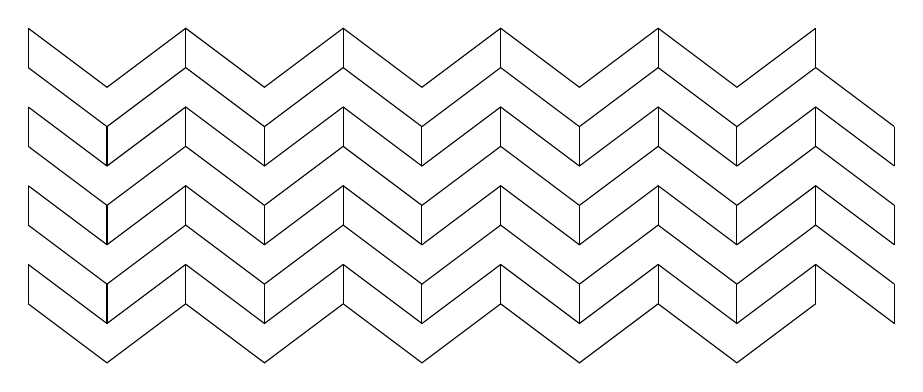
\begin{tikzpicture}[scale=1]


\draw  (0,0) -- (1,-0.75) -- (2,0) -- (3,-0.75) -- (4, 0) -- (5,-0.75)-- (6, 0) -- (7,-0.75)-- (8, 0) -- (9,-0.75)-- (10, 0);
\draw  (0,0.5) -- (1,-0.25) -- (2,0.5) -- (3,-0.25) -- (4, 0.5) -- (5,-0.25)-- (6, 0.5) -- (7,-0.25)-- (8, 0.5) -- (9,-0.25)-- (10, 0.5) -- (11,-0.25);
\draw  (0,1) -- (1,0.25) -- (2,1) -- (3,0.25) -- (4, 1) -- (5,0.25)-- (6, 1) -- (7,0.25)-- (8, 1) -- (9,0.25)-- (10, 1) -- (11,0.25);
\draw  (0,1.5) -- (1,0.75) -- (2,1.5) -- (3,0.75) -- (4, 1.5) -- (5,0.75)-- (6, 1.5) -- (7,0.75)-- (8, 1.5) -- (9,0.75)-- (10, 1.5) -- (11,0.75);
\draw  (0,2) -- (1,1.25) -- (2,2) -- (3,1.25) -- (4, 2) -- (5,1.25)-- (6, 2) -- (7,1.25)-- (8, 2) -- (9,1.25)-- (10, 2) -- (11,1.25);
\draw  (0,2.5) -- (1,1.75) -- (2,2.5) -- (3,1.75) -- (4, 2.5) -- (5,1.75)-- (6, 2.5) -- (7,1.75)-- (8, 2.5) -- (9,1.75)-- (10, 2.5) -- (11,1.75);
\draw  (0,3) -- (1,2.25) -- (2,3) -- (3,2.25) -- (4, 3) -- (5,2.25)-- (6, 3) -- (7,2.25)-- (8, 3) -- (9,2.25)-- (10, 3) -- (11,2.25);
\draw  (0,3.5) -- (1,2.75) -- (2,3.5) -- (3,2.75) -- (4, 3.5) -- (5,2.75)-- (6, 3.5) -- (7,2.75)-- (8,3.5) -- (9,2.75)-- (10, 3.5);


\draw (0,0) -- (0,0.5)   (0,1) -- (0,1.5)  (0,2) -- (0,2.5)  (0,3) -- (0,3.5);
\draw (2,0) -- (2,0.5)   (2,1) -- (2,1.5)  (2,2) -- (2,2.5)  (2,3) -- (2,3.5);
\draw (4,0) -- (4,0.5)   (4,1) -- (4,1.5)  (4,2) -- (4,2.5)  (4,3) -- (4,3.5);
\draw (6,0) -- (6,0.5)   (6,1) -- (6,1.5)  (6,2) -- (6,2.5)  (6,3) -- (6,3.5);
\draw (8,0) -- (8,0.5)   (8,1) -- (8,1.5)  (8,2) -- (8,2.5)  (8,3) -- (8,3.5);
\draw (10,0) -- (10,0.5)   (10,1) -- (10,1.5)  (10,2) -- (10,2.5)  (10,3) -- (10,3.5);

\draw (1,-0.25)  -- (1,0.25)  (1,0.75) -- (1,1.25) (1,1.75) -- (1,2.25);
\draw (3,-0.25) --  (3,0.25)  (3,0.75) -- (3,1.25) (3,1.75) -- (3,2.25);
\draw (5,-0.25)  -- (5,0.25)  (5,0.75) --  (5,1.25)  (5,1.75) -- (5,2.25);
\draw (7,-0.25) --  (7,0.25) (7,0.75)  --(7,1.25) (7,1.75) -- (7,2.25);
\draw (9,-0.25)  -- (9,0.25) (9,0.75) -- (9,1.25) (9,1.75)  --(9,2.25);
\draw (11,-0.25)  -- (11,0.25) (11,0.75) -- (11,1.25)  (11,1.75) -- (11,2.25);




\end{tikzpicture}
\end{center}
\caption{A wallpaper pattern in ${\mathbb R}^2$}
\label{Wallpaper}
\end{figure}
 
 
 
\subsection*{The Wallpaper Groups}
 
 
 
Suppose that we wish to study wallpaper patterns in the plane or
crystals in three dimensions. Wallpaper patterns are simply repeating
patterns in the plane (Figure~\ref{Wallpaper}). The analogs of
wallpaper patterns in ${\mathbb R}^3$ are crystals, which we can think of
as repeating patterns of molecules in three dimensions
(Figure~\ref{Crystals}). The mathematical equivalent of a wallpaper or
crystal pattern is called a  lattice. 
 
 
 
\begin{figure}[hbt]


%Replaced figure with tikz figure - TWJ 6/11/2010
\begin{center}
\tikzpreface{matrix_crystal_R3}
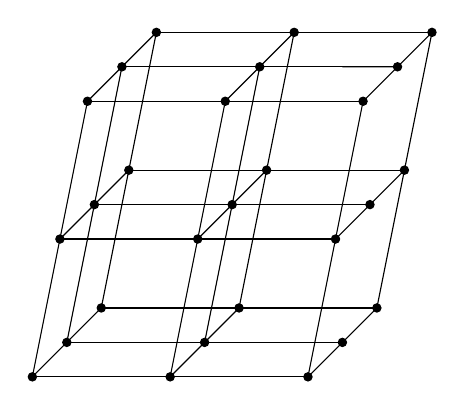
\begin{tikzpicture}[scale=1.75]


\draw  (0,0) -- (2,0)  (0.25,0.25) -- (2.25,0.25)  (0.5,0.5) -- (2.5,0.5);

\foreach \x in {0,1,2} \filldraw[fill=black, draw=black] (\x,0) circle (0.03);
\foreach \x in {0.25,1.25,2.25} \filldraw[fill=black, draw=black] (\x,0.25) circle (0.03);
\foreach \x in {0.5,1.5,2.5} \filldraw[fill=black, draw=black] (\x,0.5) circle (0.03);

\draw  (0.2,1) -- (2.2,1)  (0.45,1.25) -- (2.45,1.25)  (0.7,1.5) -- (2.7,1.5) ;

\foreach \x in {0.2,1.2,2.2} \filldraw[fill=black, draw=black] (\x,1) circle (0.03);
\foreach \x in {0.45,1.45,2.45} \filldraw[fill=black, draw=black] (\x,1.25) circle (0.03);
\foreach \x in {0.7,1.7,2.7} \filldraw[fill=black, draw=black] (\x,1.5) circle (0.03);

\draw  (0.4,2) -- (2.4,2)  (0.65,2.25) -- (2.65,2.25)  (0.9,2.5) -- (2.9,2.5) ;

\foreach \x in {0.4,1.4,2.4} \filldraw[fill=black, draw=black] (\x,2) circle (0.03);
\foreach \x in {0.65,1.65,2.65} \filldraw[fill=black, draw=black] (\x,2.25) circle (0.03);
\foreach \x in {0.9,1.9,2.9} \filldraw[fill=black, draw=black] (\x,2.5) circle (0.03);

\draw (0,0) -- (0.4,2)  (0.25,0.25) -- (0.65,2.25) (0.5,0.5) -- (0.9,2.5);
\draw (1,0) -- (1.4,2)  (1.25,0.25) -- (1.65,2.25) (1.5,0.5) -- (1.9,2.5);
\draw (2,0) -- (2.4,2)  (2.25,2.25) -- (2.65,2.25) (2.5,0.5) -- (2.9,2.5);

\draw (0,0) -- (0.5,0.5)  (1,0) -- (1.5,0.5)  (2,0) -- (2.5,0.5);

\draw  (0.2,1) -- (0.7,1.5)  (1.2,1) -- (1.7,1.5)  (2.2,1) -- (2.7,1.5);

\draw  (0.4,2) -- (0.9,2.5) (1.4,2) -- (1.9,2.5)   (2.4,2) -- (2.9,2.5);


\end{tikzpicture}
\end{center}
\caption{A crystal structure in ${\mathbb R}^3$}
\label{Crystals}
\end{figure}
 
 

Let us examine wallpaper patterns in the plane a
little more closely. Suppose that ${\mathbf x}$ and ${\mathbf y}$ are
linearly independent vectors in ${\mathbb R}^2$; that is, one vector
cannot be a scalar multiple of the other. A \boldemph{
lattice}\index{Lattice of points} of ${\mathbf x}$ and ${\mathbf y}$ is
the set of all linear combinations $m {\mathbf x} + n {\mathbf y}$, where
$m$ and $n$ are integers. The vectors ${\mathbf x}$ and ${\mathbf y}$ are
said to be a \boldemph{basis}\index{Basis of a lattice} for the lattice.
 
 
\begin{figure}[htb]


%Replaced figure with tikz figure - TWJ 6/11/2010
\begin{center}
\tikzpreface{matrix_lattice_R2}
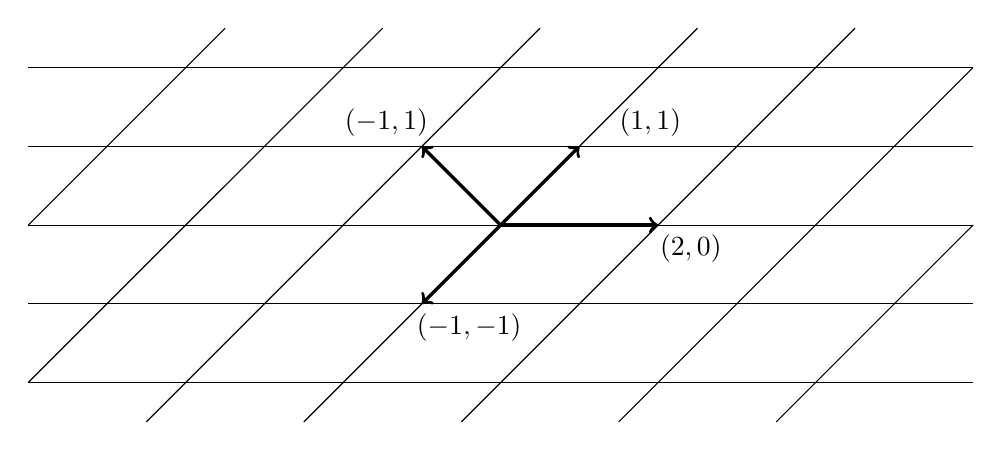
\begin{tikzpicture}[scale=1]



\foreach \x in {-2, -1, 0, 1, 2} \draw  (-6,\x) -- (6,\x); 

\draw (3.5,-2.5) -- (6,0);
\draw (1.5,-2.5) -- (6,2);
\draw (-0.5,-2.5) -- (4.5,2.5);
\draw (-2.5,-2.5) -- (2.5,2.5);
\draw (-4.5,-2.5) -- (0.5,2.5);
\draw (-6,-2) -- (-1.5,2.5);
\draw (-6,0) -- (-3.5,2.5);

\draw [->, very thick, black]  (0,0) -- (2,0);
\draw [->, very thick, black]  (0,0) -- (1,1);
\draw [->, very thick, black]  (0,0) -- (-1,1);
\draw [->, very thick, black]  (0,0) -- (-1,-1); 

\node [right] at (1.9,-0.3) {$(2,0)$};
\node [above] at (1.9,1) {$(1,1)$};
\node [above] at (-1.45,1) {$(-1,1)$};
\node [below] at (-0.4,-1) {$(-1,-1)$};

\end{tikzpicture}
\end{center}
\caption{A lattice in  ${\mathbb R}^2$}
\label{lattice}
\end{figure}
 
 
Notice that a lattice can have several bases. For example, the vectors
$(1,1)^{\rm t}$ and $(2,0)^{\rm t}$ have the  same lattice as the
vectors $(-1, 1)^{\rm t}$ and $(-1, -1)^{\rm t}$
(Figure~\ref{lattice}). However, any lattice is completely determined
by a basis. Given two bases for the same lattice, say $\{ {\mathbf x}_1,
{\mathbf x}_2 \}$ and $\{ {\mathbf y}_1, {\mathbf y}_2 \}$, we can write 
\begin{align*}
{\mathbf y}_1 & = \alpha_1  {\mathbf x}_1 + \alpha_2 {\mathbf x}_2 \\
{\mathbf y}_2 & = \beta_1  {\mathbf x}_1 + \beta_2 {\mathbf x}_2,
\end{align*}
where $\alpha_1$, $\alpha_2$, $\beta_1$, and $\beta_2$ are integers.
The matrix corresponding to this transformation is 
\[
U
=
\begin{pmatrix}
\alpha_1 & \alpha_2 \\
\beta_1 & \beta_2
\end{pmatrix}.
\]
If we wish to give ${\mathbf x}_1$ and ${\mathbf x}_2$ in terms of ${\mathbf
y}_1$ and ${\mathbf y}_2$, we need only calculate $U^{-1}$; that is, 
\[
U^{-1}
\begin{pmatrix}
{\mathbf y}_1 \\ {\mathbf y}_2
\end{pmatrix}
=
\begin{pmatrix}
{\mathbf x}_1 \\ {\mathbf x}_2
\end{pmatrix}.
\]
Since $U$ has integer entries, $U^{-1}$ must also have integer
entries; hence the determinants of both $U$ and $U^{-1}$ must be
integers. Because $U U^{-1} = I$,  
\[
\det(U U^{-1}) =\det(U) \det( U^{-1}) = 1;
\]
consequently, $\det(U) = \pm 1$. A matrix with determinant $\pm 1$ and
integer entries is called \boldemph{unimodular}\index{Matrix!unimodular}.
For example, the matrix 
\[
\begin{pmatrix}
3 & 1 \\
5 & 2
\end{pmatrix}
\]
is unimodular. It should be clear that there is a minimum length for
vectors in a lattice.  
 
 
We can classify lattices by studying their symmetry groups. The
symmetry group of a lattice is the subgroup of $E(2)$ that maps the
lattice to itself. We consider two lattices in ${\mathbb R}^2$ to be
equivalent if they have the same symmetry group.  Similarly,
classification of crystals in ${\mathbb R}^3$ is accomplished by
associating a symmetry group, called a \boldemph{space group}, with each
type of crystal\index{Group!space}. Two lattices are considered
different if their space groups are not the same.  The natural
question that now arises is how many space groups exist. 
 
 
A space group is composed of two parts: a \boldemph{translation
subgroup}\index{Subgroup!translation} and a \boldemph{point
group}\index{Group!point}.  The translation subgroup is an infinite
abelian subgroup of the space group made up of the translational
symmetries of the crystal; the point group is a finite group 
consisting  of rotations and reflections of the crystal about a point.
More specifically, a space group is a subgroup of $G \subset E(2)$
whose translations are a set of the form $\{ (I, t) : t \in L \}$,
where $L$ is a lattice. Space groups are, of course, infinite. Using
geometric arguments, we can prove the following theorem (see [5] or [6]).
 
 
 
 
\begin{theorem}
Every translation group in ${\mathbb R}^2$ is isomorphic to ${\mathbb Z}
\times {\mathbb Z}$.
\end{theorem}
 
 
\begin{figure}[bht]

\begin{center}
\tikzpreface{matrix_lattices_R2}
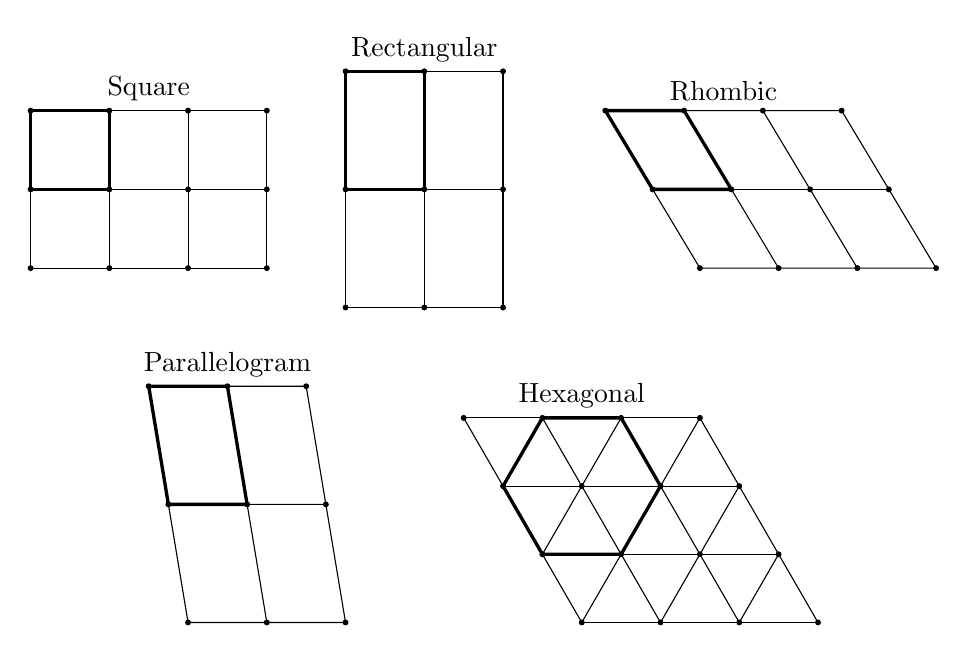
\begin{tikzpicture}[scale=1] %Replaced figure with tikz figure - TWJ 6/14/2010

\node [above] at (0,7) {Rectangular};
\draw (-1,4) -- (1,4) -- (1,7) -- (-1,7) -- cycle;
\draw  (0,4) -- (0,7)  (-1,5.5) -- (1,5.5);
\draw [very thick] (-1,5.5) -- (-1,7) -- (0,7) -- (0,5.5) -- cycle;
\foreach \x in {-1,0,1} \filldraw[fill=black, draw=black] (\x,4) circle (0.03);
\foreach \x in {-1,0,1} \filldraw[fill=black, draw=black] (\x,5.5) circle (0.03);
\foreach \x in {-1,0,1} \filldraw[fill=black, draw=black] (\x,7) circle (0.03);

\node [above] at (-3.5,6.5) {Square};
\draw (-2,4.5) -- (-5,4.5) -- (-5,6.5) -- (-2,6.5) -- cycle;
\draw  (-2,5.5) -- (-5,5.5)  (-3,4.5) -- (-3,6.5) (-4,4.5) -- (-4,6.5);
\draw [very thick] (-5,5.5) -- (-5,6.5) -- (-4,6.5) -- (-4,5.5) -- cycle;
\foreach \x in {-2, -3, -4, -5} \filldraw[fill=black, draw=black] (\x,4.5) circle (0.03);
\foreach \x in {-2, -3, -4, -5} \filldraw[fill=black, draw=black] (\x,5.5) circle (0.03);
\foreach \x in {-2, -3, -4, -5} \filldraw[fill=black, draw=black] (\x,6.5) circle (0.03);

\node [above] at (3.8,6.5) {Rhombic};
\draw (3.5,4.5)   -- (6.5,4.5) -- (5.3,6.5) -- (2.3,6.5) -- cycle;
\draw (2.9,5.5) -- (5.9,5.5);
\draw (4.5,4.5) -- (3.3,6.5);
\draw  (5.5,4.5) -- (4.3,6.5);
\draw [very thick] (2.3,6.5) -- (3.3,6.5) -- (3.9,5.5) -- (2.9,5.5) -- cycle;
\foreach \x in {3.5,4.5,5.5,6.5} \filldraw[fill=black, draw=black] (\x,4.5) circle (0.03);
\foreach \x in {2.9,3.9,4.9,5.9} \filldraw[fill=black, draw=black] (\x,5.5) circle (0.03);
\foreach \x in {2.3,3.3,4.3,5.3} \filldraw[fill=black, draw=black] (\x,6.5) circle (0.03);

\node [above] at (-2.5,3) {Parallelogram};
\draw (-1,0) -- (-3,0) -- (-3.5,3) -- (-1.5,3) -- cycle;
\draw  (-2,0) -- (-2.5,3)  (-3.25,1.5) -- (-1.25,1.5);
\draw [very thick] (-3.25,1.5) -- (-3.5,3) -- (-2.5,3) -- (-2.25,1.5) -- cycle;
\foreach \x in {-1,-2,-3} \filldraw[fill=black, draw=black] (\x,0) circle (0.03);
\foreach \x in {-1.25,-2.25,-3.25} \filldraw[fill=black, draw=black] (\x,1.5) circle (0.03);
\foreach \x in {-1.5,-2.5,-3.5} \filldraw[fill=black, draw=black] (\x,3) circle (0.03);

\node [above] at (2,2.6) {Hexagonal}; %Couldn't figure out an elegant way to do the hexagonal lattice - TWJ 6/14/2010
\draw (2,0) -- (5,0);
\draw (1.5,0.866) -- (4.5,0.866);
\draw (1,1.732) -- (4,1.732);
\draw (0.5,2.598) -- (3.5,2.598);
\draw (2,0) -- (0.5,2.598);
\draw (3,0) -- (1.5,2.598);
\draw (4,0) -- (2.5,2.598);
\draw (5,0) -- (3.5,2.598);
\draw (2,0) -- (3.5,2.598);
\draw (3,0) -- (4,1.732);
\draw (4,0) -- (4.5,0.866);
\draw (1.5,0.866) -- (2.5,2.598);
\draw (1,1.732) -- (1.5,2.598);
\draw [very thick] (1.5,0.866) -- (1,1.732) -- (1.5,2.598) -- (2.5,2.598) -- (3,1.732) --  (2.5,0.866) -- cycle;
\foreach \x in {2,3,4,5} \filldraw[fill=black, draw=black] (\x,0) circle (0.03);
\foreach \x in {1.5,2.5,3.5,4.5} \filldraw[fill=black, draw=black] (\x,0.866) circle (0.03);
\foreach \x in {1,2,3,4} \filldraw[fill=black, draw=black] (\x,1.732) circle (0.03);
\foreach \x in {0.5, 1.5,2.5,3.5} \filldraw[fill=black, draw=black] (\x,2.598) circle (0.03);

\end{tikzpicture}
\end{center}
\caption{Types of lattices in  ${\mathbb R}^2$}
\label{Types}
\end{figure}
 
 
The point group of $G$ is $G_0 = \{A : (A,b) \in G \text{ for some }
b \}$. In particular, $G_0$ must be a subgroup of $O(2)$. Suppose
that ${\mathbf x}$ is a vector in a lattice $L$ with space group $G$,
translation group $H$, and point group $G_0$. For any element $(A,
{\mathbf y})$ in $G$,   
\begin{align*}
(A, {\mathbf y}) (I, {\mathbf x}) (A, {\mathbf y})^{-1}
& =
(A,A {\mathbf x} + {\mathbf y}) (A^{-1},-A^{-1} {\mathbf y}) \\
& =
(A A^{-1},-A A^{-1} {\mathbf y} + A {\mathbf x} + {\mathbf y}) \\
& =
(I, A {\mathbf x});
\end{align*}
hence, $(I, A {\mathbf x})$ is in the translation group of $G$. More
specifically, $A {\mathbf x}$ must be in the lattice $L$. It is
important to note that $G_0$ is not usually a subgroup of the space
group $G$; however, if $T$ is the translation subgroup of $G$, then
$G/T \cong G_0$. The proof of the following theorem can be found in
[2], [5], or~[6].
 
 
 
\begin{theorem}
The point group in the wallpaper groups is isomorphic to ${\mathbb Z}_n$
or $D_n$, where $n = 1, 2, 3, 4, 6$. 
\end{theorem}
 
 
To answer the question of how the point groups and the translation
groups can be combined, we must look at the different types of
lattices. Lattices can be classified by the structure of a single
lattice cell. The possible cell shapes are parallelogram, rectangular,
square, rhombic, and hexagonal (Figure~\ref{Types}). The wallpaper
groups can now be classified according to the types of reflections
that occur in each group: these are ordinarily reflections, glide
reflections, both, or none.
 
 
 
\begin{table}[htb]
\caption{The 17 wallpaper groups}{\small
\begin{center}
\begin{tabular}{|l|l|l|l|}
\hline
Notation and &             &              & Reflections  \\
Space Groups & Point Group & Lattice Type & or Glide Reflections? \\
\hline
p1 & ${\mathbb Z}_1$ & parallelogram & none \\
p2 & ${\mathbb Z}_2$ & parallelogram & none \\
p3 & ${\mathbb Z}_3$ & hexagonal & none \\
p4 & ${\mathbb Z}_4$ & square & none \\
p6 & ${\mathbb Z}_6$ & hexagonal & none \\
pm & $D_1$ & rectangular & reflections \\
pg & $D_1$ & rectangular & glide reflections\\
cm & $D_1$ & rhombic & both \\
pmm & $D_2$ & rectangular & reflections \\
pmg & $D_2$ & rectangular & glide reflections \\
pgg & $D_2$ & rectangular & both \\
c2mm & $D_2$ & rhombic & both \\
p3m1, p31m & $D_3$ & hexagonal & both \\
p4m, p4g & $D_4$ & square & both \\
p6m & $D_6$ & hexagonal & both \\
\hline
\end{tabular} \label{table:wallpaper}
\end{center}
}
\end{table}
 
 
\begin{theorem}
There are exactly 17 wallpaper groups.
\end{theorem}
 
 
\begin{figure}[htb]


\begin{center}
\tikzpreface{matrix_p4m_p4g}
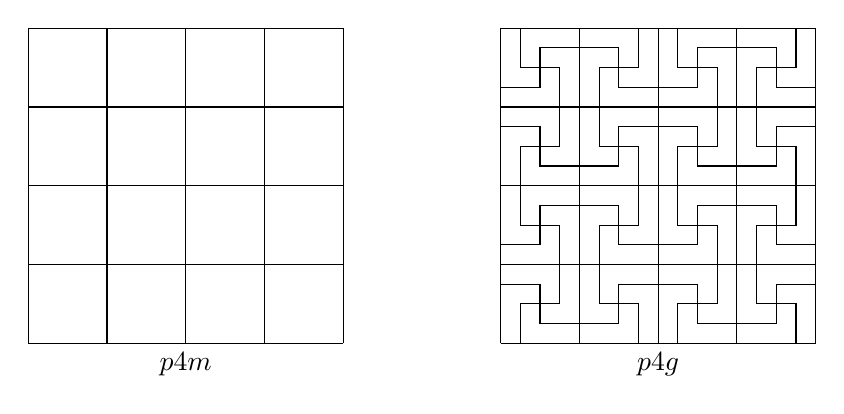
\begin{tikzpicture}[scale=1] %Replaced figure with tikz figure - TWJ 6/14/2010

\draw[step=1] (-5,0) grid (-1,4);
\node [below] at (-3,0) {$p4m$};

\draw[step=1] (1,0) grid (5,4);
\node [below] at (3,0) {$p4g$};
\draw (1.25,0) -- (1.25,0.5) -- (1.75,0.5) -- (1.75,1.5) -- (1.25,1.5) -- (1.25,2.5) -- (1.75,2.5) -- (1.75,3.5) -- (1.25,3.5) -- (1.25,4);
\draw  (2.75,0) -- (2.75,0.5) -- (2.25,0.5) -- (2.25,1.5) -- (2.75,1.5) -- (2.75,2.5) -- (2.25,2.5) -- (2.25,3.5) -- (2.75,3.5) -- (2.75,4);
\draw   (3.25,0) -- (3.25,0.5) -- (3.75,0.5) -- (3.75,1.5) -- (3.25,1.5) -- (3.25,2.5) -- (3.75,2.5) -- (3.75,3.5) -- (3.25,3.5) -- (3.25,4);
\draw   (4.75,0) -- (4.75,0.5) -- (4.25,0.5) -- (4.25,1.5) -- (4.75,1.5) -- (4.75,2.5) -- (4.25,2.5) -- (4.25,3.5) -- (4.75,3.5) -- (4.75,4);

\draw  (1,0.75) -- (1.5,0.75) -- (1.5,0.25) -- (2.5,0.25) -- (2.5,0.75) -- (3.5,0.75) -- (3.5,0.25) -- (4.5,0.25) -- (4.5,0.75) -- (5, 0.75);
\draw  (1,1.25) -- (1.5,1.25) -- (1.5,1.75) -- (2.5,1.75) -- (2.5,1.25) -- (3.5,1.25) -- (3.5,1.75) -- (4.5,1.75) -- (4.5,1.25) -- (5, 1.25);

\draw  (1,2.75) -- (1.5,2.75) -- (1.5,2.25) -- (2.5,2.25) -- (2.5,2.75) -- (3.5,2.75) -- (3.5,2.25) -- (4.5,2.25) -- (4.5,2.75) -- (5, 2.75);
\draw (1,3.25) -- (1.5,3.25) -- (1.5,3.75) -- (2.5,3.75) -- (2.5,3.25) -- (3.5,3.25) -- (3.5,3.75) -- (4.5,3.75) -- (4.5,3.25) -- (5, 3.25);


\end{tikzpicture}
\end{center}
\caption{The wallpaper groups p4m and  p4g}
\label{p4m}
\end{figure}
 
 
 
The 17 wallpaper groups are listed in Table~\ref{table:wallpaper}. The groups p3m1 and
p31m can be distinguished by whether or not all of their threefold
centers lie on the reflection axes: those of p3m1 must, whereas those
of p31m may not. Similarly, the fourfold centers of p4m must lie on
the reflection axes whereas those of p4g need not (Figure~\ref{p4m}).
The complete proof of this theorem can be found in several of the
references at the end of this chapter, including [5], [6], [10],
and~[11]. 
 
 
 
\histhead
 
 
\noindent{\small \histf
Symmetry groups have intrigued mathematicians for a long time.
Leonardo da Vinci was probably the first person to know all of the
point groups.  At the International Congress of Mathematicians in
1900, David Hilbert\index{Hilbert, David} gave a now-famous address
outlining 23 problems to guide mathematics in the twentieth
century.  Hilbert's eighteenth problem asked whether or not
crystallographic groups in $n$ dimensions were always finite.  In
1910, L.~Bieberbach\index{Bieberbach, L.} proved that crystallographic
groups are finite in every dimension.  Finding out how many of these
groups there are in each dimension is another matter. In ${\mathbb R}^3$
there are 230 different space groups; in ${\mathbb R}^4$ there are 4783.
No one has been able to compute the number of space groups for ${\mathbb
R}^5$ and beyond. It is interesting to note that the crystallographic
groups were found mathematically for ${\mathbb R}^3$ before the 230
different types of crystals were actually discovered in nature.
\histbox
}
 
 
 
\markright{EXERCISES}
\section*{Exercises}
\exrule
 
 
{\small
\begin{enumerate}
 
 
 
\item
Prove the identity
\[
\langle {\mathbf x}, {\mathbf y} \rangle = \frac{1}{2}
\left[
\|{\mathbf x} + {\mathbf y}\|^2 - \|{\mathbf x}\|^2 - \| {\mathbf y}\|^2
\right].
\]
 
 
\item
Show that $O(n)$ is a group.
 
 
\item
Prove that the following matrices are orthogonal. Are any of
these matrices in $SO(n)$?
\begin{multicols}{2}
\begin{enumerate}

\item
\[
\begin{pmatrix}
1/\sqrt{2} & -1/\sqrt{2} \\
1/\sqrt{2} & 1/\sqrt{2}
\end{pmatrix}
\]

\item
\[
\begin{pmatrix}
1 / \sqrt{5} & 2 / \sqrt{5} \\
- 2 /\sqrt{5} & 1/ \sqrt{5}
\end{pmatrix}
\]

\item
\[
\begin{pmatrix}
4/ \sqrt{5} & 0 & 3 / \sqrt{5} \\
-3 / \sqrt{5} & 0 & 4 / \sqrt{5} \\
0 & -1 & 0
\end{pmatrix}
\]

\item
\[
\begin{pmatrix}
1/3 & 2/3 & - 2/3 \\
- 2/3 & 2/3 & 1/3 \\
-2/3 & 1/3 & 2/3
\end{pmatrix}
\]


\end{enumerate}
\end{multicols}
 

 
\item %%%%%%%%%%%%%%%%%%%%%%
Determine the symmetry group of each of the figures in
Figure~\ref{Determine}. 
\begin{figure}[htb]

\begin{center}
\tikzpreface{matrix_group_exercise}
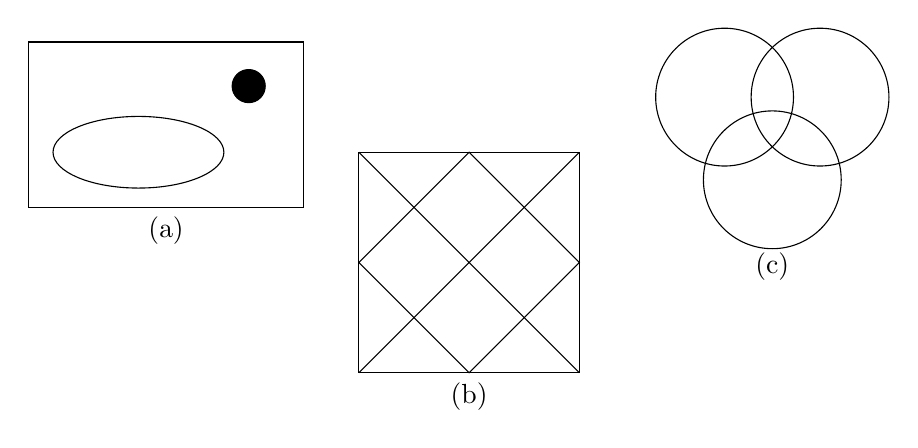
\begin{tikzpicture}[scale=0.7] %Replaced figure with tikz figure - TWJ 6/14/2010

\draw (-2,0) -- (2,0) -- (2,4) -- (-2,4) -- cycle;
\draw (0,0) -- (2,2) -- (0,4) -- (-2,2) -- cycle;
\draw (-2,0) -- (2,4) (2,0) -- (-2,4);
\node [below] at (0,0) {(b)};

\draw (-3,3) -- (-8,3) -- (-8,6) -- (-3,6) -- cycle;
\draw (-6,4) ellipse (1.55 and 0.65);
\filldraw[fill=black, draw=black] (-4,5.2) circle (0.3);
\node [below] at (-5.5,3) {(a)};



\draw (5.5,4.5)  +(270:1) circle (1.25);
\draw (5.5,4.5)  +(30:1) circle (1.25);
\draw (5.5,4.5)  +(150:1) circle (1.25);
\node [below] at (5.5,2.35) {(c)};


\end{tikzpicture}
\end{center}
\caption{}
\label{Determine}
\end{figure}
 
 
\item
Let ${\mathbf x}$, ${\mathbf y}$, and ${\mathbf w}$ be vectors in ${\mathbb
R}^n$ and $\alpha \in {\mathbb R}$.  Prove each of the following
properties of inner products.
\begin{enumerate}
 
 \item
$\langle {\mathbf x}, {\mathbf y} \rangle = \langle {\mathbf y}, {\mathbf x}
\rangle$. 
 
 \item
$\langle {\mathbf x}, {\mathbf y} + {\mathbf w} \rangle = \langle
{\mathbf x}, {\mathbf y} \rangle + \langle {\mathbf x}, {\mathbf w}
\rangle$.
 
 \item
$\langle \alpha {\mathbf x}, {\mathbf y} \rangle = \langle
{\mathbf x}, \alpha {\mathbf y} \rangle = \alpha \langle  {\mathbf
x}, {\mathbf y} \rangle$.
 
 \item
$\langle {\mathbf x}, {\mathbf x} \rangle \geq 0$ with equality exactly
when ${\mathbf x} = 0$. 
 
 \item
If $\langle {\mathbf x}, {\mathbf y} \rangle = 0$  for all ${\mathbf x}$ in
${\mathbb R}^n$, then ${\mathbf y} = 0$. 
 
\end{enumerate}
 
 
\item \label{matrix:En_group_exercise}
Verify that
\[
E(n)
=
\{(A, {\mathbf x}) : A \in O(n) \mbox{ and } {\mathbf x} \in
{\mathbb R}^n \}
\]
is a group.
 
 
\item
Prove that $\{ (2,1), (1,1) \}$  and $\{ ( 12, 5), ( 7, 3) \}$ are bases
for the same lattice. 
 
 
\item
Let $G$ be a subgroup of $E(2)$ and suppose that $T$ is the
translation subgroup of $G$.  Prove that the point group of $G$ is
isomorphic to $G/T$. 
 
 
\item
Let $A \in SL_2({\mathbb R})$ and suppose that the vectors ${\mathbf x}$
and ${\mathbf y}$ form two sides of a parallelogram in ${\mathbb R}^2$.
Prove that the area of this parallelogram is the same as the area of
the parallelogram with sides $A{\mathbf x}$ and $A{\mathbf y}$. 
 
 
\item
Prove that $SO(n)$ is a normal subgroup of $O(n)$.
 
 
\item
Show that any isometry $f$ in ${\mathbb R}^n$ is a one-to-one map.
 
 
\item
Show that an element in $E(2)$ of the form $(A, {\mathbf x})$,
where ${\mathbf x} \neq 0$, has infinite order.
 
 
\item
Prove or disprove: There exists an infinite abelian subgroup of 
$O(n)$.
 
 
\item
Let ${\mathbf x} = (x_1, x_2)$ be a point on the unit circle in ${\mathbb
R}^2$; that is, $x_1^2 + x_2^2 = 1$. If $A \in O(2)$, show that $A
{\mathbf x}$ is also a point on the unit circle. 
 
 
 
\item
Let $G$ be a group with a subgroup $H$ (not necessarily normal) and a
normal subgroup $N$. Then $G$ is a \boldemph{semidirect
product}\index{Semidirect product} of $N$ by $H$ if  
\begin{itemize}
 
 \item
$H \cap N = \{ id \}$;
 
 \item
$HN=G$.
 
\end{itemize}
Show that each of the following is true.
\begin{enumerate}
 
 \item
$S_3$ is the semidirect product of $A_3$ by $H = \{(1), (12) \}$.
 
 \item
The quaternion group, $Q_8$, cannot be written as a semidirect product. 
 
 \item
$E(2)$ is the semidirect product of $O(2)$ by $H$, where $H$ consists
of all translations in ${\mathbb R}^2$. 
 
\end{enumerate}
 
 
 
\item
Determine which of the 17 wallpaper groups preserves the symmetry of
the pattern in Figure~\ref{Wallpaper}.  
 
\begin{figure}[htb]

\begin{center}
\tikzpreface{matrix_wallpaper_exercise}
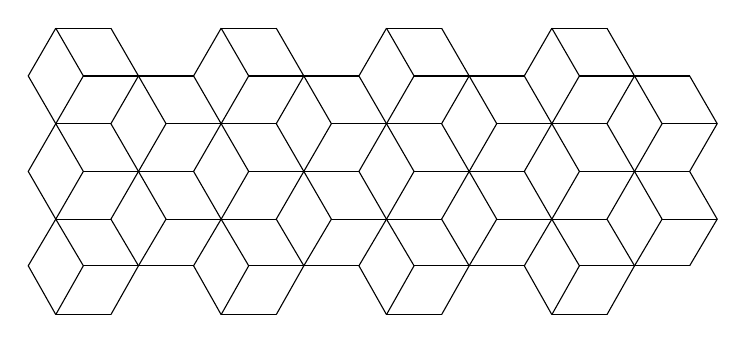
\begin{tikzpicture}[scale=0.7] %Replaced figure with tikz figure - TWJ 6/14/2010

\draw (0.5,0) -- (1.5,0)  (3.5,0) -- (4.5,0) (6.5,0) -- (7.5,0) (9.5,0) -- (10.5,0);
\draw (1,0.886) -- (3,0.886) (4,0.886) -- (6,0.886) (7,0.886) -- (9,0.886) (10,0.886) -- (12,0.886);
\draw (0.5,1.732) -- (1.5,1.732)  (2.5,1.732) -- (4.5,1.732) (5.5,1.732) -- (7.5,1.732) (8.5,1.732) -- (10.5,1.732) (11.5,1.732) -- (12.5,1.732);
\draw (1,2.598) -- (3,2.598) (4,2.598) -- (6,2.598) (7,2.598) -- (9,2.598) (10,2.598) -- (12,2.598);
\draw (0.5,3.464) -- (1.5,3.464)  (2.5,3.464) -- (4.5,3.464) (5.5,3.464) -- (7.5,3.464) (8.5,3.464) -- (10.5,3.464) (11.5,3.464) -- (12.5,3.464);
\draw (1,4.33) -- (3,4.33) (4,4.33) -- (6,4.33) (7,4.33) -- (9,4.33) (10,4.33) -- (12,4.33);
\draw (0.5,5.196) -- (1.5,5.196)  (3.5,5.196) -- (4.5,5.196) (6.5,5.196) -- (7.5,5.196) (9.5,5.196) -- (10.5,5.196);

\draw (0.5,0) -- (0,0.886) -- (0.5,1.732) -- (0,2.598) -- (0.5,3.464) -- (0,4.33) -- (0.5,5.196);
\draw (0.5,0) -- (1,0.886) -- (0.5,1.732) -- (1,2.598) -- (0.5,3.464) -- (1,4.33) -- (0.5,5.196);
\draw (1.5,0) -- (2,0.886) -- (1.5,1.732) -- (2,2.598) -- (1.5,3.464) -- (2,4.33) -- (1.5,5.196);
\draw (2,0.886) -- (2.5,1.732) -- (2,2.598) -- (2.5,3.464) -- (2,4.33);
\draw (3,0.886) -- (3.5,1.732) -- (3,2.598) -- (3.5,3.464) -- (3,4.33);
\draw (3.5,0) -- (3,0.886) (3,4.33) -- (3.5,5.196);
\draw (3.5,0) -- (4,0.886) -- (3.5,1.732) -- (4,2.598) -- (3.5,3.464) -- (4,4.33) -- (3.5,5.196);
\draw (4.5,0) -- (5,0.886) -- (4.5,1.732) -- (5,2.598) -- (4.5,3.464) -- (5,4.33) -- (4.5,5.196);
\draw (5,0.886) -- (5.5,1.732) -- (5,2.598) -- (5.5,3.464) -- (5,4.33);
\draw (6.5,0) -- (6,0.886) -- (6.5,1.732) -- (6,2.598) -- (6.5,3.464) -- (6,4.33) -- (6.5,5.196);
\draw (6.5,0) -- (7,0.886) -- (6.5,1.732) -- (7,2.598) -- (6.5,3.464) -- (7,4.33) -- (6.5,5.196);
\draw (7.5,0) -- (8,0.886) -- (7.5,1.732) -- (8,2.598) -- (7.5,3.464) -- (8,4.33) -- (7.5,5.196);
\draw (8,0.886) -- (8.5,1.732) -- (8,2.598) -- (8.5,3.464) -- (8,4.33);
\draw (9.5,0) -- (9,0.886) -- (9.5,1.732) -- (9,2.598) -- (9.5,3.464) -- (9,4.33) -- (9.5,5.196);
\draw (9.5,0) -- (10,0.886) -- (9.5,1.732) -- (10,2.598) -- (9.5,3.464) -- (10,4.33) -- (9.5,5.196);
\draw (10.5,0) -- (11,0.886) -- (10.5,1.732) -- (11,2.598) -- (10.5,3.464) -- (11,4.33) -- (10.5,5.196);
\draw (11,0.886) -- (11.5,1.732) -- (11,2.598) -- (11.5,3.464) -- (11,4.33);
\draw (12,0.886) -- (12.5,1.732) -- (12,2.598) -- (12.5,3.464) -- (12,4.33);



\end{tikzpicture}
\end{center}
\caption{}
\label{For17}
\end{figure}
 
\item
Determine which of the 17 wallpaper groups preserves the symmetry of
the pattern in Figure~\ref{For17}.  
 
 
 
\item
Find the rotation group of a dodecahedron.
 
  
 
\item
For each of the 17 wallpaper groups, draw a wallpaper pattern having
that group as a symmetry group.  
 
\end{enumerate}
}
 
 
 
\subsection*{References and Suggested Readings}
 
 
 
{\small
\begin{itemize} %%References checked -- TWJ 6/14/2010
 
\item[\textbf{[1]}]
Coxeter, H. M. and Moser, W. O. J. \textit{Generators and
Relations for Discrete Groups}, 3rd ed. Springer-Verlag, New
York, 1972.
 
\item[\textbf{[2]}]
Grove, L. C. and Benson, C. T. \textit{Finite Reflection
Groups}. 2nd ed. Springer-Verlag, New York, 1985.
 
\item[\textbf{[3]}]
Hiller, H. ``Crystallography and Cohomology of Groups,''
\textit{American Mathematical Monthly} \textbf{93} (1986), 765--79.
 
\item[\textbf{[4]}]
Lockwood, E. H. and Macmillan, R. H. \textit{Geometric
Symmetry}. Cambridge University Press, Cambridge, 1978.
 
\item[\textbf{[5]}]
Mackiw, G. \textit{Applications of Abstract Algebra}. Wiley,
New York, 1985.
 
 
\item[\textbf{[6]}]
Martin,  G.  \textit{Transformation  Groups:  An Introduction to
Symmetry}.  Springer-Verlag, New York, 1982.
 
  
\item[\textbf{[7]}]
Milnor, J. ``Hilbert's Problem 18: On Crystallographic
Groups, Fundamental Domains, and Sphere Packing,'' {\it
Proceedings of Symposia in Pure Mathematics} \textbf{18},
American Mathematical Society, 1976.
 
\item[\textbf{[8]}]
Phillips, F. C. \textit{An Introduction to Crystallography}.
4th ed. Wiley, New York, 1971.
 
\item[\textbf{[9]}]
Rose, B. I. and Stafford, R. D. ``An Elementary Course in
Mathematical Symmetry,'' \textit{American Mathematical Monthly} \textbf{
88} (1980), 54--64.
 
 
\item[\textbf{[10]}]
Schattschneider, D. ``The Plane Symmetry Groups: Their
Recognition and Their Notation,'' \textit{American Mathematical 
Monthly} \textbf{85} (1978), 439--50.
 
 
\item[\textbf{[11]}]
Schwarzenberger, R. L. ``The 17 Plane Symmetry Groups,'' {\it
Mathematical  Gazette} \textbf{58} (1974), 123--31. 
 
 
\item[\textbf{[12]}]
Weyl, H. \textit{Symmetry}. Princeton University Press, Princeton, NJ,
1952. 
 
 
\end{itemize}
}
 
 
 
 
   %Groups of Symmetries
%%%%(c)
%%%%(c)  This file is a portion of the source for the textbook
%%%%(c)
%%%%(c)    Abstract Algebra: Theory and Applications
%%%%(c)    Copyright 1997 by Thomas W. Judson
%%%%(c)
%%%%(c)  See the file COPYING.txt for copying conditions
%%%%(c)
%%%%(c)
\chap{The Structure of  Groups}{struct}
 

The ultimate goal of group theory is to classify all groups up to
isomorphism; that is, given a particular group, we should be able to
match it up with a known group via an isomorphism. For example, we
have already proved that any finite cyclic group of order $n$ is
isomorphic to ${\mathbb Z}_n$; hence, we ``know'' all finite cyclic
groups. It is probably not reasonable to expect that we will ever know
all groups; however, we can often classify certain types of groups or
distinguish between groups in special cases.  

In this chapter we will characterize all finite abelian groups. We
shall also investigate groups with sequences of subgroups.  If a group
has a sequence of subgroups, say 
\[
G = H_n \supset H_{n-1} \supset \cdots \supset H_1 \supset H_0 = \{ e
\}, 
\]
where each subgroup $H_i$ is normal in $H_{i+1}$ and each of the
factor groups $H_{i+1}/H_i$ is abelian, then $G$ is a solvable group.
In addition to allowing us to distinguish between certain classes of
groups, solvable groups turn out to be central to the study of
solutions to polynomial equations.
 

\section{Finite Abelian Groups}

In our investigation of cyclic groups we found that every group of
prime order was isomorphic to ${\mathbb Z}_p$, where $p$ was a prime
number.  We also determined that ${\mathbb Z}_{mn} \cong {\mathbb Z}_m
\times {\mathbb Z}_n$ when $\gcd(m, n) =1$. In fact, much more is true.
Every finite abelian group is isomorphic to a direct product of cyclic
groups of prime power order; that is, every finite abelian group is
isomorphic to a group of the type 
\[
{\mathbb Z}_{p_1^{\alpha_1}} \times \cdots \times {\mathbb
Z}_{p_n^{\alpha_n}}.
\]

First, let us examine a slight generalization  of finite abelian
groups. Suppose that $G$ is a group and let $\{ g_i\}$ be a set of 
elements in $G$, where $i$ is in some index set $I$ (not necessarily 
finite).  The smallest subgroup of $G$ containing all of the $g_i$'s 
is the subgroup of $G$ \boldemph{generated} by the $g_i$'s. If this 
subgroup of $G$ is in fact all of $G$, then $G$ is generated by the 
set $\{g_i : i \in I \}$. In this case the $g_i$'s are said to be 
the \boldemph{generators}\index{Generators for a 
group}\index{Group!generators of} of $G$. If there is a finite set 
$\{ g_i : i \in I \}$ that generates $G$, then $G$ is \boldemph{finitely 
generated}\index{Group!finitely generated}\index{Finitely generated 
group}.
 
 
\begin{example}{finite_groups}
Obviously, all finite groups are finitely generated. For example, the
group $S_3$ is generated by the permutations $(12)$ and $(123)$. The
group ${\mathbb Z} \times {\mathbb Z}_n$ is an infinite group but is
finitely generated by $\{ (1,0), (0,1) \}$.
\end{example}
 
 
 
\begin{example}{infinite_groups}
Not all groups are finitely generated.  Consider the rational numbers
${\mathbb Q}$ under the operation of addition. Suppose that ${\mathbb Q}$ is
finitely generated with generators $p_1/q_1, \ldots, p_n/q_n$, where
each $p_i/q_i$ is a fraction expressed in its lowest terms.  Let $p$
be some prime that does not divide any of the denominators $q_1,
\ldots, q_n$. We claim that $1/p$ cannot be in the subgroup of ${\mathbb
Q}$ that is generated by  $p_1/q_1, \ldots, p_n/q_n$, since $p$ does
not divide the denominator of any element in this subgroup. This fact
is easy to see since the sum of any two generators is
\[
p_i / q_i + p_j / q_j = (p_i q_j + p_j q_i)/(q_i q_j).
\]
\end{example}
 
 
\begin{theorem}
Let $H$ be the subgroup of a group $G$ that is generated by $\{ g_i
\in G : i \in I \}$. Then $h \in H$ exactly when it is a product of
the form 
\[
h = g_{i_1}^{\alpha_1} \cdots g_{i_n}^{\alpha_n},
\]
where the $g_{i_k}$s are not necessarily distinct.
\end{theorem}
 
 
The reason that powers of a fixed $g_i$ may occur several times in the
product is that we may have a nonabelian group. However, if the group
is abelian, then the $g_i$s need occur only once. For example, a
product such as $a^{-3} b^5 a^7$ could always be simplified (in this
case, to $a^4 b^5$). 
 
 
\medskip
 
 
\begin{proof}
Let $K$ be the set of all products of the form $g_{i_1}^{\alpha_1}
\cdots g_{i_n}^{\alpha_n}$, where the $g_{i_k}$s are not necessarily
distinct. Certainly $K$ is a subset of $H$.  We need only show that
$K$ is a subgroup of $G$. If this is the case, then $K=H$, since $H$ is
the smallest subgroup containing all the $g_i$s.
 
 
Clearly, the set $K$ is closed under the group operation. Since $g_i^0
=1$, the identity is in $K$. It remains to show that the inverse of an
element  $g =g_{i_1}^{k_1} \cdots g_{i_n}^{k_n}$ in $K$ must also be in
$K$. However, 
\[
g^{-1}
= (g_{i_1}^{k_{1}} \cdots g_{i_n}^{k_n})^{-1}
= (g_{i_n}^{-k_n} \cdots g_{i_{1}}^{-k_{1}}).
\]
\end{proof}
%Typo corrected. Suggested by S. Engle. TWJ 11/13/2011
%Subscript numbering corrected.  TWJ 11/17/2012
%Subscript numbering corrected---second try.  TWJ 4/24/2013

\medskip
 
Now let us restrict our attention to finite abelian groups. We can
express any finite abelian group as a finite direct product of cyclic
groups. More specifically, letting $p$ be prime, we define a group $G$
to be a \boldemph{$p$-group}\index{Group!$p$-group} if every element in 
$G$ has as its order a power of $p$. For example, both ${\mathbb Z}_2 
\times {\mathbb Z}_2$ and ${\mathbb Z}_4$ are $2$-groups, whereas 
${\mathbb Z}_{27}$ is a $3$-group. We shall prove that every finite 
abelian group is isomorphic to a direct product of cyclic $p$-groups. 
Before we  state the main theorem concerning finite abelian groups, we 
shall consider a special case.
 
 
\begin{theorem}
Every finite abelian group $G$ is the internal direct product of $p$-groups. 
\end{theorem}


%Changed the statement and proof of the theorem to
%reflect that we are dealing with internal direct products.  TWJ 4/24/2013
 
\begin{proof}
If $|G|= 1$, then the theorem is trivial.  Suppose that the order of
$G$ is greater than 1, say 
\[
|G| = p_1^{\alpha_1} \cdots p_n^{\alpha_n},
\]
where $p_1, \ldots, p_n$ are all prime, and define $G_i$ to be the set
of elements in $G$ of order $p_i^k$ for some integer $k$. Since $G$ is
an abelian group, we are guaranteed that $G_i$ is a subgroup of $G$
for $i = 1, \ldots, n$. We must show that
\[
G = G_1 G_2 \cdots  G_n.
\]
That is, we must be able to write every $g \in G$ as a unique product
$g_{p_1} \cdots g_{p_n}$ where $g_{p_i}$ is of the order of some power
of $p_i$. Since the order of $g$ divides the order of $G$, we know
that 
\[
|g| = p_1^{\beta_1}  p_2^{\beta_2} \cdots p_n^{\beta_n}
\]
for integers $\beta_1, \ldots, \beta_n$. Letting $a_i = |g| /
p_i^{\beta_i}$, the $a_i$'s are relatively prime; hence, there exist
integers $b_1, \ldots, b_n$ such that $a_1 b_1 + \cdots + a_n b_n =
1$. Consequently, 
\[
g = g^{a_1 b_1 + \cdots + a_n b_n} = g^{a_1 b_1} \cdots  g^{a_n b_n}. 
\]
Since
\[
g^{(a_i b_i ) p_i^{\beta_i}} = g^{b_i |g|} = e,
\]
it follows that $g^{a_i b_i}$ must be in $G_{i}$. Let $g_i =
g^{a_i b_i}$. Then $g = g_1 \cdots g_n$ and $G_i \cap G_j = \{ e \}$ for $i
\neq j$. 
 
 
To show uniqueness, suppose that $g = g_1 \cdots g_n = h_1 \cdots h_n$,
with $h_i \in G_i$. Then
\[
e = (g_1 \cdots g_n)(h_1 \cdots h_n)^{-1} = g_1 h_1^{-1} \cdots g_n
h_n^{-1}. 
\]
The order of $g_i h_i^{-1}$ is a power of $p_i$; hence, the order of
$g_1 h_1^{-1} \cdots g_n h_n^{-1}$ is the least common multiple of the
orders of the $g_i h_i^{-1}$.  This must be 1, since the order of the
identity is 1. Therefore, $|g_i h_i^{-1}| =1$ or $g_i =h_i$ for $i =
1, \ldots, n$.
\mbox{\hspace{1in}}
\end{proof}
 
 
\medskip

We shall now state the Fundamental Theorem of Finite Abelian Groups. 
 
 
\begin{theorem}\label{struct:Finite_Abelian_Grps_Theorem}
\textbf{(Fundamental Theorem of Finite Abelian
Groups)}\index{Fundamental Theorem!of Finite Abelian Groups} 
Every finite abelian group $G$ is isomorphic to a direct product of
cyclic groups of the form 
\[
{\mathbb Z}_{p_1^{ \alpha_1 }}
\times
{\mathbb Z}_{p_2^{ \alpha_2 }}
\times
\cdots
\times
{\mathbb Z}_{p_n^{ \alpha_n }}
\]
where the $p_i$'s are primes (not necessarily distinct).
\end{theorem}
 
 
\begin{example}{abelian540}
Suppose that we wish to classify all abelian groups of order $540=2^2
\cdot 3^3 \cdot 5$.  The Fundamental Theorem of Finite Abelian Groups 
tells us that we have the following six possibilities.
\begin{itemize}
 
\item
${\mathbb Z}_2 \times {\mathbb Z}_2 \times {\mathbb Z}_3
\times {\mathbb Z}_3 \times {\mathbb Z}_3 \times {\mathbb Z}_5$;
 
\item
${\mathbb Z}_2 \times {\mathbb Z}_2 \times {\mathbb Z}_3
\times {\mathbb Z}_9 \times {\mathbb Z}_5$;
 
 
\item
${\mathbb Z}_2 \times {\mathbb Z}_2
\times {\mathbb Z}_{27} \times {\mathbb Z}_5$;
 
 
\item
${\mathbb Z}_4 \times {\mathbb Z}_3
\times {\mathbb Z}_3 \times {\mathbb Z}_3 \times {\mathbb Z}_5$;
 
\item
${\mathbb Z}_4 \times {\mathbb Z}_3
\times {\mathbb Z}_9 \times {\mathbb Z}_5$;
 
\item
${\mathbb Z}_4 \times {\mathbb Z}_{27} \times {\mathbb Z}_5$.
 
\end{itemize}
\end{example}
 
The  proof of the Fundamental Theorem relies on the following lemma.

\begin{lemma}\label{struct:lemma:finite_abelian}
Let $G$ be a finite abelian $p$-group and suppose that $g \in G$ has
maximal order. Then $G$ is isomorphic to $\langle g \rangle \times H$
for some subgroup $H$~of~$G$. 
\end{lemma}

%Changed the statement and proof of the theorem to
%reflect that we are dealing with direct products.  Suggested by P. Diethelm.
%TWJ 4/24/2013
 
 
\begin{proof}
Suppose that the order of $G$ is $p^n$.  We shall induct on $n$. If
$n= 1$, then $G$ is cyclic of order $p$ and must be generated by $g$.
Suppose now that the statement of the lemma holds for all integers $k$
with $1 \leq k < n$ and let $g$ be of maximal order in $G$, say
$|g| = p^{m}$.  Then $a^{p^m} = e$ for all $a \in G$. Now choose $h$
in $G$ such that $h \notin \langle g \rangle$, where $h$ has the
smallest possible order.  Certainly such an $h$ exists; otherwise, $G
= \langle g \rangle$ and we are done.  Let $H = \langle h \rangle$.
 
 
We claim that $\langle g \rangle \cap H = \{ e \}$. It suffices to
show that $|H|=p$.  Since $|h^p| = |h| / p$, the order of $h^p$ is
smaller than the order of $h$ and must be in $\langle g \rangle$ by
the minimality of $h$; that is, $h^p = g^r$ for some number $r$.
Hence, 
\[
(g^r)^{p^{m-1}} = (h^p)^{p^{m-1}} = h^{p^{m}} = e,
\]
and the order of $g^r$ must be less than or equal to $p^{m-1}$.
Therefore, $g^r$ cannot generate $\langle g \rangle$.  Notice that $p$
must occur as a factor of $r$, say $r = ps$, and $h^p = g^r = g^{ps}$.
Define $a$ to be $g^{-s}h$. Then $a$ cannot be in $\langle g \rangle$;
otherwise, $h$ would also have to be in $\langle g \rangle$. Also, 
\[
a^p = g^{-sp} h^p = g^{-r} h^p = h^{-p} h^p = e.
\]
We have now formed an element $a$ with order $p$ such that $a \notin
\langle g \rangle$. Since $h$ was chosen to have the smallest order of
all of the elements that are not in $\langle g \rangle$, $|H|  = p$.
 
 
Now we will show that the order of $gH$ in the factor group $G/H$ 
must be the same as the order of $g$ in $G$.  If $|gH| < |g| = 
p^m$, then
\[
H = (gH)^{p^{m-1}} =  g^{p^{m-1}} H;
\]
hence, $g^{p^{m-1}}$ must be in $\langle g \rangle \cap H = \{ e \}$,
which contradicts the fact that the order of $g$ is $p^m$.  Therefore,
$gH$ must have maximal order in $G/H$.  By the Correspondence Theorem
and our induction hypothesis,
\[
G/H \cong \langle gH \rangle \times K/H
\]
for some subgroup $K$ of $G$ containing $H$.  We
claim that $\langle g \rangle \cap K = \{ e \}$. If $b \in \langle g
\rangle \cap K$, then $bH \in \langle gH \rangle \cap K/H =  \{ H \}$ and
$b \in \langle g \rangle \cap H = \{ e \}$. It follows that $G =
\langle g \rangle K$ implies that $G \cong \langle g \rangle \times K$. 
\end{proof}
 
\medskip


The proof of the Fundamental Theorem of Finite Abelian Groups follows
very quickly from Lemma~\ref{struct:lemma:finite_abelian}.  Suppose that $G$ is a finite abelian
group and let $g$ be an element of maximal order in $G$. If $\langle g
\rangle = G$, then we are done; otherwise, $G \cong {\mathbb Z}_{|g|}
\times H$ for some subgroup $H$ contained in $G$ by the lemma.  Since
$|H| < |G|$, we can apply mathematical induction.  
 
 
We now state the more general theorem for all finitely generated
abelian groups.  The proof of this theorem can be found in any of the 
references at the end of this chapter.
 
 
\begin{theorem}
\textbf{(The Fundamental Theorem of Finitely Generated Abelian Groups)}
Every finitely generated abelian group $G$ is isomorphic to a direct
product of cyclic groups of the form 
\[
{\mathbb Z}_{p_1^{ \alpha_1 }}
\times
{\mathbb Z}_{p_2^{ \alpha_2 }}
\times
\cdots
\times
{\mathbb Z}_{p_n^{ \alpha_n }}
\times
{\mathbb Z}
\times \cdots \times
{\mathbb Z},
\]
where the $p_i$'s are primes (not necessarily distinct).
\end{theorem}

 
\section{Solvable Groups}

A \boldemph{subnormal series}\index{Subnormal series of a group} 
of a group $G$ is a finite sequence of subgroups 
\[
G = H_n \supset H_{n-1} \supset \cdots \supset H_1 \supset
H_0 = \{ e \},
\]
where $H_i$ is a normal subgroup of $H_{i+1}$. If each subgroup $H_i$
is normal in $G$, then the series is called a \boldemph{normal
series}\index{Normal series of a group}. The \boldemph{length} of a 
subnormal or normal series is the number of proper inclusions. 
 

\begin{example}{normal_series}
Any series of subgroups of an abelian group is a normal series.
Consider the following  series of groups: 
\begin{gather*}
{\mathbb Z} \supset 9{\mathbb Z} \supset 45{\mathbb Z} \supset 180{\mathbb Z} 
\supset \{0\}, \\
{\mathbb Z}_{24} \supset \langle 2 \rangle \supset \langle 6 \rangle 
\supset \langle 12 \rangle
\supset \{0\}.
\end{gather*}
\end{example}
 
 
\begin{example}{subnormal_series}
A subnormal series need not be a normal series.  Consider the
following subnormal series of the group $D_4$: 
\[
D_4 \supset \{ (1),
(12)(34), (13)(24), (14)(23) \} \supset  \{  (1), (12)(34) \} 
\supset \{ (1) \}.
\]
The subgroup $\{  (1), (12)(34) \}$ is not normal in $D_4$;
consequently, this series is not a normal series.
\end{example}

 
A subnormal (normal) series $\{ K_j \}$ is a \boldemph{refinement of a
subnormal (normal) series} $\{ H_i \}$ if $\{ H_i \} \subset \{ K_j
\}$. That is, each $H_i$ is one of the $K_j$. 
 

\begin{example}{refinement}
The series
\[
{\mathbb Z} \supset 3{\mathbb Z} \supset 9{\mathbb Z} \supset 45{\mathbb Z}
\supset 90{\mathbb Z} \supset 180{\mathbb Z} \supset \{0\}
\]
is a refinement of the series
\[
{\mathbb Z} \supset 9{\mathbb Z} \supset 45{\mathbb Z} \supset 180{\mathbb Z} 
\supset \{0\}.
\]
\end{example}

 
The correct way to study a subnormal or normal series of subgroups,
$\{ H_i \}$ of $G$, is actually to study the factor groups
$H_{i+1}/H_i$.  We say that two subnormal (normal) series $\{H_i \}$
and $\{ K_j \}$ of a group $G$ are \boldemph{isomorphic} if there is a
one-to-one correspondence between the collections of factor groups
$\{H_{i+1}/H_i \}$ and $\{ K_{j+1}/ K_j \}$. 
 

\begin{example}{isomorph_series}
The two normal series
\begin{gather*}
{\mathbb Z}_{60} \supset \langle 3 \rangle \supset  \langle 15 \rangle
\supset \{ 0 \} \\
{\mathbb Z}_{60} \supset \langle 4 \rangle \supset  \langle 20 \rangle
\supset \{ 0 \}
\end{gather*}
of the group ${\mathbb Z}_{60}$ are isomorphic since
\begin{gather*}
{\mathbb Z}_{60} / \langle 3 \rangle \cong \langle 20 \rangle /
\{ 0 \} \cong {\mathbb Z}_{3}
\\
\langle 3 \rangle / \langle 15 \rangle
\cong \langle 4 \rangle /  \langle 20 \rangle \cong {\mathbb Z}_{5}
\\
\langle 15 \rangle / \{ 0 \} \cong {\mathbb Z}_{60} / \langle 4 \rangle
\cong {\mathbb Z}_4.
\end{gather*}
\end{example}
 

A subnormal series $\{ H_i \}$ of a group $G$ is a \boldemph{composition
series}\index{Composition series} if all the factor groups are 
simple; that is, if none of the factor groups of the series contains a
normal subgroup. A normal series $\{ H_i \}$ of $G$ is a \boldemph{
principal series}\index{Principal series} if all the factor groups 
are simple.  
 
 
 
\begin{example}{composition_series}
The group ${\mathbb Z}_{60}$ has  a composition series 
\[
{\mathbb Z}_{60} \supset \langle 3 \rangle \supset  \langle 15 \rangle
\supset \langle 30 \rangle  \supset \{ 0 \}
\]
with factor groups
\begin{align*}
{\mathbb Z}_{60} / \langle 3 \rangle & \cong  {\mathbb Z}_{3} \\
\langle 3 \rangle / \langle 15 \rangle & \cong  {\mathbb Z}_{5} \\
\langle 15 \rangle / \langle 30 \rangle & \cong  {\mathbb Z}_{2} \\
\langle 30 \rangle / \{ 0 \} & \cong  {\mathbb Z}_2.
\end{align*}
Since ${\mathbb Z}_{60}$ is an abelian group, this series is
automatically a principal series. Notice that a composition series
need not be unique.  The series 
\[
{\mathbb Z}_{60} \supset \langle 2 \rangle \supset \langle 4 \rangle 
\supset  \langle 20 \rangle \supset \{ 0 \}
\]
is also a composition series.
\end{example}
 
 
 
\begin{example}{Sn_series}
For $n \geq 5$, the series
\[
S_n \supset A_n \supset \{ (1) \}
\]
is a composition series for $S_n$ since $S_n / A_n \cong {\mathbb Z}_2$
and $A_n$ is simple.
\end{example}
%typo corrected.  Suggested by L. Franklin.
%TWJ - 12/19/2011
 
 
 
\begin{example}{Z_series}
Not every group has a composition series or a principal series.
Suppose that 
\[
\{ 0 \} = H_0 \subset H_1 \subset \cdots \subset H_{n-1}
\subset H_n = {\mathbb Z}
\]
is a subnormal series for the integers under addition. Then $H_1$ must
be of the form $k {\mathbb Z}$ for some $k \in {\mathbb N}$. In this case
$H_1 / H_0 \cong k {\mathbb Z}$ is an infinite cyclic group with many
nontrivial proper normal subgroups. 
\end{example}

%changed n to k in the example.  Suggested by P. Diethelm.
%TWJ 4/24/2013
 
 
 
Although composition series need not be unique as in the case of
${\mathbb Z}_{60}$, it turns out that any two composition series are
related. The factor groups of the two composition series for ${\mathbb 
Z}_{60}$ are ${\mathbb Z}_2$,  ${\mathbb Z}_2$,  ${\mathbb Z}_3$, and  ${\mathbb
Z}_5$; that is,  the two composition series are isomorphic. The
Jordan-H\"{o}lder Theorem says that this is always the case.
 
 
\begin{theorem}[Jordan-H\"{o}lder]\index{Jordan-H\"{o}lder Theorem}
Any two composition series of $G$ are isomorphic.
\end{theorem}
 
 
\begin{proof}
We shall employ mathematical induction on the length of the
composition series.  If the length of a composition series is 1, 
then $G$ must be a simple group.  In this case any two composition
series are isomorphic.
 
 
Suppose now that the theorem is true for all groups having a
composition series of length $k$, where $1 \leq k < n$. Let 
\begin{gather*}
G = H_n \supset H_{n-1} \supset \cdots \supset H_1 \supset
H_0 = \{ e \} \\
G = K_m \supset K_{m-1} \supset \cdots \supset K_1 \supset
K_0 = \{ e \}
\end{gather*}
be two composition series for $G$.  We can form two new subnormal
series for $G$ since $H_i \cap K_{m-1}$ is normal in $H_{i+1} \cap
K_{m-1}$ and $K_j \cap H_{n-1}$ is normal in $K_{j+1} \cap H_{n-1}$:
\begin{gather*}
G = H_n \supset H_{n-1} \supset H_{n-1} \cap K_{m-1} \supset 
\cdots \supset H_0 \cap K_{m-1} = \{ e \} \\
G = K_m \supset K_{m-1} \supset K_{m-1} \cap H_{n-1} \supset 
\cdots \supset K_0 \cap H_{n-1} = \{ e \}.
\end{gather*}
Since $H_i \cap K_{m-1}$ is normal in $H_{i+1} \cap K_{m-1}$, the
Second Isomorphism Theorem (Theorem~\ref{homomorph:theorem:2nd_isomorph}) implies that 
\begin{align*}
(H_{i+1} \cap K_{m-1}) / (H_i \cap K_{m-1}) 
& =  (H_{i+1} \cap K_{m-1}) / (H_i \cap ( H_{i+1} \cap K_{m-1} )) \\
& \cong  H_i (H_{i+1} \cap K_{m-1})/ H_i,
\end{align*}
where $H_i$ is normal in $H_i (H_{i+1} \cap K_{m-1})$. Since $\{ H_i
\}$  is a composition series, $H_{i+1} / H_i$ must be simple;
consequently, $H_i (H_{i+1} \cap K_{m-1})/ H_i$ is either $H_{i+1}/
H_i$ or $H_i/H_i$.  That is, $H_i (H_{i+1} \cap K_{m-1})$ must be
either $H_i$ or $H_{i+1}$. Removing any nonproper inclusions from the
series 
\[
H_{n-1} \supset H_{n-1} \cap K_{m-1} \supset 
\cdots \supset H_0 \cap K_{m-1} = \{ e \}, 
\]
we have a composition series for $H_{n-1}$. Our induction hypothesis
says that this series must be equivalent to the composition series
\[
H_{n-1} \supset \cdots \supset H_1 \supset H_0 = \{ e \}.
\]
Hence, the composition series
\[
G = H_n \supset H_{n-1} \supset \cdots \supset H_1 \supset
H_0 = \{ e \} 
\]
and 
\[
G = H_n \supset H_{n-1} \supset H_{n-1} \cap K_{m-1} \supset 
\cdots \supset H_0 \cap K_{m-1} = \{ e \} 
\]
are equivalent. If $H_{n-1} = K_{m-1}$, then the composition series
$\{H_i \}$ and $\{ K_j \}$ are equivalent and we are done; otherwise,
$H_{n-1} K_{m-1}$  is a normal subgroup of $G$ properly containing
$H_{n-1}$.  In this case $H_{n-1} K_{m-1} = G$ and we can apply the
Second Isomorphism Theorem once again; that is,
\[
K_{m-1} / (K_{m-1} \cap H_{n-1}) \cong (H_{n-1} K_{m-1}) / H_{n-1} =
G/H_{n-1}.
\]
Therefore,
\[
G = H_n \supset H_{n-1} \supset H_{n-1} \cap K_{m-1} \supset 
\cdots \supset H_0 \cap K_{m-1} = \{ e \}
\]
and 
\[
G = K_m \supset K_{m-1} \supset K_{m-1} \cap H_{n-1} \supset 
\cdots \supset K_0 \cap H_{n-1} = \{ e \}
\]
are equivalent and the proof of the theorem is complete.
\end{proof}
 
 
\medskip
 
 
A group $G$ is \boldemph{solvable}\index{Group!solvable} if it has 
a subnormal series $\{ H_i \}$ such that all of the factor groups 
$H_{i+1} / H_i$ are abelian. Solvable groups will play a fundamental 
role when we study Galois theory and the solution of polynomial 
equations. 
 
%Corrected the definition of a solvable group.  Suggested by K. Halasz.
%TWJ 1/10/2014
 
 
\begin{example}{solvable}
The group $S_4$ is solvable since
\[
S_4 \supset A_4 \supset \{ (1), (12)(34), (13)(24), (14)(23) \} 
\supset \{ (1) \}
\]
has abelian factor groups; however, for $n \geq 5$ the series
\[
S_n \supset A_n \supset \{ (1) \}
\]
is a composition series for $S_n$ with a nonabelian factor group.
Therefore, $S_n$ is not a solvable group for $n \geq 5$. 
\end{example}
 
 
 
 
\markright{EXERCISES}
\section*{Exercises}
\exrule
 
 
 
{\small
\begin{enumerate}
 
\item
Find all of the abelian groups of order less than or equal to 40 up to
isomorphism.
 
\item
Find all of the abelian groups of order 200 up to isomorphism.
 
\item
Find all of the abelian groups of order 720 up to isomorphism.
 
\item
Find all of the composition series for each of the following groups.
\begin{multicols}{2}
\begin{enumerate}

\item
${\mathbb Z}_{12}$

\item
${\mathbb Z}_{48}$

\item
The quaternions, $Q_8$

\item
$D_4$

\item
$S_3 \times {\mathbb Z}_4$

\item
$S_4$

\item
$S_n$, $n \geq 5$

\item
${\mathbb Q}$


\end{enumerate}
\end{multicols}
 
 
 
 
\item  %%%%%%%%%%%%%%%%%%%%%%%%%%%%%%%%%%%%%%%%%%%
Show that the infinite direct product $G = {\mathbb Z}_2 \times {\mathbb
Z}_2 \times \cdots$ is not finitely generated.
 
 
%*******************THEORY*****************
 
\item
Let $G$ be an abelian group of order $m$.  If $n$ divides $m$, prove
that $G$ has a subgroup of order $n$.
 
\item
A group $G$ is a \boldemph{torsion group}\index{Group!torsion} if every 
element of $G$ has finite order.  Prove that a finitely generated abelian
torsion group must be finite.
%Specified that $G$ must be abelian; otherwise, the exercise is false.
%Suggested by R. Beezer.
%TWJ - 12/19/2011
 
\item
Let $G$, $H$, and $K$ be finitely generated abelian
groups. Show that if $G \times H \cong G \times K$, then $H
\cong K$.  Give a counterexample to show that this cannot be
true in general.
 
%****************************************
 
\item
Let $G$ and $H$ be solvable groups.  Show that $G \times H$ is also
solvable.
 
 
\item
If $G$ has a composition (principal) series and if $N$ is a
proper normal subgroup of $G$, show there exists a
composition (principal) series containing $N$.
 
 
 
\item
Prove or disprove:
Let $N$ be a normal subgroup of $G$.  If $N$ and $G/N$ have
composition series, then $G$ must also have a composition series.
 
\item
Let $N$ be a normal subgroup of $G$.  If $N$ and $G/N$ are solvable
groups, show that $G$ is also a solvable group.
 
\item
Prove that $G$ is a solvable group if and only if $G$ has a series of
subgroups
\[
G = P_n \supset P_{n-1} \supset \cdots \supset P_1 \supset P_0 = \{ e \}
\]
where $P_i$ is normal in $P_{i+1}$ and the order of $P_{i+1} / P_i$ is
prime. 
 
\item
Let $G$ be a solvable group.  Prove that any subgroup of $G$ is also
solvable.
 
\item
Let $G$ be a solvable group and $N$ a normal subgroup of $G$.  Prove
that $G/N$ is solvable.
 
\item
Prove that $D_n$ is solvable for all integers $n$.
 
 
\item
Suppose that $G$ has a composition series.  If $N$ is a normal
subgroup of $G$, show that $N$ and $G/N$ also have composition series.
 
\item
Let $G$ be a cyclic $p$-group with subgroups $H$ and $K$.  Prove that
either $H$ is contained in $K$ or $K$ is contained in $H$.
 
\item
Suppose that $G$ is a solvable group with order $n \geq 2$.
Show that $G$ contains a normal nontrivial abelian subgroup.
 
\item
Recall that the \boldemph{commutator
subgroup}\index{Subgroup!commutator} $G'$ of a group $G$ is
defined as the subgroup of $G$ generated by elements of the form
$a^{-1} b ^{-1} ab$ for $a, b \in G$.  We can define a series of
subgroups of $G$ by $G^{(0)} = G$, $G^{(1)} = G'$, and $G^{(i+1)} =
(G^{(i)})'$.
\begin{enumerate}
 
\item
Prove that $G^{(i+1)}$ is normal in $(G^{(i)})'$.  The series of
subgroups
\[
G^{(0)} = G \supset G^{(1)} \supset G^{(2)} \supset \cdots
\]
is called the \boldemph{derived series}\index{Derived series} of $G$.
 
\item
Show that $G$ is solvable if and only if $G^{(n)} = \{ e \}$ for some
integer $n$.
 
\end{enumerate}
 
 
\item
Suppose that $G$ is a solvable group with order $n \geq 2$.
Show that $G$ contains a normal nontrivial abelian factor group.
 
 
 
 
\item
\textbf{Zassenhaus Lemma.}\index{Zassenhaus Lemma}
Let $H$ and $K$ be subgroups of a group $G$. Suppose also that $H^*$
and $K^*$ are normal subgroups of $H$ and $K$ respectively.  Then
\begin{enumerate}
 
\item
$H^* ( H \cap K^*)$ is a normal subgroup of $H^* ( H \cap K)$.
 
\item
$K^* ( H^* \cap K)$ is a normal subgroup of $K^* ( H \cap K)$.
 
\item
\raisebox{-5.5pt}{\parbox{4in}{
\begin{align*}
H^* ( H \cap K) / H^* ( H \cap K^*) 
& \cong  K^* ( H \cap K) / K^* ( H^* \cap K) \\
& \cong  (H \cap K) / (H^* \cap K)(H \cap K^*).
\end{align*}
}}
 

\end{enumerate}
[\emph{Hint:} Use the diagram in Figure~\ref{Butterfly}. The Zassenhaus Lemma is often
referred to as the Butterfly Lemma because of this diagram.]
\begin{figure}[htb]


%Replaced figure with tikz figure - TWJ 5/21/2010
\begin{center}
\tikzpreface{struct_butterfly_lemma}
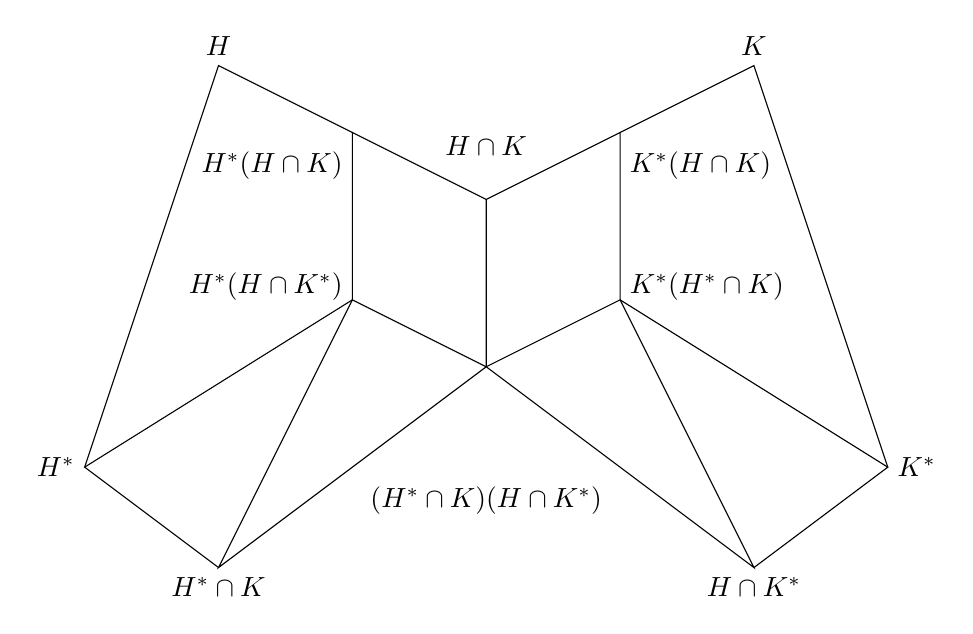
\begin{tikzpicture}[scale=1.7]

\draw  (0,0) -- (1,0.5) -- (2,-1.5) -- cycle;
\draw  (0,0) -- (0,1.25) -- (1,1.75) -- (1,0.5);
\draw (1,0.5) -- (3,-0.75) -- (2,-1.5) node [below] {$H \cap K^*$};
\draw (1,1.75) -- (2,2.25) node [above] {$K$} -- (3,-0.75) node [right] {$K^*$};
\node at (1, 0.6) [right] {$K^*(H^* \cap K)$};
\node at (1, 1.5) [right] {$K^*(H \cap K)$};


\draw  (0,0) -- (-1,0.5) -- (-2,-1.5) -- cycle;
\draw  (0,1.25) -- (-1,1.75) -- (-1,0.5);
\draw (-1,0.5) -- (-3,-0.75) -- (-2,-1.5) node [below] {$H^* \cap K$};
\draw (-1,1.75) -- (-2,2.25) node [above] {$H$} -- (-3,-0.75) node [left] {$H^*$};
\node at (-1, 0.6) [left] {$H^*(H \cap K^*)$};
\node at (-1, 1.5) [left] {$H^*(H \cap K)$};

\node at (0, -1) {$(H^* \cap K)(H \cap K^*)$};
\node at (0, 1.65) {$H \cap K$};

\end{tikzpicture}
\end{center}

\caption{The Zassenhaus Lemma}
\label{Butterfly}
\end{figure}
 
\item
\textbf{Schreier's Theorem.}\index{Schreier's Theorem}
Use the Zassenhaus Lemma to prove that two subnormal (normal) series 
of a group $G$ have isomorphic refinements.
 
 
\item
Use Schreier's Theorem to prove the  Jordan-H\"{o}lder Theorem.
 
\end{enumerate}
}
 
\subsection*{Programming Exercises}
 
{\small
Write a program that will compute all possible abelian
groups of order $n$.  What is the largest $n$ for which your
program will work?
}
 
 
 
\subsection*{References and Suggested Readings}  %%References checked and updated - TWJ 6/22/2010
 
{\small
Each of the following references contains a proof of the Fundamental
Theorem of Finitely Generated Abelian Groups.
\begin{itemize}
 
\item[\textbf{[1]}]   %%Reference updated 6/22/2010 - TWJ
Hungerford, T. W. 
\textit{Algebra}. Springer, New York, 1974. .
 
\item[\textbf{[2]}] %%Reference updated 6/22/2010 - TWJ
Lang, S. 
\textit{Algebra}. 3rd ed. Springer, New York, 2002.

 
\item[\textbf{[3]}] %%Reference updated 6/22/2010 - TWJ
Rotman, J. J. \textit{An Introduction to the Theory of
Groups}. 4th ed. Springer, New York, 1995.
 
 
\end{itemize}
}

\sagesection
 
 
 
 
   %Abelian and Solvable Groups
%%%%(c)
%%%%(c)  This file is a portion of the source for the textbook
%%%%(c)
%%%%(c)    Abstract Algebra: Theory and Applications
%%%%(c)    by Thomas W. Judson
%%%%(c)
%%%%(c)    Sage Material
%%%%(c)    Copyright 2011 by Robert A. Beezer
%%%%(c)
%%%%(c)  See the file COPYING.txt for copying conditions
%%%%(c)
%%%%(c)
\begin{sageverbatim}\end{sageverbatim}
%
\sageexercise{1}%
Construct the Higman-Sims graph with the command \verb?graphs.HigmanSimsGraph()?.  Then construct the automorphism group and determine the order of the one interesting normal subgroup of this group.  You can try plotting the graph, but the graphic is unlikely to be very informative.
\begin{sageverbatim}\end{sageverbatim}
%
\sageexercise{2}%
This exercise asks you to verify the class equation outside of the usual situation where the group action is conjugation.  Consider the example of the automorphism group of the path on 11 vertices.  First construct the list of orbits.  From each orbit, grab the first element of the orbit as a representative.  Compute the size of the orbit as the index of the stabilizer of the representative in the group via Theorem~\extref{orbit_theorem}{14.3}{theorem on orbit size as index}.  (Yes, you could just compute the size of the full orbit, but the idea of the exercise is to use more group-theoretic results.)  Then sum these orbit-sizes, which should equal the size of the whole vertex set since the orbits form a partition.
\begin{sageverbatim}\end{sageverbatim}
%
\sageexercise{3}%
Construct a graph, with at least two vertices and at least one edge, whose automorphism group is trivial.  You might start by drawing pictures before constructing the graph.  A command like the following will let you construct a graph from edges.  The graph below looks like a triangle or $3$-cycle.
%
\begin{sageexample}
sage: G = Graph([(1,2), (2,3), (3,1)])
sage: G.plot()            # not tested
\end{sageexample}
%
\begin{sageverbatim}\end{sageverbatim}
%
\sageexercise{4}%
For the following two pairs of groups, compute the list of conjugacy class representatives for each group in the pair.  For each part, compare and contrast the results for the two groups in the pair, with thoughtful and insightful comments.\\
(a) The full symmetric group on 5 symbols, $S_5$, and the alternating group on 5 symbols, $A_5$.\\
(b) The dihedral groups that are symmetries of a $7$-gon and an $8$-gon, $D_{7}$ and $D_{8}$.
\begin{sageverbatim}\end{sageverbatim}
%
\sageexercise{5}%
Use the command \verb?graphs.CubeGraph(4)? to build the four-dimensional cube graph, $Q_4$.  Using a plain \verb?.plot()? command (without a spring layout) should create a nice plot.  Construct the automorphism group of the graph and the translation between vertices of the graph and the symbols used in the automorphism group.  Then this group (and any of its subgroups) will provide a group action on the vertex set.\\
%
(a) Construct the orbits of this action, and comment.\\
(b) Construct a stabilizer of a single vertex (which is a subgroup of the full automorphism group) and then consider the action of \emph{this} group on the vertex set.  Construct the orbits of this new action, and comment carefully and fully on your observations, especially in terms of the vertices of the graph.
\begin{sageverbatim}\end{sageverbatim}
%
\sageexercise{6}%
Build the graph given by the commands below.  The result should be a symmetric-looking graph with an automorphism group of order 16.
%
% Graph is number 3.8 in Cvetkovic, Doob, Sachs
%
\begin{sageexample}
sage: G = graphs.CycleGraph(8)
sage: G.add_edges([(0,2),(1,3),(4,6),(5,7)])
sage: G.plot()                  # not tested
\end{sageexample}
%
Repeat parts (a) and (b) of the previous exercise, but realize that in part (b) there are now two different stabilizers to create, so build both and compare the differences in the stabilizers and their orbits.  Creating a second plot with \verb?G.plot(layout='planar')? might provide extra insight.\par
%
\emph{NOTE}: There was once a small bug with stabilizers being created as subgroups of symmetric groups on fewer symbols than the correct number.  This is fixed in Sage 4.8 and newer.  Note the correct output below, and you can check your installation by running these commands.  If you do not see the singleton \verb?[4]? in your output, you should definitely update your copy of Sage.
%
\begin{sageexample}
sage: G = SymmetricGroup(4)
sage: S = G.stabilizer(4)
sage: S.orbits()
[[1, 3, 2], [4]]
\end{sageexample}
%

  %Group Actions
%%%%(c)
%%%%(c)  This file is a portion of the source for the textbook
%%%%(c)
%%%%(c)    Abstract Algebra: Theory and Applications
%%%%(c)    by Thomas W. Judson
%%%%(c)
%%%%(c)    Sage Material
%%%%(c)    Copyright 2011 by Robert A. Beezer
%%%%(c)
%%%%(c)  See the file COPYING.txt for copying conditions
%%%%(c)
%%%%(c)
\sagesubsection{Sylow Subgroups}
%
The Sage permutation group method \verb?.sylow_subgroup(p)? will return a single Sylow $p$-subgroup.  If the prime is not a proper divisor of the group order it returns a subgroup of order $p^0$, in other words, a trivial subgroup.  So be careful about the primes you choose.  Sometimes, you may only want \emph{one} such Sylow subgroup, since any two Sylow $p$-subgroups are conjugate, and hence isomorphic (Theorem~\ref{sylow:Sylow_two_theorem}).  This also means we can create other Sylow $p$-subgroups by conjugating the one we have.  The permutation group method \verb?.conjugate(g)? will conjugate the group by \verb?g?.\par
%
With repeated conjugations of a single Sylow $p$-subgroup, we will likely create duplicate subgroups.  So we need to use a slightly complicated construction to form a list of just the unique subgroups in the list of conjugates.  The list comprehension will modify the list of unique subgroups, but also create some output we do not care about, so we assign the unwanted output to the variable \verb?junk?.\par
%
Lets investigate the Sylow subgroups of the dihedral group $D_{18}$.  As a group of order $36=2^2\cdot 3^2$, we know by the First Sylow Theorem that there is a Sylow $2$-subgroup of order $4$ and a Sylow $3$-subgroup of order $9$.  First for $p=2$, we obtain one Sylow $2$-subgroup, form all the conjugates, and form a list of non-duplicate subgroups.  (These commands take a while to execute, so be patient.)
%
\begin{sageexample}
sage: G = DihedralGroup(18)
sage: S2 = G.sylow_subgroup(2); S2
Subgroup of (Dihedral group of order 36 as a permutation group) 
generated by 
[(2,18)(3,17)(4,16)(5,15)(6,14)(7,13)(8,12)(9,11), 
(1,10)(2,11)(3,12)(4,13)(5,14)(6,15)(7,16)(8,17)(9,18)]
sage: allS2 = [S2.conjugate(g) for g in G]
sage: uniqS2 = []
sage: junk = [uniqS2.append(H) for H in allS2 if not H in uniqS2]
sage: uniqS2
[Permutation Group with generators 
[(2,18)(3,17)(4,16)(5,15)(6,14)(7,13)(8,12)(9,11), 
(1,10)(2,11)(3,12)(4,13)(5,14)(6,15)(7,16)(8,17)(9,18)], 
Permutation Group with generators 
[(1,3)(4,18)(5,17)(6,16)(7,15)(8,14)(9,13)(10,12), 
(1,10)(2,11)(3,12)(4,13)(5,14)(6,15)(7,16)(8,17)(9,18)], 
Permutation Group with generators 
[(1,5)(2,4)(6,18)(7,17)(8,16)(9,15)(10,14)(11,13), 
(1,10)(2,11)(3,12)(4,13)(5,14)(6,15)(7,16)(8,17)(9,18)], 
Permutation Group with generators 
[(1,7)(2,6)(3,5)(8,18)(9,17)(10,16)(11,15)(12,14), 
(1,10)(2,11)(3,12)(4,13)(5,14)(6,15)(7,16)(8,17)(9,18)], 
Permutation Group with generators 
[(1,9)(2,8)(3,7)(4,6)(10,18)(11,17)(12,16)(13,15), 
(1,10)(2,11)(3,12)(4,13)(5,14)(6,15)(7,16)(8,17)(9,18)], 
Permutation Group with generators 
[(1,10)(2,11)(3,12)(4,13)(5,14)(6,15)(7,16)(8,17)(9,18), 
(1,11)(2,10)(3,9)(4,8)(5,7)(12,18)(13,17)(14,16)], 
Permutation Group with generators 
[(1,10)(2,11)(3,12)(4,13)(5,14)(6,15)(7,16)(8,17)(9,18), 
(1,13)(2,12)(3,11)(4,10)(5,9)(6,8)(14,18)(15,17)], 
Permutation Group with generators 
[(1,10)(2,11)(3,12)(4,13)(5,14)(6,15)(7,16)(8,17)(9,18), 
(1,15)(2,14)(3,13)(4,12)(5,11)(6,10)(7,9)(16,18)], 
Permutation Group with generators 
[(1,10)(2,11)(3,12)(4,13)(5,14)(6,15)(7,16)(8,17)(9,18), 
(1,17)(2,16)(3,15)(4,14)(5,13)(6,12)(7,11)(8,10)]]
sage: len(uniqS2)
9
\end{sageexample}
%
The Third Sylow Theorem tells us that for $p=2$ we would expect $1, 3\text{ or }9$ Sylow $2$-subgroups, so our computational result of 9 subgroups is consistent with what the theory predicts.  Can you visualize each of these subgroups as symmetries of an $18$-gon?  Notice that we also have many subgroups of order $2$ inside of these subgroups of order $4$.
%
\begin{sageexample}
sage: G = DihedralGroup(18)
sage: S3 = G.sylow_subgroup(3); S3
Subgroup of (Dihedral group of order 36 as a permutation group) 
generated by 
[(1,7,13)(2,8,14)(3,9,15)(4,10,16)(5,11,17)(6,12,18), 
(1,15,11,7,3,17,13,9,5)(2,16,12,8,4,18,14,10,6)]
sage: allS3 = [S3.conjugate(g) for g in G]
sage: uniqS3 = []
sage: junk = [uniqS3.append(H) for H in allS3 if not H in uniqS3]
sage: uniqS3
[Permutation Group with generators 
[(1,7,13)(2,8,14)(3,9,15)(4,10,16)(5,11,17)(6,12,18), 
(1,15,11,7,3,17,13,9,5)(2,16,12,8,4,18,14,10,6)]]
sage: len(uniqS3)
1
\end{sageexample}
%
What does the Third Sylow Theorem predict?  Just $1$ or $4$ Sylow $3$-subgroups.  Having found just one subgroup computationally, we know that all of the conjugates of the lone Sylow $3$-subgroup are equal.  In other words, the Sylow $3$-subgroup is normal in $D_{18}$.  Let's check.
%
\begin{sageexample}
sage: S3.is_normal(G)
True
\end{sageexample}
%
At least one of the subgroups of order $3$ contained in this Sylow $3$-subgroup should be obvious by looking at the orders of the generators, and then you may even notice that the generators given could be reduced, and one is a power of the other.
%
\begin{sageexample}
sage: S3.is_cyclic()
True
\end{sageexample}
%
Remember that there are many other subgroups, of other orders.  For example, can you construct a subgroup of order $6=2\cdot 3$ in $D_{18}$?\par
%
\sagesubsection{Normalizers}
%
A new command that is relevant to this section is the construction of a normalizer.  The Sage command \verb?G.normalizer(H)? will return the subgroup of \verb?G? containing elements that normalize the subgroup \verb?H?.  We illustrate its use with the Sylow subgroups from above.
%
\begin{sageexample}
sage: G = DihedralGroup(18)
sage: S2 = G.sylow_subgroup(2)
sage: S3 = G.sylow_subgroup(3)
sage: N2 = G.normalizer(S2); N2
Subgroup of (Dihedral group of order 36 as a permutation group) 
generated by 
[(2,18)(3,17)(4,16)(5,15)(6,14)(7,13)(8,12)(9,11), 
(1,10)(2,11)(3,12)(4,13)(5,14)(6,15)(7,16)(8,17)(9,18)]
sage: N2 == S2
True
sage: N3 = G.normalizer(S3); N3
Subgroup of (Dihedral group of order 36 as a permutation group) 
generated by 
[(2,18)(3,17)(4,16)(5,15)(6,14)(7,13)(8,12)(9,11), 
(1,2)(3,18)(4,17)(5,16)(6,15)(7,14)(8,13)(9,12)(10,11), 
(1,7,13)(2,8,14)(3,9,15)(4,10,16)(5,11,17)(6,12,18), 
(1,15,11,7,3,17,13,9,5)(2,16,12,8,4,18,14,10,6)]
sage: N3 == G
True
\end{sageexample}
%
The normalizer of a subgroup always contains the whole subgroup, so the normalizer of \verb?S2? is as small as possible.  We already knew \verb?S3? is normal in \verb?G?, so it is no surprise that its normalizer is as big as possible --- every element of \verb?G? normalizes \verb?S3?.  Let's compute a normalizer in $D_{18}$ that is more ``interesting.''
%
\begin{sageexample}
sage: G = DihedralGroup(18)
sage: a = G("(1,7,13)(2,8,14)(3,9,15)(4,10,16)(5,11,17)(6,12,18)")
sage: b = G("(1,5)(2,4)(6,18)(7,17)(8,16)(9,15)(10,14)(11,13)")
sage: H = G.subgroup([a, b])
sage: H.order()
6
sage: N = G.normalizer(H)
sage: N
Subgroup of (Dihedral group of order 36 as a permutation group) 
generated by 
[(1,2)(3,18)(4,17)(5,16)(6,15)(7,14)(8,13)(9,12)(10,11), 
(1,5)(2,4)(6,18)(7,17)(8,16)(9,15)(10,14)(11,13), 
(1,13,7)(2,14,8)(3,15,9)(4,16,10)(5,17,11)(6,18,12)]
sage: N.order()
12
\end{sageexample}
%
So for this subgroup of order $6$, the normalizer is strictly bigger than the subgroup, but still strictly smaller than the whole group (and hence not normal in the dihedral group).  Trivially, a subgroup is normal in its normalizer:
%
\begin{sageexample}
sage: H.is_normal(G)
False
sage: H.is_normal(N)
True
\end{sageexample}
%
\sagesubsection{Finite Simple Groups}
%
We saw earlier Sage's permutation group method \verb?.is_simple()?.  Example~\ref{example:sylow:G_pn} tells us that a group of order $64$ is never simple.  The dicyclic group \verb?DiCyclicGroup(16)? is a non-abelian group of $64$, so we can test this method on this group.  It turns out this group has many normal subgroups --- the list will always contain the trivial subgroup and the group itself, so any number exceeding $2$ indicates a non-trivial normal subgroup.
%
\begin{sageexample}
sage: DC=DiCyclicGroup(16)
sage: DC.order()
64
sage: DC.is_simple()
False
sage: ns = DC.normal_subgroups()
sage: len(ns)
9
\end{sageexample}
%
Here is a rather interesting group, one of the 26 sporadic simple groups, known as the Higman-Sims group, $HS$.  The generators used below come from the representation on 100 points in GAP format, available off of \url{http://web.mat.bham.ac.uk/atlas/v2.0/spor/HS/}.  Generators of order 2 and order 5, roughly 44 million elements, but no normal subgroups.  Amazing.
%
\begin{sageexample}
sage: G = SymmetricGroup(100)
sage: a = G([(1,60),  (2,72),  (3,81),  (4,43),  (5,11),  (6,87),
...          (7,34),  (9,63),  (12,46), (13,28), (14,71), (15,42),
...          (16,97), (18,57), (19,52), (21,32), (23,47), (24,54),
...          (25,83), (26,78), (29,89), (30,39), (33,61), (35,56),
...          (37,67), (44,76), (45,88), (48,59), (49,86), (50,74),
...          (51,66), (53,99), (55,75), (62,73), (65,79), (68,82),
...          (77,92), (84,90), (85,98), (94,100)])
sage: b = G([(1,86,13,10,47),  (2,53,30,8,38),
...          (3,40,48,25,17),  (4,29,92,88,43),   (5,98,66,54, 65),
...          (6,27,51,73,24),  (7,83,16,20,28),   (9,23,89,95,61),
...          (11,42,46,91,32), (12,14, 81,55,68), (15,90,31,56,37),
...          (18,69,45,84,76), (19,59,79,35,93),  (21,22,64,39,100),
...          (26,58,96,85,77), (33,52,94,75,44),  (34,62,87,78,50),
...          (36,82,60,74,72), (41,80,70,49,67),  (57,63,71,99,97)])
sage: a.order()
2
sage: b.order()
5
sage: HS = G.subgroup([a, b])
sage: HS.order()
44352000
sage: HS.is_simple()
True
\end{sageexample}
%
We saw this group earlier in the exercises for Chapter~\ref{actions} on group actions, where it was the single non-trivial normal subgroup of the automorphism group of the Higman-Sims graph.
%
\sagesubsection{GAP Console and Interface}
%
This concludes our exclusive study of group theory, though we will be using groups some in the subsequent sections.  As we have remarked, much of Sage's computation with groups is performed by the open source program, ``Groups, Algorithms, and Programming,'' which is better know as simply GAP.  If after this course you outgrow Sage's support for groups, then learning GAP would be your next step as a group theorist. Every copy of Sage includes a copy of GAP and is easy to see which version of GAP is included:
%
\begin{sageexample}
sage: gap.version()
'4.7.5'
\end{sageexample}
%
You can interact with GAP in Sage in several ways. The most direct is by creating a permutation group via Sage's \verb?gap()? command.
%
\begin{sageexample}
sage: G = gap('Group( (1,2,3,4,5,6), (1,3,5) )')
sage: G
Group( [ (1,2,3,4,5,6), (1,3,5) ] )
\end{sageexample}
%
Now we can use most any GAP command with \verb?G?, via the convention that most GAP commands expect a group as the first argument, and we instead provide the group by using the \verb?G.? syntax.  If you consult the GAP documentation you will see that \verb?Center? is a GAP command that expects a group as its lone argument, and \verb?Centralizer? is a GAP command that expects two arguments --- a group and then a group element.
%
\begin{sageexample}
sage: G.Center()
Group( [ ( 1, 3, 5)( 2, 4, 6) ] )
sage: G.Centralizer('(1, 3, 5)')
Group( [ (1,3,5), (2,4,6), (1,3,5)(2,4,6) ] )
\end{sageexample}
%
In a worksheet you can set the first line of a compute cell to \verb?%gap? and the entire cell will be interpreted as if you were interacting directly with GAP.  This means you would now have to use GAP's syntax.  You can also use the drop-down box at the top of a worksheet, and select \verb?gap? as the system (rather than \verb?sage?) and the whole worksheet will be interpreted as GAP commands.  Here is one simple example, which you should be able to evaluate in your notebook.
%
\begin{sageverbatim}
%gap
G := Group( (1,2,3,4,5,6), (1,3,5) );
Centralizer(G, (1,3,5));
\end{sageverbatim}
%
Notice that
%
\begin{enumerate}
\item We do not need to wrap the individual permutations in as many quotation marks as we do in Sage.
\item Assignment is \verb?:=? not \verb?=?.  If you forget the colon, you will get an error message such as \texttt{Variable: 'G' must have a value}.
\item A line \emph{must} end with a semi-colon.  If you forget, several lines will be merged together.
\end{enumerate}
%
You can get help about GAP commands with a command such as the following, though you will soon see that GAP assumes you know a lot more algebra than Sage assumes you know.
%
\begin{sageverbatim}
print gap.help('SymmetricGroup', pager=False)
\end{sageverbatim}
%
In the command-line version of Sage, you can also use the GAP ``console.''  Again, you need to use GAP syntax, and you do not have many of the conveniences of the Sage notebook.  It is also good to know in advance that \verb?quit;? is how you can leave the GAP console and get back to Sage.  If you run Sage at the command-line, use the command \verb?gap_console()? to start GAP running.\par
%
It is a comfort to know that with Sage you get a complete copy of GAP, installed and all ready to run.  However, this is not a tutorial on GAP, so consult the documentation available at the main GAP website: \url{www.gap-system.org} to learn how to get the most out of it.
%
\begin{sageverbatim}
\end{sageverbatim}
%

    %Sylow Theorems
%%%%(c)
%%%%(c)  This file is a portion of the source for the textbook
%%%%(c)
%%%%(c)    Abstract Algebra: Theory and Applications
%%%%(c)    by Thomas W. Judson
%%%%(c)
%%%%(c)    Sage Material
%%%%(c)    Copyright 2011 by Robert A. Beezer
%%%%(c)
%%%%(c)  See the file COPYING.txt for copying conditions
%%%%(c)
%%%%(c)
Rings are very important in your study of abstract algebra, and similarly, they are very important in the design and use of Sage.  There is a lot of material in this chapter, and there are many corresponding commands in Sage.
%
\sagesubsection{Creating Rings}
%
Here is a list of various rings, domains and fields you can construct simply.\par
%
1. \verb?Integers()?, \verb?ZZ?: the integral domain of positive and negative integers, ${\mathbb Z}$.\par
%
2.  \verb?Integers(n)?: the integers mod $n$, ${\mathbb Z_n}$.  A field when $n$ is prime, but just a ring for composite $n$.\par
%
3.  \verb?QQ?: the field of rational numbers, ${\mathbb Q}$.\par
%
4.  \verb?RR?, \verb?CC?: the field of real numbers and the field of complex numbers, ${\mathbb R}$, ${\mathbb C}$.  It is impossible to create \emph{every} real number inside a computer, so technically these sets do not behave as fields, but only give a good imitiation of the real thing.  We say they are ``inexact'' rings to make this point.\par
%
5.  \verb?QuadraticField(n)?:  the field formed by combining the rationals with a solution to the polynomial equation $x^2-n=0$.  The notation in the text is ${\mathbb Q}[\sqrt{n}]$.  A functional equivalent can be made with the syntax \verb?QQ[sqrt(n)]?.  Note that \verb?n? can be negative.\par
%
6.  \verb?CyclotomicField(n)?: the field formed by combining the rationals with the solutions to the polynomial equation $x^n-1=0$.\par
%
7.  \verb?QQbar?: the field formed by combining the rationals with the solutions to \emph{every} polynomial equation with integer coefficients.  This is known as a the field of algebraic numbers, denoted as $\overline{{\mathbb Q}}$.\par
%
8.  \verb?FiniteField(p)?: For a prime $p$, the field of integers ${\mathbb Z_p}$.\par
%
If you print a description of some of the above rings, you will sometimes see a new symbol introduced.  Consider the following example:
%
\begin{sageexample}
sage: F = QuadraticField(7)
sage: F
Number Field in a with defining polynomial x^2 - 7
sage: root = F.gen(0)
sage: root^2
7
sage: root
a
sage: (2*root)^3
56*a
\end{sageexample}
%
Here \verb?Number Field? describes an object generally formed by combining the rationals with another number (here $\sqrt{7}$).  ``a'' is a new symbol which behaves as a root of the polynomial $x^2-7$.  We do not say which root, $\sqrt{7}$ or $-\sqrt{7}$, and as we understand the theory better we will see that this does not really matter.\par
%
We can obtain this root as a generator of the number field, and then manipulate it.  First squaring \verb?root? yields 7.  Notice that \verb?root? prints as \verb?a?.  Notice, too, that computations with \verb?root? behave as if it was \emph{either} root of $x^2-7$, and results print using \verb?a?.\par
%
This can get a bit confusing, inputing computations with \verb?root? and getting output in terms of \verb?a?.  Fortunately, there is a better way.  Consider the following example:
%
\begin{sageexample}
sage: F.<b> = QuadraticField(7)
sage: F
Number Field in b with defining polynomial x^2 - 7
sage: b^2
7
sage: (2*b)^3
56*b
\end{sageexample}
%
With the syntax \verb?F.<b>? we can create the field \verb?F? along with specifying a generator \verb?b? using a name of our choosing.  Then computations can use \verb?b? in both input and output as a root of $x^2-7$.\par
%
Here are three new rings that are best created using this new syntax.\par
%
1. \verb?F.<a> = FiniteField(p^n)?: We will later have a theorem that tells us that finite fields only exist with orders equal to to a power of a prime.  When the power is larger than 1, then we need a gnerator, here given as \verb?a?.\par
%
2. \verb?P.<x>=R[]?: the ring of all polynomials in the variable \verb?x?, with coefficients from the ring \verb?R?.  Notice that \verb?R? can be \emph{any} ring, so this is a very general construction that uses one ring to form another.  See an example below.\par
%
3. \verb?Q.<r,s,t> = QuaternionAlgebra(n, m)?: the rationals combined with indeterminates \verb?r?, \verb?s? and \verb?t? such that $r^2=n$, $s^2=m$ and $t = rs = -sr$.  This is a generalization of the quaternions described in this chapter, though over the rationals rather than the reals, so it is an exact ring.  Notice that this is one of the few noncommutative rings in Sage.  The ``usual'' quaternions would be constructed with \verb?Q.<I,J,K> = QuaternionAlgebra(-1, -1)?.  (Notice that using \verb?I? here is not a good choice, because it will then clobber the symbol \verb?I? used for complex numbers.)
\par
%
Syntax specifying names for generators can be used for many of the above rings as well, such as demonstrated above for quadratic fields and below for cyclotomic fields.
%
\begin{sageexample}
sage: C.<t> = CyclotomicField(8)
sage: C.random_element()  # random
-2/11*t^2 + t - 1
\end{sageexample}
%
\sagesubsection{Properties of Rings}
%
The examples below demonstrate how to query certain properties of rings.  If you are playing along, be sure to execute the first compute cell to define the various rings involved in the examples.
%
\begin{sageexample}
sage: Z7 = Integers(7)
sage: Z9 = Integers(9)
sage: Q = QuadraticField(-11)
sage: F.<a> = FiniteField(3^2)
sage: P.<x> = Z7[]
sage: S.<f,g,h> = QuaternionAlgebra(-7, 3)
\end{sageexample}
%
Exact versus inexact.
%
\begin{sageexample}
sage: QQ.is_exact()
True
sage: RR.is_exact()
False
\end{sageexample}
%
Finite versus infinite.
%
\begin{sageexample}
sage: Z7.is_finite()
True
sage: P.is_finite()
False
\end{sageexample}
%
Integral domain?
%
\begin{sageexample}
sage: Z7.is_integral_domain()
True
sage: Z9.is_integral_domain()
False
\end{sageexample}
%
Field?
%
\begin{sageexample}
sage: Z9.is_field()
False
sage: F.is_field()
True
sage: Q.is_field()
True
\end{sageexample}
%
Commutative?
%
\begin{sageexample}
sage: Q.is_commutative()
True
sage: S.is_commutative()
False
\end{sageexample}
%
Characteristic.
%
\begin{sageexample}
sage: Z7.characteristic()
7
sage: Z9.characteristic()
9
sage: Q.characteristic()
0
sage: F.characteristic()
3
sage: P.characteristic()
7
sage: S.characteristic()
0
\end{sageexample}
%
Additive and multiplicative identities \emph{print} like you would expect, but notice that while they may \emph{print} identically, they could be \emph{different} because of the ring they are in.
%
\begin{sageexample}
sage: b = Z9.zero(); b
0
sage: b.parent()
Ring of integers modulo 9
sage: c = Q.zero(); c
0
sage: c.parent()
Number Field in a with defining polynomial x^2 + 11
sage: b == c
False
sage: d = Z9.one(); d
1
sage: d.parent()
Ring of integers modulo 9
sage: e = Q.one(); e
1
sage: e.parent()
Number Field in a with defining polynomial x^2 + 11
sage: d == e
False
\end{sageexample}
%
There is some support for subrings.  For example, \verb?Q? and \verb?S? are extensions of the rationals, while \verb?F? is totally distinct from the rationals.
%
\begin{sageexample}
sage: QQ.is_subring(Q)
True
sage: QQ.is_subring(S)
True
sage: QQ.is_subring(F)
False
\end{sageexample}
%
Not every element of a ring may have a multiplicative inverse, in other words, not every element has to be a unit (unless the ring is a field).  It would now be good practice to check if an element is a unit before you try computing its inverse.
%
\begin{sageexample}
sage: three = Z9(3)
sage: three.is_unit()
False
sage: three*three
0
sage: four = Z9(4)
sage: four.is_unit()
True
sage: g = four^-1; g
7
sage: four*g
1
\end{sageexample}
%
\sagesubsection{Quotient Structure}
%
Ideals are the normal subgroups of rings and allow us to build ``quotients'' --- basically new rings defined on equivalence classes of elements of the original ring.  Sage support for ideals is variable.  When they can be created, there is not always a lot you can do with them.  But they work well in certain very important cases.
%
The integers, ${\mathbb Z}$, have ideals that are just multiples of a single integer.  We can create them with the \verb?.ideal()? method or just by wrting a scalar multiple of \verb?ZZ?.  And then the quotient is isomorphic to a well-understood ring.  (Notice that \verb?I? is a bad name for an ideal if we want to work with complex numbers later.)
%
\begin{sageexample}
sage: I1 = ZZ.ideal(4)
sage: I2 = 4*ZZ
sage: I3 = (-4)*ZZ
sage: I1 == I2
True
sage: I2 == I3
True
sage: Q = ZZ.quotient(I1); Q
Ring of integers modulo 4
sage: Q == Integers(4)
True
\end{sageexample}
%
We might normally be more careful about the last statement.  The quotient is a set of equivalence classes, each infinite, and certainly not a single integer.  But the quotient is \emph{isomorphic} to ${\mathbb Z}_4$, so Sage just makes this identification.\par
%
\begin{sageexample}
sage: Z7 = Integers(7)
sage: P.<y> = Z7[]
sage: M = P.ideal(y^2+4)
sage: Q = P.quotient(M)
sage: Q
Univariate Quotient Polynomial Ring in ybar over
Ring of integers modulo 7 with modulus y^2 + 4
sage: Q.random_element() # random
2*ybar + 6
sage: Q.order()
49
sage: Q.is_field()
True
\end{sageexample}
%
Notice that the construction of the quotient ring has created a new generator, converting \verb?y? ($y$) to \verb?ybar? ($\overline{y}$).  We can override this as before with the syntax demonstrated below.
%
\begin{sageexample}
sage: Q.<t> = P.quotient(M); Q
Univariate Quotient Polynomial Ring in t over
Ring of integers modulo 7 with modulus y^2 + 4
sage: Q.random_element() # random
4*t + 6
\end{sageexample}
%
So from a quotient of an infinite ring and an ideal (which is also a ring), we create a field, which is finite.  Understanding this construction will be an important theme in the next few chapters.  To see how remarkable it is, consider what happens with just one little change.
%
\begin{sageexample}
sage: Z7 = Integers(7)
sage: P.<y> = Z7[]
sage: M = P.ideal(y^2+3)
sage: Q.<t> = P.quotient(M)
sage: Q
Univariate Quotient Polynomial Ring in t over
Ring of integers modulo 7 with modulus y^2 + 3
sage: Q.random_element() #random
3*t + 1
sage: Q.order()
49
sage: Q.is_field()
False
\end{sageexample}
%
There are a few methods available which will give us properties of ideals.  In particular, we can check for prime and maximal ideals in rings of polynomials.  Examine the results above and below in the context of Theorem~\ref{theorem:maximalfield}.
%
\begin{sageexample}
sage: Z7 = Integers(7)
sage: P.<y> = Z7[]
sage: M = P.ideal(y^2+4)
sage: N = P.ideal(y^2+3)
sage: M.is_maximal()
True
sage: N.is_maximal()
False
\end{sageexample}
%
The fact that \verb?M? is a prime ideal is verification of Corollary~\ref{rings:max_ideal_corollary}.
%
\begin{sageexample}
sage: M.is_prime()
True
sage: N.is_prime()
False
\end{sageexample}
%
\sagesubsection{Ring Homomorphisms}
%
When Sage is presented with \verb?3 + 4/3?, how does it know that 3 is meant to be an integer? And then to add it to a rational, how does it know that we really want to view the computation as 3/1 + 4/3?  This is really easy for you and me, but devilishly hard for a program, and you can imagine it getting ever more complicated with the many possible rings in Sage, subrings, matrices, etc.  Part of the answer is that Sage uses ring homomorphisms to ``translate'' objects (numbers) between rings.\par
%
We will give an example below, but not pursue the topic much further.  For the curious, reading the Sage documentation and experimenting would be a good exercise.
%
\begin{sageexample}
sage: H = Hom(ZZ, QQ)
sage: phi = H([1])
sage: phi
Ring morphism:
  From: Integer Ring
  To:   Rational Field
  Defn: 1 |--> 1
sage: phi.parent()
Set of Homomorphisms from Integer Ring to Rational Field
sage: a = 3; a
3
sage: a.parent()
Integer Ring
sage: b = phi(3); b
3
sage: b.parent()
Rational Field
\end{sageexample}
%
So \verb?phi? is a homomorphism (``morphism'') that converts integers (the domain is \verb?ZZ?) into rationals (the codomain is \verb?QQ?), whose parent is a set of homomorphisms that Sage calls a ``homset.''  Even though \verb?a? and \verb?b? both print as \verb?3?, which is indistinguishable to our eyes, the parents of \verb?a? and \verb?b? are different.  Yet the numerical value of the two objects has not changed.
%




    %Introduction to Rings
%%%%(c)
%%%%(c)  This file is a portion of the source for the textbook
%%%%(c)
%%%%(c)    Abstract Algebra: Theory and Applications
%%%%(c)    by Thomas W. Judson
%%%%(c)
%%%%(c)    Sage Material
%%%%(c)    Copyright 2011 by Robert A. Beezer
%%%%(c)
%%%%(c)  See the file COPYING.txt for copying conditions
%%%%(c)
%%%%(c)
\begin{sageverbatim}\end{sageverbatim}
%
\sageexercise{1}%
Consider the polynomial $x^3-3x+4$.  Compute the most thorough factorization of this polynomial over each of the following fields:  (a) the finite field ${\mathbb Z}_5$, (b) a finite field with 125 elements, (c) the rationals, (d) the real numbers and (e) the complex numbers.  To do this, build the appropriate polynomial ring, and construct the polynomial as a member of this ring, and use the \verb?.factor()? method.
\begin{sageverbatim}\end{sageverbatim}
%
\sageexercise{2}%
``Conway polynomials'' are irreducible polynomials over ${\mathbb Z}_p$ that Sage (and other software) uses to build maximal ideals in polynomial rings, and thus quotient rings that are fields. Roughly speaking, they are ``canonical'' choices for each degree and each prime.  The command \verb?conway_polynomial(p, n)? will return a database entry that is an irreducible polynomial of degree $n$ over ${\mathbb Z}_p$.\par
%
Execute the command \verb?conway_polynomial(5, 4)? to obtain an allegedly irreducible polynomial of degree 4 over ${\mathbb Z}_5$:  $p = x^{4} + 4x^{2} + 4x + 2$.  First determine that p has no linear factors.  The only possibility left is that \verb?p? factors as two quadratic polynomials over ${\mathbb Z}_5$.  Use a list comprehension with \emph{three} \verb?for? statements to create \emph{every} possible quadratic polynomial over ${\mathbb Z}_5$.  Now use this list to create every possible product of two quadratic polynomials and check to see if \verb?p? is in this list.\par
%
More on Conway polynomials is available at
\url{http://www.math.rwth-aachen.de/~Frank.Luebeck/data/ConwayPol/index.html}
\begin{sageverbatim}\end{sageverbatim}
%
\sageexercise{3}%
Construct a finite field of order $729$ as a quotient of a polynomial ring by a principal ideal generated with a Conway polynomial.
\begin{sageverbatim}\end{sageverbatim}
%
\sageexercise{4}%
Define the polynomials $p = x^3 + 2x^2 + 2x + 4$ and $q = x^4 + 2x^2$ as polynomials with coefficients from the integers.  Compute \verb?gcd(p, q)? and verify that the result divides both \verb?p? and \verb?q? (just form a fraction in Sage and see that it simplifies cleanly, or use the \verb?.quo_rem()? method).\par
%
Proposition~\extref{poly:gcd_ther}{17.7}{existence of polynomial gcd} says there are polynomials $r(x)$ and $s(x)$ such that the greatest common divisor equals $r(x)p(x)+s(x)q(x)$, \emph{if the coefficients come from a field}.  Since here we have two polynomials over the integers, investigate the results returned by Sage for the extended gcd, \verb?xgcd(p, q)?.  In particular, show that the first result of the returned triple is a multiple of the gcd.  Then verify the ``linear combination'' property of the result.
\begin{sageverbatim}\end{sageverbatim}
%
\sageexercise{5}%
For a polynomial ring over a field, every ideal is principal.  Begin with the ring of polynomials over the rationals.  Experiment with constructing ideals using two generators and then see that Sage converts the ideal to a principal ideal with a single generator.  (You can get this generator with the ideal method \verb?.gen()?.)  Can you explain how this single generator is computed?
\begin{sageverbatim}\end{sageverbatim}
     %Polynomial Rings
%%%%(c)
%%%%(c)  This file is a portion of the source for the textbook
%%%%(c)
%%%%(c)    Abstract Algebra: Theory and Applications
%%%%(c)    Copyright 1997 by Thomas W. Judson
%%%%(c)
%%%%(c)  See the file COPYING.txt for copying conditions
%%%%(c)
%%%%(c)
\chap{Integral Domains}{domains}
 
One of the most important rings we study is the ring of integers.  It was our first example of an algebraic structure: the first polynomial
ring that we examined was ${\mathbb Z}[x]$.  We also know that the integers sit naturally inside the field of rational numbers, ${\mathbb
Q}$.  The ring of integers is the model for all integral domains.  In this chapter we will examine integral domains in general, answering
questions about the ideal structure of integral domains, polynomial rings over integral domains, and whether or not an integral domain can
be embedded in a field.
 

\section{Fields of Fractions}

Every field is also an integral domain; however, there are many integral domains that are not fields.  For example, the integers ${\mathbb Z}$ are an integral domain but not a field.  A question that naturally arises is how we might associate an integral domain with a field.  There is a natural way to construct the rationals ${\mathbb Q}$ from the integers: the rationals can be represented as formal quotients of two integers.  The rational numbers are certainly a field.  In fact, it can be shown that the rationals are the smallest field that contains the integers.  Given an integral domain $D$, our question now becomes how to construct a smallest field $F$ containing $D$.  We will do this in the same way as we constructed the rationals from the integers.  

An element $p/q \in {\mathbb Q}$ is the quotient of two integers $p$ and $q$; however, different pairs of integers can represent the same
rational number.  For instance, $1/2 = 2/4 = 3/6$. We know that 
\[
\frac{a}{b} = \frac{c}{d}
\]
if and only if $ad = bc$. A more formal way of considering this problem is to examine fractions in terms of equivalence relations.  We can think of elements in ${\mathbb Q}$ as ordered pairs in ${\mathbb Z} \times {\mathbb Z}$.  A quotient $p/q$ can be written as $(p, q)$.  For instance, $(3, 7)$ would represent the fraction $3/7$.  However, there are problems if we consider all possible pairs in ${\mathbb Z} \times {\mathbb Z}$.  There is no fraction $5/0$ corresponding to the pair $(5,0)$.  Also, the pairs $(3,6)$ and $(2,4)$ both represent the fraction $1/2$.  The first problem is easily solved if we require the second coordinate to be nonzero.  The second problem is solved by considering two pairs $(a, b)$ and $(c, d)$ to be equivalent if $ad = bc$.

If we use the approach of ordered pairs instead of fractions, then we can study integral domains in general.  Let $D$ be any integral domain and let 
\[
S = \{ (a, b) : a, b \in D \mbox{ and } b \neq 0 \}.
\]
Define a relation on $S$ by $(a, b) \sim (c, d)$ if $ad=bc$.

\begin{lemma}
The relation $\sim$ between elements of $S$ is an equivalence relation. 
\end{lemma}
 
\begin{proof}
Since $D$ is commutative, $ab = ba$; hence, $\sim$ is reflexive on $D$.
Now suppose that $(a,b) \sim (c,d)$. Then $ad=bc$ or $cb = da$.
Therefore, $(c,d) \sim (a, b)$ and the relation is symmetric. Finally,
to show that the relation is transitive, let $(a, b) \sim (c, d)$ and
$(c, d) \sim (e,f)$. In this case $ad=bc$ and $cf = de$. Multiplying
both sides of $ad=bc$ by $f$ yields
\[
a f d = a d f = b c f = b d e = bed.
\]
Since $D$ is an integral domain, we can deduce that $af = be$ or 
$(a,b ) \sim (e, f)$. \mbox{\hspace{1in}}
\end{proof}
 

\medskip
 

We will denote the set of equivalence classes on $S$ by $F_D$. We now
need to define the operations of addition and multiplication on
$F_D$.  Recall how fractions are added and multiplied in ${\mathbb
Q}$:
\begin{align*}
\frac{a}{b} + \frac{c}{d} & = \frac{ad + b c}{b d}; \\
\frac{a}{b} \cdot \frac{c}{d} & = \frac{ac}{b d}.
\end{align*}
It seems reasonable to define the operations of addition and
multiplication on $F_D$ in a similar manner.  If we denote the
equivalence class of $(a, b) \in S$ by $[a, b]$, then we are led to
define the operations of addition and multiplication on $F_D$ by
\[
[a, b] + [c, d] = [ad + b c,b d]
\]
and
\[
[a, b] \cdot [c, d] = [ac, b d],
\]
respectively.  The next lemma demonstrates that these operations are
independent of the choice of representatives from each equivalence
class.
 
 
\begin{lemma}
The operations of addition and multiplication on $F_D$ are well-defined.
\end{lemma}
 

\begin{proof}
We will prove that the operation of addition is well-defined.  The
proof that multiplication is well-defined is left as an exercise.
Let $[a_1, b_1] = [a_2, b_2]$ and $[c_1, d_1] =[ c_2, d_2]$.  We must
show that
\[
[a_1 d_1 + b_1 c_1,b_1 d_1] = [a_2 d_2 + b_2 c_2,b_2 d_2]
\]
or, equivalently, that
\[
(a_1 d_1 + b_1 c_1)( b_2 d_2) = (b_1 d_1) (a_2 d_2 + b_2 c_2).
\]
Since  $[a_1, b_1] = [a_2, b_2]$ and $[c_1, d_1] =[ c_2, d_2]$, we
know that $a_1 b_2 = b_1 a_2$ and $c_1 d_2 = d_1 c_2$.  Therefore,
\begin{align*}
(a_1 d_1 + b_1 c_1)( b_2 d_2) 
& = 
a_1 d_1 b_2 d_2 + b_1 c_1 b_2 d_2 \\
& =
a_1 b_2 d_1 d_2 + b_1 b_2 c_1 d_2 \\
& =
b_1 a_2 d_1 d_2 + b_1 b_2 d_1 c_2 \\
& = 
(b_1 d_1) (a_2 d_2 + b_2 c_2).
\end{align*}
\end{proof}
 

\begin{lemma}\label{domains:field_fractions_lemma}
The set of equivalence classes of $S$, $F_D$, under the equivalence
relation $\sim$, together with the operations of addition and 
multiplication defined~by
\begin{align*}
[a, b] + [c, d] & = [ad + b c, b d] \\
{[ a, b]} \cdot [c, d] & = [ac, b d],
\end{align*}
is a field.
\end{lemma}
 

\begin{proof}
The additive and multiplicative identities are $[0,1]$ and $[1,1]$, 
respectively. To show that $[0,1]$ is the additive identity, observe 
that
\[
[a, b] + [0, 1] =  [ a 1 + b 0, b 1] = [a,b].
\]
It is easy to show that $[1, 1]$ is the multiplicative identity. Let
$[a, b] \in F_D$ such that $a \neq 0$. Then $[b, a]$ is also in $F_D$
and $[a,b] \cdot [b, a] = [1,1]$; hence, $[b, a]$ is the
multiplicative inverse for $[a, b]$.  Similarly, $[-a,b]$ is the
additive inverse of $[a, b]$.  We leave as exercises the verification
of the associative and  commutative properties of multiplication in
$F_D$. We also leave it to the reader to show that $F_D$ is an abelian
group under addition.  
 
 
It remains to show that the distributive property holds in $F_D$;
however, 
\begin{align*}
[a, b] [e, f] + [c, d][ e, f ] 
& = 
[a e, b f ] + [c e, d f] \\
& =
[a e d f + b f c e, b d f^2 ] \\
& =
[a e d + b c e, b d f ] \\
& =
[a d e + b c e, b d f ] \\
& =
( [a, b]  + [c, d] ) [ e, f ] 
\end{align*}
and the lemma is proved.
\end{proof} 	


\medskip

The field $F_D$ in Lemma~\ref{domains:field_fractions_lemma} is called the \boldemph{field of
fractions}\index{Field!of fractions} or \boldemph{field of
quotients}\index{Field!of quotients} of the integral domain $D$.  
 

\begin{theorem}\label{domains:field_of_quotients_ther}
Let $D$ be an integral domain.  Then $D$ can be embedded in a field of
fractions $F_D$, where any element in $F_D$ can be expressed as the
quotient of two elements in $D$.  Furthermore, the field of fractions
$F_D$ is unique in the sense that if $E$ is any field containing $D$,
then there exists a map $\psi : F_D \rightarrow E$ giving an isomorphism
with a subfield of $E$ such that $\psi(a) = a$ for all elements $a \in
D$. 
\end{theorem}
 

\begin{proof}
We will first demonstrate that $D$ can be embedded in the field 
$F_D$.  Define a map $\phi : D \rightarrow F_D$ by $\phi(a) 
= [a, 1]$.  Then for $a$ and $b$ in $D$,
\[
\phi( a + b ) = [a+b, 1] = [a, 1] + [b, 1] = \phi(a ) + \phi(b)
\]
and
\[
\phi( a b ) = [a b, 1] = [a, 1]  [b, 1] = \phi(a ) \phi(b);
\]
hence, $\phi$ is a homomorphism.  To show that $\phi$ is one-to-one,
suppose that $\phi(a) = \phi( b)$.  Then $[a, 1] = [b, 1]$, or $a = a1
= 1b = b$. Finally, any element of $F_D$ can be expressed as the quotient
of two elements in $D$, since   
\[
\phi(a) [\phi(b)]^{-1} = [a, 1] [b, 1]^{-1} = [a, 1] \cdot [1, b]
= [a, b].
\]

%Typo corrected.  Suggested by Nathan Lander.
%TWJ 2/13/2012

 
Now let $E$ be a field containing $D$ and define a map $\psi :F_D
\rightarrow E$ by $\psi([a, b]) = a b^{-1}$.  To show that $\psi$ is
well-defined, let $[a_1, b_1] = [a_2, b_2]$. Then $a_1 b_2 = b_1 a_2$.
Therefore, $a_1 b_1^{-1} = a_2 b_2^{-1}$  and $\psi( [a_1, b_1]) =
\psi( [a_2, b_2])$.
 

If $[a, b ]$ and $[c, d]$ are in $F_D$, then
\begin{align*}
\psi( [a, b] + [c, d] ) 
& = \psi( [ad + b c, b d ] ) \\
& =  (ad +b c)(b d)^{-1} \\
& = a b^{-1} + c d^{-1} \\
& = \psi( [a, b] ) + \psi( [c, d] )
\end{align*}
and
\begin{align*}
\psi( [a, b] \cdot [c, d] ) & = \psi( [ac, b d ] )\\
 & =  (ac)(b d)^{-1}\\
& = a b^{-1}  c d^{-1}\\
 & = \psi( [a, b] )  \psi( [c, d] ).
\end{align*}
Therefore, $\psi$ is a homomorphism.
 

To complete the proof of the theorem, we need to show that $\psi$ is
one-to-one.  Suppose that $\psi( [a, b] ) = ab^{-1} = 0$. Then $a =
0b = 0$ and $[a, b] = [0, b]$.  Therefore, the kernel of $\psi$ is
the zero element $[ 0, b]$ in $F_D$, and $\psi$ is injective.
\mbox{\hspace{1in}}
\end{proof}
 

\begin{example}{rational_polys}
Since ${\mathbb Q}$ is a field, ${\mathbb Q}[x]$ is an integral domain. The
field of fractions of ${\mathbb Q}[x]$ is the set of all rational
expressions $p(x)/q(x)$, where $p(x)$ and $q(x)$ are polynomials over
the rationals and $q(x)$ is not the zero polynomial. We will denote 
this field by ${\mathbb Q}(x)$.\label{noteratpoly} 
\end{example}

 

We will leave the proofs of the following corollaries of Theorem~\ref{domains:field_of_quotients_ther}
as exercises. 
 

\begin{corollary}\label{domains:char_zero_rationals_corollary}
Let $F$ be a field of characteristic zero. Then $F$ contains a
subfield isomorphic to ${\mathbb Q}$.	       
\end{corollary}


\begin{corollary}\label{domains:char_p_Zp_corollary}
Let $F$ be a field of characteristic $p$. Then $F$ contains a
subfield isomorphic to ${\mathbb Z}_p$.	       
\end{corollary}
 


\section{Factorization in Integral Domains}

 
The building blocks of the integers are the prime numbers.  If $F$ is
a field, then irreducible polynomials in $F[x]$ play a role that is
very similar to that of the prime numbers in the ring of integers.
Given an arbitrary integral domain, we are led to the following
series of definitions. 
 

Let $R$ be a commutative ring with identity, and let $a$ and $b$ be
elements in $R$.  We say that $a$ \boldemph{divides} $b$, and write $a \mid
b$, if there exists an element $c \in R$ such that $b = ac$.  A \boldemph{
unit}\index{Unit} in $R$ is an element that has a multiplicative
inverse.  Two elements $a$ and $b$ in $R$ are said to be \boldemph{
associates}\index{Element!associate}\index{Associate elements} if
there exists a unit $u$ in $R$ such that $a = ub$.   
 

Let $D$ be an integral domain.  A nonzero element $p \in D$ that is
not a unit is said to be \boldemph{
irreducible}\index{Element!irreducible}\index{Irreducible element}
provided that whenever $p = ab$, either $a$ or $b$ is a unit.
Furthermore, $p$ is \boldemph{
prime}\index{Prime element}\index{Element!prime} if whenever $p \mid
ab$ either $p \mid a$ or $p \mid b$.


\begin{example}{Qxy}
It is important to notice that prime and irreducible elements do not
always coincide. Let $R$ be the subring (with identity) of ${\mathbb Q}[x, y]$ generated
by $x^2$, $y^2$, and $xy$.  Each of these elements is irreducible in
$R$; however, $xy$ is not prime, since $xy$ divides $x^2 y^2$ but does
not divide either $x^2$ or $y^2$.
\end{example}

%We are assuming that R is an integral domain and contains 1.  TWJ 8/9/2012

 
 
The Fundamental Theorem of Arithmetic states that every positive
integer $n > 1$ can be factored into a product of prime numbers $p_1
\cdots p_k$, where the $p_i$'s are not necessarily distinct. We also
know that such factorizations are unique up to the order of the
$p_i$'s. We can easily extend this result to the integers. The
question arises of whether or not such factorizations are possible in
other rings.  Generalizing this definition, we say an integral domain
$D$ is a \boldemph{unique factorization domain},\index{Unique
factorization domain (UFD)}\index{Domain!unique factorization} or \boldemph{
UFD}, if $D$ satisfies the following criteria.  
\begin{enumerate}
 
\item
Let $a \in D$ such that $a \neq 0$ and $a$ is not a unit.
Then $a$ can be written as the product of irreducible
elements in $D$.
 
\item %Definition corrected thanks to Pascal Honore - TWJ 9/10/2010
Let $a = p_1 \cdots p_r = q_1 \cdots q_s$, where the $p_i$'s and the
$q_i$'s are irreducible. Then $r=s$ and there is a $\pi \in S_r$ such
that $p_i$ and $q_{\pi(j)}$ are associates for \mbox{$j = 1, \ldots, r$}. 
 
\end{enumerate}


\begin{example}{Z_UFD}
The integers are a unique factorization domain by the Fundamental
Theorem of Arithmetic.
\end{example}
 


\begin{example}{not_a_UFD}
Not every integral domain is a unique factorization domain. The
subring ${\mathbb Z}[ \sqrt{3}\, i ] = \{ a + b \sqrt{3}\, i\}$ of the
complex numbers is an integral domain (Exercise~\ref{rings:gaussian_exercise}, Chapter~\ref{rings}). Let
$z = a + b \sqrt{3}\, i$ and define \mbox{$\nu : {\mathbb Z}[ \sqrt{3}\, i ]
\rightarrow {\mathbb N} \cup \{ 0 \}$} by $\nu( z) = |z|^2 = a^2 + 3 b^2$.
It is clear that $\nu(z) \geq 0$ with equality when $z = 0$. Also,
from our knowledge of complex numbers we know that $\nu(z w) = \nu(z)
\nu(w)$. It is easy to show that if $\nu(z) = 1$, then $z$ is a unit,
and that the only units of ${\mathbb Z}[ \sqrt{3}\, i ]$ are 1 and $-1$.   
 

We claim that 4 has two distinct factorizations into irreducible
elements: 
\[
4 = 2 \cdot 2 = (1 - \sqrt{3}\, i) (1 + \sqrt{3}\, i).
\]
We must show that each of these factors is an irreducible element in
${\mathbb Z}[ \sqrt{3}\, i ]$. If 2 is not irreducible, then $2 = z w$ for
elements $z, w$ in ${\mathbb Z}[ \sqrt{3}\, i ]$ where $\nu( z) = \nu(w) =
2$. However, there does not exist an element in $z$ in ${\mathbb
Z}[\sqrt{3}\, i ]$ such that $\nu(z) = 2$ because the equation $a^2 + 3
b^2 = 2$ has no integer solutions. Therefore, 2 must be irreducible. A
similar argument shows that both $1 - \sqrt{3}\, i$ and $1 + \sqrt{3}\, i$
are irreducible. Since 2 is not a unit multiple of either $1 - 
\sqrt{3}\, i$ or $1 + \sqrt{3}\, i$, 4 has at least two distinct
factorizations into irreducible elements.
\mbox{\hspace{1in}}
\end{example}
 

 
\subsection*{Principal Ideal Domains}
 

Let $R$ be a commutative ring with identity. Recall that a principal
ideal generated by $a \in R$ is an ideal of the form $\langle a
\rangle = \{ ra : r \in R \}$. An integral domain in which every ideal
is principal is called a \boldemph{principal ideal domain},\index{Principal
ideal domain (PID)}\index{Domain!principal ideal} or  \boldemph{PID}. 
 

\begin{lemma}\label{domains:PI_lemma}
Let $D$ be an integral domain and let $a, b \in D$.
Then  
\begin{enumerate}

\rm\item\it
$a \mid b \Leftrightarrow \langle b \rangle \subset \langle a
\rangle$. 

\rm\item\it
$a$ and $b$ are associates $\Leftrightarrow$ $\langle b \rangle =
\langle a \rangle$.

\rm\item\it
$a$ is a unit in $D$ $\Leftrightarrow$ $\langle a \rangle = D$.

\end{enumerate} 
\end{lemma}


\begin{proof}
(1)
Suppose that $a \mid b$. Then $b = ax$ for some $x \in D$. Hence, for
every $r$ in $D$, $br =(ax)r = a(xr)$ and $\langle b \rangle \subset
\langle a \rangle$. Conversely, suppose that $\langle b \rangle
\subset \langle a \rangle$. Then $b \in \langle a \rangle$.
Consequently, $b =a x$ for some $x \in D$.  Thus, $a \mid b$.
 

(2)
Since $a$ and $b$ are associates, there exists a unit $u$ such that 
$a = u b$.  Therefore, $b \mid a$ and $\langle a \rangle \subset 
\langle b \rangle$. Similarly, $\langle b \rangle \subset \langle a 
\rangle$. It follows that $\langle a \rangle = \langle b \rangle$.
Conversely, suppose that $\langle a \rangle = \langle b
\rangle$. By part (1), $a \mid b$ and $b \mid a$. Then $a = bx$ and $b
= ay$ for some $x, y \in D$. Therefore, $a = bx = ayx$. Since $D$ is
an integral domain, $x y =1$; that is, $x$ and $y$ are units and $a$
and $b$ are associates.   


(3)
An element $a \in D$ is a unit if and only if $a$ is an associate of
1. However, $a$ is an associate of 1 if and only if $\langle a \rangle
= \langle 1 \rangle = D$. 
\end{proof}


\begin{theorem}
Let $D$ be a PID and $\langle p \rangle$ be a nonzero ideal in $D$. 
Then $\langle p \rangle$ is a maximal ideal if and only if $p$ is
irreducible.
\end{theorem}


\begin{proof}
Suppose that $\langle p \rangle$ is a maximal ideal.  If some element
$a$ in $D$ divides $p$, then $\langle p \rangle \subset \langle a
\rangle$.  Since $\langle p \rangle$ is maximal, either $D = \langle
a \rangle$ or $\langle p \rangle = \langle a \rangle$.  Consequently,
either $a$ and $p$ are associates or $a$ is a unit.  Therefore, $p$
is irreducible.


Conversely, let $p$ be irreducible. If $\langle a \rangle$ is an
ideal in $D$ such that  $\langle p \rangle \subset \langle a \rangle
\subset D$, then $a \mid p$. Since $p$ is irreducible, either $a$ must
be a unit or $a$ and $p$ are associates. Therefore, either $D =
\langle a \rangle$ or $\langle p \rangle = \langle a \rangle$.  Thus,
$\langle p \rangle$ is a maximal ideal.
\end{proof}


\begin{corollary}\label{domains:irredPIDcorollary}
Let $D$ be a PID. If $p$ is irreducible, then $p$ is prime.
\end{corollary}


\begin{proof}
Let $p$ be irreducible and suppose that $p \mid ab$.  Then $\langle
ab \rangle \subset \langle p \rangle$. By Corollary~\ref{rings:max_ideal_corollary}, since
$\langle p \rangle$ is a maximal ideal, $\langle p \rangle$ must also
be a prime ideal. Thus, either $a \in \langle p \rangle$ or $b \in
\langle p \rangle$.  Hence, either $p \mid a $ or $p \mid b$. 
\end{proof}


\begin{lemma}\label{domains:ACC_lemma}
Let $D$ be a PID.  Let $I_1, I_2, \ldots$ be a set of ideals such that 
$I_1 \subset I_2 \subset \cdots$. Then there exists an integer $N$
such that $I_n = I_N$ for all $n \geq N$.
\end{lemma}

 

\begin{proof}
We claim that $I= \bigcup_{i=1}^\infty I_i$ is an ideal of $D$. Certainly
$I$ is not empty, since $I_1 \subset I$ and $0 \in I$. If $a, b \in I$,
then $a \in I_i$ and $b \in I_j$ for some $i$ and $j$ in ${\mathbb N}$.
Without loss of generality we can assume that $i \leq j$.  Hence, $a$
and $b$ are both in $I_j$ and so $a - b$ is also in $I_j$. Now let $r
\in D$ and $a \in I$. Again, we note that $a \in I_i$ for some
positive integer $i$.  Since $I_i$ is an ideal, $ra \in I_i$ and hence
must be in $I$. Therefore, we have shown that $I$ is an ideal in $D$.

%Typo corrected.  Suggested by C. Wall.  TWJ 2/16/2012


Since $D$ is a principal ideal domain, there exists an element 
$\overline{a} \in D$ that generates $I$. Since $\overline{a}$ is in 
$I_N$ for some $N \in {\mathbb N}$, we know that $I_N = I = \langle 
\overline{a} \rangle$. Consequently, $I_n = I_N$ for $n \geq N$.
\end{proof}		    
 

\medskip


Any commutative ring satisfying the condition in Lemma~\ref{domains:ACC_lemma} is said
to satisfy the \boldemph{ascending chain condition},\index{Ascending chain
condition} or \boldemph{ACC}.  Such rings are called \boldemph{
Noetherian rings},\index{Ring!Noetherian} after Emmy Noether.  


\begin{theorem}
Every PID is a UFD.
\end{theorem}
 

\begin{proof}
\emph{Existence of a factorization.}
Let $D$ be a PID and $a$ be a nonzero element in $D$ that is not a
unit. If $a$ is irreducible, then we are done. If not, then there
exists a factorization $a = a_1 b_1$, where neither $a_1$ nor $b_1$ is
a unit. Hence, $\langle a \rangle \subset \langle a_1 \rangle$. By
Lemma~\ref{domains:PI_lemma}, we know that $\langle a \rangle \neq \langle a_1 \rangle$;
otherwise, $a$ and $a_1$ would be associates and $b_1$ would be a unit,
which would contradict our assumption. Now suppose that $a_1 =  a_2
b_2$, where neither $a_2$ nor $b_2$ is a unit. By the same argument as
before, $\langle a_1 \rangle \subset \langle a_2 \rangle$.  We can
continue with this construction to obtain an ascending chain of ideals
\[
\langle a \rangle \subset \langle a_1 \rangle \subset \langle a_2
\rangle \subset \cdots.
\]
By Lemma~\ref{domains:ACC_lemma}, there exists a positive integer $N$ such that
$\langle a_n \rangle = \langle a_N \rangle$ for all $n \geq N$. 
Consequently, $a_N$ must be irreducible. We have now shown that $a$ is
the product of two elements, one of which must be irreducible.  

%Label repaired.  Suggested by R. Beezer.
%TWJ 12/19/2011


Now suppose that $a = c_1 p_1$, where $p_1$ is irreducible. If $c_1$
is not a unit, we can repeat the preceding argument to conclude that
$\langle a \rangle \subset \langle c_1 \rangle$. Either $c_1$ is
irreducible or $c_1 = c_2 p_2$, where $p_2$ is irreducible and $c_2$
is not a unit.  Continuing in this manner, we obtain another chain of
ideals
\[
\langle a \rangle \subset \langle c_1 \rangle \subset \langle c_2
\rangle \subset \cdots.	   
\]
This chain must satisfy the ascending chain condition; therefore, 
\[
a = p_1 p_2 \cdots p_r
\]
for irreducible elements $p_1, \ldots, p_r$.


\emph{Uniqueness of the factorization.}
To show uniqueness, let
\[
a= p_1 p_2 \cdots p_r = q_1 q_2 \cdots q_s,
\]
where each $p_i$ and each $q_i$ is irreducible.  Without loss of
generality, we can assume that $r < s$. Since $p_1$ divides $q_1 q_2
\cdots q_s$, by Corollary~\ref{domains:irredPIDcorollary} it must divide some $q_i$. By
rearranging the $q_i$'s, we can assume that $p_1 \mid q_1$; hence,
$q_1 = u_1 p_1$ for some unit $u_1$ in $D$. Therefore,
\[
a = p_1 p_2 \cdots p_r = u_1 p_1 q_2 \cdots q_s
\]
or 
\[
p_2 \cdots p_r = u_1 q_2 \cdots q_s.
\]
Continuing in this manner, we can arrange the $q_i$'s such that $p_2
= q_2, p_3 = q_3, \ldots, p_r = q_r$, to obtain
\[
u_1 u_2 \cdots u_r q_{r+1} \cdots q_s = 1.
\]
In this case $q_{r+1} \cdots q_s$ is a unit, which contradicts the
fact that $q_{r+1}, \ldots, q_s$ are irreducibles. Therefore, $r=s$
and the factorization of $a$ is unique.
\end{proof}
%Label repaired.  Suggested by R. Beezer.
%TWJ - 12/19/2011

\begin{corollary}
Let $F$ be a field.  Then $F[x]$ is a UFD.
\end{corollary}

\begin{example}{Zx_UFD}
Every PID is a UFD, but it is not the case that every UFD is a PID. In Corollary~\ref{domains:int_poly_UFD_corollary}, we will prove that ${\mathbb Z}[x]$ is a UFD.  However,
${\mathbb Z}[x]$ is not a PID.  Let $I = \{ 5 f(x) + x g(x) : f(x), g(x)  \in {\mathbb Z}[x] \}$.  We can easily show that $I$ is an ideal of 
${\mathbb Z}[x]$.  Suppose that $I = \langle p(x) \rangle$.  Since $5 \in I$,  $5 = f(x) p(x)$.  In this case $p(x) = p$ must be a constant.  Since $x  \in I$, $x = p g(x)$; consequently, $p = \pm 1$. However, it follows from this fact that $\langle p(x) \rangle = {\mathbb Z}[x]$. But this would 
mean that 3 is in $I$. Therefore, we can write $3 = 5 f(x) + x g(x)$ for  some $f(x)$ and $g(x)$ in ${\mathbb Z}[x]$.  Examining the constant term of  this polynomial, we see that $3 = 5 f(x)$, which is impossible. 
\end{example}


\subsection*{Euclidean Domains}

We have repeatedly used the division algorithm when proving results about either ${\mathbb Z}$ or $F[x]$, where $F$ is a field.  We
should now ask when a division algorithm is available for an integral domain. 

Let $D$ be an integral domain such that for each $a \in D$ there is  a nonnegative integer $\nu(a)$\label{notevaluation} satisfying the
following conditions. 
\begin{enumerate}
 
\item
If $a$ and $b$ are nonzero elements in $D$, then $\nu(a) \leq \nu(ab)$.  
 
\item
Let $a, b \in D$ and suppose that $b \neq 0$. Then there exist elements $q, r \in D$ such that $a = bq +r$ and either $r=0$ or
$\nu(r) < \nu(b)$. 
 
\end{enumerate}
Then $D$ is called a \boldemph{Euclidean domain}\index{Euclidean domain}\index{Domain!Euclidean} and $\nu$ is called a \boldemph{Euclidean valuation}\index{Euclidean valuation}.  


\begin{example}{abs_value}
Absolute value on ${\mathbb Z}$ is a Euclidean valuation.
\end{example}


\begin{example}{Fx_Euc_val}
Let $F$ be a field. Then the degree of a polynomial in $F[x]$ is a Euclidean valuation. 
\end{example}


\begin{example}{Gaussian_valuation}
Recall that the Gaussian integers in Example~\ref{example:rings:gaussian_ring} of Chapter~\ref{rings} are defined by
\[
{\mathbb Z}[i] = \{  a + b i : a, b \in {\mathbb Z} \}.
\]
We usually measure the size of a complex number $a + bi$ by its absolute value, $|a + bi| = \sqrt{ a^2 + b^2}$; however, $\sqrt{a^2 + b^2}$ may not be an integer. For our valuation we will let $\nu(a + bi) = a^2 + b^2$ to ensure that we have an integer.  

We claim that $\nu( a+ bi) = a^2 + b^2$ is a Euclidean valuation on ${\mathbb Z}[i]$. Let $z, w \in {\mathbb Z}[i]$.  Then $\nu( zw) = |zw|^2 =
|z|^2 |w|^2  = \nu(z) \nu(w)$.  Since $\nu(z) \geq 1$ for every nonzero $z \in {\mathbb Z}[i]$, $\nu( z) \leq \nu(z) \nu(w)$.

%correction to last sentence.  Suggested by R. Beezer.
%TWJ 2/6/2013

Next, we must show that for any $z= a+bi$ and $w = c+di$ in ${\mathbb Z}[i]$ with $w \neq 0$, there exist elements $q$ and $r$ in 
${\mathbb Z}[i]$  such that $z = qw + r$ with either $r=0$ or  $\nu(r) < \nu(w)$.  We can view $z$ and $w$ as elements in ${\mathbb
Q}(i) = \{ p + qi : p, q \in {\mathbb Q} \}$, the field of fractions of ${\mathbb Z}[i]$.  Observe that
\begin{align*}
z w^{-1} & = (a +b i) \frac{c -d i}{c^2 + d^2} \\
& =
\frac{ac + b d}{c^2 + d^2} + \frac{b c -ad}{c^2 + d^2}i \\
& =
\left( 
m_1 + \frac{n_1}{c^2 + d^2}
\right)
+ 
\left(
m_2 + \frac{n_2}{c^2 + d^2}
\right) i \\
& =
(m_1 + m_2 i) + \left( 
\frac{n_1}{c^2 + d^2}
+ 
\frac{n_2}{c^2 + d^2}i
\right) \\
& =
(m_1 + m_2 i) + (s + ti)
\end{align*}
in ${\mathbb Q}(i)$.  In the last steps we are writing the real and imaginary parts as an integer plus a proper fraction.  That is, we take
the closest integer $m_i$ such that the fractional part satisfies $|n_i / (a^2 + b^2)| \leq 1/2$.  For example, we write 
\begin{align*}
\frac{9}{8} & = 1 + \frac{1}{8} \\
\frac{15}{8} & = 2 - \frac{1}{8}.
\end{align*}
Thus, $s$ and $t$ are the ``fractional parts'' of $z w^{-1} = (m_1 + m_2 i) + (s + ti)$. We also know that $s^2 + t^2 \leq 1/4 + 1/4 =
1/2$.  Multiplying by $w$, we have
\[
z = z w^{-1} w = w (m_1 + m_2 i) + w (s + ti)  = q w + r,
\]
where $q = m_1 + m_2 i$ and $r =  w (s + ti)$.  Since $z$ and $qw$ are in ${\mathbb Z}[i]$, $r$ must be in ${\mathbb Z}[i]$.  Finally, we need to show that either $r = 0$ or $\nu(r) < \nu(w)$.  However,
\[
\nu(r) = \nu(w) \nu(s + ti) \leq \frac{1}{2} \nu(w) < \nu(w).
\]
\end{example}

\begin{theorem}
Every Euclidean domain is a principal ideal domain.
\end{theorem}
 
\begin{proof}
Let $D$ be a Euclidean domain and let $\nu$ be a Euclidean valuation
on $D$.  Suppose $I$ is a nontrivial ideal in $D$ and choose a nonzero
element $b \in I$ such that $\nu(b)$ is minimal for all $a \in I$. 
Since $D$ is a Euclidean domain, there exist elements $q$ and $r$ in
$D$ such that $a = bq +r$ and either $r=0$ or $\nu(r) < \nu(b)$. But
$r = a - bq$ is in $I$ since $I$ is an ideal; therefore, $r = 0$ by the
minimality of $b$. It follows that $a = bq$ and $I = \langle b
\rangle$. 
\end{proof}
 

\begin{corollary}
Every Euclidean domain is a unique factorization domain.
\end{corollary}


\subsection*{Factorization in $D[x]$}

One of the most important polynomial rings is ${\mathbb Z}[x]$.  One of the first questions that come to mind about ${\mathbb Z}[x]$ is whether or not it is a UFD.  We will prove a more general statement here.  Our first task is to obtain a more general version of Gauss's Lemma
(Theorem~\ref{poly:Gauss_lemma}).  

Let $D$ be a unique factorization domain and suppose that 
\[
p(x) = a_n x^n + \cdots + a_1 x + a_0
\]
in $D[x]$.  Then the \boldemph{content}\index{Polynomial!content of} of $p(x)$ is the greatest common divisor of $a_0, \ldots, a_n$.  We say
that $p(x)$ is \boldemph{primitive}\index{Primitive polynomial}\index{Polynomial!primitive} if $\gcd(a_0, \ldots, a_n ) = 1$.    

%Typo corrected.  Suggested by Nathan Lander.
%TWJ 2/13/2012

 
\begin{example}{poly_gcd}
In ${\mathbb Z}[x]$ the polynomial $p(x)= 5 x^4 - 3 x^3 + x -4$ is a primitive polynomial since the greatest common divisor of the
coefficients is 1; however, the polynomial $q(x) = 4 x^2 - 6 x + 8$ is not primitive since the content of $q(x)$ is 2.
\end{example}
 
\begin{theorem}[Gauss's Lemma]\label{domains:Gauss_lemma}\index{Gauss's Lemma}
Let $D$ be a UFD and let $f(x)$ and $g(x)$ be primitive polynomials in $D[x]$.  Then $f(x) g(x)$ is primitive.
\end{theorem}
 
\begin{proof}
Let $f(x) = \sum_{i=0}^{m} a_i x^i$ and $g(x) = \sum_{i=0}^{n} b_i x^i$.  Suppose that $p$ is a prime dividing the coefficients of $f(x)
g(x)$.  Let $r$ be the smallest integer such that $p \notdivide a_r$ and $s$ be the smallest integer such that $p \notdivide b_s$.  The
coefficient of $x^{r+s}$ in $f(x) g(x)$ is 
\[
c_{r+s} = a_0 b_{r+s} + a_1 b_{r+s-1} + \cdots + a_{r+s-1} b_1 +
a_{r+s} b_0. 
\]
Since $p$ divides $a_0, \ldots, a_{r-1}$ and $b_0, \ldots, b_{s-1}$, $p$ divides every term of $c_{r+s}$ except for the term $a_r b_s$.  However, since $p \mid c_{r+s}$, either $p$ divides $a_r$ or $p$ divides $b_s$. But this is impossible.
\end{proof}
 

\begin{lemma}
Let $D$ be a UFD, and let $p(x)$ and $q(x)$ be in $D[x]$. Then the
content of $p(x) q(x)$ is equal to the product of the contents of
$p(x)$ and~$q(x)$.
\end{lemma}

\begin{proof}
Let $p(x) = c p_1(x)$ and $q(x) = d q_1(x)$, where $c$ and $d$ are the
contents of $p(x)$ and $q(x)$, respectively.  Then $p_1(x)$ and
$q_1(x)$ are primitive. We can now write $p(x) q(x) = c d p_1(x)
q_1(x)$. Since $p_1(x) q_1(x)$ is primitive, the content of $p(x)
q(x)$ must be $cd$.
\end{proof}

\begin{lemma}\label{domains:UFD_factor_lemma}
Let $D$ be a UFD and $F$ its field of fractions. Suppose that $p(x)
\in D[x]$ and $p(x) = f(x) g(x)$, where $f(x)$ and $g(x)$ are in 
$F[x]$. Then $p(x) = f_1(x) g_1(x)$, where $f_1(x)$ and $g_1(x)$ are in
$D[x]$.  Furthermore, $\deg f(x) = \deg f_1(x)$ and $\deg g(x) = \deg
g_1(x)$. 
\end{lemma}

\begin{proof}
Let $a$ and $b$ be nonzero elements of $D$ such that $a f(x), b g(x)$
are in $D[x]$. We can find $a_1, b_2 \in D$ such that $a f(x) = a_1
f_1(x)$ and $b g(x) = b_1 g_1(x)$, where $f_1(x)$ and $g_1(x)$ are
primitive polynomials in $D[x]$. Therefore, $a b p(x) = (a_1 f_1(x))(
b_1 g_1(x))$.  Since $f_1(x)$ and $g_1(x)$ are primitive polynomials,
it must be the case that $ab \mid a_1 b_1$ by Gauss's Lemma. Thus there
exists a $c \in D$ such that $p(x) = c f_1(x) g_1(x)$. Clearly, $\deg
f(x) = \deg f_1(x)$ and $\deg g(x) = \deg g_1(x)$. 
\end{proof}

\medskip

The following corollaries are direct consequences of Lemma~\ref{domains:UFD_factor_lemma}. 

\begin{corollary}\label{domains:irred_poly_lemma}
Let $D$ be a UFD and $F$ its field of fractions.  A primitive
polynomial $p(x)$ in $D[x]$ is irreducible in $F[x]$ if and only if it
is irreducible in $D[x]$.
\end{corollary}

\begin{corollary}
Let $D$ be a UFD and $F$ its field of fractions.  If $p(x)$ is a monic
polynomial in $D[x]$ with $p(x) = f(x) g(x)$ in $F[x]$, then $p(x) =
f_1(x) g_1(x)$, where $f_1(x)$ and $g_1(x)$ are in $D[x]$. Furthermore,
$\deg f(x) = \deg f_1(x)$ and $\deg g(x) = \deg g_1(x)$.
\end{corollary}


\begin{theorem}
If $D$ is a UFD, then $D[x]$ is a UFD.
\end{theorem}
 
 
\begin{proof}
Let $p(x)$ be a nonzero polynomial in $D[x]$.  If $p(x)$ is a constant
polynomial, then it must have a unique factorization since $D$ is a
UFD. Now suppose that $p(x)$ is a polynomial of positive degree in
$D[x]$. Let $F$ be the field of fractions of $D$, and let $p(x) =
f_1(x) f_2(x) \cdots f_n(x)$ by a factorization of $p(x)$, where each
$f_i(x)$ is irreducible. Choose $a_i \in D$ such that $a_i f_i(x)$ is in
$D[x]$. There exist $b_1, \ldots, b_n \in D$ such that $a_i f_i(x) =
b_i g_i(x)$, where $g_i(x)$ is a primitive polynomial in $D[x]$. By 
Corollary \ref{domains:irred_poly_lemma}, each $g_i(x)$ is irreducible in $D[x]$. Consequently, 
we can write
\[
a_1 \cdots a_n p(x) = b_1 \cdots b_n g_1(x) \cdots g_n(x).
\]
Let $b = b_1 \cdots b_n$. Since $g_1(x) \cdots g_n(x)$ is primitive,
$a_1 \cdots a_n$ divides $b$. Therefore, $p(x) = a g_1(x) \cdots
g_n(x)$, where $a \in D$. Since $D$ is a UFD, we can factor $a$ as $u
c_1 \cdots c_k$, where $u$ is a unit and each of the $c_i$'s is
irreducible in $D$. 


We will now show the uniqueness of this factorization. Let
\[
p(x) = a_1 \cdots a_m f_1(x) \cdots f_n(x) = b_1 \cdots b_r g_1(x)
\cdots g_s(x)
\]
be two factorizations of $p(x)$, where all of the factors are
irreducible in $D[x]$.  By Corollary~\ref{domains:irred_poly_lemma}, each of the $f_i$'s and
$g_i$'s is irreducible in $F[x]$. The $a_i$'s and the $b_i$'s are
units in $F$. Since $F[x]$ is a PID, it is a UFD; therefore, $n=s$.
Now rearrange the $g_i(x)$'s so that $f_i(x)$ and $g_i(x)$ are
associates for $i = 1, \ldots, n$.  Then there exist $c_1, \ldots,
c_n$ and $d_1, \ldots, d_n$ in $D$ such that $(c_i / d_i) f_i(x) =
g_i(x)$ or $c_i f_i(x) = d_i g_i(x)$. The polynomials $f_i(x)$ and
$g_i(x)$ are primitive; hence, $c_i$ and $d_i$ are associates in $D$.
Thus, $a_1 \cdots a_m = u b_1 \cdots b_r$ in $D$, where $u$ is a unit
in $D$. Since $D$ is a unique factorization domain, $m =s$. Finally,
we can reorder the $b_i$'s so that $a_i$ and $b_i$ are associates for
each $i$. This completes the uniqueness part of the proof.   
\end{proof}


\medskip


The theorem that we have just proven has several obvious but important 
corollaries. 
 

\begin{corollary}
Let $F$ be a field. Then $F[x]$ is a UFD.
\end{corollary}


\begin{corollary}\label{domains:int_poly_UFD_corollary}
${\mathbb Z}[x]$ is a UFD.
\end{corollary}


\begin{corollary}
Let $D$ be a UFD. Then $D[x_1, \ldots, x_n]$ is a UFD. 
\end{corollary} 



\noindent \textbf{Remark.}
It is important to notice that every Euclidean domain is a PID and
every PID is a UFD. However, as demonstrated by our examples, the
converse of each of these statements fails.  There are principal
ideal domains that are not Euclidean domains, and there are unique
factorization domains that are not principal ideal domains (${\mathbb
Z}[x]$). 

\histhead

\noindent
Karl Friedrich Gauss\index{Gauss, Karl Friedrich}, born in Brunswick, Germany on April 30, 1777, is considered to be one of the greatest
mathematicians who ever lived.  Gauss was truly a child prodigy.  At the age of three he was able to detect errors in the books of his father's
business.  Gauss entered college at the age of 15.  Before the age of 20, Gauss was able to construct a regular 17-sided polygon with a ruler
and compass.  This was the first new construction of a regular $n$-sided polygon since the time of the ancient Greeks.  Gauss succeeded in showing that if $N= 2^{2^n}+1$ was prime, then it was possible to construct a regular $N$-sided polygon.  

Gauss obtained his Ph.D. in 1799 under the direction of Pfaff at the University of Helmstedt.  In his dissertation he gave the first complete proof of the Fundamental Theorem of Algebra, which states that every polynomial with real coefficients can be factored into linear factors over the complex numbers.  The acceptance of complex numbers was brought about by Gauss, who was the first person to use the notation of $i$ for $\sqrt{-1}$. 

Gauss then turned his attention toward number theory; in 1801, he published his famous book on number theory, \textit{Disquisitiones
Arithmeticae}.  Throughout his life Gauss was intrigued with this branch of mathematics.  He once wrote, ``Mathematics is the queen of the sciences, and the theory of numbers is the queen of mathematics.'' 

In 1807, Gauss was appointed director of the Observatory at the University of G\"{o}ttingen, a position he held until his death.  This position required him to study applications of mathematics to the sciences.  He succeeded in making contributions to fields such as astronomy, mechanics, optics, geodesy, and magnetism.  Along with Wilhelm Weber, he coinvented the first practical electric telegraph some years before a better version was invented by Samuel F. B. Morse. 

Gauss was clearly the most prominent mathematician in the world in the early nineteenth century. His status naturally made his discoveries
subject to intense scrutiny.  Gauss's  cold and distant personality many times led him to ignore the work of his contemporaries, making him many enemies.  He did not enjoy teaching very much, and young mathematicians who sought him out for encouragement were often
rebuffed.  Nevertheless, he had many outstanding students, including Eisenstein, Riemann, Kummer, Dirichlet, and Dedekind. Gauss also
offered a great deal of encouragement to Sophie Germain (1776--1831), who overcame the many obstacles facing women in her day to become a very prominent mathematician.  Gauss died at the age of 78 in G\"{o}ttingen on February 23, 1855.
\histbox

 
\markright{EXERCISES}
\section*{Exercises}
\exrule

{\small
\begin{enumerate}

% 2010/05/18 R Beezer, added squared-power on $a$ in valuation
\item
Let $z = a + b \sqrt{3}\, i$ be in ${\mathbb Z}[ \sqrt{3}\, i]$. If $a^2 +3 b^2 = 1$, show that $z$ must be a unit. Show that the only units of ${\mathbb Z}[ \sqrt{3}\, i ]$ are 1 and $-1$. 

\item
The Gaussian integers, ${\mathbb Z}[i]$, are a UFD.  Factor each of the following elements in ${\mathbb Z}[i]$ into a product of irreducibles.
\begin{multicols}{2}
\begin{enumerate}

\item 
5

\item 
$1 + 3i$

\item 
$6+8i$

\item 
2

\end{enumerate}
\end{multicols}

%*****************Theory---Fields of fractions****************
 
\item
Let $D$ be an integral domain. 
\begin{enumerate}
 
 \item
Prove that $F_D$ is an abelian group under the operation of addition.

 \item
Show that the operation of multiplication is well-defined in the field
of fractions, $F_D$.  
 
 \item
Verify the associative and commutative properties for multiplication
in $F_D$. 

\end{enumerate}


\item
Prove or disprove: Any subring of a field $F$ containing $1$ is an
integral domain.

\item
Prove or disprove: If $D$ is an integral domain, then every prime element in $D$ is also irreducible in $D$.

%Exercise suggested by R. Beezer. TWJ 5/15/2012


 
\item
Let $F$ be a field of characteristic zero. Prove that $F$ contains a
subfield isomorphic to ${\mathbb Q}$.
 
\item
Let $F$ be a field.
\begin{enumerate}

 \item
Prove that the field of fractions of $F[x]$, denoted by
$F(x)$\label{noteratfun},  is isomorphic to the set all rational
expressions $p(x) / q(x)$, where $q(x)$ is not the zero polynomial. 

 \item
Let $p(x_1, \ldots, x_n)$ and $q(x_1, \ldots, x_n)$ be polynomials in
$F[x_1, \ldots, x_n]$. Show that the set of all rational expressions
$p(x_1, \ldots, x_n) / q(x_1, \ldots, x_n)$ is isomorphic to the field
of fractions of $F[x_1, \ldots, x_n]$.  We denote the field of
fractions of $F[x_1, \ldots, x_n]$ by $F(x_1, \ldots,
x_n)$\label{noteratnvar}.    

\end{enumerate}


\item
Let $p$ be prime and denote the field of fractions of ${\mathbb Z}_p[x]$
by ${\mathbb Z}_p(x)$.  Prove that ${\mathbb Z}_p(x)$ is an infinite field
of characteristic $p$. 

 
\item
Prove that the field of fractions of the Gaussian integers, ${\mathbb
Z}[i]$, is 
\[
{\mathbb Q}(i) = \{ p + q i : p, q \in {\mathbb Q}  \}.
\]

 
\item
A field $F$ is called a \boldemph{prime
field}\index{Prime field}\index{Field!prime} if it has no proper
subfields. If $E$ is a subfield of $F$ and $E$ is a prime field, then  
$E$ is a \boldemph{prime
subfield}\index{Prime subfield}\index{Subfield!prime} of $F$. 
\begin{enumerate}
 
 \item
Prove that every field contains a unique prime subfield.
 
 \item
If $F$ is a field of characteristic 0, prove that the prime subfield
of $F$ is isomorphic to the field of rational numbers, ${\mathbb Q}$.
 
 \item
If $F$ is a field of characteristic $p$, prove that the prime subfield
of $F$ is isomorphic to  ${\mathbb Z}_p$. 
 
\end{enumerate}

 



%*****************Theory---Factorization**********************


 
 
 
\item
Let ${\mathbb Z}[ \sqrt{2}\, ] = \{ a + b \sqrt{2} : a, b \in {\mathbb Z} \}$. 
\begin{enumerate}

 \item
Prove that ${\mathbb Z}[ \sqrt{2}\, ]$ is an integral domain. 

 \item
Find all of the units in ${\mathbb Z}[\sqrt{2}\, ]$. 

 \item
Determine the field of fractions of ${\mathbb Z}[ \sqrt{2}\, ]$. 
 
 \item
Prove that  ${\mathbb Z}[ \sqrt{2} i ]$ is a Euclidean domain under the
Euclidean valuation $\nu( a + b \sqrt{2}\, i) = a^2 + 2b^2$. 
 
\end{enumerate}


\item
Let $D$ be a UFD. An element $d \in D$ is a \boldemph{greatest common
divisor of}\index{Greatest common divisor!of elements in a UFD} $a$
\boldemph{and} $b$ \boldemph{in} $D$ if $d \mid a$ and $d \mid b$ and $d$ is
divisible by any other element dividing both $a$ and $b$.  
\begin{enumerate}

 \item
If $D$ is a PID and $a$ and $b$ are both nonzero elements of $D$,
prove there exists a unique greatest common divisor of $a$ and $b$ up to associates. That is, if $d$ and $d'$ are both greatest common divisors of $a$ and $b$, then $d$ and $d'$ are associates.  We write $\gcd( a, b)$ for the greatest common divisor of $a$ and $b$. 

%Uniqueness statement qualified.  Suggested by R. Beezer. TWJ 5/15/2012

 \item
Let $D$ be a PID and $a$ and $b$ be nonzero elements of $D$. Prove
that there exist elements $s$ and $t$ in $D$ such that $\gcd(a, b) =
as + bt$.

\end{enumerate}


\item
Let $D$ be an integral domain. Define a relation on $D$ by $a \sim b$
if $a$ and $b$ are associates in $D$.  Prove that $\sim$ is an
equivalence relation on $D$.  


\item
Let $D$ be a Euclidean domain with Euclidean valuation $\nu$.  If $u$
is a unit in $D$, show that $\nu(u) = \nu(1)$.


\item
Let $D$ be a Euclidean domain with Euclidean valuation $\nu$.  If $a$
and $b$ are associates in $D$, prove that $\nu(a) = \nu(b)$.


\item
Show that ${\mathbb Z}[\sqrt{5}\, i]$ is not a unique factorization domain.



\item
Prove or disprove:  Every subdomain of a UFD is also a UFD.


\item
An ideal of a commutative ring $R$ is said to be \boldemph{finitely
generated}\index{Ring!finitely generated} if there exist elements
$a_1, \ldots, a_n$ in $R$ such that every element $r \in R$ can be
written as $a_1 r_1 + \cdots + a_n r_n$ for some $r_1, \ldots, r_n$ in
$R$.  Prove that $R$ satisfies the ascending chain condition if and
only if every ideal of $R$ is finitely generated.  


\item
Let $D$ be an integral domain with a descending chain of ideals $I_1
\supset I_2 \supset I_3 \supset \cdots$.  Suppose that there exists an $N$ such that
$I_k = I_N$ for all $k \geq N$. A ring satisfying this condition is
said to satisfy the \boldemph{descending chain condition},\index{Descending
chain condition} or \boldemph{DCC}. Rings satisfying the DCC are called
\boldemph{Artinian rings},\index{Ring!Artinian} after Emil
Artin\index{Artin, Emil}.  Show that if $D$ satisfies the descending chain condition, it must satisfy the ascending chain condition.
%Exercise corrected.  Suggested by K. Brooks.  TWJ - 5/15/2012
%Exercise corrected.  Suggested by R. Beezer.  TWJ - 8/9/2012


\item
Let $R$ be a commutative ring with identity. We define a \boldemph{
multiplicative subset}\index{Multiplicative subset} of $R$ to be a
subset $S$ such that $1 \in S$ and $ab \in S$ if $a, b \in S$. 
\begin{enumerate}

% 2010/05/18 R Beezer, too many s's, added two \ast to distinguish
 \item
Define a relation $\sim$ on $R \times S$ by $(a, s) \sim (a', s')$ if
there exists an $s^\ast \in S$ such that $s^\ast(s' a -s a') =0$. Show that
$\sim$ is an equivalence relation on $R \times S$.
 
 
 \item
Let $a/s$ denote the equivalence class of $(a,s) \in R \times S$ and
let $ S^{-1}R$ be the set of all equivalence classes with respect to
$\sim$.  Define  the operations of addition and multiplication on
$S^{-1} R$ by
\begin{align*}
\frac{a}{s} + \frac{b}{t} & = \frac{at + b s}{s t} \\
\frac{a}{s}  \frac{b}{t} & = \frac{a b}{s t},
\end{align*}
respectively. Prove that these operations are well-defined on $S^{-1}R$
and that $S^{-1}R$ is a ring with identity under these operations.
The ring $S^{-1}R$ is called the \boldemph{ring of
quotients}\index{Ring!of quotients} of $R$ with respect to $S$.


 
 \item
Show that the map $\psi : R \rightarrow S^{-1}R$ defined by $\psi(a)
= a/1$ is a ring homomorphism.
 
 \item
If $R$ has no zero divisors and $0 \notin S$, show that $\psi$ is
one-to-one.
 
 
\item
Prove that $P$ is a prime ideal of $R$ if and only if $S = R \setminus
P$ is a multiplicative subset of $R$. 
 
\item
If $P$ is a prime ideal of $R$ and $S = R \setminus P$, show that the
ring of quotients $S^{-1}R$ has a unique maximal ideal. Any ring
that has a unique maximal ideal is called a \boldemph{local
ring}\index{Ring!local}.  
 
 
\end{enumerate}



 
\end{enumerate}
}
 
 
 
\subsection*{References and Suggested Readings}
 
{\small
 
\begin{itemize}
 
\item[\textbf{[1]}] %Reference updated - TWJ 8/14/2010
Atiyah, M. F.  and MacDonald, I. G. \textit{Introduction to
Commutative Algebra}. Westview Press, Boulder, CO, 1994.
 


\item[\textbf{[2]}] %Reference updated - TWJ 8/14/2010
Zariski, O. and Samuel, P. \textit{Commutative Algebra}, vols. I
and II. Springer, New York, 1975, 1960. 
 
\end{itemize}
}
 
\sagesection
 

  %Integral Domains
%%%%(c)
%%%%(c)  This file is a portion of the source for the textbook
%%%%(c)
%%%%(c)    Abstract Algebra: Theory and Applications
%%%%(c)    by Thomas W. Judson
%%%%(c)
%%%%(c)    Sage Material
%%%%(c)    Copyright 2011 by Robert A. Beezer
%%%%(c)
%%%%(c)  See the file COPYING.txt for copying conditions
%%%%(c)
%%%%(c)
\begin{sageverbatim}\end{sageverbatim}
%
\sageexercise{1}%
Use  \verb?R = Posets.RandomPoset(30,0.05)? to construct a random poset.  Use \verb?R.plot()? to get an idea of what you have built.\\
%
(a) Illustrate the use of the poset methods\\
\verb?.is_lequal()?\\
\verb?.is_less_than()?\\
\verb?.is_gequal()?\\
\verb?.is_greater_than()?\\
to determine if two elements are related or incomparable.\\
%
(b) Use \verb?.minimal_elements()? and \verb?,maximal_elements()? to find the smallest and largest elements of your poset.\\
%
(c) Use \verb?LatticePoset(R)? to see if the poset \verb?R? is a lattice by attempting to convert it into a lattice.\\
%
(d) Find a linear extension of your poset.  Confirm that consecutive elements of the output are comparable in the orginal lattice, and that they compare properly.
\begin{sageverbatim}\end{sageverbatim}
%
\sageexercise{2}%
Construct the poset on the positive divisors of $72=2^3\cdot 3^2$ with divisiblity as the relation, and then convert to a lattice.\\
%
(a) Determine the one and zero element using \verb?.top()? and \verb?.bottom()?.\\
%
(b) Determine all the pairs of elements of the lattice that are complements of each other \emph{without} using the \verb?.complement()? method, but rather just use the \verb?.meet()? and \verb?.join()? methods.  Extra credit if you can output each pair just once.\\
%
(c) Determine if the lattice is distributive using just the \verb?.meet()? and \verb?.join()? methods, and not the \verb?.is_distributive()? method.
\begin{sageverbatim}\end{sageverbatim}
%
\sageexercise{3}%
Construct several diamond lattices with \verb?Posets.DiamondPoset(n)? by varying the value of \verb?n?.  Give answers, with justifications, to these questions for \emph{general} $n$, based on observations obtained from experiments with Sage.\\
%
(a) Which elements have complements and which do not, and why?\\
%
(b) Read the documentation of the \verb?.antichains()? method to learn what an antichain is.  How many antichains are there?\\
%
(c) Is the lattice distributive?
\begin{sageverbatim}\end{sageverbatim}
%
\sageexercise{4}%
Use \verb?Posets.BooleanLattice(4)? to construct an instance of the prototypical Boolean algebra on 16 elements (i.e.\ all subsets of a $4$-set).\par
%
Then use \verb?Posets.IntegerCompositions(5)? to construct the poset whose 16 elements are the compositions of the integer $5$.  We have seen above that the integer composition lattice is distributive and complemented, making it a Boolean algebra.  And by Theorem~\extref{boolean:classification_boolean_algebra}{19.12}{classify boolean algebras} we can conclude that these two Boolean algebras are isomorphic.\par
%
Plot each to see the similarity, as follows.  Use the method \verb?.hasse_diagram()? on each poset to get back a directed graph and ask for their plots.  Then use the graph method \verb?.is_isomorphic()? to see that the two Hasse diagrams really are the same.
\begin{sageverbatim}\end{sageverbatim}
%
\sageexercise{5}%
(Advanced) For the previous question, construct an explicit isomorphism between the two Boolean algebras.  This would be a bijective function (constructed with the \verb?def? command) that converts compositions into sets (or if, you choose, sets into compositions) and which respects the meet and join operations.  You can test and illustrate your function by its interaction with specific elements evaluated in the meet and join operations, as described in the definition of an isomorphism of Boolean algebras.
  %Lattices and Boolean Algebras
%%%%(c)
%%%%(c)  This file is a portion of the source for the textbook
%%%%(c)
%%%%(c)    Abstract Algebra: Theory and Applications
%%%%(c)    Copyright 1997 by Thomas W. Judson
%%%%(c)
%%%%(c)  See the file COPYING.txt for copying conditions
%%%%(c)
%%%%(c)
\chap{Vector Spaces}{vect}


 
In a physical system a quantity can often be described with a single
number. For example, we need to know only a single number to describe
temperature, mass, or volume.  However, for some quantities, such as
location, we need several numbers. To give the location of a point in
space, we need $x$, $y$, and $z$ coordinates. Temperature
distribution over a solid object requires four numbers: three to
identify each point within the object and a fourth to describe the
temperature at that point.  Often $n$-tuples of numbers, or vectors,
also have certain algebraic properties, such as addition or scalar 
multiplication.  


In this chapter we will examine mathematical structures called vector
spaces. As with groups and rings, it is desirable to give a simple
list of axioms that must be satisfied to make a set of vectors a
structure worth studying.  
 
 
 
\section{Definitions and Examples}
 

A \boldemph{vector space}\index{Vector space!definition of} $V$ over a
field $F$ is an abelian group with a \boldemph{scalar
product}\index{Scalar product} $\alpha \cdot v$ or $\alpha v$ defined
for all $\alpha \in F$ and all $v \in V$ satisfying the following
axioms.  
\begin{itemize}

\item 
$\alpha(\beta v) =(\alpha \beta)v$;

\item 
$(\alpha + \beta)v =\alpha v + \beta v$;

\item 
$\alpha(u + v) = \alpha u + \alpha v$;

\item 
$1v=v$;

\end{itemize}
where $\alpha, \beta \in F$ and $u, v \in V$.
 

The elements of $V$ are called \boldemph{vectors}; the elements of $F$
are called \boldemph{scalars}.  It is important to notice that in most
cases two vectors cannot be multiplied.  In general, it is only
possible to multiply a vector with a scalar. To differentiate between
the scalar zero and the vector zero, we will write them as 0 and
${\mathbf 0}$, respectively.  


Let us examine several examples of vector spaces. Some of them will be
quite familiar; others will seem less so.
 
 
\begin{example}{vector_space_Rn}
The $n$-tuples of real numbers, denoted by ${\mathbb R}^n$, form a vector
space over ${\mathbb R}$. Given vectors $u = (u_1, \ldots, u_n)$ and $v =
(v_1, \ldots, v_n)$ in ${\mathbb R}^n$ and $\alpha$ in ${\mathbb R}$, we can
define vector addition by
\[
u + v = (u_1, \ldots, u_n) + (v_1, \ldots, v_n)
=
(u_1 + v_1, \ldots, u_n + v_n)
\]
and scalar multiplication by 
\[
\alpha u = \alpha(u_1, \ldots, u_n)= (\alpha u_1, \ldots, \alpha u_n).
\]
\end{example}
 
 
 
\begin{example}{vector_space_Fx}
If $F$ is a field, then $F[x]$ is a vector space over $F$. The vectors
in $F[x]$ are simply polynomials.  Vector addition is just polynomial
addition. If $\alpha \in F$ and $p(x) \in F[x]$, then scalar
multiplication is defined by $\alpha p(x)$.
\end{example}
 
 
\begin{example}{vector_space_cont}
The set of all continuous real-valued functions on a closed interval
$[a,b]$ is a vector space over ${\mathbb R}$.  If $f(x)$ and $g(x)$ are
continuous on $[a, b]$, then $(f+g)(x)$ is defined to be $f(x) +
g(x)$.  Scalar multiplication is defined by
$(\alpha f)(x) = \alpha f(x)$ for $\alpha \in 
{\mathbb R}$. For example, if $f(x) = \sin x$ and $g(x)= x^2$, then 
$(2f+5g)(x) =2 \sin x + 5 x^2$. 
\end{example}
 

 
\begin{example}{vector_space_sqrt2}
Let $V = {\mathbb Q}(\sqrt{2}\, ) = \{ a + b \sqrt{2} : a, b \in 
{\mathbb Q } \}$. Then $V$ is a
vector space over ${\mathbb Q}$. If $u = a + b \sqrt{2}$ and $v = c + d
\sqrt{2}$, then $u + v = (a + c) + (b + d ) \sqrt{2}$ is again in $V$.
Also, for $\alpha \in {\mathbb Q}$, $\alpha v$ is in $V$.  We will leave
it as an exercise to verify that all of the vector space axioms hold
for $V$. 
\end{example}

 
\begin{proposition}
Let $V$ be a vector space over $F$. Then each of the following
statements is true. 
\begin{enumerate}

\rm \item \it 
$0v ={\mathbf 0}$ for all $v \in V$.

\rm \item \it 
$\alpha {\mathbf 0} = {\mathbf 0}$ for all $\alpha \in F$.


\rm \item \it 
If $\alpha v = {\mathbf 0}$, then either $\alpha = 0$ or $v = {\mathbf
0}$.  

\rm \item \it
$(-1) v = -v$ for all $v \in V$.

\rm \item \it 
$-(\alpha v) = (-\alpha)v = \alpha(-v)$ for all $\alpha \in F$ and all
$v \in V$. 

\end{enumerate}
\end{proposition}


\begin{proof}
To prove (1), observe that 
\[
0 v = (0 + 0)v = 0v + 0v;
\]
consequently, ${\mathbf 0} + 0 v = 0v + 0v$. Since $V$ is an abelian
group, ${\mathbf 0} = 0v$. 


The proof of (2) is almost identical to the proof of (1). For (3), we
are done if $\alpha = 0$.  Suppose that $\alpha \neq 0$. Multiplying
both sides of $\alpha v = {\mathbf 0}$ by $1/ \alpha$, we have $v =
{\mathbf 0}$.


To show (4), observe that
\[
v + (-1)v = 1v + (-1)v = (1-1)v = 0v = {\mathbf 0},
\]
and so $-v = (-1)v$. We will leave the proof of (5) as an exercise.
\end{proof}
 
 
 
\section{Subspaces}


Just as groups have subgroups and rings have subrings, vector spaces
also have substructures. Let $V$ be a vector space over a field $F$,
and $W$ a subset of $V$. Then $W$ is a \boldemph{subspace}\index{Vector
space!subspace of} of $V$ if it is closed under vector addition and
scalar multiplication; that is, if $u, v \in W$ and $\alpha
\in F$, it will always be the case that $u+v$ and $\alpha v$ are also
in $W$.   
 

 
\begin{example}{subspace_W}
Let $W$ be the subspace of ${\mathbb R}^3$ defined by $W = \{ (x_1, 2 x_1
+ x_2, x_1 - x_2) : x_1, x_2 \in {\mathbb R} \}$. We claim that $W$ is a 
subspace of ${\mathbb R}^3$.  Since 
\begin{align*}
\alpha (x_1, 2 x_1 + x_2, x_1 - x_2) 
& =  (\alpha x_1, \alpha(2 x_1 + x_2), \alpha( x_1 - x_2)) \\
& =  (\alpha x_1, 2(\alpha x_1) + \alpha x_2, \alpha x_1 -\alpha x_2),
\end{align*}
$W$ is closed under scalar multiplication. To show that $W$ is closed
under vector addition, let $u = (x_1, 2 x_1 + x_2, x_1 - x_2)$ and $v
= (y_1, 2 y_1 + y_2, y_1 - y_2)$ be vectors in $W$. Then
\[
u + v = 
(x_1 + y_1, 2( x_1 + y_1) +( x_2 + y_2), (x_1 + y_1) - (x_2+ y_2)).
\]
\end{example}
 
 
 
\begin{example}{subspace_poly}
Let $W$ be the subset of polynomials of $F[x]$ with no odd-power
terms. If $p(x)$ and $q(x)$ have no odd-power terms, then neither will 
$p(x) + q(x)$.  Also, $\alpha p(x) \in W$ for $\alpha \in F$ and $p(x)
\in W$.
\end{example}
  

% 2010/05/18 R Beezer, "vector field" to "vector space"
Let $V$ be any vector space over a field $F$ and suppose that $v_1,
v_2, \ldots, v_n$ are vectors in $V$ and $\alpha_1, \alpha_2, \ldots,
\alpha_n$ are scalars in $F$. Any vector $w$ in $V$ of the form
\[
w = \sum_{i=1}^n \alpha_i v_i = \alpha_1 v_1 + \alpha_2 v_2 + \cdots + \alpha_n v_n
\]
is called a \boldemph{linear combination}\index{Linear combination} of the
vectors $v_1, v_2, \ldots, v_n$. The \boldemph{spanning
set}\index{Spanning set} of vectors $v_1, v_2, \ldots, v_n$ is the
set of vectors obtained from all possible linear combinations of
$v_1, v_2, \ldots, v_n$. If $W$ is the spanning set of $v_1, v_2,
\ldots, v_n$, then we often say that $W$ is \boldemph{spanned} by $v_1,
v_2, \ldots, v_n$. 
 
 
\begin{proposition}
Let $S= \{v_1, v_2, \ldots, v_n \}$ be vectors in a vector space $V$.
Then the span of $S$ is a subspace of $V$. 
\end{proposition}


\begin{proof}
Let $u$ and $v$ be in $S$. We can write both of these vectors as 
linear combinations of the $v_i$'s:
\begin{align*}
u & =  \alpha_1 v_1 + \alpha_2 v_2 + \cdots + \alpha_n v_n \\
v & =  \beta_1 v_1 + \beta_2 v_2 + \cdots + \beta_n v_n.
\end{align*}
Then
\[
u+ v =( \alpha_1 + \beta_1) v_1 + (\alpha_2+ \beta_2) v_2 + \cdots +
(\alpha_n + \beta_n) v_n 
\]
is a linear combination of the $v_i$'s. For $\alpha \in F$,
\[
\alpha u = (\alpha \alpha_1) v_1 + ( \alpha \alpha_2) v_2 + \cdots +
(\alpha \alpha_n ) v_n 
\]
is in the span of $S$.
\end{proof}


 
\section{Linear Independence}
 

Let $S = \{v_1, v_2, \ldots, v_n\}$ be a set of vectors in a vector
space $V$. If there exist scalars $\alpha_1, \alpha_2 \ldots \alpha_n
\in F$ such that not all of the $\alpha_i$'s are zero and 
\[
\alpha_1 v_1 + \alpha_2 v_2 + \cdots + \alpha_n v_n = {\mathbf 0 },
\]
then $S$ is said to be \boldemph{linearly
dependent}\index{Linear dependence}. If the set $S$ is not linearly
dependent, then it is said to be \boldemph{linearly
independent}\index{Linear independence}. More specifically, $S$ is a
linearly independent set if
\[ 
\alpha_1 v_1 + \alpha_2 v_2 + \cdots + \alpha_n v_n = {\mathbf 0 }
\]
implies that
\[
\alpha_1 = \alpha_2 = \cdots = \alpha_n = 0
\]
for any set of scalars $\{ \alpha_1, \alpha_2 \ldots \alpha_n \}$.


 
\begin{proposition}
Let $\{ v_1, v_2, \ldots, v_n \}$ be a set of linearly independent
vectors in a vector space. Suppose that 
\[
v = \alpha_1 v_1 + \alpha_2 v_2 + \cdots + \alpha_n v_n
= \beta_1 v_1 + \beta_2 v_2 + \cdots + \beta_n v_n.
\]
Then $\alpha_1 = \beta_1, \alpha_2 = \beta_2, \ldots, \alpha_n =
\beta_n$. 
\end{proposition}

\begin{proof}
If 
\[
v = \alpha_1 v_1 + \alpha_2 v_2 + \cdots + \alpha_n v_n
= \beta_1 v_1 + \beta_2 v_2 + \cdots + \beta_n v_n,
\]
then
\[
(\alpha_1 - \beta_1) v_1 + (\alpha_2 - \beta_2) v_2 + \cdots +
(\alpha_n - \beta_n) v_n = {\mathbf 0}.
\]
Since $v_1, \ldots, v_n$ are linearly independent, $\alpha_i - \beta_i
=0$ for $i = 1, \ldots, n$.
\end{proof}
 

\medskip


The definition of linear dependence makes more sense if we consider
the following proposition.

 
\begin{proposition}
A set $\{ v_1, v_2, \dots, v_n \}$ of vectors in a vector space $V$ is
linearly dependent if and only if one of the $v_i$'s is a linear
combination of the rest. 
\end{proposition}


\begin{proof}
Suppose that $\{ v_1, v_2, \dots, v_n \}$ is a set of linearly dependent
vectors.  Then there exist scalars $\alpha_1, \ldots, \alpha_n$
such that
\[
\alpha_1 v_1 + \alpha_2 v_2 + \cdots + \alpha_n v_n = {\mathbf 0 },
\]
with at least one of the $\alpha_i$'s not equal to zero.  Suppose that
$\alpha_k \neq 0$. Then 
\[
v_k = - \frac{\alpha_1}{\alpha_k} v_1 
- \cdots 
- \frac{\alpha_{k-1}}{\alpha_k}	v_{k-1}
- \frac{\alpha_{k+1}}{\alpha_k}	v_{k+1}
- \cdots 
- \frac{\alpha_n}{\alpha_k} v_n.
\]


Conversely, suppose that 
\[
v_k = \beta_1 v_1 
+ \cdots 
+ \beta_{k-1} v_{k-1}
+ \beta_{k+1} v_{k+1}
+ \cdots 
+ \beta_n v_n.
\]
Then
\[
\beta_1 v_1 
+ \cdots 
+ \beta_{k-1} v_{k-1}
- v_k
+ \beta_{k+1} v_{k+1}
+ \cdots 
+ \beta_n v_n = {\mathbf 0}.
\]
\end{proof}

\medskip


The following proposition is a consequence of the fact that any system
of homogeneous linear equations with more unknowns than equations will
have a nontrivial solution.  We leave the details of the proof for the
end-of-chapter exercises. 
 

\begin{proposition}\label{vect:linearlyindependent}
Suppose that a vector space $V$ is spanned by $n$ vectors. If $m > n$,
then any set of $m$ vectors in $V$ must be linearly dependent. 
\end{proposition}
 
  
A set $\{ e_1, e_2, \ldots, e_n \}$ of vectors in a vector space $V$
is called a \boldemph{basis}\index{Vector space!basis of} for $V$ if $\{
e_1, e_2, \ldots, e_n \}$ is a linearly independent set that spans
$V$.

 
 
\begin{example}{basis_R3}
The vectors $e_1 = (1, 0, 0)$, $e_2 = (0, 1, 0)$, and $e_3 =(0, 0, 1)$
form a basis for ${\mathbb R}^3$.  The set certainly spans ${\mathbb R}^3$,
since any arbitrary vector $(x_1, x_2, x_3)$ in ${\mathbb R}^3$ can be
written as $x_1 e_1 + x_2 e_2 + x_3 e_3$. Also, none of the vectors
$e_1, e_2, e_3$ can be written as a linear combination of the other
two; hence, they are linearly independent.  The vectors $e_1, e_2,
e_3$ are not the only basis of ${\mathbb R}^3$:  the set $\{ (3, 2, 1),
(3, 2, 0), (1, 1, 1) \}$ is also a basis for ${\mathbb R}^3$. 
\end{example}

 
 
\begin{example}{basis_sqrt2}
Let ${\mathbb Q}( \sqrt{2}\, ) = \{ a + b \sqrt{2} : a, b \in {\mathbb Q} \}$.
The sets $\{1, \sqrt{2}\,  \}$ and $\{1+\sqrt{2}, 1- \sqrt{2}\,  \}$ are
both bases of ${\mathbb Q}( \sqrt{2}\, )$.  
\end{example}





From the last two examples it should be clear that a given vector
space has several bases. In fact, there are an infinite number of
bases for both of these examples. \emph{In general, there is no unique 
basis for a vector space}.  However, every basis of ${\mathbb R}^3$ consists
of exactly three vectors, and every  basis of ${\mathbb Q}(\sqrt{2}\, )$ 
consists of exactly two vectors. This is a consequence of the next 
proposition.


\begin{proposition}
Let $\{ e_1, e_2, \ldots, e_m \}$ and $\{ f_1, f_2, \ldots, f_n \}$ be
two bases for a vector space $V$. Then $m=n$. 
\end{proposition}


\begin{proof}
Since $\{ e_1, e_2, \ldots, e_m \}$ is a basis, it is a linearly
independent set.  By  Proposition~\ref{vect:linearlyindependent}, $n \leq m$. Similarly, $\{
f_1, f_2, \ldots, f_n \}$ is a linearly independent set, and the last
proposition implies that $m \leq n$.  Consequently, $m =n$.
\mbox{\hspace{1in}}
\end{proof}
%Label repaired.  Suggested by R. Beezer.
%TWJ - 12/19/2011
 

\medskip
 

If $\{ e_1, e_2, \ldots, e_n \}$ is a basis for a vector space $V$,
then we say that the \boldemph{dimension}\index{Vector space!dimension of}
of $V$ is $n$ and we write $\dim V =n$\label{vectdim}. 
We will leave the proof of the following theorem as an exercise.


\begin{theorem}
Let $V$ be a vector space of dimension $n$.
\begin{enumerate}

\rm \item \it
If $S = \{v_1, \ldots, v_n \}$ is a set of linearly independent
vectors for $V$, then $S$ is a basis for $V$. 

\rm \item \it
If $S = \{v_1, \ldots, v_n \}$ spans $V$, then $S$ is a basis for $V$. 

\rm \item \it
If $S = \{v_1, \ldots, v_k \}$ is a set of linearly independent
vectors for $V$ with $k < n$, then there exist vectors $v_{k+1},
\ldots, v_n$ such that  
\[
\{v_1, \ldots, v_k, v_{k+1}, \ldots, v_n \}
\]
is a basis for $V$. 

\end{enumerate}
\end{theorem}


 
\markright{EXERCISES}
\section*{Exercises}
\exrule

 
{\small
\begin{enumerate}

  
\item
If $F$ is a field, show that $F[x]$ is a vector space over $F$, where
the vectors in $F[x]$ are polynomials.  Vector addition is polynomial
addition, and scalar multiplication is defined by $\alpha p(x)$ for
$\alpha \in F$.  

\item
Prove that ${\mathbb Q }( \sqrt{2}\, )$ is a vector space.


\item
Let ${\mathbb Q }( \sqrt{2}, \sqrt{3}\, )$ be the field generated by
elements of the form $a + b \sqrt{2}  + c \sqrt{3}$, where $a, b, c$
are in ${\mathbb Q}$. Prove that ${\mathbb Q }( \sqrt{2}, \sqrt{3}\, )$ is a
vector space of dimension 4 over ${\mathbb Q}$.  Find a basis for 
${\mathbb Q }( \sqrt{2}, \sqrt{3}\, )$.


\item 
Prove that the complex numbers are a vector space of dimension 2
over ${\mathbb R}$. 


\item
Prove that the set $P_n$ of all polynomials of degree less than $n$
form a subspace of the vector space $F[x]$. Find a basis for $P_n$ and
compute the dimension of~$P_n$. 


\item
Let $F$ be a field and denote the set of $n$-tuples of $F$ by $F^n$.
Given vectors $u = (u_1, \ldots, u_n)$ and $v = (v_1, \ldots, v_n)$ in
$F^n$ and $\alpha$ in $F$, define vector addition by
\[
u + v = (u_1, \ldots, u_n) + (v_1, \ldots, v_n)
=
(u_1 + v_1, \ldots, u_n + v_n)
\]
and scalar multiplication by 
\[
\alpha u = \alpha(u_1, \ldots, u_n)= (\alpha u_1, \ldots, \alpha u_n).
\]
Prove that $F^n$ is a vector space of dimension $n$ under these
operations. 


\item
Which of the following sets are subspaces of ${\mathbb R}^3$? If the set
is indeed a subspace, find a basis for the subspace and compute its
dimension.
\begin{enumerate}

  \item
$\{ (x_1, x_2, x_3) : 3 x_1 - 2 x_2 + x_3 = 0 \}$

  \item
$\{ (x_1, x_2, x_3) : 3 x_1 + 4 x_3 = 0, 2 x_1 - x_2 + x_3 = 0 \}$

  \item
$\{ (x_1, x_2, x_3) : x_1 - 2 x_2 + 2 x_3 = 2 \}$

  \item
$\{ (x_1, x_2, x_3) : 3 x_1 - 2 x_2^2 = 0 \}$

\end{enumerate}


\item
Show that the set of all possible solutions $(x, y, z) \in {\mathbb R}^3$
of the equations
\begin{align*}
Ax + B y + C z & =  0 \\
D x + E y + C z & =  0
\end{align*}
form a subspace of ${\mathbb R}^3$.


\item
Let $W$ be the subset of continuous functions on $[0, 1]$ such that
$f(0) = 0$.  Prove that $W$ is a subspace of $C[0, 1]$.


%*******************THEORY***********************


\item
Let $V$ be a vector space over $F$. Prove that $-(\alpha v) =
(-\alpha)v = \alpha(-v)$ for all $\alpha \in F$ and all $v \in V$. 


\item
Let $V$ be a vector space of dimension $n$. Prove each of the
following statements. 
\begin{enumerate}

 \item
If $S = \{v_1, \ldots, v_n \}$ is a set of linearly independent
vectors for $V$, then $S$ is a basis for $V$. 

 \item
If $S = \{v_1, \ldots, v_n \}$ spans $V$, then $S$ is a basis for $V$.

 \item 
If $S = \{v_1, \ldots, v_k \}$ is a set of linearly independent
vectors for $V$ with $k < n$, then there exist vectors $v_{k+1},
\ldots, v_n$ such that 
\[
\{v_1, \ldots, v_k, v_{k+1}, \ldots, v_n \}
\]
is a basis for $V$. 

\end{enumerate}


\item
Prove that any set of vectors containing ${\mathbf 0}$ is linearly
dependent. 


\item
Let $V$ be a vector space. Show that $\{ {\mathbf 0} \}$ is a subspace
of $V$ of dimension zero.


\item
If a vector space $V$ is spanned by $n$ vectors, show that any set of
$m$ vectors in $V$ must be linearly dependent for $m > n$.  


\item \label{vect:linear_transformation}
\textbf{Linear Transformations.}
Let $V$ and $W$ be vector spaces over a field $F$, of dimensions $m$
and $n$, respectively. If $T: V \rightarrow W$ is a map satisfying
\begin{align*}
T( u+ v ) & =  T(u ) + T(v) \\
T( \alpha v ) & =  \alpha T(v)
\end{align*}
for all $\alpha \in F$ and all $u, v \in V$, then $T$ is called a
\boldemph{linear transformation}\index{Linear transformation!definition
of} from $V$ into $W$. 
\begin{enumerate}

   \item
Prove that the \boldemph{kernel}\index{Kernel!of a linear
transformation}\index{Linear transformation!kernel of} of $T$, 
$\ker(T) = \{ v \in V : T(v) = 
{\mathbf 0} \}$, is a subspace of $V$. The kernel of $T$ is sometimes
called the \boldemph{null space}\index{Null space!of a linear
transformation}\index{Linear transformation!null space of} of $T$. 

   \item
Prove that the \boldemph{range}\index{Linear transformation!range of} or
\boldemph{range space} of $T$, $R(V) = \{ w \in W : T(v) = w \text{ for
some } v \in V \}$, is a subspace of $W$.

   \item
Show that $T : V \rightarrow W$ is injective if and only if 
$\ker(T) = \{ \mathbf 0 \}$.

   \item
Let $\{ v_1, \ldots, v_k \}$ be a basis for the null space of $T$. We
can extend this basis to be a basis $\{ v_1, \ldots, v_k, v_{k+1},
\ldots, v_m\}$ of $V$. Why?  Prove that $\{ T(v_{k+1}), \ldots, T(v_m)
\}$ is a basis for the range of $T$. Conclude that the range of $T$
has dimension $m-k$.

   \item
Let $\dim V = \dim W$.  Show that a linear transformation $T : V
\rightarrow W$ is injective if and only if it is surjective.

\end{enumerate}


\item
Let $V$ and $W$ be finite dimensional vector spaces of dimension $n$
over a field $F$. Suppose that  $T: V \rightarrow W$ is a vector space
isomorphism.  If $\{ v_1, \ldots, v_n \}$ is a basis of $V$, show that
$\{ T(v_1), \ldots, T(v_n) \}$ is a basis of $W$. Conclude that any
vector space over a field $F$ of dimension $n$ is isomorphic to $F^n$. 


\item
\textbf{Direct Sums.} 
Let $U$ and $V$ be subspaces of a vector space $W$. The sum of $U$ and
$V$, denoted $U + V$, is defined to be the set of all vectors of the
form $u + v$, where $u \in U$ and $v \in V$. 
\begin{enumerate}

   \item
Prove that $U + V$ and $U \cap V$ are subspaces of $W$.

   \item
If $U + V = W$ and $U \cap V = {\mathbf 0}$, then $W$ is said to be the
\boldemph{direct sum}\index{Direct sum of vector spaces}\index{Vector
space!direct sum of} of $U$ and $V$ and we write $W = U \oplus
V$\label{notedirectsum}.
Show that every element $w \in W$ can be written uniquely as $w = u +
v$, where $u \in U$ and $v \in V$.

   \item
Let $U$ be a subspace of dimension $k$ of a vector space $W$ of
dimension $n$. Prove that there exists a subspace $V$ of dimension
$n-k$ such that $W = U \oplus V$.  Is the subspace $V$ unique?

   \item
If $U$ and $V$ are arbitrary subspaces of a vector space $W$, show
that 
\[
\dim( U + V) = \dim U + \dim V - \dim( U \cap V).
\]

\end{enumerate}


\item
\textbf{Dual Spaces.} 
Let $V$ and $W$ be finite dimensional vector spaces over a field~$F$. 
\begin{enumerate}

   \item
Show that the set of all linear transformations from $V$ into $W$,
denoted by $\Hom(V, W)$\label{noteHom}, 
is a vector space over $F$, where we
define vector addition as follows:
\begin{align*}
(S + T)(v) &=  S(v) +T(v) \\
(\alpha S)(v) & =  \alpha S(v),
\end{align*}
where $S, T \in \Hom(V, W)$, $\alpha \in F$, and $v \in V$.
 
   \item
Let $V$ be an $F$-vector space.  Define the \boldemph{dual
space}\index{Vector space!dual of} of $V$ 
to be $V^\ast = \Hom(V, F)$\label{notedual}. Elements in the dual space of $V$ are
called \boldemph{linear functionals}\index{Linear functionals}.  Let $v_1,
\ldots, v_n$ be an ordered basis for $V$. If $v = \alpha_1 v_1 +
\cdots + \alpha_n v_n$ is any vector in $V$, define a linear
functional  $\phi_i : V \rightarrow F$ by $\phi_i (v) = \alpha_i$.
Show that the $\phi_i$'s form a basis for $V^\ast$.  This basis is
called the \boldemph{dual basis} of $v_1, \ldots, v_n$ (or simply the dual
basis if the context makes the meaning clear).  
 

   \item
Consider the basis $\{ (3, 1), (2, -2) \}$ for ${\mathbb R}^2$. What is
the dual basis for $({\mathbb R}^2)^\ast$? 
 
   \item
Let $V$ be a vector space of dimension $n$ over a field $F$ and let
$V^{\ast \ast}$ be the dual space $V^\ast$.  Show that each element $v
\in V$ gives rise to an element $\lambda_v$ in $V^{\ast \ast}$ and
that the map $v \mapsto \lambda_v$ is an isomorphism of $V$ with
$V^{\ast \ast}$. 

\end{enumerate}
 

\end{enumerate}
}


 
\subsection*{References and Suggested Readings}  %References updated - TWJ 8/19/2010
 

{\small
\begin{itemize}

\item[\textbf{[1]}] %Reference added - TWJ 8/19/2010
Beezer, R. \textit{A First Course in Linear Algebra}.
Available online at \\
{\tt http://linear.ups.edu/}.  2004.

\item[\textbf{[2]}] %Reference added - TWJ 8/19/2010
Bretscher, O. \textit{Linear Algebra with Applications}. 4th ed.
Pearson, Upper Saddle River, NJ, 2009.
 
\item[\textbf{[3]}]  
Curtis, C. W. \textit{Linear Algebra: An Introductory Approach}. 4th ed.
Springer, New York, 1984.
 
\item[\textbf{[4]}]
Hoffman, K. and Kunze, R. \textit{Linear Algebra}. 2nd ed.
Prentice-Hall, Englewood Cliffs, NJ, 1971.

\item[\textbf{[5]}] %Reference updated.  Not yet published. - TWJ 8/19/2010
Johnson, L. W., Riess, R. D., and Arnold, J. T. \textit{Introduction to
Linear Algebra}. 6th ed. 
Pearson, Upper Saddle River, NJ, 2011.
 
\item[\textbf{[6]}] %Reference updated - TWJ 8/19/2010
Leon, S. J. \textit{Linear Algebra with Applications}. 8th ed.
Pearson, Upper Saddle River, NJ, 2010.
 

\end{itemize}
}

\sagesection


     %Vector Spaces
%%%%(c)
%%%%(c)  This file is a portion of the source for the textbook
%%%%(c)
%%%%(c)    Abstract Algebra: Theory and Applications
%%%%(c)    by Thomas W. Judson
%%%%(c)
%%%%(c)    Sage Material
%%%%(c)    Copyright 2011 by Robert A. Beezer
%%%%(c)
%%%%(c)  See the file COPYING.txt for copying conditions
%%%%(c)
%%%%(c)
\begin{sageverbatim}\end{sageverbatim}
%
\sageexercise{1}%
Create the polynomial $p(x)=x^5+2x^4+1$ over ${\mathbb Z}_3$.  Verify that it does not have any linear factors by evaluating $p(x)$ with each element of ${\mathbb Z}_3$, and then check that $p(x)$ is irreducible.\par
%
Create a finite field of order $3^5$ with the \verb?FiniteField()? command, but include the \verb?modulus? keyword set to the polynomial $p(x)$ to override the default choice.\par
%
Recreate $p(x)$ as a polynomial over this field and check each of the $3^5 = 243$ elements of the field to see if they are roots of the polynomial.  Finally request a factorization of $p(x)$ over the field.
\begin{sageverbatim}\end{sageverbatim}
%
\sageexercise{2}%
This problem continues the previous one.  Build the ring of polynomials over ${\mathbb Z}_3$ and within this ring use $p(x)$ to generate a principal ideal.  Finally construct the quotient of the polynomial ring by the ideal.  Since the polynomial is irreducible, this quotient ring is a field, and by Proposition~\extref{fields:min_poly_prop}{21.4}{alg extension is quotient by minimal} this quotient ring is isomorphic to the number field in the previous problem.\par
%
Create five roots of the polynomial $p(x)$ within this quotient ring, as expressions in the generator of the quotient ring (which is technically a coset).  Use Sage to verify that they are indeed roots.  This demonstrates using a quotient ring to create a splitting field for an irreducible polynomial over a finite field.
\begin{sageverbatim}\end{sageverbatim}
%
\sageexercise{3}%
In the section of this chapter relying on techniques from linear algebra, the text proves that every finite extension is an algebraic extension.  This exercise will help you understand this proof.\par
%
The polynomial $r(x)=x^4+2x+2$ is irreducible over the rationals (Eisenstein's criterion with prime $p=2$).  Create a number field that contains a root of $r(x)$.  By Theorem~\extref{fields:finite_ext_theorem}{21.6}{every finite extension is algebraic}, and the remark following, every element of this finite field extension is an algebraic number, and hence satisfies some polynomial over the base field (it is this polynomial that Sage will produce with the \verb?.minpoly()? method).  This exercise will show how we can use just linear algebra to determine this minimal polynomial.\par
%
Suppose that \verb?a? is the generator of the number field you just created with $r(x)$.  Then we will determine the minimal polynomial of \verb?t = 3a + 1? using just linear algebra.  According to the proof, the first five powers of \verb?t? (start counting from zero) will be linearly dependent.  Why?  So a nontrivial relation of linear dependence on these powers will provide the coefficients of a polynomial with \verb?t? as a root.  Compute these five powers, form the right linear system to determine the coefficients of the minimal polynomial, solve the system and suitably interpret its solutions.\par
%
Hints:  The \verb?vector()? and \verb?matrix()? commands will create vectors and matrices, and the \verb?.solve_right()? method for matrices can be used to find solutions. Given an element of the number field, which will necessarily be a polynomial in the generator \verb?a?, the \texttt{vector()} method on the element will provide the coefficients of this polynomial in a list.
\begin{sageverbatim}\end{sageverbatim}
%
\sageexercise{4}%
Construct the splitting field of $s(x)=x^4+x^2+1$ and find a factorization of $s(x)$  over this field into linear factors.
\begin{sageverbatim}\end{sageverbatim}
%
\sageexercise{5}%
Form the number field, $K$, which contains a root of the irreducible polynomial $q(x)=x^3+3x^2+3x-2$.  Verify that $q(x)$ factors, but does not split, over $K$.  With $K$ now as the base field, form an extension of $K$ where the quadratic factor of $q(x)$ has a root.  Call this second extension of the tower, $L$.\par
%
Use \verb?M.<c> = L.absolute_field()? to form the flattened tower that is the absolute number field \verb?M?.  Find the defining polynomial of \verb?M? with the \verb?.polynomial()? method.  From this polynomial, which must have the generator \verb?c? as a root, you should be able to use elementary algebra to write the generator as a fairly simple expression.\par
%
$M$ should be the splitting field of $q(x)$.  To see this, start over, and build from scratch a new number field, $P$, using the simple expression for \verb?c? that you just found.  Then factor the original polynomial $q(x)$ (with rational coefficients) over $P$, to see that the polynomial really does split.  Using this factorization, and your simple expression for \verb?c? write simplified expressions for the three roots of $q(x)$.
\begin{sageverbatim}\end{sageverbatim}
%   %Extension Fields
%%%%(c)
%%%%(c)  This file is a portion of the source for the textbook
%%%%(c)
%%%%(c)    Abstract Algebra: Theory and Applications
%%%%(c)    by Thomas W. Judson
%%%%(c)
%%%%(c)    Sage Material
%%%%(c)    Copyright 2011 by Robert A. Beezer
%%%%(c)
%%%%(c)  See the file COPYING.txt for copying conditions
%%%%(c)
%%%%(c)
\begin{sageverbatim}\end{sageverbatim}
%
\sageexercise{1}%
Create a finite field of order $5^2$ and then factor $p(x)=x^{25}-x$ over this field.  Comment on what is interesting about this result and why it is not a surprise.
\begin{sageverbatim}\end{sageverbatim}
%
\sageexercise{2}%
Corollary~\extref{finite:cyclic_corollary}{22.8}{finite fields are cyclic} says that the nonzero elements of a finite field are a cyclic group under multiplication.  The generator used in Sage is also a generator of this multiplicative group.  To see this, create a finite field of order $2^7$.  Create two lists of the elements of the field: first, use the \verb?.list()? method, then use a list comprehension to generate the proper powers of the generator you specified when you created the field.\par
%
The second list should be the whole field, but will be missing zero.  Create the zero element of the field (perhaps by coercing 0 into the field) and \verb?.append()? it to the list of powers.  Apply the \verb?sorted()? command to each list and then test the lists for equality.
\begin{sageverbatim}\end{sageverbatim}
%
\sageexercise{3}%
While subfields of a finite field are completely classified by Theorem~\extref{finite:subfields_theorem}{22.6}{subfields of finite fields}, unfortunately they are not easily created in Sage.  In this exercise we will create a subfield of a finite field.  Since the group of nonzero elements in a finite field is cyclic, the nonzero elements of a subfield will form a subgroup of the cyclic group, and necessarily will be cyclic.\par
%
Create a finite field of order $3^6$.  Theory says there is a subfield of order $3^2$.  Determine a generator of multiplicative order 8 for the nonzero elements of this subfield, and construct these 8 elements.  Add in the field's zero element to this set.  It is fairly obvious that this set of 9 elements is closed under multiplication.  Write a single statement that checks if this set is also closed under addition by considering all possible sums of elements from the set.
\begin{sageverbatim}\end{sageverbatim}
%
\sageexercise{4}%
This problem investigates the ``separableness'' of ${\mathbb Q}(\sqrt{3},\sqrt{7})$.  YOu can create this number field quickly with the \verb?NumberFieldTower? constructor, along with the polynomials $x^2-3$ and $x^2-7$.  Flatten the tower with the \verb?.absolute_field()? method and use the \verb?.structure()? method to retrieve mappings between the tower and the flattened version.  Name the tower \verb?N? and use \verb?a? and \verb?b? as generators and name the flattened version \verb?L? with \verb?c? as a generator.\par
%
Create a nontrivial (``random'') element of \verb?L? using as many powers of \verb?c? as possible (check the degree of \verb?L? to see how many linearly independent powers there are).  Request from Sage the minimum polynomial of your random element, thus ensuring the element is a root.  Construct the minimum polynomial as a polynomial over \verb?N?, the field tower, and find its factorization.  Your factorization should have only linear factors.  Each root should be an expression in \verb?a? and \verb?b?, so convert each root into an expression with mathematical notation involving $\sqrt{3}$ and $\sqrt{7}$.  Use one of the mappings to verify that one of the roots is indeed the original random element.\par
%
Create a few more random elements, and find a factorization (in N or in L).  For a field to be separable, every element of the field should be a root of \emph{some} separable polynomial.  The minimal polynomial is a good polynomial to test.  (Why?)  Based on the evidence, does it appear that ${\mathbb Q}(\sqrt{3},\sqrt{7})$ is a separable extension?
\begin{sageverbatim}\end{sageverbatim}
%
\sageexercise{5}%
Exercise~\extref{exercise:finite:frobeniusmap}{21}{frobenius map exercise} in this chapter describes the ``Frobenius Map,'' an automorphism of a finite field.  If \texttt{F} is a finite field in Sage, then \texttt{End(F)} will create the automorphism group of F, the set of all bijective mappings betwwen the field and itself.\\
%
(a)  Work Exercise~\extref{exercise:finite:frobeniusmap}{21}{frobenius map exercise} to gain an understanding of how and why the Frobenius mapping is a field automorphism.  (Don't include any of this in yor answer to this question, but understand that the following will be much easier if you do this problem first.)\\
%
(b)  For some small, but not trivial, finite fields locate the Frobenius map in the automorphism group.  Small might mean $p=2,3,5,7$ and $3\leq n\leq 10$, with $n$ prime vs.\ composite.\\
%
(c)  Once you have located the Frobenius map, describe the other automorphisms.  In other words, with a bit of investigation, you should find a description of the automorphisms which will allow you to accurately predict the entire automorphism group for a finite field you have not already explored.  (Hint: the automorphism group is a group.  What if you ``do the operation'' between the Frobenius map and itself?  Just what is the operation?  Try using Sage's multiplicative notation with the elements of the automorphism group.)\\
%
(d)  What is the ``structure'' of the automorphism group?  What special status does the Frobenius map have in this group?\\
%
(e)  For any field, the subfield known as the fixed field is an important construction, and will be especially important in the next chapter.  Given an automorphism $\tau$ of a field $E$, the fixed field of $\tau$ in $E$ is $K=\{b\in E\mid\tau(b)=b\}$.  For each automorphism of $E=GF(3^6)$ identify the fixed field of the automorphism.  Since we understand the structure of subfields of a finite field, it is enough to just determine the order of the fixed field to be able to identify the subfield precisely.
%
\begin{sageverbatim}
\end{sageverbatim}


   %Finite Fields
%%%%(c)
%%%%(c)  This file is a portion of the source for the textbook
%%%%(c)
%%%%(c)    Abstract Algebra: Theory and Applications
%%%%(c)    by Thomas W. Judson
%%%%(c)
%%%%(c)    Sage Material
%%%%(c)    Copyright 2011 by Robert A. Beezer
%%%%(c)
%%%%(c)  See the file COPYING.txt for copying conditions
%%%%(c)
%%%%(c)
Fields, field extensions, roots of polynomials, and group theory --- Sage has it all, and so it is possible to carefully study very complicated examples from Galois theory with Sage.   %Galois Theory

 
\end{document}
 



